% Options for packages loaded elsewhere
\PassOptionsToPackage{unicode}{hyperref}
\PassOptionsToPackage{hyphens}{url}
\PassOptionsToPackage{dvipsnames,svgnames*,x11names*}{xcolor}
%
\documentclass[
]{krantz}
\usepackage{lmodern}
\usepackage{amssymb,amsmath}
\usepackage{ifxetex,ifluatex}
\ifnum 0\ifxetex 1\fi\ifluatex 1\fi=0 % if pdftex
  \usepackage[T1]{fontenc}
  \usepackage[utf8]{inputenc}
  \usepackage{textcomp} % provide euro and other symbols
\else % if luatex or xetex
  \usepackage{unicode-math}
  \defaultfontfeatures{Scale=MatchLowercase}
  \defaultfontfeatures[\rmfamily]{Ligatures=TeX,Scale=1}
\fi
% Use upquote if available, for straight quotes in verbatim environments
\IfFileExists{upquote.sty}{\usepackage{upquote}}{}
\IfFileExists{microtype.sty}{% use microtype if available
  \usepackage[]{microtype}
  \UseMicrotypeSet[protrusion]{basicmath} % disable protrusion for tt fonts
}{}
\makeatletter
\@ifundefined{KOMAClassName}{% if non-KOMA class
  \IfFileExists{parskip.sty}{%
    \usepackage{parskip}
  }{% else
    \setlength{\parindent}{0pt}
    \setlength{\parskip}{6pt plus 2pt minus 1pt}}
}{% if KOMA class
  \KOMAoptions{parskip=half}}
\makeatother
\usepackage{xcolor}
\IfFileExists{xurl.sty}{\usepackage{xurl}}{} % add URL line breaks if available
\IfFileExists{bookmark.sty}{\usepackage{bookmark}}{\usepackage{hyperref}}
\hypersetup{
  pdftitle={Welcome!},
  pdfauthor={David J. Stanley},
  colorlinks=true,
  linkcolor=Maroon,
  filecolor=Maroon,
  citecolor=Blue,
  urlcolor=Blue,
  pdfcreator={LaTeX via pandoc}}
\urlstyle{same} % disable monospaced font for URLs
\usepackage{color}
\usepackage{fancyvrb}
\newcommand{\VerbBar}{|}
\newcommand{\VERB}{\Verb[commandchars=\\\{\}]}
\DefineVerbatimEnvironment{Highlighting}{Verbatim}{commandchars=\\\{\}}
% Add ',fontsize=\small' for more characters per line
\usepackage{framed}
\definecolor{shadecolor}{RGB}{248,248,248}
\newenvironment{Shaded}{\begin{snugshade}}{\end{snugshade}}
\newcommand{\AlertTok}[1]{\textcolor[rgb]{0.33,0.33,0.33}{#1}}
\newcommand{\AnnotationTok}[1]{\textcolor[rgb]{0.37,0.37,0.37}{\textbf{\textit{#1}}}}
\newcommand{\AttributeTok}[1]{\textcolor[rgb]{0.61,0.61,0.61}{#1}}
\newcommand{\BaseNTok}[1]{\textcolor[rgb]{0.06,0.06,0.06}{#1}}
\newcommand{\BuiltInTok}[1]{#1}
\newcommand{\CharTok}[1]{\textcolor[rgb]{0.5,0.5,0.5}{#1}}
\newcommand{\CommentTok}[1]{\textcolor[rgb]{0.37,0.37,0.37}{\textit{#1}}}
\newcommand{\CommentVarTok}[1]{\textcolor[rgb]{0.37,0.37,0.37}{\textbf{\textit{#1}}}}
\newcommand{\ConstantTok}[1]{\textcolor[rgb]{0,0,0}{#1}}
\newcommand{\ControlFlowTok}[1]{\textcolor[rgb]{0.27,0.27,0.27}{\textbf{#1}}}
\newcommand{\DataTypeTok}[1]{\textcolor[rgb]{0.27,0.27,0.27}{#1}}
\newcommand{\DecValTok}[1]{\textcolor[rgb]{0.06,0.06,0.06}{#1}}
\newcommand{\DocumentationTok}[1]{\textcolor[rgb]{0.37,0.37,0.37}{\textbf{\textit{#1}}}}
\newcommand{\ErrorTok}[1]{\textcolor[rgb]{0.14,0.14,0.14}{\textbf{#1}}}
\newcommand{\ExtensionTok}[1]{#1}
\newcommand{\FloatTok}[1]{\textcolor[rgb]{0.06,0.06,0.06}{#1}}
\newcommand{\FunctionTok}[1]{\textcolor[rgb]{0,0,0}{#1}}
\newcommand{\ImportTok}[1]{#1}
\newcommand{\InformationTok}[1]{\textcolor[rgb]{0.37,0.37,0.37}{\textbf{\textit{#1}}}}
\newcommand{\KeywordTok}[1]{\textcolor[rgb]{0.27,0.27,0.27}{\textbf{#1}}}
\newcommand{\NormalTok}[1]{#1}
\newcommand{\OperatorTok}[1]{\textcolor[rgb]{0.43,0.43,0.43}{\textbf{#1}}}
\newcommand{\OtherTok}[1]{\textcolor[rgb]{0.37,0.37,0.37}{#1}}
\newcommand{\PreprocessorTok}[1]{\textcolor[rgb]{0.37,0.37,0.37}{\textit{#1}}}
\newcommand{\RegionMarkerTok}[1]{#1}
\newcommand{\SpecialCharTok}[1]{\textcolor[rgb]{0,0,0}{#1}}
\newcommand{\SpecialStringTok}[1]{\textcolor[rgb]{0.5,0.5,0.5}{#1}}
\newcommand{\StringTok}[1]{\textcolor[rgb]{0.5,0.5,0.5}{#1}}
\newcommand{\VariableTok}[1]{\textcolor[rgb]{0,0,0}{#1}}
\newcommand{\VerbatimStringTok}[1]{\textcolor[rgb]{0.5,0.5,0.5}{#1}}
\newcommand{\WarningTok}[1]{\textcolor[rgb]{0.37,0.37,0.37}{\textbf{\textit{#1}}}}
\usepackage{longtable,booktabs}
% Correct order of tables after \paragraph or \subparagraph
\usepackage{etoolbox}
\makeatletter
\patchcmd\longtable{\par}{\if@noskipsec\mbox{}\fi\par}{}{}
\makeatother
% Allow footnotes in longtable head/foot
\IfFileExists{footnotehyper.sty}{\usepackage{footnotehyper}}{\usepackage{footnote}}
\makesavenoteenv{longtable}
\usepackage{graphicx,grffile}
\makeatletter
\def\maxwidth{\ifdim\Gin@nat@width>\linewidth\linewidth\else\Gin@nat@width\fi}
\def\maxheight{\ifdim\Gin@nat@height>\textheight\textheight\else\Gin@nat@height\fi}
\makeatother
% Scale images if necessary, so that they will not overflow the page
% margins by default, and it is still possible to overwrite the defaults
% using explicit options in \includegraphics[width, height, ...]{}
\setkeys{Gin}{width=\maxwidth,height=\maxheight,keepaspectratio}
% Set default figure placement to htbp
\makeatletter
\def\fps@figure{htbp}
\makeatother
\setlength{\emergencystretch}{3em} % prevent overfull lines
\providecommand{\tightlist}{%
  \setlength{\itemsep}{0pt}\setlength{\parskip}{0pt}}
\setcounter{secnumdepth}{5}
\usepackage{setspace}
\usepackage{booktabs}
\usepackage{longtable}
\usepackage[bf,singlelinecheck=off]{caption}

\usepackage{framed,color}
\definecolor{shadecolor}{RGB}{248,248,248}

\renewcommand{\textfraction}{0.05}
\renewcommand{\topfraction}{0.8}
\renewcommand{\bottomfraction}{0.8}
\renewcommand{\floatpagefraction}{0.75}

\renewenvironment{quote}{\begin{VF}}{\end{VF}}
\let\oldhref\href
\renewcommand{\href}[2]{#2\footnote{\url{#1}}}

\makeatletter
\newenvironment{kframe}{%
\medskip{}
\setlength{\fboxsep}{.8em}
 \def\at@end@of@kframe{}%
 \ifinner\ifhmode%
  \def\at@end@of@kframe{\end{minipage}}%
  \begin{minipage}{\columnwidth}%
 \fi\fi%
 \def\FrameCommand##1{\hskip\@totalleftmargin \hskip-\fboxsep
 \colorbox{shadecolor}{##1}\hskip-\fboxsep
     % There is no \\@totalrightmargin, so:
     \hskip-\linewidth \hskip-\@totalleftmargin \hskip\columnwidth}%
 \MakeFramed {\advance\hsize-\width
   \@totalleftmargin\z@ \linewidth\hsize
   \@setminipage}}%
 {\par\unskip\endMakeFramed%
 \at@end@of@kframe}
\makeatother

\newenvironment{rmdblock}[1]
  {
  \begin{itemize}
  \renewcommand{\labelitemi}{
    \raisebox{-.7\height}[0pt][0pt]{
      {\setkeys{Gin}{width=3em,keepaspectratio}\includegraphics{images/#1}}
    }
  }
  \setlength{\fboxsep}{1em}
  \begin{kframe}
  \item
  }
  {
  \end{kframe}
  \end{itemize}
  }
\newenvironment{rmdnote}
  {\begin{rmdblock}{note}}
  {\end{rmdblock}}
\newenvironment{rmdcaution}
  {\begin{rmdblock}{caution}}
  {\end{rmdblock}}
\newenvironment{rmdimportant}
  {\begin{rmdblock}{important}}
  {\end{rmdblock}}
\newenvironment{rmdtip}
  {\begin{rmdblock}{tip}}
  {\end{rmdblock}}
\newenvironment{rmdwarning}
  {\begin{rmdblock}{warning}}
  {\end{rmdblock}}


\renewenvironment{Shaded}{\begin{kframe}}{\end{kframe}}

\usepackage{makeidx}
\makeindex

\urlstyle{tt}

\usepackage{amsthm}
\makeatletter
\def\thm@space@setup{%
  \thm@preskip=8pt plus 2pt minus 4pt
  \thm@postskip=\thm@preskip
}
\makeatother

\frontmatter
\usepackage[]{natbib}
\bibliographystyle{apalike}

\title{Welcome!}
\author{David J. Stanley}
\date{2020-10-21}

\begin{document}
\maketitle

% you may need to leave a few empty pages before the dedication page

%\cleardoublepage\newpage\thispagestyle{empty}\null
%\cleardoublepage\newpage\thispagestyle{empty}\null
%\cleardoublepage\newpage
\thispagestyle{empty}

\begin{center}
To my students,

from whom I've learn so much about teaching.
%\includegraphics{images/dedication.pdf}
\end{center}

\setlength{\abovedisplayskip}{-5pt}
\setlength{\abovedisplayshortskip}{-5pt}

{
\hypersetup{linkcolor=}
\setcounter{tocdepth}{2}
\tableofcontents
}
\listoftables
\listoffigures
\hypertarget{course}{%
\chapter*{Course:}\label{course}}


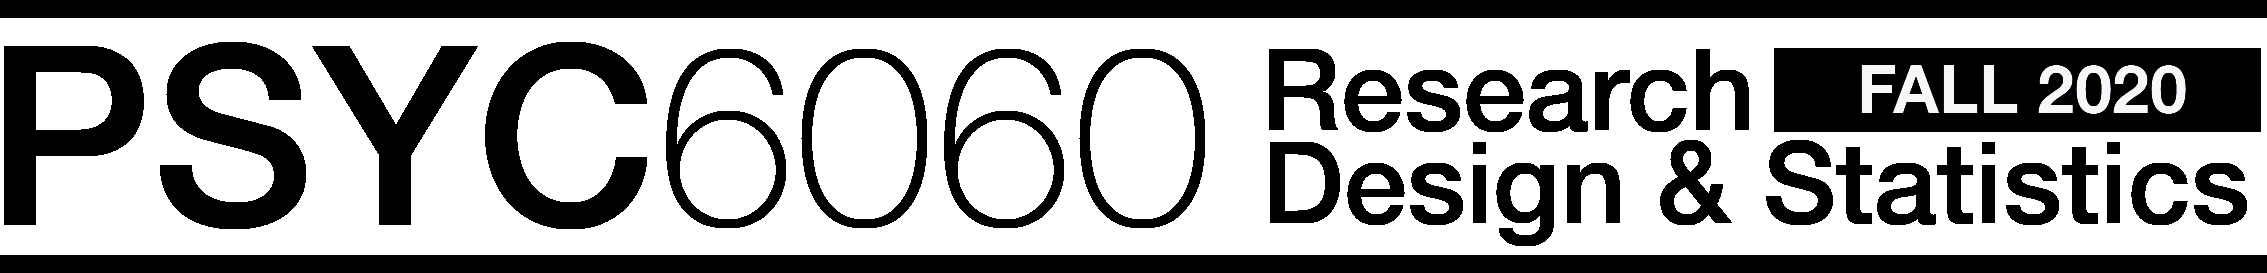
\includegraphics[width=1\linewidth]{header_6060}

These notes are a resource for students in my PSYC*6060 class. The notes are a subset of material that I am creating for a public domain statistics book to be released sometime in the distant future.

\hypertarget{about-the-author}{%
\chapter*{About the Author}\label{about-the-author}}


David J. Stanley is an Associate Professor of Industrial and Organizational Psychology at the University of Guelph in Canada. He obtained his PhD from Western University in London, Ontario. David has published articles in Advances in Methods and Practices in Psychological Science, Organizational Research Methods, Journal of Applied Psychology, Perspectives in Psychological Science, Journal of Business and Psychology, Journal of Vocational Behaviour, Journal of Personality and Social Psychology, Behavior Research Methods, Industrial and Organizational Psychology, and Emotion among other journals. David also created the apaTables R package.

\mainmatter

\hypertarget{introduction}{%
\chapter{Introduction}\label{introduction}}

Welcome! In this guide, we will teach you about statistics using the statistical software R with the interface provided by R Studio. The purpose of this chapter to is provide you with a set of activities that get you up-and-running in R quickly so get a sense of how it works. In later chatpers we will revisit these same topics in more detail.

\hypertarget{a-focus-on-workflow}{%
\section{A focus on workflow}\label{a-focus-on-workflow}}

An important part of this guide is training you in a workflow that will avoid many problems than can occur when using R.

\hypertarget{r-works-with-plug-ins}{%
\section{R works with plug-ins}\label{r-works-with-plug-ins}}

R is a statistical language with many plug-ins called \textbf{packages} that you will use for analyses. You can think of R as being like your smartphone. To do things with your phone you need \textbf{an App} (R equivalent: a \emph{package}) from the App Store (R equivalent: \emph{CRAN}). Apps need to be \textbf{downloaded} (R equivalent: \emph{install.packages}) before you can use them. To use the app you need \textbf{Open} it (R equivalent: \emph{library command}). These similarities are illustrated in Table \ref{tab:appstore} below.

\begin{table}

\caption{\label{tab:appstore}R packages are similar to smart phone apps (Kim, 2018)}
\centering
\begin{tabular}[t]{ll}
\toprule
Smart Phone Terminology & R Terminology\\
\midrule
App & package\\
App Store & CRAN\\
Download App from App Store & install.packages("apaTables", dependencies = TRUE)\\
Open App & library("apaTables")\\
\bottomrule
\end{tabular}
\end{table}

\hypertarget{create-an-account-at-r-studio-cloud}{%
\section{Create an account at R Studio Cloud}\label{create-an-account-at-r-studio-cloud}}

\href{http://www.rstudio.cloud}{R Studio Cloud} accounts are free and required for this guide. Please go to the website and set up a new account.

\hypertarget{join-the-class-workspace}{%
\section{Join the class workspace}\label{join-the-class-workspace}}

To do the assignment required for this class you need to join the class workspace on R Studio Cloud\index{R Studio Cloud}. To do so:

\begin{enumerate}
\def\labelenumi{\arabic{enumi}.}
\item
  Log into R Studio Cloud (if you haven't already done so).
\item
  Go to your university email account and find the message with the subject ``R Studio Workspace Invitation''. In this message there is a link to the class R Studio Cloud workspace.
\item
  Click on the workspace link in the email or paste it into your web browser. You should see a screen like the one below in Figure \ref{fig:join}. Click on the Join button.
\end{enumerate}

\begin{figure}
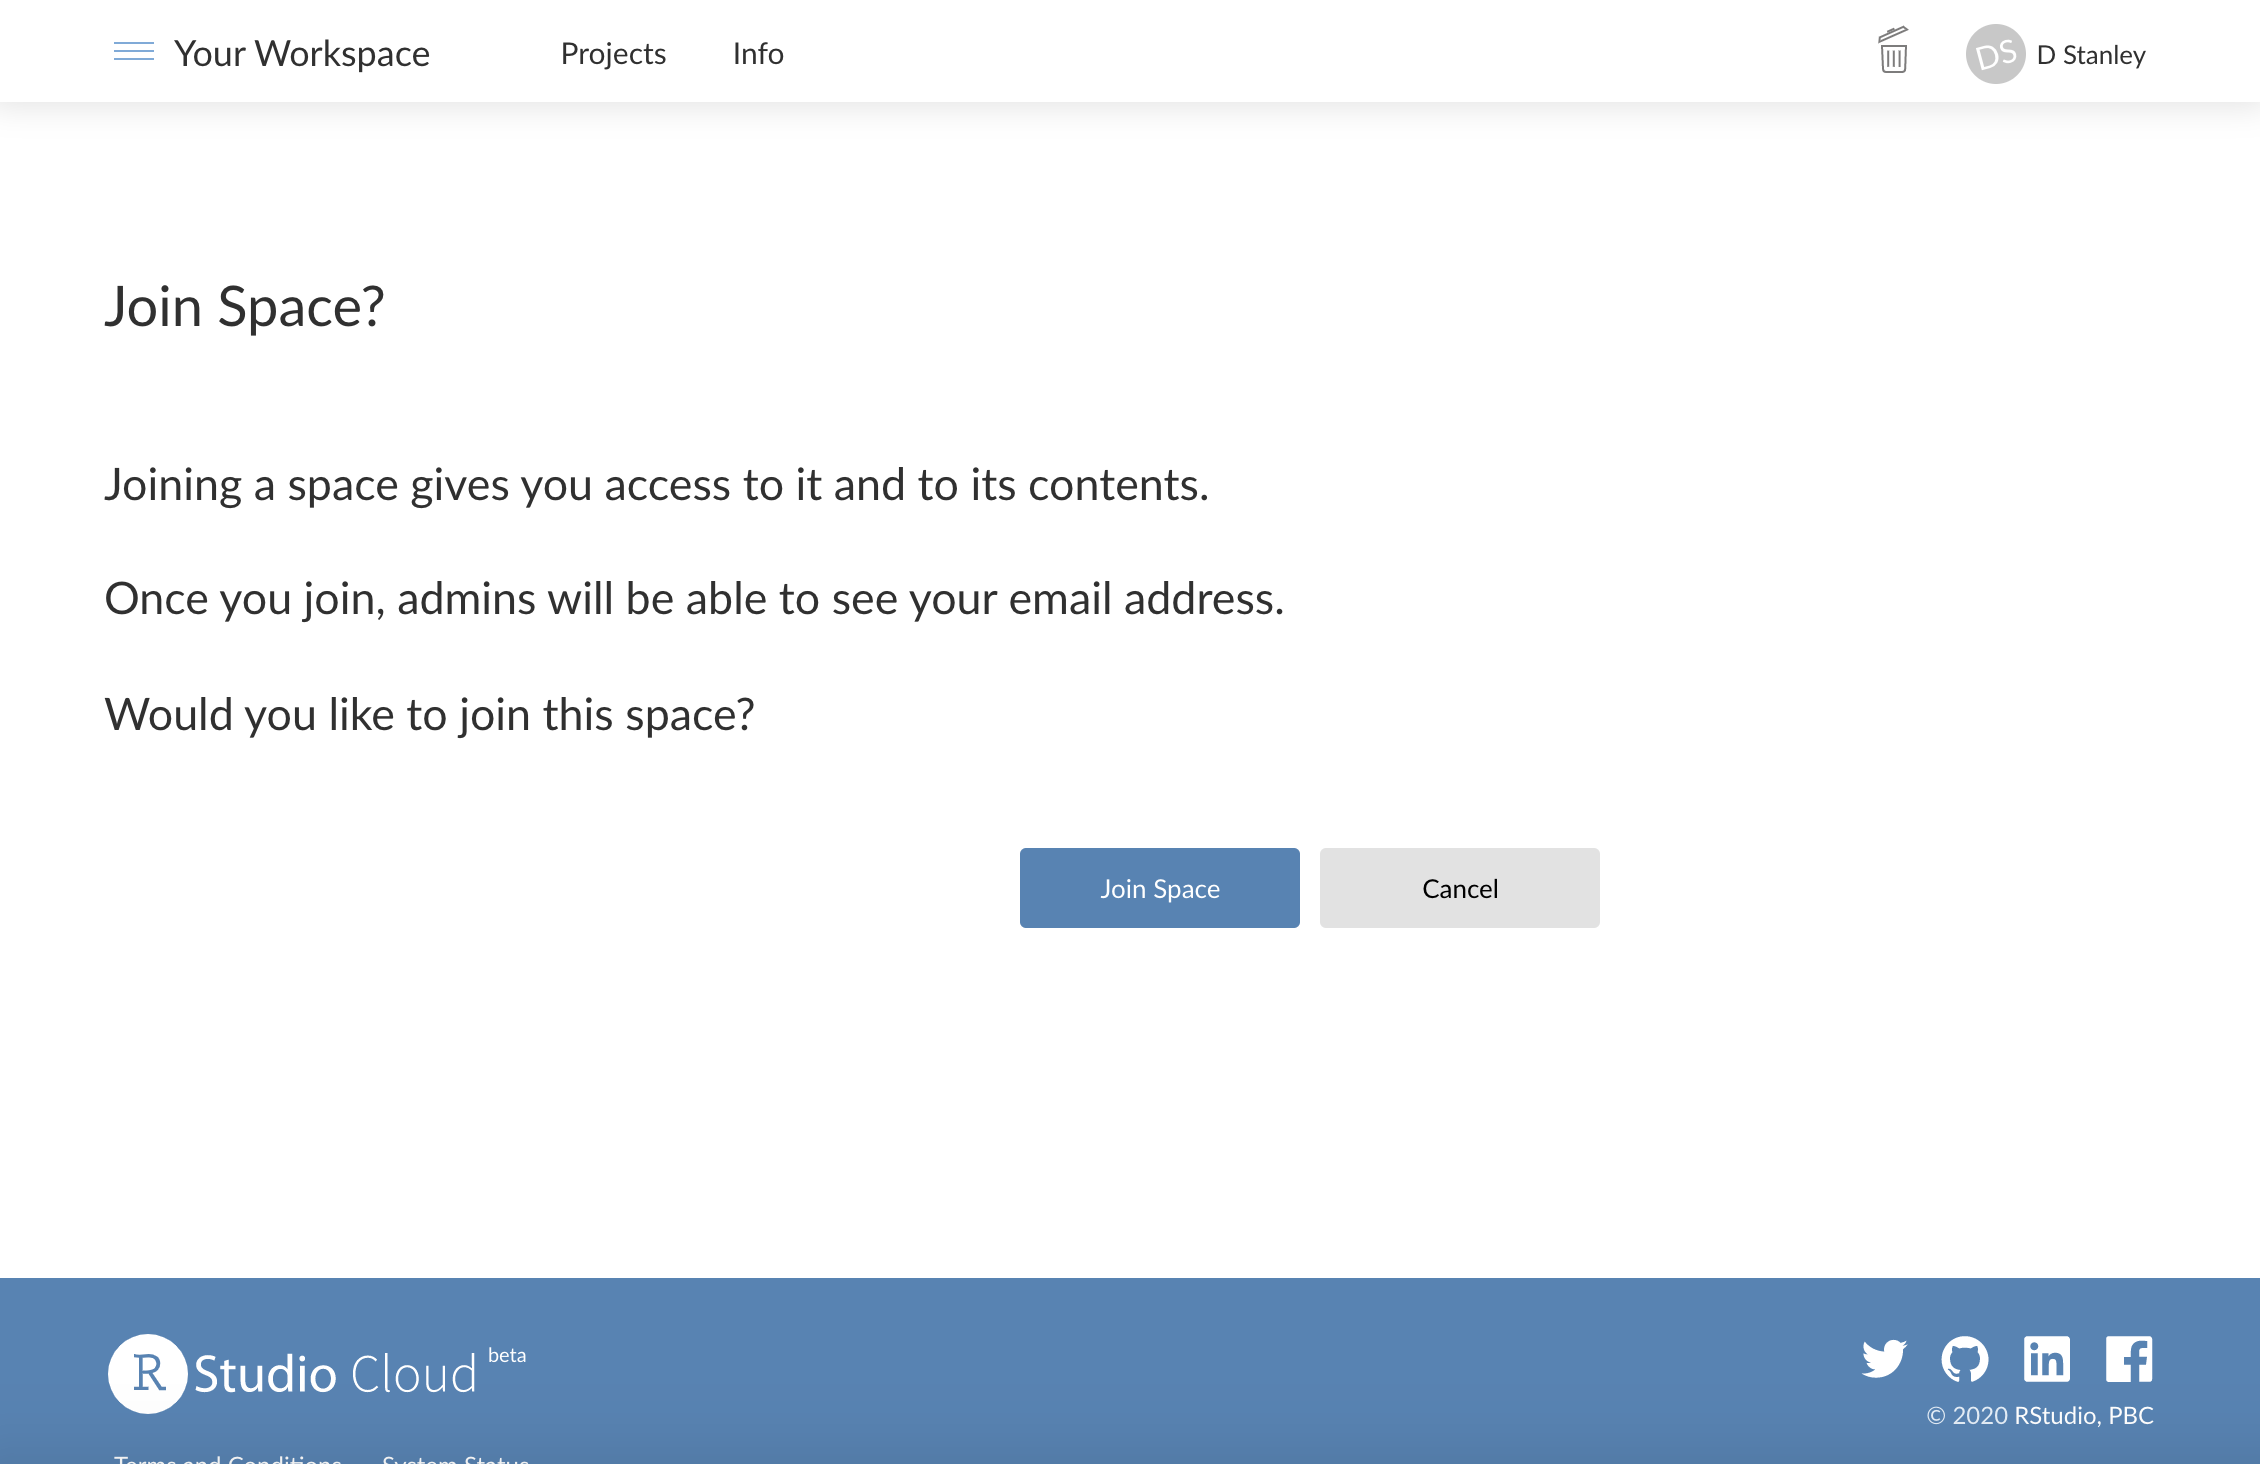
\includegraphics[width=0.7\linewidth]{ch_introduction/images/screenshot_join} \caption{Screenshot of workspace join message}\label{fig:join}
\end{figure}

\begin{enumerate}
\def\labelenumi{\arabic{enumi}.}
\setcounter{enumi}{3}
\tightlist
\item
  Then you should see the welcome message illustrated in Figure \ref{fig:welcome}. Above this message is the Projects menu option. Click on the word Project.
\end{enumerate}

\begin{figure}
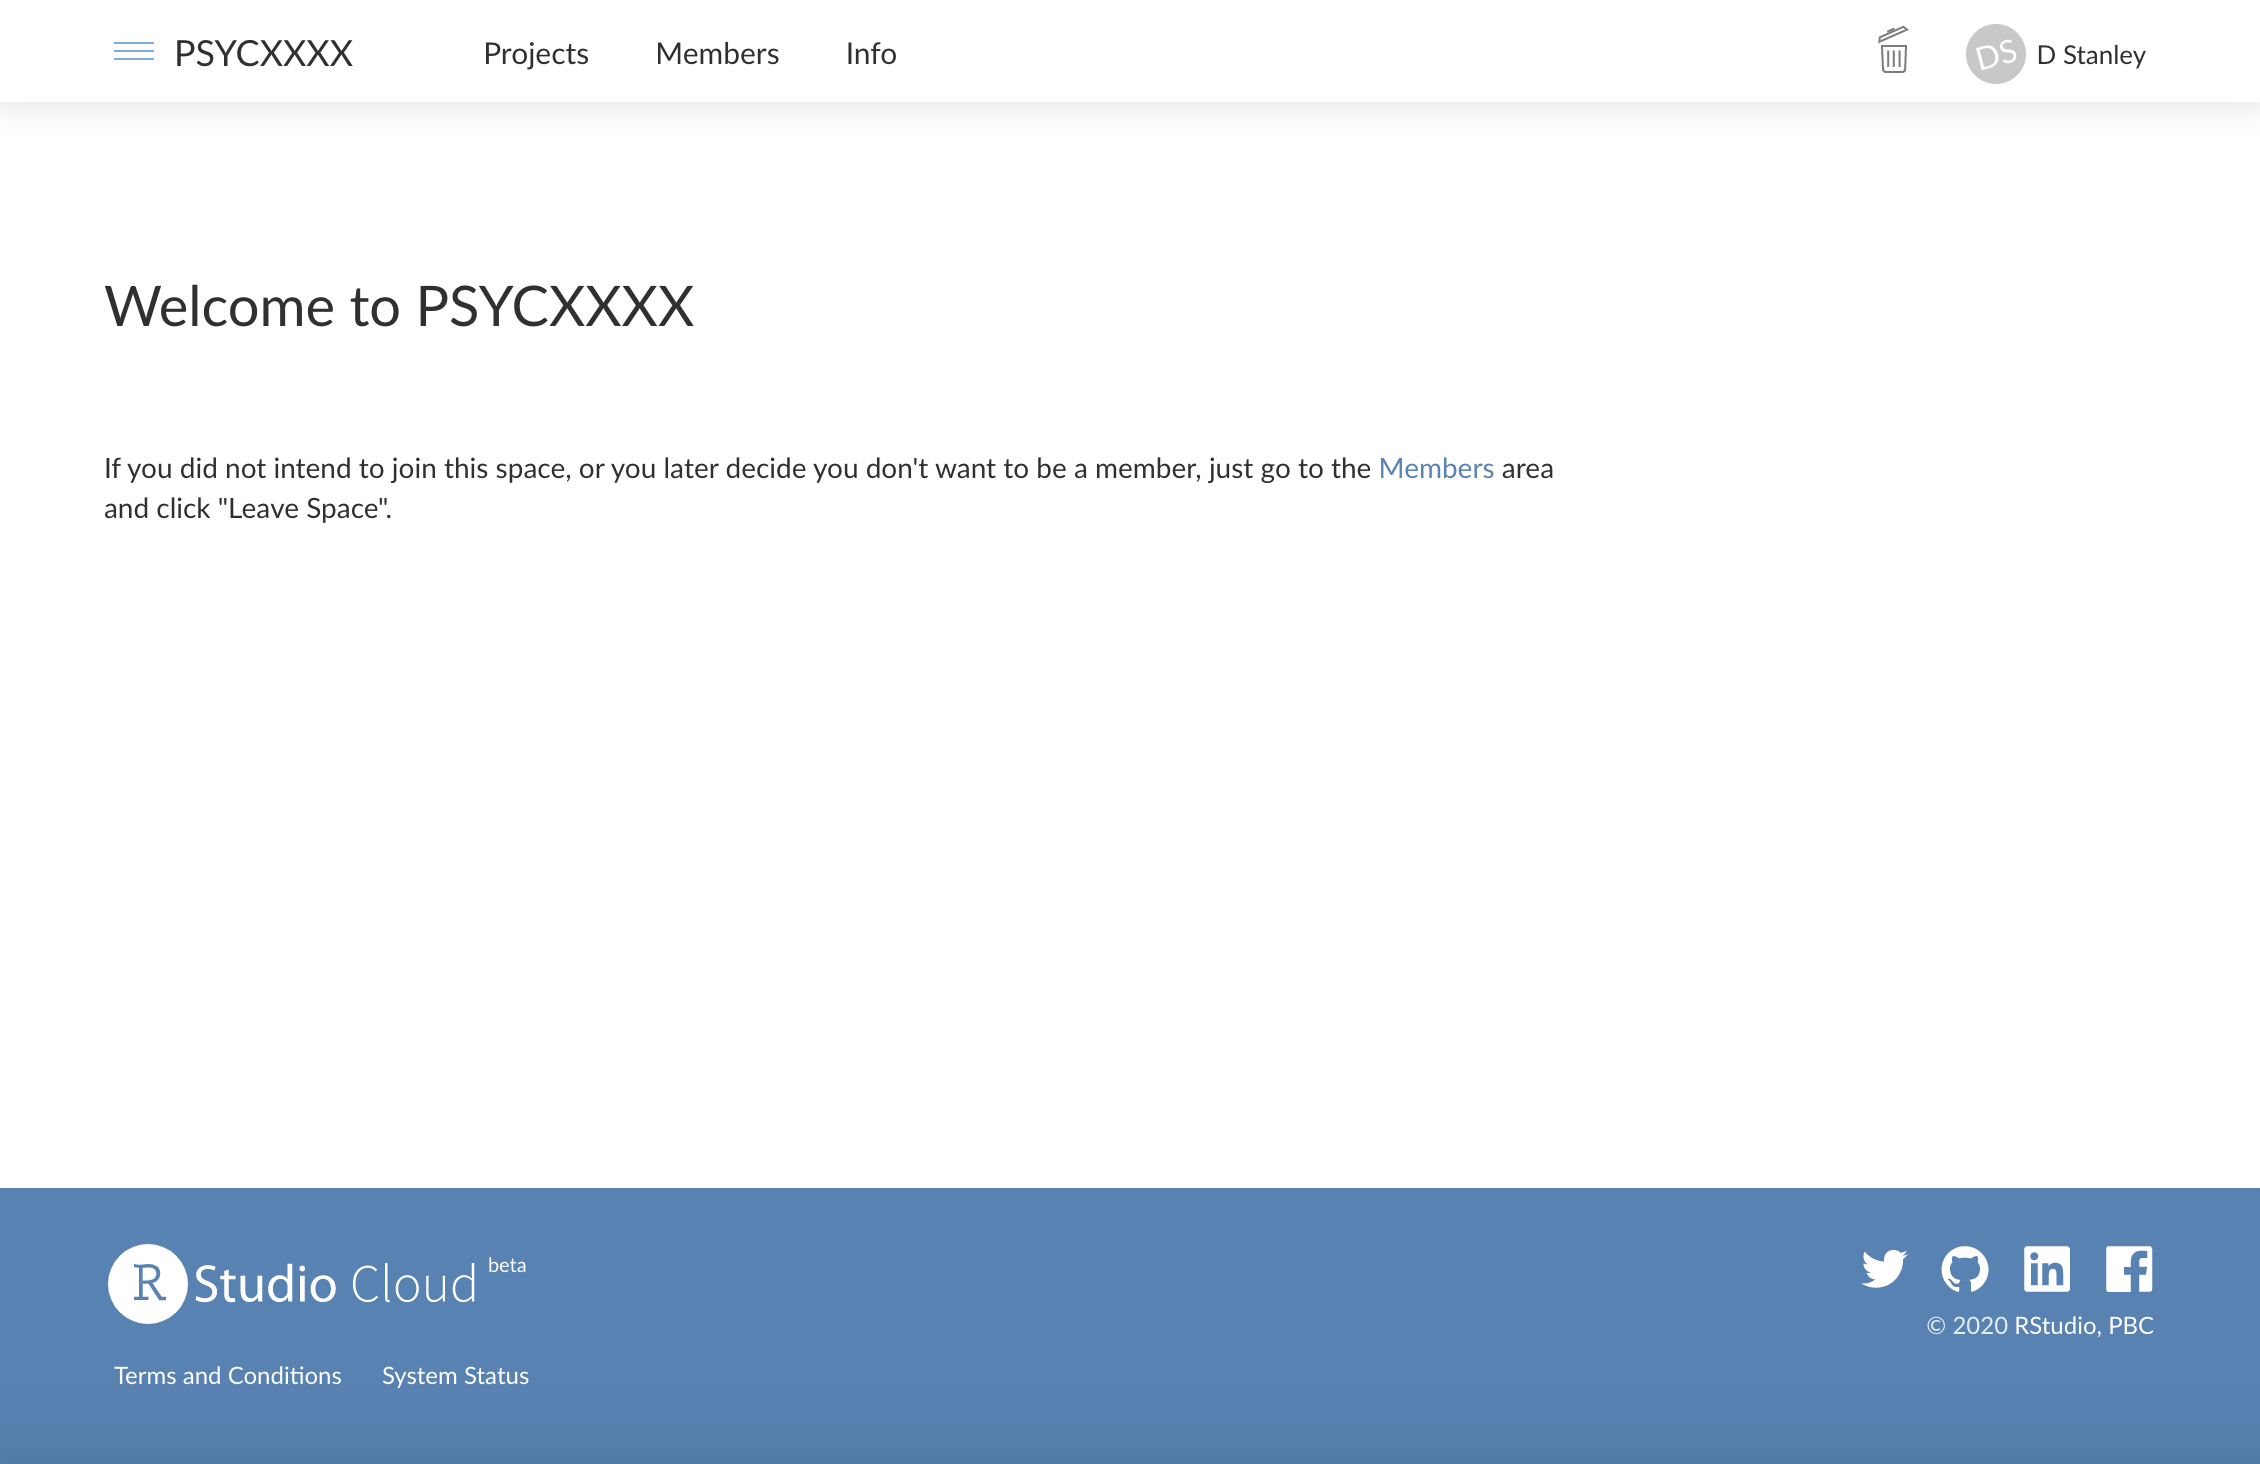
\includegraphics[width=0.7\linewidth]{ch_introduction/images/screenshot_welcome} \caption{Screenshot of welcome message}\label{fig:welcome}
\end{figure}

\begin{enumerate}
\def\labelenumi{\arabic{enumi}.}
\setcounter{enumi}{4}
\tightlist
\item
  You should now see the First Project displayed as in \ref{fig:assignment}. Click the Start button. You will then move to a view of R Studio.
\end{enumerate}

\begin{figure}
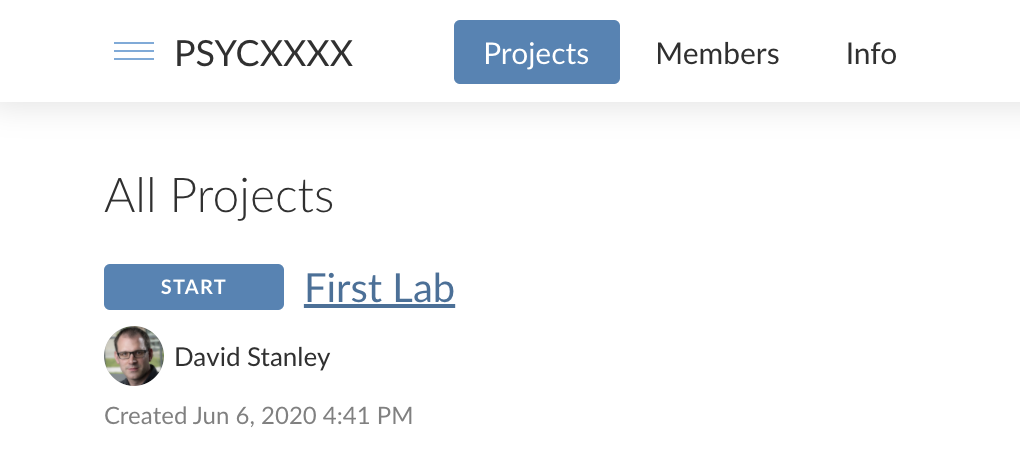
\includegraphics[width=0.7\linewidth]{ch_introduction/images/screenshot_assignment} \caption{Screenshot of starting first assignment}\label{fig:assignment}
\end{figure}

\begin{enumerate}
\def\labelenumi{\arabic{enumi}.}
\setcounter{enumi}{4}
\tightlist
\item
  In R Studio it is essential you use projects to keep your files organized and in the same spot. For this course, when your start an assignment on R Studio Cloud and the project will already have been made for you. Later you will learn to make your own R Studio Projects.
\end{enumerate}

\hypertarget{exploring-the-r-studio-interface}{%
\section{Exploring the R Studio Interface}\label{exploring-the-r-studio-interface}}

Once you have opened (or created) a Project folder, you are presented with the R Studio interface. There are a few key elements to the user interface that are illustrated in Figure \ref{fig:interface} In the lower right of the screen you can see the a panel with several tabs (i.e., Files, Plots, Packages, etc) that I will refer to as the Files pane. You look in this pane to see all the files associated with your project. On the left side of the screen is the Console which is an interactive pane where you type and obtain results in real time. I've placed two large grey blocks on the screen with text to more clearly identify the Console and Files panes. Not shown in this figure is the Script panel where we can store our commands for later reuse.

\begin{figure}
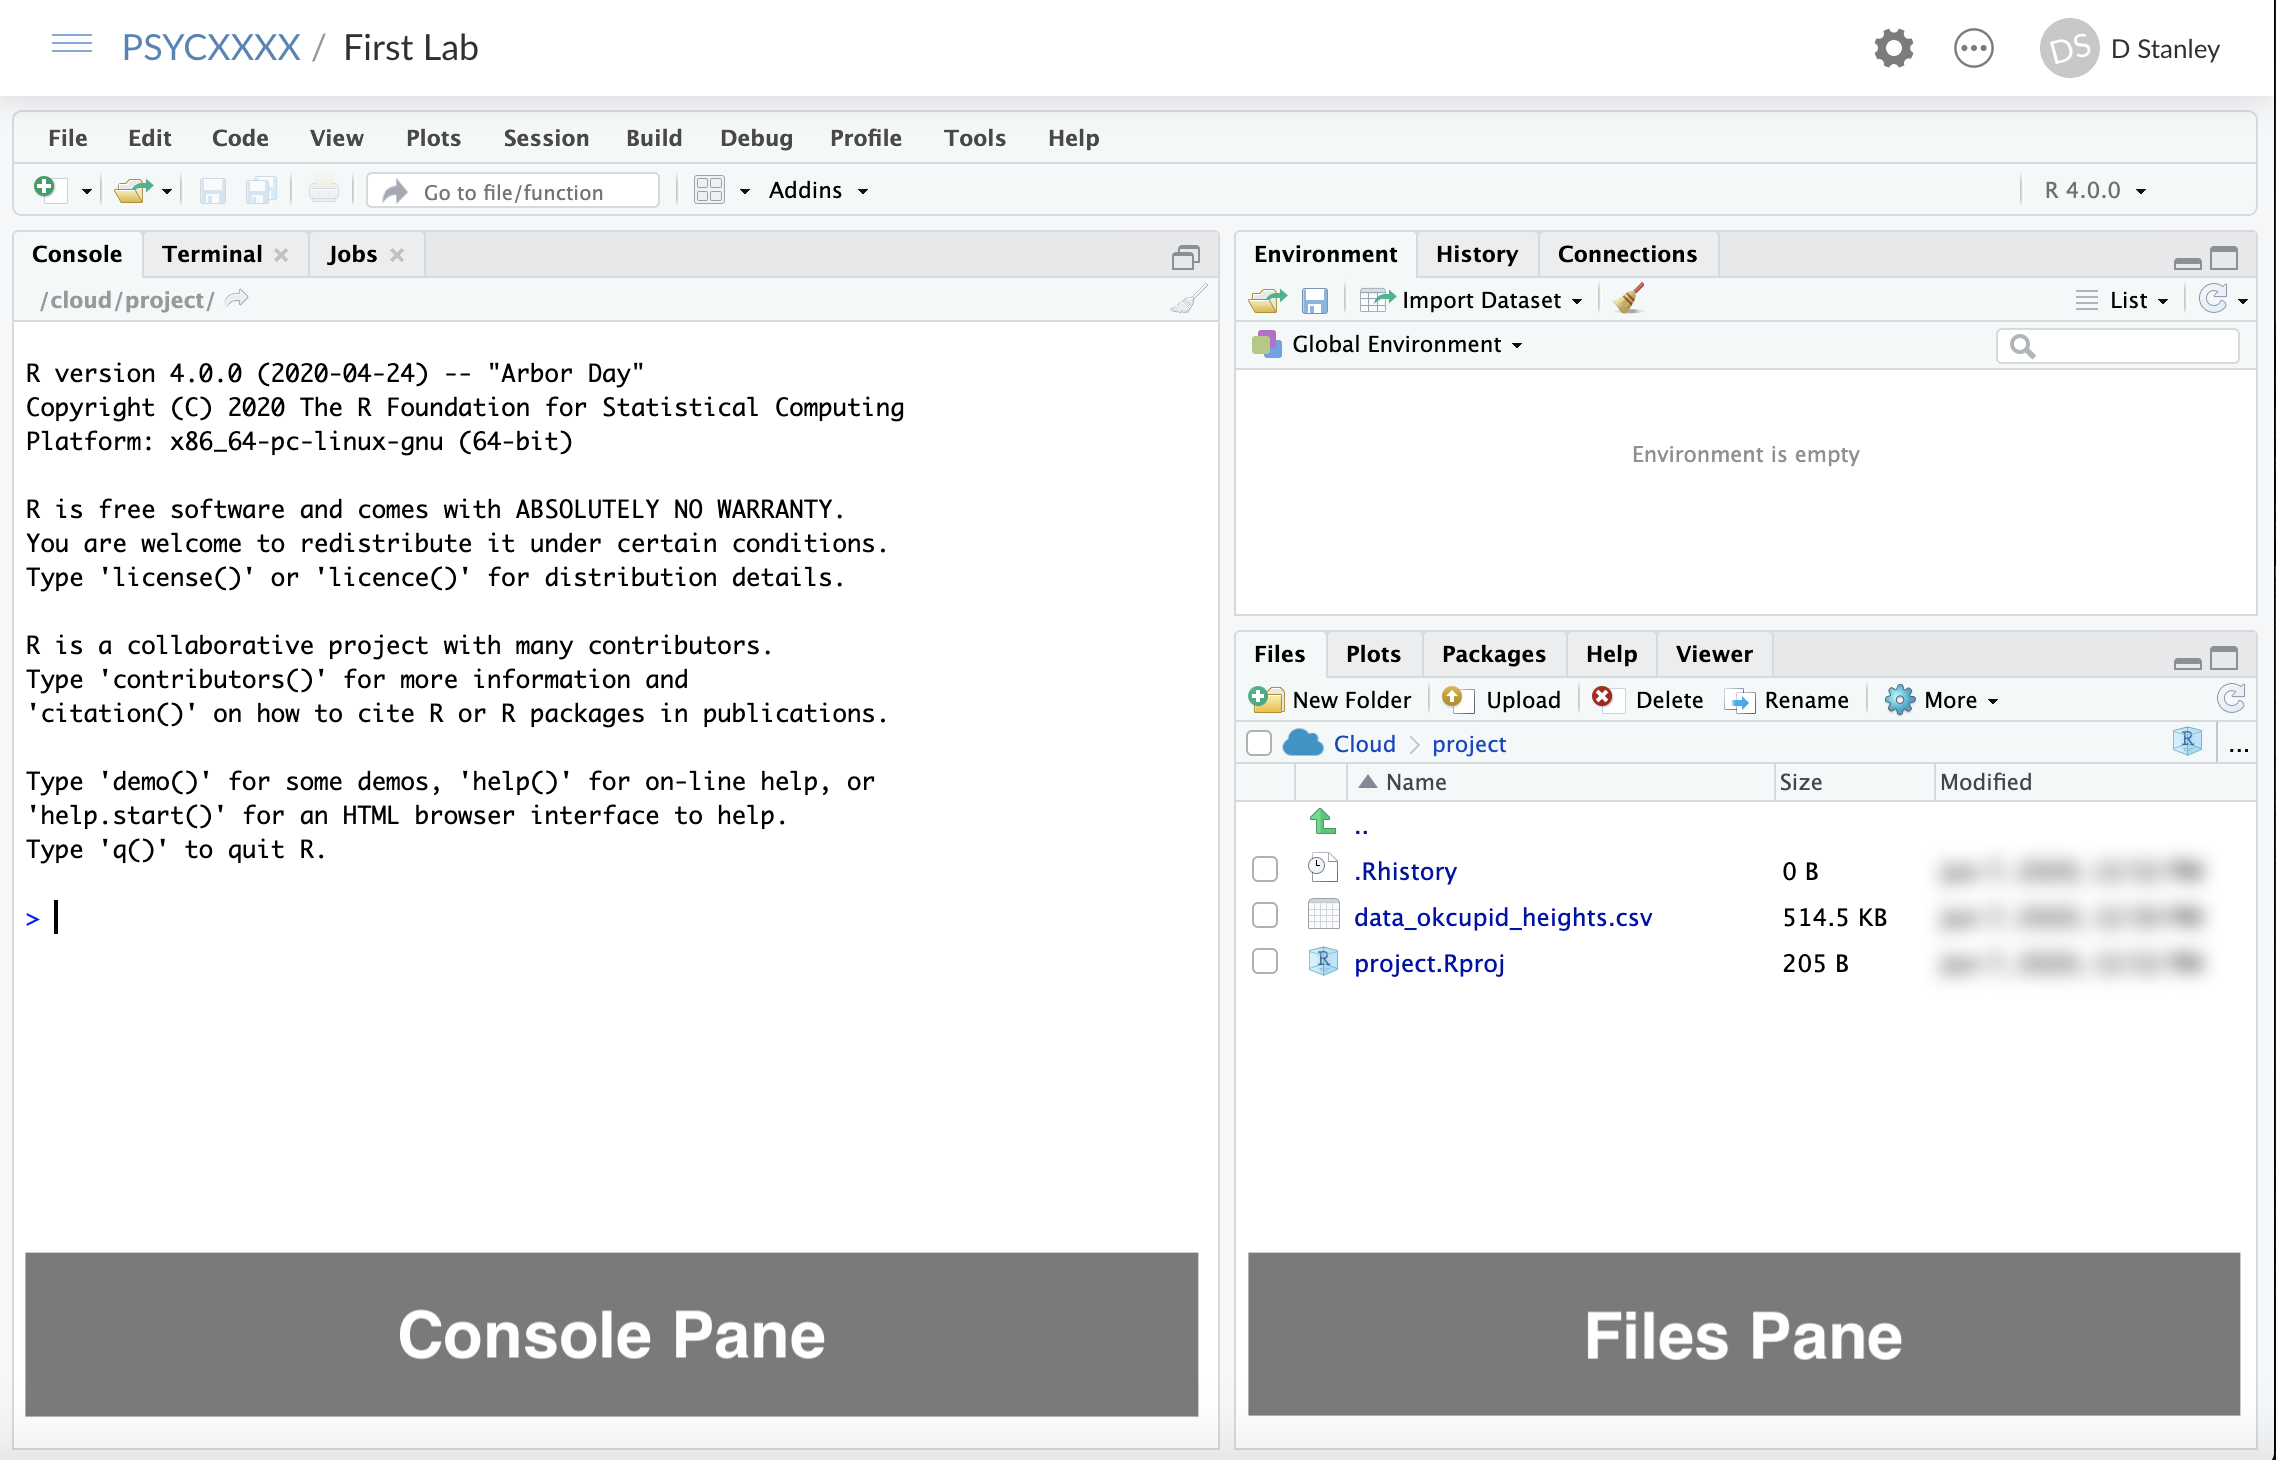
\includegraphics[width=0.7\linewidth]{ch_introduction/images/screenshot_interface} \caption{R Studio interface}\label{fig:interface}
\end{figure}

\hypertarget{console-panel}{%
\subsection{Console panel}\label{console-panel}}

When you first start R, the Console panel is on the left side of the screen. Sometimes there are two panels on the left side (one above the other); if so, the Console panel is the lower one (and labeled accordingly). We can use R a bit like a calculator. Try typing the following into the Console window: 8 + 6 + 7 + 5. You can see that R immediately produced the result on a line preceded by two hashtags (\#\#).

\begin{Shaded}
\begin{Highlighting}[]
\DecValTok{8} \OperatorTok{+}\StringTok{ }\DecValTok{6} \OperatorTok{+}\StringTok{ }\DecValTok{7} \OperatorTok{+}\StringTok{ }\DecValTok{5}
\end{Highlighting}
\end{Shaded}

\begin{verbatim}
## [1] 26
\end{verbatim}

We can also put the result into a variable to store it. Later we can use the print command to see that result. In the example below we add the numbers 3, 0, and 9 and store the result in the variable my\_sum. The text ``\textless-'' indicate you are putting what is on the right side of the arrow into the variable on the left side of the arrow. You can think of a variable as cup into which you can put different things. In this case, imagine a real-world cup with my\_sum written on the outside and inside the cup we have stored the sum of 3, 0, and 9 (i.e., 12).

\begin{Shaded}
\begin{Highlighting}[]
\NormalTok{my_sum <-}\StringTok{ }\DecValTok{3} \OperatorTok{+}\StringTok{ }\DecValTok{0} \OperatorTok{+}\StringTok{ }\DecValTok{9}
\end{Highlighting}
\end{Shaded}

We can inspect the contents of the my\_sum variable (i.e., my\_sum cup) with the print command:

\begin{Shaded}
\begin{Highlighting}[]
\KeywordTok{print}\NormalTok{(my_sum)}
\end{Highlighting}
\end{Shaded}

\begin{verbatim}
## [1] 12
\end{verbatim}

Variable are very useful in R. We will use them to store a single number, an entire data set,
the results of an analysis, or anything else.

\hypertarget{script-panel}{%
\subsection{Script Panel}\label{script-panel}}

Although you can use R with just with the Console panel, it's a better idea to use scripts via the Script panel - not visible yet. Scripts are just text files with the commands you use stored in them. You can run a script (as you will see below) using the Run or Source buttons located in the top right of the Script panel.

Scripts are valuable because if you need to run an analysis a second time you don't have to type the command in a second time. You can run the script again and again without retyping your commands. More importantly though, the script provides a record of your analyses.

A common problem in science is that after an article is published, the authors can't reproduce the numbers in the paper. You can read more about the important problem in a surprising article in the journal \href{https://molecularbrain.biomedcentral.com/articles/10.1186/s13041-020-0552-2}{Molecular Brain}. In this article an editor reports how a request for the data underlying articles resulted in the wrong data for 40 out of 41 papers. Long story short -- keep track of the data and scripts you use for your paper. In a later chapter, it's generally poor practice to manipulate or modify or analyze your data using any menu driven software because this approach does not provide a record of what you have done.

\hypertarget{writing-your-first-script}{%
\section{Writing your first script}\label{writing-your-first-script}}

\hypertarget{create-the-script-file}{%
\subsection{Create the script file}\label{create-the-script-file}}

Create a script in your R Studio project by using the menu File \textgreater{} New File \textgreater{} R Script.

Save the file with an appropriate name using the File menu. The file will be saved in your Project folder. A common, and good, convention for naming is to start all script names with the word ``script'' and separate words with an underscore. You might save this first script file with the name ``script\_my\_first\_one.R''. The advantage of beginning all script files with the word script is that when you look at your list of files alphabetically, all the script files will cluster together. Likewise, it's a good idea to save all data files such that they begin with ``data\_''. This way all the data files will cluster together in your directory view as well. You can see there is already a data file with this convention called ``data\_okcupid.csv''.

You can see as discussed previously, we are trying to instill an effective workflow as you learn R. Using a good naming convention (that is consistent with what others use) is part of the workflow. When you write your scripts it's a good idea to follow the \href{https://style.tidyverse.org}{tidyverse style guide} for script names, variable name, file names, and more.

\hypertarget{add-a-comment-to-your-script}{%
\subsection{Add a comment to your script}\label{add-a-comment-to-your-script}}

In the previous section you created your first script. We begin by adding a comment to the script. A comment is something that will be read by humans rather than the computer/R. You make comments for other people that will read your code and need to understand what you have done. However, realize that you are also making comments for your future self as illustrated in an \href{https://xkcd.com/1421/}{XKCD cartoon}.

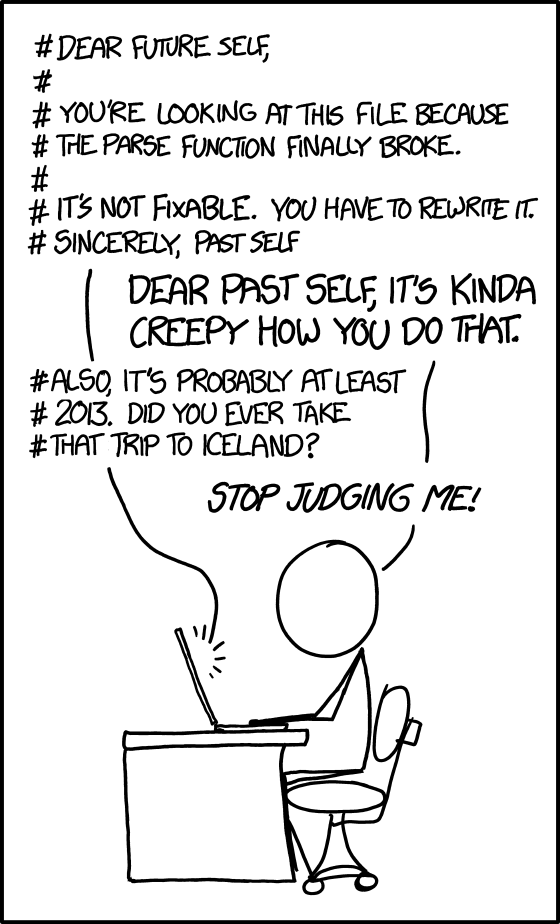
\includegraphics[width=0.4\linewidth]{ch_introduction/images/future_self_2x}

A good way to start every script is with a comment that includes the date of your script (or even better when you installed your packages, more on this later). Like smartphone apps, packages are updated regularly. Sometimes after a package is updated it will no longer work with an older script. Fortunately, the \href{https://cran.r-project.org/web/packages/checkpoint/index.html}{checkpoint package}\index{R Studio Cloud} lets users role back the clock and use older versions of packages. Adding a comment with the date of your script will help future users (including you) to use your script with the same version of the package used when you wrote the script. Dating your script is an important part of an effective and reproducible workflow.

\begin{Shaded}
\begin{Highlighting}[]
\CommentTok{# Code written on: YYYY/MM/DD }
\CommentTok{# By: John Smith}
\end{Highlighting}
\end{Shaded}

Moving forward, I suggest you use comments to make your own personal notes in your own code as your write it. Note that in the above comment I used the internationally accepted date format\index{date format} order Year/Month/Day created by the \href{https://www.iso.org/home.html}{International Organization for Standardization} (ISO). Some people use the mnemonic \emph{Your My Dream} to remember the \textbf{Y}ear \textbf{M}onth \textbf{D}ay order. Wikipedia provides more information about this \href{https://en.wikipedia.org/wiki/ISO_8601}{International Date Format (ISO 8601)}. An \href{https://xkcd.com/1179/}{XKCD} cartoon highlights the ISO date format:

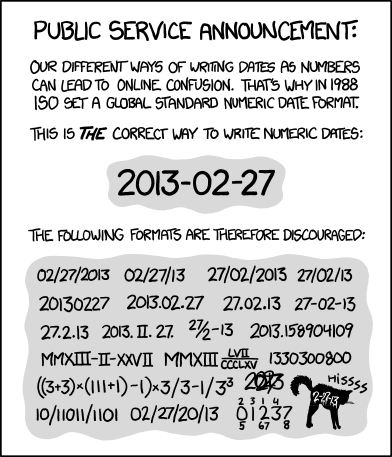
\includegraphics[width=0.4\linewidth]{ch_introduction/images/iso8601}

\hypertarget{background-about-the-tidyverse}{%
\subsection{Background about the tidyverse}\label{background-about-the-tidyverse}}

There are generally two broad ways of using R, the older way and the newer way. Using R the older way is refered to as using base R. A more modern approach to using R is the tidyverse\index{tidyverse}. The tidyverse represents a collection of packages the work together to give R a modern workflow. These packages do many things to help the data analyst (loading data, rearranging data, graphing, etc.). We will use the tidyverse approach to R in this guide.

A noted the tidyverse is a collection of packges. Each package adds new commands to R. The number of packges and correspondingly the number of new commands added to R by the tidyverse is large. Below is a list of the tidyverse packages:

\begin{verbatim}
##  [1] "broom"      "cli"        "crayon"     "dbplyr"    
##  [5] "dplyr"      "forcats"    "ggplot2"    "haven"     
##  [9] "hms"        "httr"       "jsonlite"   "lubridate" 
## [13] "magrittr"   "modelr"     "pillar"     "purrr"     
## [17] "readr"      "readxl"     "reprex"     "rlang"     
## [21] "rstudioapi" "rvest"      "stringr"    "tibble"    
## [25] "tidyr"      "xml2"       "tidyverse"
\end{verbatim}

Before you can use a package it needs to be installed -- this is the same as downloading an app from the App Store. Normally, you can install a \textbf{single} packages with the install.packages command. Previously, you needed run an install.package command for every package in the tidyverse as illustrated below (though we no longer use this approach).

\begin{Shaded}
\begin{Highlighting}[]
\CommentTok{# The old way of installing the tidyverse packages}
\CommentTok{# Like downloading apps from the app store}

\KeywordTok{install.packages}\NormalTok{(}\StringTok{"broom"}\NormalTok{, }\DataTypeTok{dep =} \OtherTok{TRUE}\NormalTok{)}
\KeywordTok{install.packages}\NormalTok{(}\StringTok{"cli"}\NormalTok{, }\DataTypeTok{dep =} \OtherTok{TRUE}\NormalTok{)}
\KeywordTok{install.packages}\NormalTok{(}\StringTok{"ggplot"}\NormalTok{, }\DataTypeTok{dep =} \OtherTok{TRUE}\NormalTok{)}
\CommentTok{# etc}
\end{Highlighting}
\end{Shaded}

Fortunately, the tidyverse packages can now by installed with a single install.packages command. Specifically, the install.packages command below will install all of the packages listed above.

\textbf{Class note: For the ``First Lab'', I've done the install.packages for you. So there is no need to use the install.packages command below in this first lab.}

\begin{Shaded}
\begin{Highlighting}[]
\KeywordTok{install.packages}\NormalTok{(}\StringTok{"tidyverse"}\NormalTok{, }\DataTypeTok{dep =} \OtherTok{TRUE}\NormalTok{)}
\end{Highlighting}
\end{Shaded}

\hypertarget{add-librarytidyverse-to-your-script}{%
\subsection{Add library(tidyverse) to your script}\label{add-librarytidyverse-to-your-script}}

The tidyverse is now installed, so we need to activate it. We do that with the library command. Put the library line below at the top of your script file (below your comment):

\begin{Shaded}
\begin{Highlighting}[]
\CommentTok{# Code written on: YYYY/MM/DD }
\CommentTok{# By: John Smith}
\KeywordTok{library}\NormalTok{(tidyverse)}
\end{Highlighting}
\end{Shaded}

\hypertarget{activate-tidyverse-auto-complete-for-your-script}{%
\subsection{Activate tidyverse auto-complete for your script}\label{activate-tidyverse-auto-complete-for-your-script}}

Select the library(tidyverse) text with your mouse/track-pad so that it is highlighted. Then click the Run button in the upper right of the Script panel. Doing this ``runs'' the selected text. After you click the Run button you should see text like the following the Console panel:

When you use library(tidyverse) to activate the tidyverse you activate the most commonly used subset of the tidyverse packages. In the output you see checkmarks beside names of the tidyverse packages you have activated.

By activating these packages you have added new commands to R that you will use. Sometimes these packages replace older versions of commands in R. The ``Conflicts'' section in the output shows you where the packages you activated replaced older R commands with newer R commands. You can activate the other tidyverse package by running a library command for each package -- if needed. No need to do so now.

Most importantly, running the library(tidyverse) prior to entering the rest of your script allows R Studio to present auto-complete options when typing your text. Remember to start each script with the library(tidyverse) command and then Run it so you get the autocomplete options for the rest of the commands your enter.

\hypertarget{loading-your-data}{%
\section{Loading your data}\label{loading-your-data}}

\hypertarget{use-read_csv-not-read.csv-to-open-files.}{%
\subsection{Use read\_csv (not read.csv) to open files.}\label{use-read_csv-not-read.csv-to-open-files.}}

If you inspect the Files pane on the right of the screen you see the \textbf{data\_okcupid.csv} data file in our project directory. We will load this data with the commands below. If you followed the steps above, you should have auto-complete for the tidyverse commands you type for now in -- in the current R session. Enter the command below into your script. As your start to type read\_csv you will likely be presented with an auto-complete option. You can use the arrow keys to move up and down the list of options to select the one you want - then press tab to select it.

Once your command looks like the one below select the text and click on the ``Run'' button.

Note: If you are not in the class, the data file is available from: \url{https://github.com/dstanley4/psyc6060bookdown}

\begin{Shaded}
\begin{Highlighting}[]
\NormalTok{okcupid_profiles <-}\StringTok{ }\KeywordTok{read_csv}\NormalTok{(}\DataTypeTok{file =} \StringTok{"data_okcupid.csv"}\NormalTok{)}
\end{Highlighting}
\end{Shaded}

\begin{verbatim}
## Parsed with column specification:
## cols(
##   age = col_double(),
##   diet = col_character(),
##   height = col_double(),
##   pets = col_character(),
##   sex = col_character(),
##   status = col_character()
## )
\end{verbatim}

The output indicates that you have loaded a data file and the type of data in each column. The sex column is of type col\_character which indicates it contains text/letters. Most of the columns are of the type character. The age and height columns contain numbers are correspondingly indicated to be the type col\_double. The label col\_double indicates that a column of numbers represented in R with \href{https://en.wikipedia.org/wiki/Double-precision_floating-point_format}{high precision}. There are other ways of representing numbers in R but this is the type we will see/use most often.

\hypertarget{checking-out-your-data}{%
\section{Checking out your data}\label{checking-out-your-data}}

There many ways of viewing the actual data you loaded. A few of these are illustrated now.

\hypertarget{view-see-a-spreadsheet-view-of-your-data}{%
\subsection{view(): See a spreadsheet view of your data}\label{view-see-a-spreadsheet-view-of-your-data}}

You can inspect your data in a spreadsheet view by using the view command. Do NOT add this command to your script file -- EVER. Adding it to the script can cause substantial problems. Type this command in the Console.

\begin{Shaded}
\begin{Highlighting}[]
\KeywordTok{view}\NormalTok{(okcupid_profiles)}
\end{Highlighting}
\end{Shaded}

\hypertarget{print-see-you-data-in-the-console}{%
\subsection{print(): See you data in the Console}\label{print-see-you-data-in-the-console}}

You can inspect the first few rows of your data with the print() command. It is OK to add a print command to your script. Try the print() command below in the Console:

\begin{Shaded}
\begin{Highlighting}[]
\KeywordTok{print}\NormalTok{(okcupid_profiles)}
\end{Highlighting}
\end{Shaded}

\begin{verbatim}
## # A tibble: 59,946 x 6
##      age diet         height pets              sex   status 
##    <dbl> <chr>         <dbl> <chr>             <chr> <chr>  
##  1    22 strictly an~     75 likes dogs and l~ m     single 
##  2    35 mostly other     70 likes dogs and l~ m     single 
##  3    38 anything         68 has cats          m     availa~
##  4    23 vegetarian       71 likes cats        m     single 
##  5    29 <NA>             66 likes dogs and l~ m     single 
##  6    29 mostly anyt~     67 likes cats        m     single 
##  7    32 strictly an~     65 likes dogs and l~ f     single 
##  8    31 mostly anyt~     65 likes dogs and l~ f     single 
##  9    24 strictly an~     67 likes dogs and l~ f     single 
## 10    37 mostly anyt~     65 likes dogs and l~ m     single 
## # ... with 59,936 more rows
\end{verbatim}

\hypertarget{head-check-out-the-first-few-rows-of-data}{%
\subsection{head(): Check out the first few rows of data}\label{head-check-out-the-first-few-rows-of-data}}

You can inspect the first few rows of your data with the head() command. Try the command below in the Console:

\begin{Shaded}
\begin{Highlighting}[]
\KeywordTok{head}\NormalTok{(okcupid_profiles)}
\end{Highlighting}
\end{Shaded}

\begin{verbatim}
## # A tibble: 6 x 6
##     age diet          height pets              sex   status 
##   <dbl> <chr>          <dbl> <chr>             <chr> <chr>  
## 1    22 strictly any~     75 likes dogs and l~ m     single 
## 2    35 mostly other      70 likes dogs and l~ m     single 
## 3    38 anything          68 has cats          m     availa~
## 4    23 vegetarian        71 likes cats        m     single 
## 5    29 <NA>              66 likes dogs and l~ m     single 
## 6    29 mostly anyth~     67 likes cats        m     single
\end{verbatim}

You can be even more specific and indicate you only want the first three row of your data with the head() command. Try the command below in the Console:

\begin{Shaded}
\begin{Highlighting}[]
\KeywordTok{head}\NormalTok{(okcupid_profiles, }\DecValTok{3}\NormalTok{)}
\end{Highlighting}
\end{Shaded}

\begin{verbatim}
## # A tibble: 3 x 6
##     age diet          height pets              sex   status 
##   <dbl> <chr>          <dbl> <chr>             <chr> <chr>  
## 1    22 strictly any~     75 likes dogs and l~ m     single 
## 2    35 mostly other      70 likes dogs and l~ m     single 
## 3    38 anything          68 has cats          m     availa~
\end{verbatim}

\hypertarget{tail-check-out-the-last-few-rows-of-data}{%
\subsection{tail(): Check out the last few rows of data}\label{tail-check-out-the-last-few-rows-of-data}}

You can inspect the last few rows of your data with the tail() command. Try the command below in the Console:

\begin{Shaded}
\begin{Highlighting}[]
\KeywordTok{tail}\NormalTok{(okcupid_profiles)}
\end{Highlighting}
\end{Shaded}

\begin{verbatim}
## # A tibble: 6 x 6
##     age diet         height pets                sex   status
##   <dbl> <chr>         <dbl> <chr>               <chr> <chr> 
## 1    31 <NA>             62 likes dogs          f     single
## 2    59 <NA>             62 has dogs            f     single
## 3    24 mostly anyt~     72 likes dogs and lik~ m     single
## 4    42 mostly anyt~     71 <NA>                m     single
## 5    27 mostly anyt~     73 likes dogs and lik~ m     single
## 6    39 <NA>             68 likes dogs and lik~ m     single
\end{verbatim}

You can be even more specific and indicate you only want the last three row of your data with the tail() command. Try the command below in the Console:

\begin{Shaded}
\begin{Highlighting}[]
\KeywordTok{tail}\NormalTok{(okcupid_profiles, }\DecValTok{3}\NormalTok{)}
\end{Highlighting}
\end{Shaded}

\begin{verbatim}
## # A tibble: 3 x 6
##     age diet         height pets                sex   status
##   <dbl> <chr>         <dbl> <chr>               <chr> <chr> 
## 1    42 mostly anyt~     71 <NA>                m     single
## 2    27 mostly anyt~     73 likes dogs and lik~ m     single
## 3    39 <NA>             68 likes dogs and lik~ m     single
\end{verbatim}

\hypertarget{summary-quick-summaries}{%
\subsection{summary(): Quick summaries}\label{summary-quick-summaries}}

You can a short summary of your data with the summary() command. Note that we will use the summary() command in many places in the guide. The output of the summary() command changes depending on what you give it - that is put inside the brackets. You can give the summary() command many things such as data, the results of a regression analysis, etc.

Try the command below in the Console. You will see that summary() give the mean and median for each of the numeric variables (age and height).

\begin{Shaded}
\begin{Highlighting}[]
\KeywordTok{summary}\NormalTok{(okcupid_profiles)}
\end{Highlighting}
\end{Shaded}

\begin{verbatim}
##       age            diet               height    
##  Min.   : 18.0   Length:59946       Min.   : 1.0  
##  1st Qu.: 26.0   Class :character   1st Qu.:66.0  
##  Median : 30.0   Mode  :character   Median :68.0  
##  Mean   : 32.3                      Mean   :68.3  
##  3rd Qu.: 37.0                      3rd Qu.:71.0  
##  Max.   :110.0                      Max.   :95.0  
##                                     NA's   :3     
##      pets               sex               status         
##  Length:59946       Length:59946       Length:59946      
##  Class :character   Class :character   Class :character  
##  Mode  :character   Mode  :character   Mode  :character  
##                                                          
##                                                          
##                                                          
## 
\end{verbatim}

\hypertarget{run-vs.-source-with-echo-vs.-source}{%
\section{\texorpdfstring{Run \emph{vs.} Source with Echo \emph{vs.} Source}{Run vs. Source with Echo vs. Source}}\label{run-vs.-source-with-echo-vs.-source}}

There are different ways of running commands in R. So far you have used two of these. You can enter them into the Console as we have done already. Or you can put them in your script select the text and clickk the Run button. There are four ways of running commands in your script.

You can:

\begin{enumerate}
\def\labelenumi{\arabic{enumi}.}
\tightlist
\item
  Console: Enter commands directly
\item
  Script: Select the command(s) and press the Run button.
\item
  Script: Source (Without Echo)
\item
  Script: Source With Echo
\end{enumerate}

Two of these approaches involve using the Source button, see Figure \ref{fig:sourcebutton}. You bring up the options for the Source button, illustrated in this figure, by clicking on the small arrow to the right of the word Source.

\begin{figure}
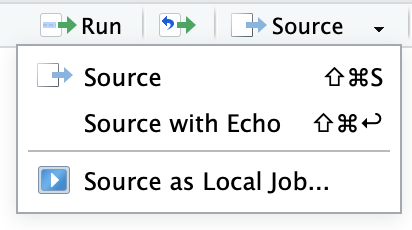
\includegraphics[width=0.35\linewidth]{ch_introduction/images/screenshot_source} \caption{Source button options}\label{fig:sourcebutton}
\end{figure}

\hypertarget{run-select-text}{%
\subsection{Run select text}\label{run-select-text}}

The Run button will run the text you highlight and present the relevant output. You have used this command a fair amount already.

I strongly suggest you ONLY use the Run button when testing a command to make sure it works or to debug a script. Or to run library(tidyverse) as you start working on your script so that you get the autocomplete options.

In general, you should always try to execute your R Scripts using the Source with Echo command (preceded by a Restart, see below). This ensures your script will work beginning to end for you in the future and for others that attempt to use it. Using the Run button in an ad lib basis can create output that is not reproducible.

\hypertarget{source-without-echo}{%
\subsection{Source (without Echo)}\label{source-without-echo}}

Source (without Echo) is not designed for the typical analysis workflow. It is mostly helpful when you run simulations. When you run Source (without Echo) much of the output you would wish to read is suppressed. In general, avoid this option. If you use it, you often won't see what you want to see in the output.

\hypertarget{source-with-echo}{%
\subsection{Source with Echo}\label{source-with-echo}}

The Source with Echo command runs all of the contents of a script and presents the output in the R console. This is the approach you should use to running your scripts in most cases.

Prior to running Source with Echo (or just Source), it's always a good idea to restart R. This makes sure you clear the computer memory of any errors from any previous runs.

So you should do the following EVERY time you run your script.

\begin{enumerate}
\def\labelenumi{\arabic{enumi}.}
\tightlist
\item
  Use the menu item: \textbf{Session \textgreater{} Restart R}
\item
  Click the down arrow beside the Source button, and click on Source With Echo
\end{enumerate}

This will clear potentially problematic previous stats, run the script commands, and display the output in the Console. Moving forward we will use this approach for running scripts. Once you have used Source wiht Echo once, you can just click the Source button and it will use Source with Echo automatically (without the need to use the pull down option for selecting Source with Echo).

\begin{rmdcaution}
Using Restart R before you run a script, or R code in general, is a critical workflow tip.
\end{rmdcaution}

\hypertarget{trying-source-with-echo}{%
\section{Trying Source with Echo}\label{trying-source-with-echo}}

Put the head(), tail(), and summary() command we used previously into your script. Then save your script using using the File \textgreater{} Save menu. You script should appear as below.

\begin{Shaded}
\begin{Highlighting}[]
\CommentTok{# Code written on: YYYY/MM/DD }
\CommentTok{# By: John Smith}
\KeywordTok{library}\NormalTok{(tidyverse)}

\NormalTok{okcupid_profiles <-}\StringTok{ }\KeywordTok{read_csv}\NormalTok{(}\DataTypeTok{file =} \StringTok{"data_okcupid.csv"}\NormalTok{)}

\KeywordTok{head}\NormalTok{(okcupid_profiles)}

\KeywordTok{tail}\NormalTok{(okcupid_profiles)}

\KeywordTok{summary}\NormalTok{(okcupid_profiles)}
\end{Highlighting}
\end{Shaded}

Now do the following:

\begin{enumerate}
\def\labelenumi{\arabic{enumi}.}
\tightlist
\item
  Use the menu item: \textbf{Session \textgreater{} Restart R}
\item
  Click the down arrow beside the Source button, and click on Source With Echo
\end{enumerate}

You should see the output below:

\begin{Shaded}
\begin{Highlighting}[]
\CommentTok{# Code written on: YYYY/MM/DD }
\CommentTok{# By: John Smith}
\KeywordTok{library}\NormalTok{(tidyverse)}

\NormalTok{okcupid_profiles <-}\StringTok{ }\KeywordTok{read_csv}\NormalTok{(}\DataTypeTok{file =} \StringTok{"data_okcupid.csv"}\NormalTok{)}
\end{Highlighting}
\end{Shaded}

\begin{verbatim}
## Parsed with column specification:
## cols(
##   age = col_double(),
##   diet = col_character(),
##   height = col_double(),
##   pets = col_character(),
##   sex = col_character(),
##   status = col_character()
## )
\end{verbatim}

\begin{Shaded}
\begin{Highlighting}[]
\KeywordTok{head}\NormalTok{(okcupid_profiles)}
\end{Highlighting}
\end{Shaded}

\begin{verbatim}
## # A tibble: 6 x 6
##     age diet          height pets              sex   status 
##   <dbl> <chr>          <dbl> <chr>             <chr> <chr>  
## 1    22 strictly any~     75 likes dogs and l~ m     single 
## 2    35 mostly other      70 likes dogs and l~ m     single 
## 3    38 anything          68 has cats          m     availa~
## 4    23 vegetarian        71 likes cats        m     single 
## 5    29 <NA>              66 likes dogs and l~ m     single 
## 6    29 mostly anyth~     67 likes cats        m     single
\end{verbatim}

\begin{Shaded}
\begin{Highlighting}[]
\KeywordTok{tail}\NormalTok{(okcupid_profiles)}
\end{Highlighting}
\end{Shaded}

\begin{verbatim}
## # A tibble: 6 x 6
##     age diet         height pets                sex   status
##   <dbl> <chr>         <dbl> <chr>               <chr> <chr> 
## 1    31 <NA>             62 likes dogs          f     single
## 2    59 <NA>             62 has dogs            f     single
## 3    24 mostly anyt~     72 likes dogs and lik~ m     single
## 4    42 mostly anyt~     71 <NA>                m     single
## 5    27 mostly anyt~     73 likes dogs and lik~ m     single
## 6    39 <NA>             68 likes dogs and lik~ m     single
\end{verbatim}

\begin{Shaded}
\begin{Highlighting}[]
\KeywordTok{summary}\NormalTok{(okcupid_profiles)}
\end{Highlighting}
\end{Shaded}

\begin{verbatim}
##       age            diet               height    
##  Min.   : 18.0   Length:59946       Min.   : 1.0  
##  1st Qu.: 26.0   Class :character   1st Qu.:66.0  
##  Median : 30.0   Mode  :character   Median :68.0  
##  Mean   : 32.3                      Mean   :68.3  
##  3rd Qu.: 37.0                      3rd Qu.:71.0  
##  Max.   :110.0                      Max.   :95.0  
##                                     NA's   :3     
##      pets               sex               status         
##  Length:59946       Length:59946       Length:59946      
##  Class :character   Class :character   Class :character  
##  Mode  :character   Mode  :character   Mode  :character  
##                                                          
##                                                          
##                                                          
## 
\end{verbatim}

Congratulations you just ran your first script!

\hypertarget{a-few-key-points-about}{%
\section{A few key points about}\label{a-few-key-points-about}}

Sometimes you will need to send a command additional information. Moreover, that information often needs to be grouped together into a vector or a list before you can send it to the command. We'll learn more about doing so in the future but here is a quick over view of vectors and lists to provide a foundation for future chapters.

\hypertarget{vector-of-numbers}{%
\subsubsection{Vector of numbers}\label{vector-of-numbers}}

We can create a vector of only numbers using the ``c'' function - which you can think of as being short for ``combine'' (or concatenate). In the commands below we create a vector of a few even numbers called ``even\_numbers''.

\begin{Shaded}
\begin{Highlighting}[]
\NormalTok{even_numbers <-}\StringTok{ }\KeywordTok{c}\NormalTok{(}\DecValTok{2}\NormalTok{, }\DecValTok{4}\NormalTok{, }\DecValTok{6}\NormalTok{, }\DecValTok{8}\NormalTok{, }\DecValTok{10}\NormalTok{)}
\end{Highlighting}
\end{Shaded}

\begin{Shaded}
\begin{Highlighting}[]
\KeywordTok{print}\NormalTok{(even_numbers)}
\end{Highlighting}
\end{Shaded}

\begin{verbatim}
## [1]  2  4  6  8 10
\end{verbatim}

We can obtain the second number in the vector using the following notation:

\begin{Shaded}
\begin{Highlighting}[]
\KeywordTok{print}\NormalTok{(even_numbers[}\DecValTok{2}\NormalTok{])}
\end{Highlighting}
\end{Shaded}

\begin{verbatim}
## [1] 4
\end{verbatim}

\hypertarget{vector-of-characters}{%
\subsubsection{Vector of characters}\label{vector-of-characters}}

We can also create vectors using only characters. Note that I use \textbf{SHIFT RETURN} after each comma to move to the next line.

\begin{Shaded}
\begin{Highlighting}[]
\NormalTok{favourite_things <-}\StringTok{ }\KeywordTok{c}\NormalTok{(}\StringTok{"copper kettles"}\NormalTok{,}
                      \StringTok{"woolen mittens"}\NormalTok{,}
                      \StringTok{"brown paper packages"}\NormalTok{)}
\end{Highlighting}
\end{Shaded}

\begin{Shaded}
\begin{Highlighting}[]
\KeywordTok{print}\NormalTok{(favourite_things)}
\end{Highlighting}
\end{Shaded}

\begin{verbatim}
## [1] "copper kettles"       "woolen mittens"      
## [3] "brown paper packages"
\end{verbatim}

As before, can obtain the second item in the vector using the following notation:

\begin{Shaded}
\begin{Highlighting}[]
\KeywordTok{print}\NormalTok{(favourite_things[}\DecValTok{2}\NormalTok{])}
\end{Highlighting}
\end{Shaded}

\begin{verbatim}
## [1] "woolen mittens"
\end{verbatim}

\hypertarget{lists}{%
\subsection{Lists}\label{lists}}

Lists are similar to vectors in that you can create them and access items by their numeric position. Vectors must be all characters or all numbers. Lists can be a mix of characters or numbers. Most importantly items in lists can be accessed by their label. Note that I use \textbf{SHIFT RETURN} after each comma to move to the next line in the code below.

\begin{Shaded}
\begin{Highlighting}[]
\NormalTok{my_list <-}\StringTok{ }\KeywordTok{list}\NormalTok{(}\DataTypeTok{last_name =} \StringTok{"Smith"}\NormalTok{,}
                \DataTypeTok{first_name =} \StringTok{"John"}\NormalTok{,}
                \DataTypeTok{office_number =} \DecValTok{1913}\NormalTok{)}

\KeywordTok{print}\NormalTok{(my_list)}
\end{Highlighting}
\end{Shaded}

\begin{verbatim}
## $last_name
## [1] "Smith"
## 
## $first_name
## [1] "John"
## 
## $office_number
## [1] 1913
\end{verbatim}

You can access an item in a list using double brackets:

\begin{Shaded}
\begin{Highlighting}[]
\KeywordTok{print}\NormalTok{(my_list[}\DecValTok{2}\NormalTok{])}
\end{Highlighting}
\end{Shaded}

\begin{verbatim}
## $first_name
## [1] "John"
\end{verbatim}

You can access an item in a list by its label/name using the dollar sign:

\begin{Shaded}
\begin{Highlighting}[]
\KeywordTok{print}\NormalTok{(my_list}\OperatorTok{$}\NormalTok{last_name)}
\end{Highlighting}
\end{Shaded}

\begin{verbatim}
## [1] "Smith"
\end{verbatim}

\begin{Shaded}
\begin{Highlighting}[]
\KeywordTok{print}\NormalTok{(my_list}\OperatorTok{$}\NormalTok{office_number)}
\end{Highlighting}
\end{Shaded}

\begin{verbatim}
## [1] 1913
\end{verbatim}

\hypertarget{thats-it}{%
\section{That's it!}\label{thats-it}}

Congratulations! You've reached the end of the introduction to R. Take a break, have a cookie, and read some more about R tomorrow!

\hypertarget{handling-data-with-the-tidyverse}{%
\chapter{Handling Data with the Tidyverse}\label{handling-data-with-the-tidyverse}}

\hypertarget{required}{%
\section{Required}\label{required}}

The data files below are used in this chapter. The files are available at: \url{https://github.com/dstanley4/psyc6060bookdown}

\begin{longtable}[]{@{}l@{}}
\toprule
Required Data\tabularnewline
\midrule
\endhead
data\_okcupid.csv\tabularnewline
data\_experiment.csv\tabularnewline
\bottomrule
\end{longtable}

The following CRAN packages must be installed:

\begin{longtable}[]{@{}l@{}}
\toprule
Required CRAN Packages\tabularnewline
\midrule
\endhead
tidyverse\tabularnewline
\bottomrule
\end{longtable}

\hypertarget{objective}{%
\section{Objective}\label{objective}}

The objective of this chapter is to familiarize you with some key commands in the tidyverse. These commands are used in isolation of each other for the most part. In the next chapter we will use these commands in a more coordinated way as we load a data set and move it from raw data to data that is ready for analysis (i.e., analytic data). You can start this project by Starting the class assignment on R Studio Cloud that corresponds to the chapter name.

\hypertarget{using-the-console}{%
\section{Using the Console}\label{using-the-console}}

All of the commands in this chapter should be typed into the Console within R. If you see a command split over multiple lines, use SHIFT-RETURN (macOS) or SHIFT-ENTER (Windows) to move the next line that is part of the same command.

\hypertarget{basic-tidyverse-commands}{%
\section{Basic tidyverse commands}\label{basic-tidyverse-commands}}

If you inspect the Files tab on the lower-right panel in R Studio you will see the file data\_okcupid.csv. The code below loads that file.

\begin{Shaded}
\begin{Highlighting}[]
\KeywordTok{library}\NormalTok{(tidyverse)}
\NormalTok{okcupid_profiles <-}\StringTok{ }\KeywordTok{read_csv}\NormalTok{(}\StringTok{"data_okcupid.csv"}\NormalTok{)}
\end{Highlighting}
\end{Shaded}

You can see the first few rows of the data using the print() command. Each row presents a person whereas each column represents a variable. If you have a large number of columns you will only see the first several columns with this approach to viewing your data.

\begin{Shaded}
\begin{Highlighting}[]
\KeywordTok{print}\NormalTok{(okcupid_profiles)}
\end{Highlighting}
\end{Shaded}

\begin{verbatim}
## # A tibble: 59,946 x 6
##      age diet         height pets              sex   status 
##    <dbl> <chr>         <dbl> <chr>             <chr> <chr>  
##  1    22 strictly an~     75 likes dogs and l~ m     single 
##  2    35 mostly other     70 likes dogs and l~ m     single 
##  3    38 anything         68 has cats          m     availa~
##  4    23 vegetarian       71 likes cats        m     single 
##  5    29 <NA>             66 likes dogs and l~ m     single 
##  6    29 mostly anyt~     67 likes cats        m     single 
##  7    32 strictly an~     65 likes dogs and l~ f     single 
##  8    31 mostly anyt~     65 likes dogs and l~ f     single 
##  9    24 strictly an~     67 likes dogs and l~ f     single 
## 10    37 mostly anyt~     65 likes dogs and l~ m     single 
## # ... with 59,936 more rows
\end{verbatim}

But it's also helpful just to see a list of the columns in the data with the glimpse() command:

\begin{Shaded}
\begin{Highlighting}[]
\KeywordTok{glimpse}\NormalTok{(okcupid_profiles)}
\end{Highlighting}
\end{Shaded}

\begin{verbatim}
## Rows: 59,946
## Columns: 6
## $ age    <dbl> 22, 35, 38, 23, 29, 29, 32, 31, 24, 37, ...
## $ diet   <chr> "strictly anything", "mostly other", "an...
## $ height <dbl> 75, 70, 68, 71, 66, 67, 65, 65, 67, 65, ...
## $ pets   <chr> "likes dogs and likes cats", "likes dogs...
## $ sex    <chr> "m", "m", "m", "m", "m", "m", "f", "f", ...
## $ status <chr> "single", "single", "available", "single...
\end{verbatim}

The glimpse() command is useful because it quickly allows you to see all of the columns. Moreover, it allows you to see the type for each column. Types were briefly discussed in the last chapter. Notice in the output beside each column name that some columns are labeled ``dbl'' which is short for double -- a type of numeric column. Other columns are labeled ``chr'' which is short for character - meaning the columns contain characters. These designations will become important in the next chapter as we prepare data for analysis.

\hypertarget{select}{%
\subsection{select()}\label{select}}

The select() command allows you to obtain a subset of the columns in your data. The commands below can be used to obtain the age and height columns. You can read the command as: take the okcupid\_profiles data and then select the age and height columns. The ``\%\textgreater\%'' symbol can be read as ``and then''. You can see that this code prints out the data with just the age and height columns. Remember, use SHIFT-ENTER or SHIFT-RETURN to move to the next line in the block of code.

\begin{Shaded}
\begin{Highlighting}[]
\NormalTok{okcupid_profiles }\OperatorTok\StringTok{ }
\StringTok{  }\KeywordTok{select}\NormalTok{(age, height)}
\end{Highlighting}
\end{Shaded}

\begin{verbatim}
## # A tibble: 59,946 x 2
##      age height
##    <dbl>  <dbl>
##  1    22     75
##  2    35     70
##  3    38     68
##  4    23     71
##  5    29     66
##  6    29     67
##  7    32     65
##  8    31     65
##  9    24     67
## 10    37     65
## # ... with 59,936 more rows
\end{verbatim}

Of course, it's usually of little help to just print the subset of the data. It's better to store it in a new data. In the command below we store the resulting data in a new data set called new\_data.

\begin{Shaded}
\begin{Highlighting}[]
\NormalTok{new_data <-}\StringTok{ }\NormalTok{okcupid_profiles }\OperatorTok\StringTok{ }
\StringTok{  }\KeywordTok{select}\NormalTok{(age, height)}
\end{Highlighting}
\end{Shaded}

The glimpse() command shows us that only the age and height columns are in new\_data.

\begin{Shaded}
\begin{Highlighting}[]
\KeywordTok{glimpse}\NormalTok{(new_data)}
\end{Highlighting}
\end{Shaded}

\begin{verbatim}
## Rows: 59,946
## Columns: 2
## $ age    <dbl> 22, 35, 38, 23, 29, 29, 32, 31, 24, 37, ...
## $ height <dbl> 75, 70, 68, 71, 66, 67, 65, 65, 67, 65, ...
\end{verbatim}

In the above example we indicated the columns we wanted to retain from the okcupid\_profiles data using the select() command. However, we can also indicate the columns we want to drop from okcupid\_profiles using a minus sign (-) in front of the columns we specify in the select() command.

\begin{Shaded}
\begin{Highlighting}[]
\NormalTok{new_data <-}\StringTok{ }\NormalTok{okcupid_profiles }\OperatorTok\StringTok{ }\KeywordTok{select}\NormalTok{(}\OperatorTok{-}\NormalTok{age, }\OperatorTok{-}\NormalTok{height)}
\end{Highlighting}
\end{Shaded}

The glimpse() command shows us that we kept all the columns except the age and height columns when we created new\_data.

\begin{Shaded}
\begin{Highlighting}[]
\KeywordTok{glimpse}\NormalTok{(new_data)}
\end{Highlighting}
\end{Shaded}

\begin{verbatim}
## Rows: 59,946
## Columns: 4
## $ diet   <chr> "strictly anything", "mostly other", "an...
## $ pets   <chr> "likes dogs and likes cats", "likes dogs...
## $ sex    <chr> "m", "m", "m", "m", "m", "m", "f", "f", ...
## $ status <chr> "single", "single", "available", "single...
\end{verbatim}

\hypertarget{summarise}{%
\subsection{summarise()}\label{summarise}}

The summarise() command can be used to generate descriptive statistics for a specified column. You can easily calculate column descriptive statistics using the corresponding commands for mean(), sd(), min(), max(), among others. In the example below we calculate the mean for the age column.

In the code below, mean(age, na.rm = TRUE), indicates to R that it should calculate the mean of the age column. The na.rm indicates how missing values should be handled. The na stands for not available; in R missing values are classified as Not Available or NA. The rm stands for remove. Consequently, na.rm is asking: ``Should we remove missing values when calculating the mean?'' The TRUE indicates that yes, missing values should be removed when calculating the mean. The result of this calculation is placed into a variable labelled age\_mean, though we could have used any label we wanted instead of age\_mean. We see that the mean of the age column is, with rounding, 32.3.

\begin{Shaded}
\begin{Highlighting}[]
\NormalTok{okcupid_profiles }\OperatorTok\StringTok{ }
\StringTok{  }\KeywordTok{summarise}\NormalTok{(}\DataTypeTok{age_mean =} \KeywordTok{mean}\NormalTok{(age, }\DataTypeTok{na.rm =} \OtherTok{TRUE}\NormalTok{))}
\end{Highlighting}
\end{Shaded}

\begin{verbatim}
## # A tibble: 1 x 1
##   age_mean
##      <dbl>
## 1     32.3
\end{verbatim}

More than one calculation can occur in the same summarise() command. You can easily add the calculation for the standared deviation with the sd() command.

\begin{Shaded}
\begin{Highlighting}[]
\NormalTok{okcupid_profiles }\OperatorTok\StringTok{ }
\StringTok{  }\KeywordTok{summarise}\NormalTok{(}\DataTypeTok{age_mean =} \KeywordTok{mean}\NormalTok{(age, }\DataTypeTok{na.rm =} \OtherTok{TRUE}\NormalTok{),}
            \DataTypeTok{age_sd =} \KeywordTok{sd}\NormalTok{(age, }\DataTypeTok{na.rm =} \OtherTok{TRUE}\NormalTok{))}
\end{Highlighting}
\end{Shaded}

\begin{verbatim}
## # A tibble: 1 x 2
##   age_mean age_sd
##      <dbl>  <dbl>
## 1     32.3   9.45
\end{verbatim}

Often this process does too much rounding. We can get more exact results by adding an as.data.frame() to the end of the commands.

\begin{Shaded}
\begin{Highlighting}[]
\NormalTok{okcupid_profiles }\OperatorTok\StringTok{ }
\StringTok{  }\KeywordTok{summarise}\NormalTok{(}\DataTypeTok{age_mean =} \KeywordTok{mean}\NormalTok{(age, }\DataTypeTok{na.rm =} \OtherTok{TRUE}\NormalTok{),}
            \DataTypeTok{age_sd =} \KeywordTok{sd}\NormalTok{(age, }\DataTypeTok{na.rm =} \OtherTok{TRUE}\NormalTok{)) }\OperatorTok
\StringTok{  }\KeywordTok{as.data.frame}\NormalTok{()}
\end{Highlighting}
\end{Shaded}

\begin{verbatim}
##   age_mean age_sd
## 1    32.34  9.453
\end{verbatim}

\hypertarget{filter}{%
\subsection{filter()}\label{filter}}

The filter() command allows you to obtain a subset of the rows in your data. In the example below we create a new data set with just the males from the original data.

Notice the structure of the original data below in the glimpse() output. There is a column called sex that uses m and f to indicate male and female, respectively. Also notice that there are 59946 rows in the okcupid\_profiles data.

\begin{Shaded}
\begin{Highlighting}[]
\KeywordTok{glimpse}\NormalTok{(okcupid_profiles)}
\end{Highlighting}
\end{Shaded}

\begin{verbatim}
## Rows: 59,946
## Columns: 6
## $ age    <dbl> 22, 35, 38, 23, 29, 29, 32, 31, 24, 37, ...
## $ diet   <chr> "strictly anything", "mostly other", "an...
## $ height <dbl> 75, 70, 68, 71, 66, 67, 65, 65, 67, 65, ...
## $ pets   <chr> "likes dogs and likes cats", "likes dogs...
## $ sex    <chr> "m", "m", "m", "m", "m", "m", "f", "f", ...
## $ status <chr> "single", "single", "available", "single...
\end{verbatim}

We use the filter command to select a subset of the rows based on the content of any column. In this case the sex column is used to obtain a subset of the rows; the rows with the value ``m'' are obtained. Notice the double equals sign is used to indicate ``equal to''. The reason a double equals sign is used here (instead of a single equals sign) is to distinguish it from the use of the single equals sign in the summarise command above. In the summarise command above, the single equal sign was used to indicate ``assign to''. That is, assign to age\_mean the mean of the column age after it is calculated. A single equals sign indicates ``assign to'' whereas a double equals sign indicates ``is equal to''.

\begin{Shaded}
\begin{Highlighting}[]
\NormalTok{okcupid_males <-}\StringTok{ }\NormalTok{okcupid_profiles }\OperatorTok
\StringTok{  }\KeywordTok{filter}\NormalTok{(sex }\OperatorTok{==}\StringTok{ "m"}\NormalTok{)}
\end{Highlighting}
\end{Shaded}

We use glimpse() to inspect these all male data. Notice that only the letter m is in the sex column - indicating only males are in the data set. Also notice that there are 35829 rows in the okcupid\_males data - fewer people because males are a subset of the total number of rows.

\begin{Shaded}
\begin{Highlighting}[]
\KeywordTok{glimpse}\NormalTok{(okcupid_males)}
\end{Highlighting}
\end{Shaded}

\begin{verbatim}
## Rows: 35,829
## Columns: 6
## $ age    <dbl> 22, 35, 38, 23, 29, 29, 37, 35, 28, 24, ...
## $ diet   <chr> "strictly anything", "mostly other", "an...
## $ height <dbl> 75, 70, 68, 71, 66, 67, 65, 70, 72, 72, ...
## $ pets   <chr> "likes dogs and likes cats", "likes dogs...
## $ sex    <chr> "m", "m", "m", "m", "m", "m", "m", "m", ...
## $ status <chr> "single", "single", "available", "single...
\end{verbatim}

The filter command can be combined with the summarise command to get the descriptive statistics for males without the hassle of creating new data. This is again done using the \%\textgreater\% ``and then'' operator.

\begin{Shaded}
\begin{Highlighting}[]
\NormalTok{okcupid_profiles }\OperatorTok
\StringTok{  }\KeywordTok{filter}\NormalTok{(sex }\OperatorTok{==}\StringTok{ "m"}\NormalTok{) }\OperatorTok
\StringTok{  }\KeywordTok{summarise}\NormalTok{(}\DataTypeTok{age_mean =} \KeywordTok{mean}\NormalTok{(age, }\DataTypeTok{na.rm =} \OtherTok{TRUE}\NormalTok{),}
            \DataTypeTok{age_sd =} \KeywordTok{sd}\NormalTok{(age, }\DataTypeTok{na.rm =} \OtherTok{TRUE}\NormalTok{))}
\end{Highlighting}
\end{Shaded}

\begin{verbatim}
## # A tibble: 1 x 2
##   age_mean age_sd
##      <dbl>  <dbl>
## 1     32.0   9.03
\end{verbatim}

We see that for the 35829 females the mean age is 32.0 and the standard deviation is 9.0.

Likewise, we can obtain the descriptive statistics for females with only a slight modification, changing m to f in the filter command:

\begin{Shaded}
\begin{Highlighting}[]
\NormalTok{okcupid_profiles }\OperatorTok
\StringTok{  }\KeywordTok{filter}\NormalTok{(sex }\OperatorTok{==}\StringTok{ "f"}\NormalTok{) }\OperatorTok
\StringTok{  }\KeywordTok{summarise}\NormalTok{(}\DataTypeTok{age_mean =} \KeywordTok{mean}\NormalTok{(age, }\DataTypeTok{na.rm =} \OtherTok{TRUE}\NormalTok{),}
            \DataTypeTok{age_sd =} \KeywordTok{sd}\NormalTok{(age, }\DataTypeTok{na.rm =} \OtherTok{TRUE}\NormalTok{))}
\end{Highlighting}
\end{Shaded}

\begin{verbatim}
## # A tibble: 1 x 2
##   age_mean age_sd
##      <dbl>  <dbl>
## 1     32.8   10.0
\end{verbatim}

We see that for the 24117 females the mean age is 32.8 and the standard deviation is 10.0.

\hypertarget{group_by}{%
\subsection{group\_by()}\label{group_by}}

The process we used with the filter command would quickly become onerous if we had many subgroups for a column. Consequently, it's often better to use the group() command to calculate descriptive statistics for the levels (e.g., male/female) of a variable. By telling the computer to group\_by() sex the summarise command is run separately for every level of sex (i.e., m and f).

\begin{Shaded}
\begin{Highlighting}[]
\NormalTok{okcupid_profiles }\OperatorTok
\StringTok{  }\KeywordTok{group_by}\NormalTok{(sex) }\OperatorTok
\StringTok{  }\KeywordTok{summarise}\NormalTok{(}\DataTypeTok{age_mean =} \KeywordTok{mean}\NormalTok{(age, }\DataTypeTok{na.rm =} \OtherTok{TRUE}\NormalTok{),}
            \DataTypeTok{age_sd =} \KeywordTok{sd}\NormalTok{(age, }\DataTypeTok{na.rm =} \OtherTok{TRUE}\NormalTok{)) }
\end{Highlighting}
\end{Shaded}

\begin{verbatim}
## `summarise()` ungrouping output (override with `.groups` argument)
\end{verbatim}

\begin{verbatim}
## # A tibble: 2 x 3
##   sex   age_mean age_sd
##   <chr>    <dbl>  <dbl>
## 1 f         32.8  10.0 
## 2 m         32.0   9.03
\end{verbatim}

Fortunately, it's possible to use more than one grouping variable with the group\_by() command. In the code below we group by sex and status (i.e., dating status).

\begin{Shaded}
\begin{Highlighting}[]
\NormalTok{okcupid_profiles }\OperatorTok
\StringTok{  }\KeywordTok{group_by}\NormalTok{(sex, status) }\OperatorTok
\StringTok{  }\KeywordTok{summarise}\NormalTok{(}\DataTypeTok{age_mean =} \KeywordTok{mean}\NormalTok{(age, }\DataTypeTok{na.rm =} \OtherTok{TRUE}\NormalTok{),}
            \DataTypeTok{age_sd =} \KeywordTok{sd}\NormalTok{(age, }\DataTypeTok{na.rm =} \OtherTok{TRUE}\NormalTok{)) }
\end{Highlighting}
\end{Shaded}

\begin{verbatim}
## `summarise()` regrouping output by 'sex' (override with `.groups` argument)
\end{verbatim}

\begin{verbatim}
## # A tibble: 10 x 4
## # Groups:   sex [2]
##    sex   status         age_mean age_sd
##    <chr> <chr>             <dbl>  <dbl>
##  1 f     available          32.2   8.54
##  2 f     married            33.7   8.13
##  3 f     seeing someone     28.1   6.44
##  4 f     single             33.0  10.2 
##  5 f     unknown            27.8   5.91
##  6 m     available          34.8   9.40
##  7 m     married            38.7  10.1 
##  8 m     seeing someone     30.8   7.06
##  9 m     single             31.9   9.04
## 10 m     unknown            40.7   8.87
\end{verbatim}

The resulting output provide for age the mean and standard deviation for every combination of sex and dating status. The first five rows provide output for females at every level of dating status whereas the subsequent five rows provide output for males at every level of dating status.

\hypertarget{mutate}{%
\subsection{mutate()}\label{mutate}}

The mutate() command can be used to calculate a new column in a data. In the example below we calculate a new column called age\_centered which is the new version of the age\_column where the mean of the column has been removed from every value. This is merely an example of the many different types of calculations we can perform to create a new column using mutate().

\begin{Shaded}
\begin{Highlighting}[]
\NormalTok{okcupid_profiles <-}\StringTok{ }\NormalTok{okcupid_profiles }\OperatorTok
\StringTok{  }\KeywordTok{mutate}\NormalTok{(}\DataTypeTok{age_centered =}\NormalTok{ age }\OperatorTok{-}\StringTok{ }\KeywordTok{mean}\NormalTok{(age, }\DataTypeTok{na.rm =} \OtherTok{TRUE}\NormalTok{))}
\end{Highlighting}
\end{Shaded}

Notice that the glimpse() command reveals that after we use the mutate() command there is a new column called age\_centered.

\begin{Shaded}
\begin{Highlighting}[]
\KeywordTok{glimpse}\NormalTok{(okcupid_profiles)}
\end{Highlighting}
\end{Shaded}

\begin{verbatim}
## Rows: 59,946
## Columns: 7
## $ age          <dbl> 22, 35, 38, 23, 29, 29, 32, 31, 24...
## $ diet         <chr> "strictly anything", "mostly other...
## $ height       <dbl> 75, 70, 68, 71, 66, 67, 65, 65, 67...
## $ pets         <chr> "likes dogs and likes cats", "like...
## $ sex          <chr> "m", "m", "m", "m", "m", "m", "f",...
## $ status       <chr> "single", "single", "available", "...
## $ age_centered <dbl> -10.3403, 2.6597, 5.6597, -9.3403,...
\end{verbatim}

\hypertarget{advanced-tidyverse-commands}{%
\section{Advanced tidyverse commands}\label{advanced-tidyverse-commands}}

In this advanced selection we revisit the commands from the basic tidyverse section but use more complicated code to either select or apply an action to more than one column at a time. We will indicate the columns that we want to select or apply an action to using: starts\_with(), ends\_with(), contains(), matches(), or where(). The first four of these are used to indicate columns based on column names. In contrast, the last command, where(), is used to indicate the columns based on the column type (numeric, character, factor, etc.).

We will review all five commands for indicating the columns we want in the select() selection below. Following that we will, for brevity, typically use only one of the five commands when illustrating how they work with summarise() and mutate().

We begin by loading a new data.

\begin{Shaded}
\begin{Highlighting}[]
\KeywordTok{library}\NormalTok{(tidyverse)}
\NormalTok{data_exp <-}\StringTok{ }\KeywordTok{read_csv}\NormalTok{(}\StringTok{"data_experiment.csv"}\NormalTok{)}
\end{Highlighting}
\end{Shaded}

\begin{verbatim}
## Parsed with column specification:
## cols(
##   id = col_double(),
##   sex = col_character(),
##   t1_vomit = col_double(),
##   t1_aggression = col_double(),
##   t2_vomit = col_double(),
##   t2_aggression = col_double()
## )
\end{verbatim}

The glimpse() command reveals that this is a small data set where every row represents one rat. The sex of the rat is recorded as well as, for each of two time points, a rating of vomiting and aggression.

\begin{Shaded}
\begin{Highlighting}[]
\KeywordTok{glimpse}\NormalTok{(data_exp)}
\end{Highlighting}
\end{Shaded}

\begin{verbatim}
## Rows: 6
## Columns: 6
## $ id            <dbl> 1, 2, 3, 4, 5, 6
## $ sex           <chr> "male", "female", "male", "female...
## $ t1_vomit      <dbl> 3, 2, 0, 3, 2, 1
## $ t1_aggression <dbl> 5, 6, 4, 7, 3, 8
## $ t2_vomit      <dbl> 2, 1, 1, 2, 1, 2
## $ t2_aggression <dbl> 6, 7, 6, 7, 5, 8
\end{verbatim}

\hypertarget{select-1}{%
\subsection{select()}\label{select-1}}

\hypertarget{select-using-column-name}{%
\subsubsection{select() using column name}\label{select-using-column-name}}

\hypertarget{starts_with}{%
\paragraph{starts\_with()}\label{starts_with}}

starts\_with() allows us to select columns based on how the column name begins. Here we put the columns that begin with ``t1'' into a new data called data\_time1.

\begin{Shaded}
\begin{Highlighting}[]
\NormalTok{data_time1 <-}\StringTok{ }\NormalTok{data_exp }\OperatorTok\StringTok{ }
\StringTok{  }\KeywordTok{select}\NormalTok{(}\KeywordTok{starts_with}\NormalTok{(}\StringTok{"t1"}\NormalTok{))}
\end{Highlighting}
\end{Shaded}

The glimpse command shows us the new data only contains the columns that begin with ``t1''

\begin{Shaded}
\begin{Highlighting}[]
\KeywordTok{glimpse}\NormalTok{(data_time1)}
\end{Highlighting}
\end{Shaded}

\begin{verbatim}
## Rows: 6
## Columns: 2
## $ t1_vomit      <dbl> 3, 2, 0, 3, 2, 1
## $ t1_aggression <dbl> 5, 6, 4, 7, 3, 8
\end{verbatim}

\hypertarget{ends_with}{%
\paragraph{ends\_with()}\label{ends_with}}

ends\_with() allows us to select columns based on how the column name ends. Here we put the columns that end with ``aggression'' into a new data set called data\_aggression.

\begin{Shaded}
\begin{Highlighting}[]
\NormalTok{data_aggression <-}\StringTok{ }\NormalTok{data_exp }\OperatorTok\StringTok{ }
\StringTok{  }\KeywordTok{select}\NormalTok{(}\KeywordTok{ends_with}\NormalTok{(}\StringTok{"aggression"}\NormalTok{))}
\end{Highlighting}
\end{Shaded}

\begin{Shaded}
\begin{Highlighting}[]
\KeywordTok{glimpse}\NormalTok{(data_aggression)}
\end{Highlighting}
\end{Shaded}

\begin{verbatim}
## Rows: 6
## Columns: 2
## $ t1_aggression <dbl> 5, 6, 4, 7, 3, 8
## $ t2_aggression <dbl> 6, 7, 6, 7, 5, 8
\end{verbatim}

\hypertarget{contains}{%
\paragraph{contains()}\label{contains}}

contains() allows us to select columns based on the contents of the column name. Here we put the columns that have "\_" in the name into a new data set called new\_data.

\begin{Shaded}
\begin{Highlighting}[]
\NormalTok{new_data <-}\StringTok{ }\NormalTok{data_exp }\OperatorTok\StringTok{ }
\StringTok{  }\KeywordTok{select}\NormalTok{(}\KeywordTok{contains}\NormalTok{(}\StringTok{"_"}\NormalTok{))}
\end{Highlighting}
\end{Shaded}

\begin{Shaded}
\begin{Highlighting}[]
\KeywordTok{glimpse}\NormalTok{(new_data)}
\end{Highlighting}
\end{Shaded}

\begin{verbatim}
## Rows: 6
## Columns: 4
## $ t1_vomit      <dbl> 3, 2, 0, 3, 2, 1
## $ t1_aggression <dbl> 5, 6, 4, 7, 3, 8
## $ t2_vomit      <dbl> 2, 1, 1, 2, 1, 2
## $ t2_aggression <dbl> 6, 7, 6, 7, 5, 8
\end{verbatim}

\hypertarget{matches}{%
\paragraph{matches()}\label{matches}}

It's also possible to use \emph{regex} (regular expressiona) to select columns. Regex is a powerful way to specify search/matching requirements for text - in this case the text of column names. An explanation of regex is beyond the scope of this chapter. Nonetheless the example below uses regex to select any column with an underscore in the column name followed by any character. The result is the same as the above for the contains() command. However, the matches() command is more flexible than the contains() command and can take into account substantially more complicated situations.

\begin{Shaded}
\begin{Highlighting}[]
\NormalTok{data_matched<-}\StringTok{ }\NormalTok{data_exp }\OperatorTok\StringTok{ }
\StringTok{  }\KeywordTok{select}\NormalTok{(}\KeywordTok{matches}\NormalTok{(}\StringTok{"(_.)"}\NormalTok{))}
\end{Highlighting}
\end{Shaded}

You can see the columns selected using regex:

\begin{Shaded}
\begin{Highlighting}[]
\KeywordTok{glimpse}\NormalTok{(data_matched)}
\end{Highlighting}
\end{Shaded}

\begin{verbatim}
## Rows: 6
## Columns: 4
## $ t1_vomit      <dbl> 3, 2, 0, 3, 2, 1
## $ t1_aggression <dbl> 5, 6, 4, 7, 3, 8
## $ t2_vomit      <dbl> 2, 1, 1, 2, 1, 2
## $ t2_aggression <dbl> 6, 7, 6, 7, 5, 8
\end{verbatim}

You can learn about regex at \href{https://regexone.com}{RegexOne} and test your regex specification at \href{https://regex101.com}{Regex101}. Ideally though, as we discuss in the next chapter, you can use naming conventions that are sufficiently thoughtful that you don't need regex, or only rarely. The reason for this is that regex can be challenging to use. As Twitter user @ThatJenPerson noted ``Regex is like tequila: use it to try to solve a problem and now you have two problems.'' Nonetheless, at one or two points in the future we will use regex to solve a problem (but not tequila).

\hypertarget{select-using-column-type}{%
\subsubsection{select() using column type}\label{select-using-column-type}}

If many cases we will want to select or perform an action on a column based on whether the column is a numeric, character, or factor column (indicated in glimpse output as dbl, chr, and fct, respectively). We will learn more about factors later in this chapter. Each of these column types can be selected by using is.numeric, is.character, or is.factor, respectively, in combination with the where() command.

We can select numeric columns using where() and is.numeric:

\begin{Shaded}
\begin{Highlighting}[]
\NormalTok{data_numeric_columns <-}\StringTok{ }\NormalTok{data_exp }\OperatorTok\StringTok{ }
\StringTok{  }\KeywordTok{select}\NormalTok{(}\KeywordTok{where}\NormalTok{(is.numeric))}
\end{Highlighting}
\end{Shaded}

You can see the new data contains only the numeric columns:

\begin{Shaded}
\begin{Highlighting}[]
\KeywordTok{glimpse}\NormalTok{(data_numeric_columns)}
\end{Highlighting}
\end{Shaded}

\begin{verbatim}
## Rows: 6
## Columns: 5
## $ id            <dbl> 1, 2, 3, 4, 5, 6
## $ t1_vomit      <dbl> 3, 2, 0, 3, 2, 1
## $ t1_aggression <dbl> 5, 6, 4, 7, 3, 8
## $ t2_vomit      <dbl> 2, 1, 1, 2, 1, 2
## $ t2_aggression <dbl> 6, 7, 6, 7, 5, 8
\end{verbatim}

We can select numeric columns using where() and is.character:

\begin{Shaded}
\begin{Highlighting}[]
\NormalTok{data_character_columns <-}\StringTok{ }\NormalTok{data_exp }\OperatorTok\StringTok{ }
\StringTok{  }\KeywordTok{select}\NormalTok{(}\KeywordTok{where}\NormalTok{(is.character))}
\end{Highlighting}
\end{Shaded}

You can see the new data contains only the character columns:

\begin{Shaded}
\begin{Highlighting}[]
\KeywordTok{glimpse}\NormalTok{(data_character_columns)}
\end{Highlighting}
\end{Shaded}

\begin{verbatim}
## Rows: 6
## Columns: 1
## $ sex <chr> "male", "female", "male", "female", "male",...
\end{verbatim}

If a future chapter you will see how we can select factors using where(is.factor).

\hypertarget{summarise-1}{%
\subsection{summarise()}\label{summarise-1}}

The summarise() command can summarise multiple columns when combined with starts\_with(), ends\_with(), contains(), matches(), and where(). However, to use these powerful tools for indicating columns with the summarise command we need the help of the across() command (i.e., across multiple columns).

If we want to obtain the mean of all the columns that start with ``t1'' we use the commands below. The across command requires that we indicate the columns we want via the .cols argument and the command/function we want to run on those columns via the .fns argument. In the example below, we also add na.rm = TRUE at the end; this is something we send to the mean command to let it know how we want to handle missing data. We add as.data.frame() to get a larger number of decimals.

\begin{Shaded}
\begin{Highlighting}[]
\NormalTok{data_exp }\OperatorTok
\StringTok{  }\KeywordTok{summarise}\NormalTok{(}\KeywordTok{across}\NormalTok{(}\DataTypeTok{.cols =} \KeywordTok{starts_with}\NormalTok{(}\StringTok{"t1"}\NormalTok{), }
                   \DataTypeTok{.fns =}\NormalTok{ mean,}
                   \DataTypeTok{na.rm =} \OtherTok{TRUE}\NormalTok{)) }\OperatorTok
\StringTok{  }\KeywordTok{as.data.frame}\NormalTok{()}
\end{Highlighting}
\end{Shaded}

\begin{verbatim}
##   t1_vomit t1_aggression
## 1    1.833           5.5
\end{verbatim}

If you want to get more sophisticated, you can also add this .names argument below which tells R to call label each output mean by the column name followed by "\_mean".

\begin{Shaded}
\begin{Highlighting}[]
\NormalTok{data_exp }\OperatorTok
\StringTok{  }\KeywordTok{summarise}\NormalTok{(}\KeywordTok{across}\NormalTok{(}\DataTypeTok{.cols =} \KeywordTok{starts_with}\NormalTok{(}\StringTok{"t1"}\NormalTok{), }
                   \DataTypeTok{.fns =}\NormalTok{ mean,}
                   \DataTypeTok{na.rm =} \OtherTok{TRUE}\NormalTok{,}
                   \DataTypeTok{.names =} \StringTok{"\{col\}_mean"}\NormalTok{))  }\OperatorTok
\StringTok{  }\KeywordTok{as.data.frame}\NormalTok{()}
\end{Highlighting}
\end{Shaded}

\begin{verbatim}
##   t1_vomit_mean t1_aggression_mean
## 1         1.833                5.5
\end{verbatim}

Often you want to calculate more than one statistic for each column. For example, you might want the mean, standard deviation, min, and max. These statistics can be calculated via the mean, sd, min, and max commands, respectively. However, you need to create a list with the statistics you desire.

Below we create a list of the descriptive statistics we desire called desired\_statistics, but you can use any name you want. This list only needs to be specified once, but we will repeat it in the examples below for clarity.

\begin{Shaded}
\begin{Highlighting}[]
\NormalTok{desired_descriptives <-}\StringTok{ }\KeywordTok{list}\NormalTok{(}
  \DataTypeTok{mean =} \OperatorTok{~}\KeywordTok{mean}\NormalTok{(.x, }\DataTypeTok{na.rm =} \OtherTok{TRUE}\NormalTok{),}
  \DataTypeTok{sd =} \OperatorTok{~}\KeywordTok{sd}\NormalTok{(.x, }\DataTypeTok{na.rm =} \OtherTok{TRUE}\NormalTok{)}
\NormalTok{)}
\end{Highlighting}
\end{Shaded}

Once you have created the list of descriptive statistics you want you can run the command below to obtain those statistics. However, as you will see the output is too wide to be helpful.

\begin{Shaded}
\begin{Highlighting}[]
\NormalTok{data_exp }\OperatorTok
\StringTok{  }\KeywordTok{summarise}\NormalTok{(}\KeywordTok{across}\NormalTok{(}\DataTypeTok{.cols =} \KeywordTok{starts_with}\NormalTok{(}\StringTok{"t1"}\NormalTok{), }
                   \DataTypeTok{.fns =}\NormalTok{ desired_descriptives)) }\OperatorTok
\StringTok{  }\KeywordTok{as.data.frame}\NormalTok{()}
\end{Highlighting}
\end{Shaded}

\begin{verbatim}
##   t1_vomit_mean t1_vomit_sd t1_aggression_mean
## 1         1.833       1.169                5.5
##   t1_aggression_sd
## 1            1.871
\end{verbatim}

Consequently, we add the t() command (i.e., transpose command) to the end of the summarise request to get a more readable list of statistics:

\begin{Shaded}
\begin{Highlighting}[]
\NormalTok{desired_descriptives <-}\StringTok{ }\KeywordTok{list}\NormalTok{(}
  \DataTypeTok{mean =} \OperatorTok{~}\KeywordTok{mean}\NormalTok{(.x, }\DataTypeTok{na.rm =} \OtherTok{TRUE}\NormalTok{),}
  \DataTypeTok{sd =} \OperatorTok{~}\KeywordTok{sd}\NormalTok{(.x, }\DataTypeTok{na.rm =} \OtherTok{TRUE}\NormalTok{)}
\NormalTok{)}

\NormalTok{data_exp }\OperatorTok
\StringTok{  }\KeywordTok{summarise}\NormalTok{(}\KeywordTok{across}\NormalTok{(}\DataTypeTok{.cols =} \KeywordTok{starts_with}\NormalTok{(}\StringTok{"t1"}\NormalTok{), }
                   \DataTypeTok{.fns =}\NormalTok{ desired_descriptives)) }\OperatorTok
\StringTok{  }\KeywordTok{as.data.frame}\NormalTok{() }\OperatorTok
\StringTok{  }\KeywordTok{t}\NormalTok{() }
\end{Highlighting}
\end{Shaded}

\begin{verbatim}
##                     [,1]
## t1_vomit_mean      1.833
## t1_vomit_sd        1.169
## t1_aggression_mean 5.500
## t1_aggression_sd   1.871
\end{verbatim}

Note that in the across command above we could also have used: ends\_with(), contains(), matches(), or where().

\hypertarget{mutate-1}{%
\subsection{mutate()}\label{mutate-1}}

The mutate() command can also be applied to multiple columns using the across() command. However, sometimes we need to embed our calculation in a custom function. Below is a custom function called make\_centered. This custom function takes the values in a column and subtracts the column mean from each value in the column. This is the same task we did previous using the mutate() command in the basic tidyverse section.

\begin{Shaded}
\begin{Highlighting}[]
\NormalTok{make_centered <-}\StringTok{ }\ControlFlowTok{function}\NormalTok{(values) \{}
\NormalTok{  values_out <-}\StringTok{ }\NormalTok{values }\OperatorTok{-}\StringTok{ }\KeywordTok{mean}\NormalTok{(values, }\DataTypeTok{na.rm =} \OtherTok{TRUE}\NormalTok{)}
  \KeywordTok{return}\NormalTok{(values_out)}
\NormalTok{\}}
\end{Highlighting}
\end{Shaded}

The glimpse() command shows us all the column names. Also notice the values in the agresssion columns are integers.

\begin{Shaded}
\begin{Highlighting}[]
\KeywordTok{glimpse}\NormalTok{(data_exp)}
\end{Highlighting}
\end{Shaded}

\begin{verbatim}
## Rows: 6
## Columns: 6
## $ id            <dbl> 1, 2, 3, 4, 5, 6
## $ sex           <chr> "male", "female", "male", "female...
## $ t1_vomit      <dbl> 3, 2, 0, 3, 2, 1
## $ t1_aggression <dbl> 5, 6, 4, 7, 3, 8
## $ t2_vomit      <dbl> 2, 1, 1, 2, 1, 2
## $ t2_aggression <dbl> 6, 7, 6, 7, 5, 8
\end{verbatim}

We combine the mutate() command, with the across() command, and our custom make\_centered() command below. The command ``centers'' or subtracts the mean from any column that ends with ``aggression''.

\begin{Shaded}
\begin{Highlighting}[]
\NormalTok{data_exp <-}\StringTok{ }\NormalTok{data_exp }\OperatorTok\StringTok{ }
\StringTok{  }\KeywordTok{mutate}\NormalTok{(}\KeywordTok{across}\NormalTok{(}\DataTypeTok{.cols =} \KeywordTok{ends_with}\NormalTok{(}\StringTok{"aggression"}\NormalTok{), }
                \DataTypeTok{.fns =}\NormalTok{ make_centered))}
\end{Highlighting}
\end{Shaded}

You can see via the glimpse() output that the contents of all the columns that end with ``aggression'' have changed. Every value in one these columns has had the column mean subtracted from it.

\begin{Shaded}
\begin{Highlighting}[]
\KeywordTok{glimpse}\NormalTok{(data_exp)}
\end{Highlighting}
\end{Shaded}

\begin{verbatim}
## Rows: 6
## Columns: 6
## $ id            <dbl> 1, 2, 3, 4, 5, 6
## $ sex           <chr> "male", "female", "male", "female...
## $ t1_vomit      <dbl> 3, 2, 0, 3, 2, 1
## $ t1_aggression <dbl> -0.5, 0.5, -1.5, 1.5, -2.5, 2.5
## $ t2_vomit      <dbl> 2, 1, 1, 2, 1, 2
## $ t2_aggression <dbl> -0.5, 0.5, -0.5, 0.5, -1.5, 1.5
\end{verbatim}

Note that in the across() command above, we could also have used: starts\_with(), contains(), matches(), or where().

\hypertarget{mutate-within-rows}{%
\subsubsection{mutate() within rows}\label{mutate-within-rows}}

Researchers often want to average within rows and across columns to create a new column. That is, for each participant (i.e., rat in the current data) we might want to calculate a vomit score that is the average of the two time points (that we will call vomit\_avg).

To average within rows (and across columns) we use the rowwise() command to inform R of our intent. However, after we do the necessary calculations we have to shut off the rowwise() calculation state by using the ungroup() command. As well, when we are averaging within rows we have to use c\_across() instead of across(). The commands below create a new column called vomit\_avg which is the average of the vomit ratings across both times. As before, we also include na.rm = TRUE so the computer drops missing values (if present) when calculating the mean.

\begin{Shaded}
\begin{Highlighting}[]
\NormalTok{data_exp <-}\StringTok{ }\NormalTok{data_exp }\OperatorTok\StringTok{ }
\StringTok{  }\KeywordTok{rowwise}\NormalTok{() }\OperatorTok\StringTok{ }
\StringTok{  }\KeywordTok{mutate}\NormalTok{(}\DataTypeTok{vomit_avg =} \KeywordTok{mean}\NormalTok{( }\KeywordTok{c_across}\NormalTok{(}\DataTypeTok{cols =} \KeywordTok{ends_with}\NormalTok{(}\StringTok{"vomit"}\NormalTok{)),}
                           \DataTypeTok{na.rm =} \OtherTok{TRUE}\NormalTok{)) }\OperatorTok
\StringTok{  }\KeywordTok{ungroup}\NormalTok{()}
\end{Highlighting}
\end{Shaded}

You can see the new column we created with the glimpse() command:

\begin{Shaded}
\begin{Highlighting}[]
\KeywordTok{glimpse}\NormalTok{(data_exp)}
\end{Highlighting}
\end{Shaded}

\begin{verbatim}
## Rows: 6
## Columns: 7
## $ id            <dbl> 1, 2, 3, 4, 5, 6
## $ sex           <chr> "male", "female", "male", "female...
## $ t1_vomit      <dbl> 3, 2, 0, 3, 2, 1
## $ t1_aggression <dbl> -0.5, 0.5, -1.5, 1.5, -2.5, 2.5
## $ t2_vomit      <dbl> 2, 1, 1, 2, 1, 2
## $ t2_aggression <dbl> -0.5, 0.5, -0.5, 0.5, -1.5, 1.5
## $ vomit_avg     <dbl> 2.5, 1.5, 0.5, 2.5, 1.5, 1.5
\end{verbatim}

The print() command could make it easier to see that the new column is the average of the other two, but if we use the print() command below it wouldn't work. Why? There are too many columns in the data set, so only the first few columns are shown.

\begin{Shaded}
\begin{Highlighting}[]
\KeywordTok{print}\NormalTok{(data_exp)}
\end{Highlighting}
\end{Shaded}

To see that the new column, vomit\_avg, is the average of the other vomit columns we use the select command before print(). This prints only the relvant columns. When this is done, it's easy to see how the values in the vomit\_avg column are the mean of the other two columns.

\begin{Shaded}
\begin{Highlighting}[]
\NormalTok{data_exp }\OperatorTok
\StringTok{  }\KeywordTok{select}\NormalTok{(}\KeywordTok{contains}\NormalTok{(}\StringTok{"vomit"}\NormalTok{)) }\OperatorTok
\StringTok{  }\KeywordTok{print}\NormalTok{()}
\end{Highlighting}
\end{Shaded}

\begin{verbatim}
## # A tibble: 6 x 3
##   t1_vomit t2_vomit vomit_avg
##      <dbl>    <dbl>     <dbl>
## 1        3        2       2.5
## 2        2        1       1.5
## 3        0        1       0.5
## 4        3        2       2.5
## 5        2        1       1.5
## 6        1        2       1.5
\end{verbatim}

\hypertarget{mutate-within-rows-using-column-names}{%
\subsubsection{mutate() within rows using column names}\label{mutate-within-rows-using-column-names}}

Sometimes it can be difficult to use one of the advanced select commands to obtain the columns you need to average across. The advanced commands like ends\_with() and starts\_with() can sometimes include columns you don't want. The command below is equivalent the one above, however, we explicitly name the variables we want to average across.

\begin{Shaded}
\begin{Highlighting}[]
\NormalTok{data_exp <-}\StringTok{ }\NormalTok{data_exp }\OperatorTok\StringTok{ }
\StringTok{  }\KeywordTok{rowwise}\NormalTok{() }\OperatorTok\StringTok{ }
\StringTok{  }\KeywordTok{mutate}\NormalTok{(}\DataTypeTok{vomit_avg =} \KeywordTok{mean}\NormalTok{( }\KeywordTok{c_across}\NormalTok{(}\DataTypeTok{cols =} \KeywordTok{c}\NormalTok{(t1_vomit, t2_vomit)),}
                           \DataTypeTok{na.rm =} \OtherTok{TRUE}\NormalTok{)) }\OperatorTok
\StringTok{  }\KeywordTok{ungroup}\NormalTok{()}
\end{Highlighting}
\end{Shaded}

You can use print() to confirm we get the same result:

\begin{Shaded}
\begin{Highlighting}[]
\NormalTok{data_exp }\OperatorTok
\StringTok{  }\KeywordTok{select}\NormalTok{(}\KeywordTok{contains}\NormalTok{(}\StringTok{"vomit"}\NormalTok{)) }\OperatorTok
\StringTok{  }\KeywordTok{print}\NormalTok{()}
\end{Highlighting}
\end{Shaded}

\begin{verbatim}
## # A tibble: 6 x 3
##   t1_vomit t2_vomit vomit_avg
##      <dbl>    <dbl>     <dbl>
## 1        3        2       2.5
## 2        2        1       1.5
## 3        0        1       0.5
## 4        3        2       2.5
## 5        2        1       1.5
## 6        1        2       1.5
\end{verbatim}

\hypertarget{mutate-for-factors}{%
\subsubsection{mutate() for factors}\label{mutate-for-factors}}

It is critical that you indicate to R that categorical variables are in fact categorical variables. In R, categorical variables are referred to as factors. For humans, a factor like sex has three possible levels: female, male, intersex.

An inspection of the glimpse() command output reveals that the sex column has the type character - as indicated by ``chr''. Also notice, as you inspect this output, that we use words (e.g., female) to indicate the sex in the column rather than a number to represent a female participant (e.g., 2). This is the preferred, but less common, approach to entering data.

\begin{Shaded}
\begin{Highlighting}[]
\KeywordTok{glimpse}\NormalTok{(data_exp)}
\end{Highlighting}
\end{Shaded}

\begin{verbatim}
## Rows: 6
## Columns: 7
## $ id            <dbl> 1, 2, 3, 4, 5, 6
## $ sex           <chr> "male", "female", "male", "female...
## $ t1_vomit      <dbl> 3, 2, 0, 3, 2, 1
## $ t1_aggression <dbl> -0.5, 0.5, -1.5, 1.5, -2.5, 2.5
## $ t2_vomit      <dbl> 2, 1, 1, 2, 1, 2
## $ t2_aggression <dbl> -0.5, 0.5, -0.5, 0.5, -1.5, 1.5
## $ vomit_avg     <dbl> 2.5, 1.5, 0.5, 2.5, 1.5, 1.5
\end{verbatim}

We need to convert the sex column to a factor in order for R to handle it appropriately in analyses. Failure to indicate the column is a factor could result in R conducting all the analyses and presenting incorrect results. Consequently, it is critical that we covert the column to a factor. Fortunately, that is easily done using the as\_factor() command (there is also an as.factor command if as\_factor won't work for some reason).

We convert the sex column to a factor with this code:

\begin{Shaded}
\begin{Highlighting}[]
\NormalTok{data_exp <-}\StringTok{ }\NormalTok{data_exp }\OperatorTok
\StringTok{  }\KeywordTok{mutate}\NormalTok{(}\DataTypeTok{sex =} \KeywordTok{as_factor}\NormalTok{(sex))}
\end{Highlighting}
\end{Shaded}

You can confirm this worked with the glimpse() command:

\begin{Shaded}
\begin{Highlighting}[]
\KeywordTok{glimpse}\NormalTok{(data_exp)}
\end{Highlighting}
\end{Shaded}

\begin{verbatim}
## Rows: 6
## Columns: 7
## $ id            <dbl> 1, 2, 3, 4, 5, 6
## $ sex           <fct> male, female, male, female, male,...
## $ t1_vomit      <dbl> 3, 2, 0, 3, 2, 1
## $ t1_aggression <dbl> -0.5, 0.5, -1.5, 1.5, -2.5, 2.5
## $ t2_vomit      <dbl> 2, 1, 1, 2, 1, 2
## $ t2_aggression <dbl> -0.5, 0.5, -0.5, 0.5, -1.5, 1.5
## $ vomit_avg     <dbl> 2.5, 1.5, 0.5, 2.5, 1.5, 1.5
\end{verbatim}

If you entered your data using words for each level of sex (e.g., male, female) you're done at this point. However, if you used numbers to represent each level of sex in your data, there is one more step. Imagine your data was entered in a poorly advised manner, such that 1 was used to indicate male, 2 was used to indicate female, and 3 was used to indicate intersex. If this was the case, you need to indicate to R what each of those values represent. We do that with the code below.

\begin{Shaded}
\begin{Highlighting}[]
\NormalTok{data_exp <-}\StringTok{ }\NormalTok{data_exp }\OperatorTok
\StringTok{  }\KeywordTok{mutate}\NormalTok{(}\DataTypeTok{sex =} \KeywordTok{fct_recode}\NormalTok{(sex,}
                          \DataTypeTok{male =} \StringTok{"1"}\NormalTok{,}
                          \DataTypeTok{female =} \StringTok{"2"}\NormalTok{,}
                          \DataTypeTok{intersex =} \StringTok{"3"}\NormalTok{))}
\end{Highlighting}
\end{Shaded}

\hypertarget{using-help}{%
\section{Using help}\label{using-help}}

In order to become efficient at analyzing data using R, you will need to become adapt at reading and understanding the help files associated with each command. After you have activated a package using the library command (e.g., library(tidyverse)) you can access the help page for every command in that package. To access the help page simply type a question mark followed by the command you want to know how to use (no space between them). The code below brings up the help page for the select() command. Notice that we put the library() command first - just a reminder that this needs to be done prior to using help for that package. Try the commands below in the Console:

\begin{Shaded}
\begin{Highlighting}[]
\KeywordTok{library}\NormalTok{(tidyverse)}
\NormalTok{?select}
\end{Highlighting}
\end{Shaded}

Examine the page that appears on the Help tab in the panel in the lower right of your screen. Read through the help file comparing what you read there to what we have learned about the select command. Notice how the help file tells you about the argument that you sent into the select() command, and also what the select() command returns when it receives those commands. Pay particular attention to the examples near the bottom of the help page. At the very bottom of the help page you will see {[}Package dplyr version 1.0.0 Index{]}. This tells you the select() command is from the dplyr package (part of the tidyverse). Notice that the word ``Index'' is underlined. Click on the word Index. You will be presented with list of other commands in the dplyr package.

As you become more experienced with R help pages, this is how you will learn to use new commands. Examine the help pages for the commands below by typing a question mark into the Console followed by the command name. Note that for filter and starts\_with you will be presented with a menu instead of help page. This typically occurs because the command is in more than one package. If this does occur, read through the options you are presented with to try and figure out which one you wanted. Typically, you want the first option. If you're not sure, try one. IF it's not what you want, use the back arrow in the Help panel to go back and pick another one.

\begin{itemize}
\tightlist
\item
  mutate
\item
  filter
\item
  starts\_with
\end{itemize}

\hypertarget{base-r-vs-tidyverse}{%
\section{Base R vs tidyverse}\label{base-r-vs-tidyverse}}

All of the commands used to this point in the chapter have been the tidyverse approach to using R. That is the approach we will normally use. However, it's important to note that there is another way of using R, called base R.

Sometimes students have problems with their code when they mix and match these approaches using a bit of both. We will be using the tidyverse approach to using R but on the internet you will often see sample code that uses the older base R approach. A bit of background knowledge is helpful for understanding why we do things one way (e.g., read\_csv with the tidyverse) instead of another (e.g., read.csv with base R).

\hypertarget{tibbles-vs.-data-frames}{%
\subsection{Tibbles vs.~data frames}\label{tibbles-vs.-data-frames}}

When you load data into R, it is typically represented in one of two formats inside the computer - depending on the command you used. The original format for representing a data set in R is the data frame. You will see this term used frequently when you read about R. When you load data using read.csv(), your data is loaded into a data frame in the computer. That is, your data is represented in the memory of the computer in a particular format and structure called a data frame. This contrasts with the newer tidyverse approach to representing data in the computer called a tibble - which is just a newer more advanced version of the data frame.

\hypertarget{read.csv-and-data-frames}{%
\subsection{read.csv() and data frames}\label{read.csv-and-data-frames}}

When you read data into R using the command read.csv() (with a period) you load the data into a data frame (base R).

\begin{Shaded}
\begin{Highlighting}[]
\NormalTok{my_dataframe <-}\StringTok{ }\KeywordTok{read.csv}\NormalTok{(}\DataTypeTok{file =} \StringTok{"data_okcupid.csv"}\NormalTok{)}
\end{Highlighting}
\end{Shaded}

Notice that when you print a data frame it does not show you the number of rows or columns above the data like our example did with the okcupid\_profiles data. Likewise, it does not show you the type of data in each column (e.g., dbl, fct, chr). It also presents all of your data rather than just the first few rows (as the tibble does). As a result, in the output below, we show only the first 10 rows of the output - because all the rows are printed in your Console with a data frame (too much to show here).

\begin{Shaded}
\begin{Highlighting}[]
\KeywordTok{print}\NormalTok{(my_dataframe)}
\end{Highlighting}
\end{Shaded}

\begin{verbatim}
##    age              diet height                      pets
## 1   22 strictly anything     75 likes dogs and likes cats
## 2   35      mostly other     70 likes dogs and likes cats
## 3   38          anything     68                  has cats
## 4   23        vegetarian     71                likes cats
## 5   29              <NA>     66 likes dogs and likes cats
## 6   29   mostly anything     67                likes cats
## 7   32 strictly anything     65 likes dogs and likes cats
## 8   31   mostly anything     65 likes dogs and likes cats
## 9   24 strictly anything     67 likes dogs and likes cats
## 10  37   mostly anything     65 likes dogs and likes cats
##    sex    status
## 1    m    single
## 2    m    single
## 3    m available
## 4    m    single
## 5    m    single
## 6    m    single
## 7    f    single
## 8    f    single
## 9    f    single
## 10   m    single
\end{verbatim}

\hypertarget{read_csv-and-tibbles}{%
\subsection{read\_csv() and tibbles}\label{read_csv-and-tibbles}}

When you read data into R using the command read\_csv() (with an underscore) you load the data into a tibble (tidyverse).

\begin{Shaded}
\begin{Highlighting}[]
\NormalTok{my_tibble <-}\StringTok{ }\KeywordTok{read_csv}\NormalTok{(}\DataTypeTok{file =} \StringTok{"data_okcupid.csv"}\NormalTok{)}
\end{Highlighting}
\end{Shaded}

\begin{verbatim}
## Parsed with column specification:
## cols(
##   age = col_double(),
##   diet = col_character(),
##   height = col_double(),
##   pets = col_character(),
##   sex = col_character(),
##   status = col_character()
## )
\end{verbatim}

The tibble is modern version of the data frame. Notice that when you print a tibble it DOES show you the number of rows and columns. As well, it shows you the type of data in each column. Importantly, the tibble only provides the first few rows of output so it doesn't fill your screen.

\begin{Shaded}
\begin{Highlighting}[]
\KeywordTok{print}\NormalTok{(my_tibble)}
\end{Highlighting}
\end{Shaded}

\begin{verbatim}
## # A tibble: 59,946 x 6
##      age diet         height pets              sex   status 
##    <dbl> <chr>         <dbl> <chr>             <chr> <chr>  
##  1    22 strictly an~     75 likes dogs and l~ m     single 
##  2    35 mostly other     70 likes dogs and l~ m     single 
##  3    38 anything         68 has cats          m     availa~
##  4    23 vegetarian       71 likes cats        m     single 
##  5    29 <NA>             66 likes dogs and l~ m     single 
##  6    29 mostly anyt~     67 likes cats        m     single 
##  7    32 strictly an~     65 likes dogs and l~ f     single 
##  8    31 mostly anyt~     65 likes dogs and l~ f     single 
##  9    24 strictly an~     67 likes dogs and l~ f     single 
## 10    37 mostly anyt~     65 likes dogs and l~ m     single 
## # ... with 59,936 more rows
\end{verbatim}

In short, you should always use tibbles (i.e., use read\_csv() not read.csv()). The differences between data frames and tibbles run deeper than the superficial output provided here. On some rare occasions an old package or command may not work with a tibble so you need to make it a data frame. You can do so with the commands below. We will flag these rare occurances to you when they occur.

\begin{Shaded}
\begin{Highlighting}[]
\CommentTok{# Create a data frame from a tibble}
\NormalTok{new_dataframe <-}\StringTok{ }\KeywordTok{as.data.frame}\NormalTok{(my_tibble)}
\end{Highlighting}
\end{Shaded}

\hypertarget{populations}{%
\chapter{Populations}\label{populations}}

\hypertarget{notation}{%
\section{Notation}\label{notation}}

In this chapter we will use summation notation. If you are not familiar with summation notation, we present a brief overview here.

Consider a scenario where we have the IQ data for three participants We use the N symbol to represent the number of participants. Because we have three participants N = 3. The data for these participants is illustrated in Figure \ref{fig:notationdata}.

Notice how each person in the data set can be represented by the variable X: the first person by \(X_1\), the second by \(X_2\), and the third by \(X_3\). Often we refer to individuals in a data set by using the variable X accompanied by a subscript (e.g., 1, 2, 3, etc.).

\begin{figure}
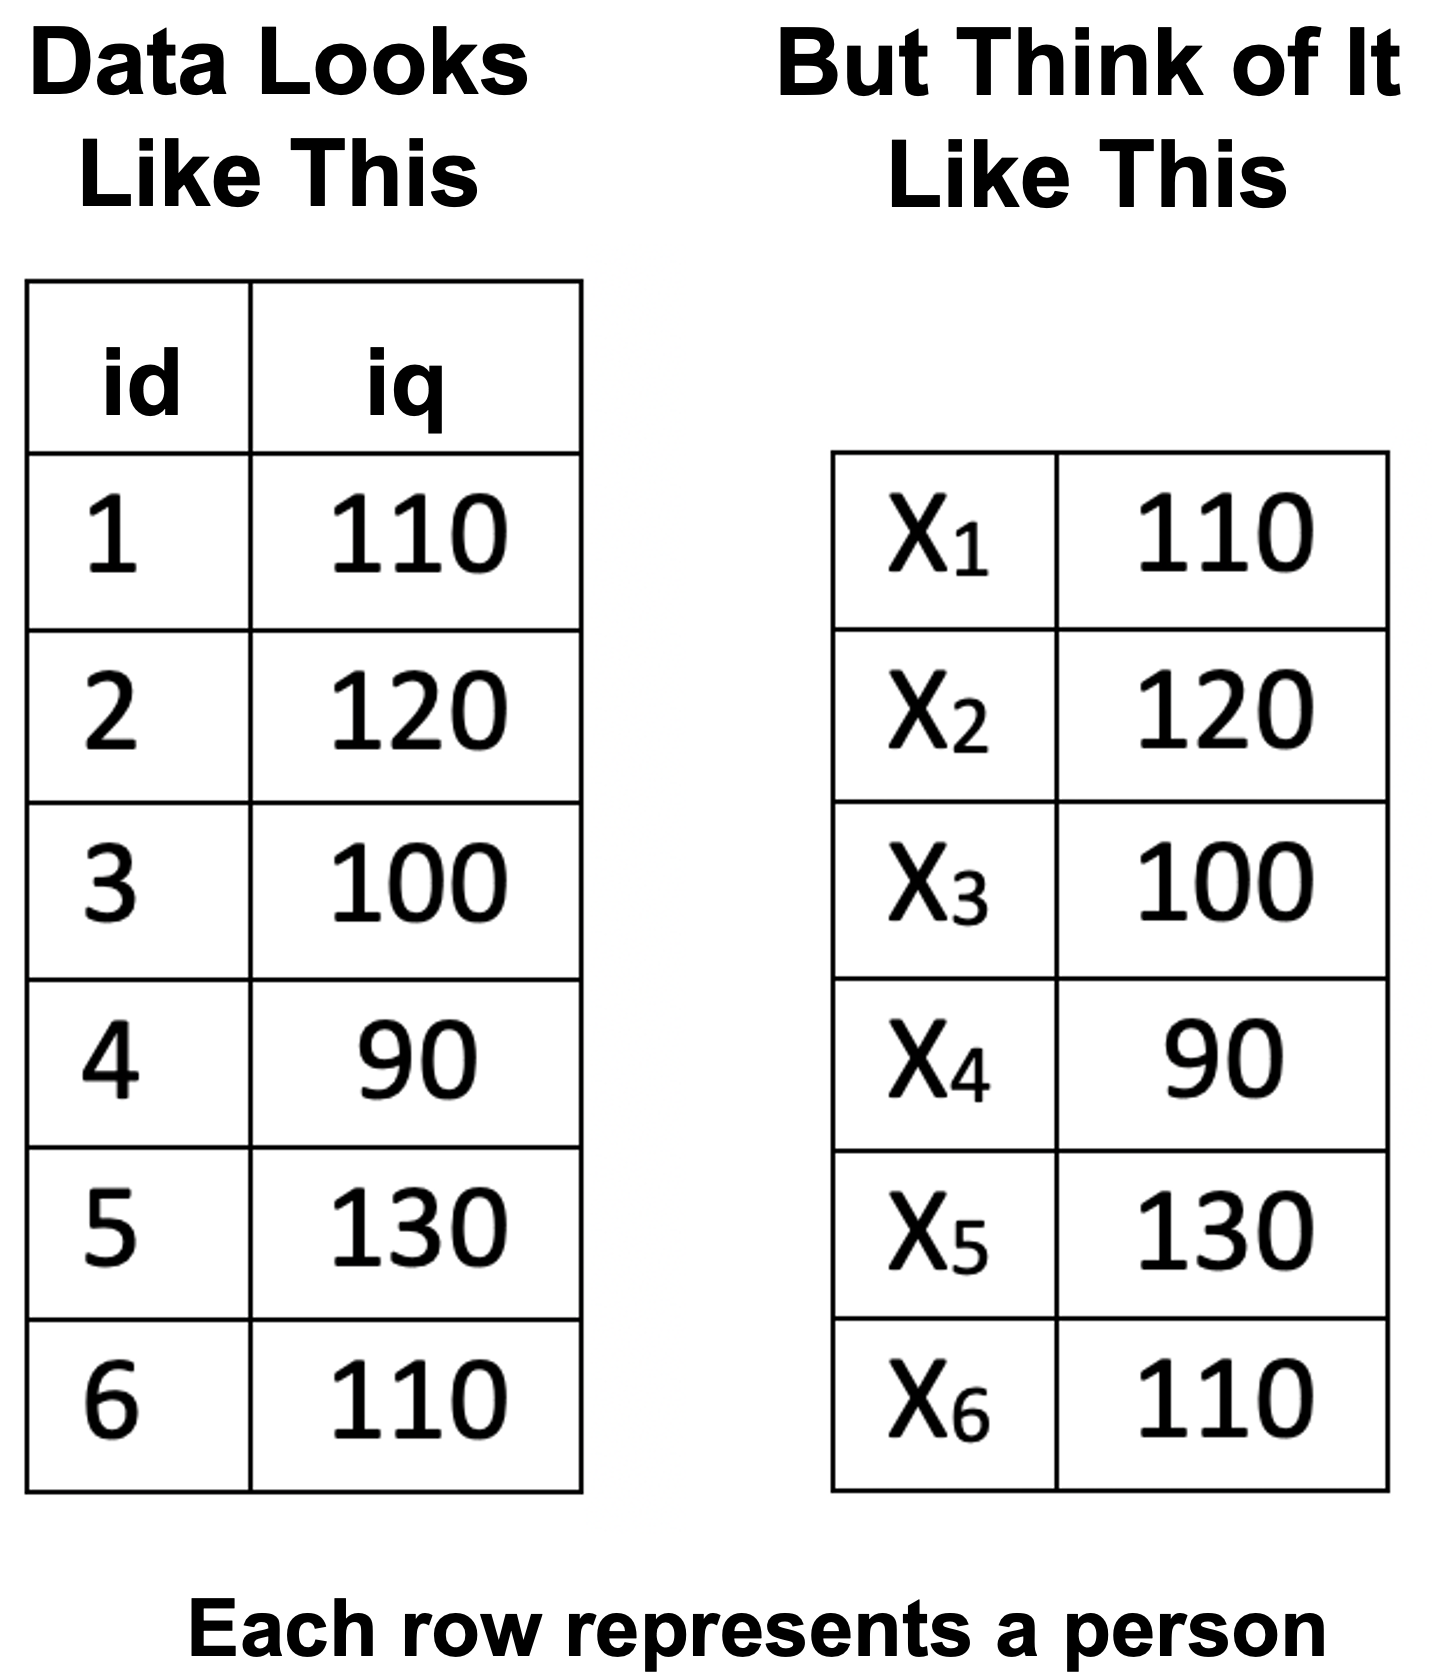
\includegraphics[width=0.4\linewidth]{ch_populations/images/screenshot_data_n6} \caption{Data for understanding summation notation}\label{fig:notationdata}
\end{figure}

Referring to participants using the variable X and subscript is valuable because it can be used in conjunction with the sigma (i.e., \(\Sigma\)) symbol for summation. Consider the example below in which we use the summation notation to indicate that we want to add all the X values (representing IQ) for the participants. We use a lower case \(i\) to represent all possible subscript values. The notation, \(i\) = 1, below the \(\Sigma\) symbol indicates that we should start with participant 1. The notation, N, above the \(\Sigma\) symbol indicates that we should iterate \(i\) up to the value indicated by N; in this case 3, because there are three participants.

\[
\begin{aligned} 
\sum_{i=1}^{N} X_i &=  X_1 + X_2 + X_3\\ 
&= 110 + 120 + 100 \\
&= 330
\end{aligned} 
\]

Sometimes, to simplify the notation, the numbers above and below the \(\Sigma\) symbol are omitted. Likewise, the \(i\) subscript is omitted. There is a general understanding that when these components of the notation are omitted the version of the notation above is implied.

\[
\begin{aligned} 
\sum{X} &= X_1 + X_2 + X_3\\ 
&= 110 + 120 + 100\\
&= 330
\end{aligned} 
\]

\textbf{Calculating a mean}. The full version of the notation can be used to indicate how an average/mean is calculated.

\[
\begin{aligned} 
\bar{X} &= \frac{\sum_{i=1}^{N} X_i}{N} \\
&= \frac{X_1 + X_2 + X_3}{3}\\ 
&= \frac{110 + 120 + 100}{3}\\
&= \frac{330}{3}\\
&= 110\\
\end{aligned} 
\]

Likewise, the concise version of the notation can be used to indicate how an average/mean is calculated.

\[
\begin{aligned} 
\bar{X} &= \frac{\sum{X}}{N} \\
&= \frac{X_1 + X_2 + X_3}{3}\\ 
&= \frac{110 + 120 + 100}{3}\\
&= \frac{330}{3}\\
&= 110\\
\end{aligned} 
\]

\textbf{Calculating squared differences}.A common task in statistics is to calculate 1) the squared difference between each person and the mean, and 2) add up those squared differences. This calculation is easily expressed with the full version of the notation.

\[
\begin{aligned} 
\sum_{i=1}^{N}{(X_i - \bar{X})^2} &= (X_1-\bar{X})^2 + (X_2-\bar{X})^2 + (X_3-\bar{X})^2\\ 
&= (110-110)^2 + (120-110)^2 + (100-110)^2\\
&= (0)^2 + (10)^2 (-10)^2 \\
&= 0 + 100 + 100 \\
&= 200
\end{aligned} 
\]

Likewise, the sum of the squared differences from the mean can be expressed using the concise version of the notation.

\[
\begin{aligned} 
\sum{(X - \bar{X})^2} &= (X_1-\bar{X})^2 + (X_2-\bar{X})^2 + (X_3-\bar{X})^2\\ 
&= (110-110)^2 + (120-110)^2 + (100-110)^2\\
&= (0)^2 + (10)^2 (-10)^2 \\
&= 0 + 100 + 100 \\
&= 200
\end{aligned} 
\]

\hypertarget{population-vs-samples}{%
\section{Population vs samples}\label{population-vs-samples}}

As we move closer to conducting our own research it is critical to make a distinction between populations and samples. A population is the complete set of people/animals about which we want to make conclusions. A sample is a randomly selected subset of the population. In most scenarios it is impractical to work with an entire population and, for practical reasons, we study a subset of the population called a sample.

Researchers, and consumers of research, typically have little interest in making conclusions at the sample level. In general, we care about conclusions that generalize to the population but not conclusions that only apply to specific individuals in the sample. Consider the case of COVID-19. Imagine a research team creates a vaccine that they hope generates immunity to COVID-19. We care very little if the immunity only works for the specific individuals in the study. However, we care a great deal if the immunity works, or is likely to work, for all Canadians or all humans. We study samples but typically wish to make conclusions that apply to the population. Thus, even if you are an experimental researcher it's critical that you think in terms of populations and not samples. Indeed, statistical tests (such as the \emph{t}-test) are a means of helping researchers use sample data to make conclusions at the population level.

In this chapter, our focus is on describing populations. When we calculate a number that summarises an attribute of all of the people/animals in the population we refer to it as a \textbf{parameter}.

\hypertarget{a-small-population}{%
\section{A small population}\label{a-small-population}}

In this section we review how to calculate three commonly used population parameters (mean, variance, and standard deviation). Populations are typically quite large but for simplicity we focus on a population composed of the weights of just three chocolate chip cookies. We refer to the three cookies as \(X_1\), \(X_2\), and \(X_3\). The cookies have the weights of 8, 10, and 12 grams, respectively.

\hypertarget{mean-mu}{%
\subsection{\texorpdfstring{Mean (\(\mu\))}{Mean (\textbackslash mu)}}\label{mean-mu}}

It can be helpful to create a model that describes our data. Of course, the model won't describe every participant perfectly and each participant will differ to some extent from the model.

\textbf{Model:} To create a model we first need data, which in this example will be the weight of three different chocolate chip cookies. As mentioned previously, the weights of the three cookies are designated by \(X_1\), \(X_2\), and \(X_3\). A simple model for our cookie weight data is the mean. At the population level the mean is represented by the symbol \(\mu\) see Formula \eqref{eq:popmeanch4} below. At the sample level a different notation is used.

\begin{equation} 
\mu = \frac{\sum{X}}{N}
      \label{eq:popmeanch4}
\end{equation}

Using that equation with values:

\[
\begin{aligned} 
\mu &= \frac{\sum{X}}{N} \\
&= \frac{X_1 + X_2 + X_3}{3}\\ 
&= \frac{8 + 10 + 12}{3}\\
&= \frac{30}{3}\\
&= 10\\
\end{aligned} 
\]

We can think of the ``mean cookie'' as our model for our cookie weight data, see Figure \ref{fig:meancookie}. The ``mean cookie'' is represented by \(\mu\) in equations.

\begin{figure}
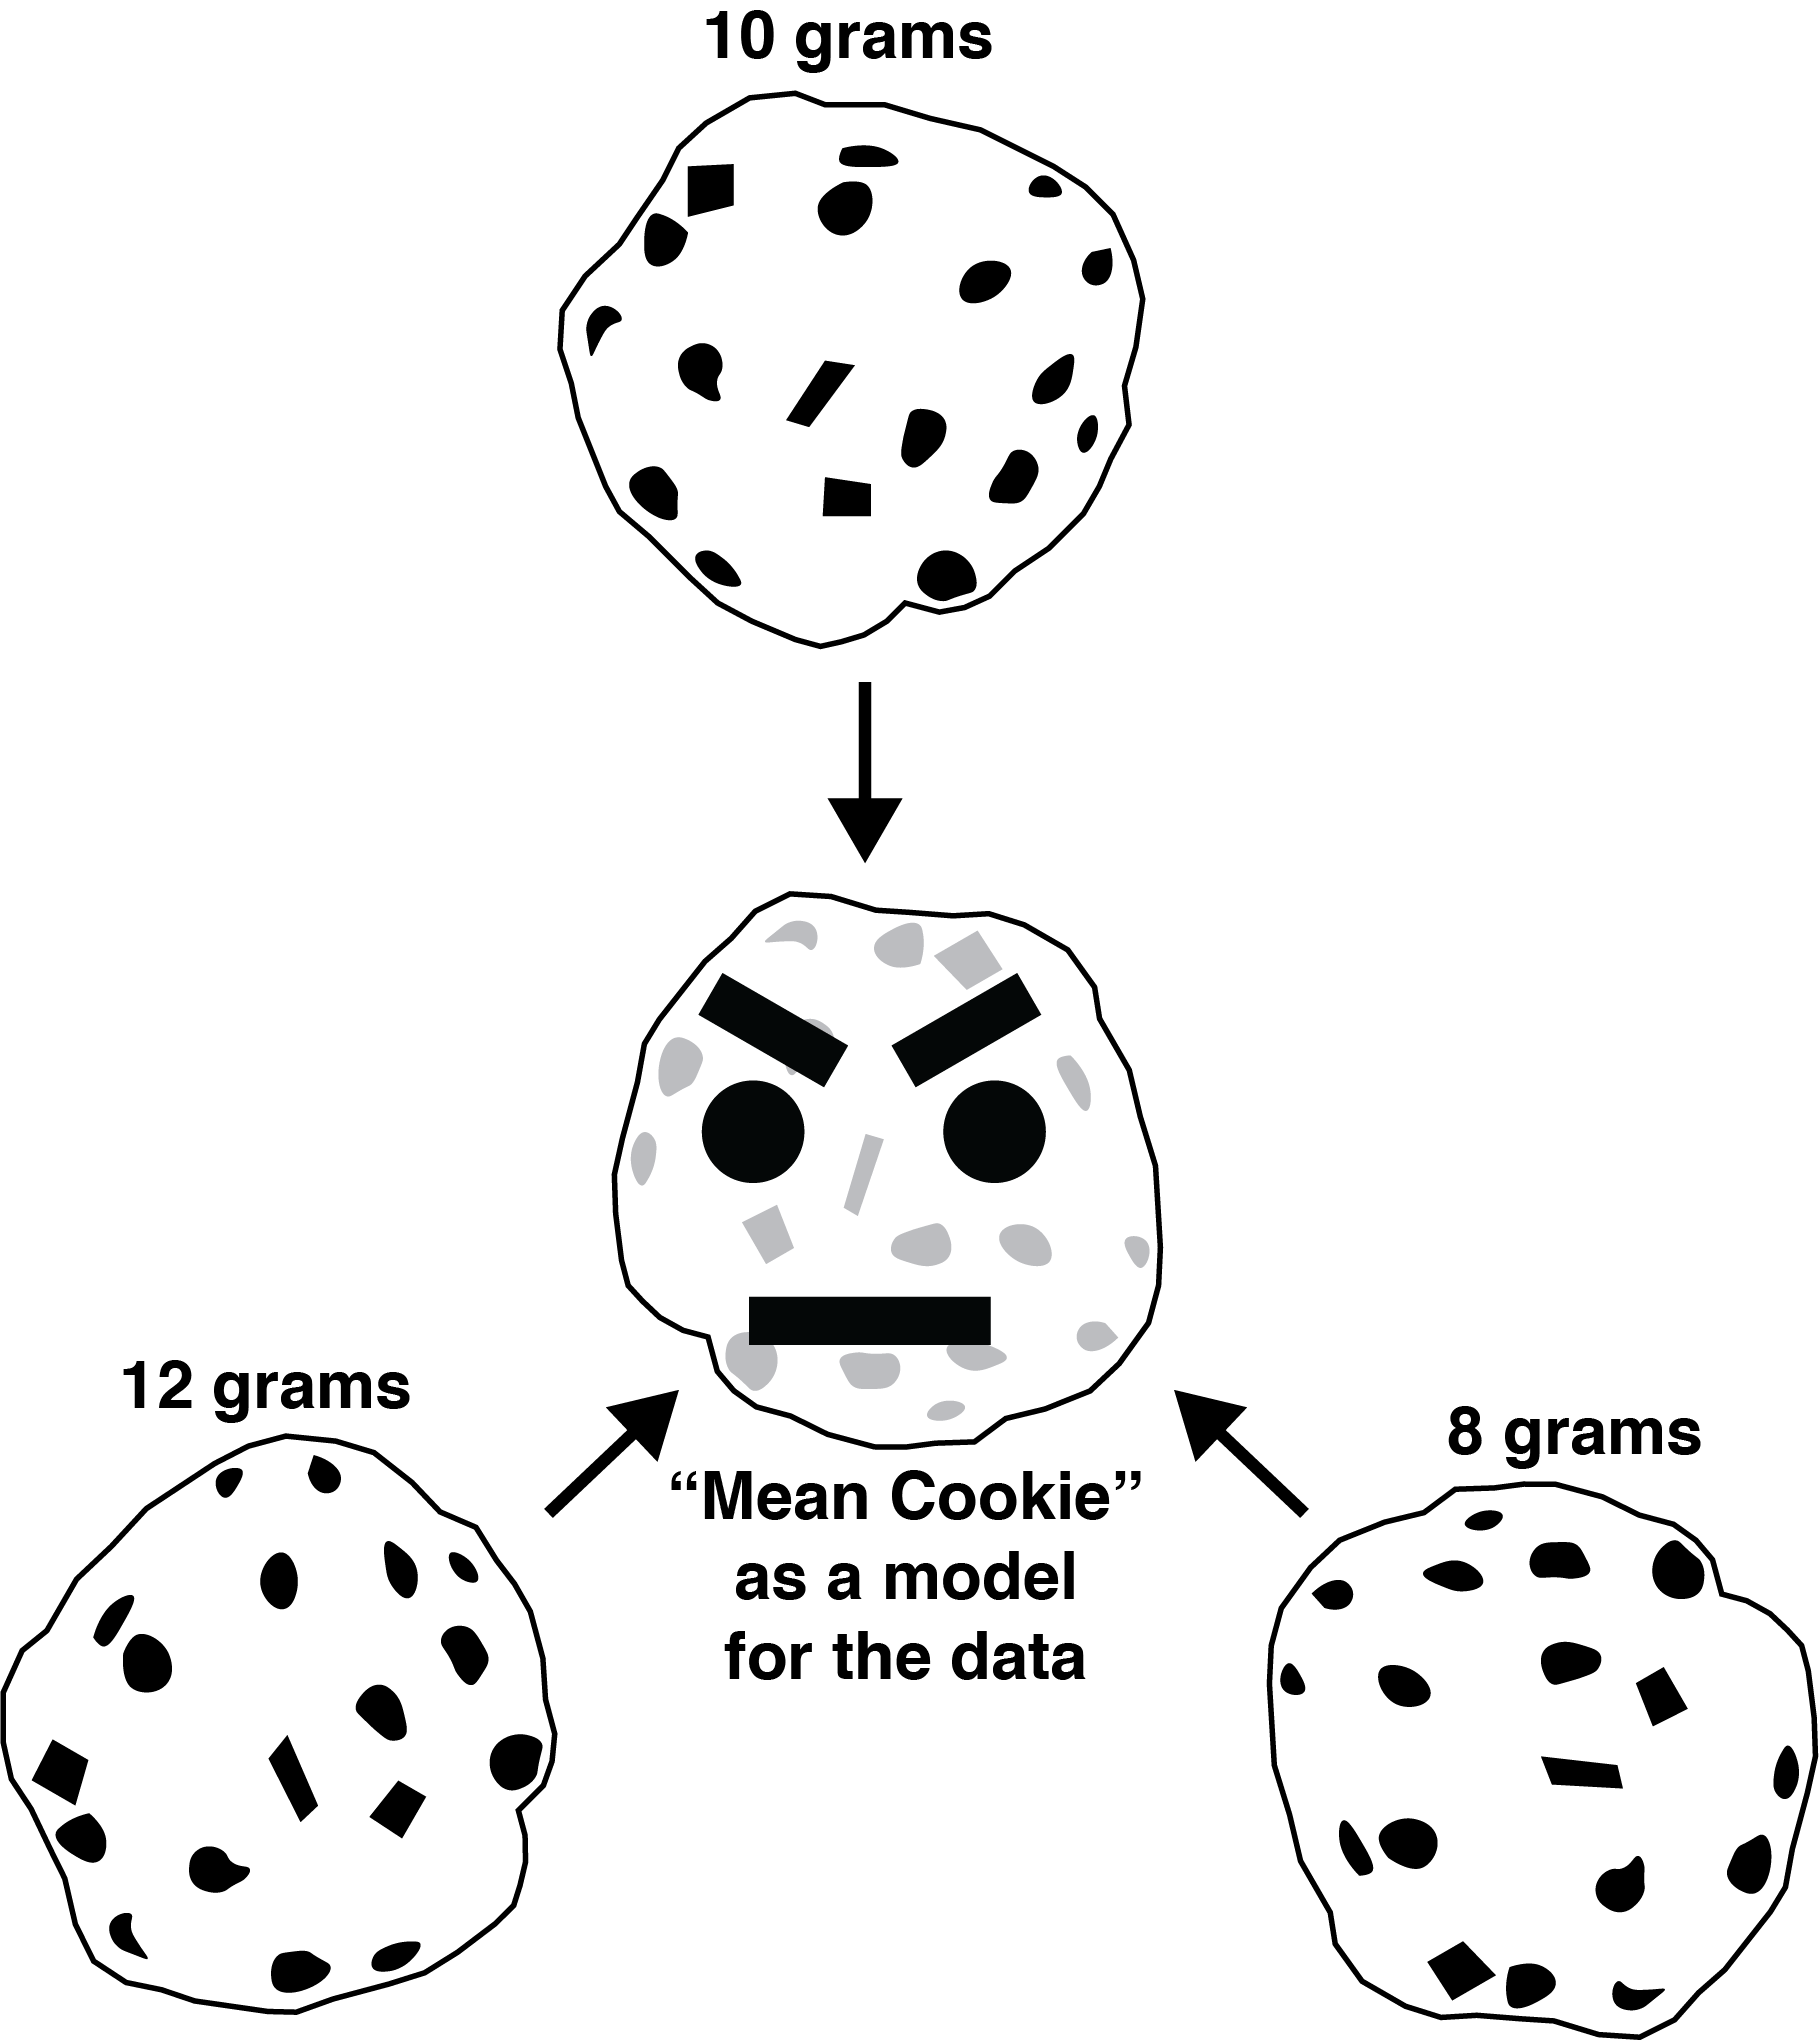
\includegraphics[width=0.6\linewidth]{ch_populations/images/cookie} \caption{Variance as a fit index for the mean}\label{fig:meancookie}
\end{figure}

\textbf{Error:} As mentioned previously, each participant (i.e., cookie) differs to some extent from our model (``mean cookie''). In general this can be conceptualized as:

\[
\begin{aligned} 
X_i &= model + error_i \\
\end{aligned} 
\]

More specifically, the difference between the weight of any individual cookie (\(X_i\)) and the model (\(\mu\)) is indicated by \(error_i\) as shown below.

\[
\begin{aligned} 
X_i &= \mu + error_i \\
\end{aligned} 
\]

The model, above is just a concise way of describing the following:

\[
\begin{aligned} 
X_1 &= \mu + error_1 \\
X_2 &= \mu + error_2 \\
X_3 &= \mu + error_3 \\
\end{aligned} 
\]

That is the weights of the three cookies (\(X_1 = 8\), \(X_2 = 10\), and \(X_3 = 12\)) can be conceptualized as:

\[
\begin{aligned} 
X_1 &= 10 + (-2) \\
X_2 &= 10 + 0 \\
X_3 &= 10 + 2 \\
\end{aligned} 
\]

The mean/average of the population, \(\mu = 10\), is a parameter that serves as a model for the cookie weight data. However, it's helpful to have an index, known as variance, that indicates the extent to which the data do not correspond to the model from the model.

\hypertarget{variance-sigma2}{%
\subsection{\texorpdfstring{Variance (\(\sigma^2\))}{Variance (\textbackslash sigma\^{}2)}}\label{variance-sigma2}}

Variance is a simple way of calculating a single number to represent how data differ from a model. It is represented, at the population level, by the symbol \(\sigma^2\); a different notation is used at the sample level.

Previously, how we expressed the difference/deviation of cookie weights (data) from the model (i.e., mean) with an error term in the equation \(X_i = \mu +error_i\), see see Figure \ref{fig:meancookie}. The model for all the cookies is \(\mu = 10\). If we consider a single cookie weight of 8 grams (a data point represented by \(X_1\)), the difference between the cookie from the model is -2 (i.e., error):

\[
\begin{aligned} 
X_1 &= 10 + (-2) \\
\end{aligned} 
\]

We want a number that indicates the quality of the cookie model. Specifically, we want a single number that indexes overall how the data (i.e., cookie weights) differ from the model (i.e., the mean cookie). We refer to that index as variance (\(\sigma^2\)).

\textbf{Calculating Squared Errors.} To calculate variance (\(\sigma^2\)), we use the errors for the cookies -- how the cookies differ from the mean/model. The first step is to square the errors/differnces. Those squared numbers are referred to as the ``squared differences'' or ``squared errors''. The calculation of the squared error for each cookie weight is shown below. The squared errors (or squared differences) are 4, 0, and 4.

\begin{longtable}[]{@{}lll@{}}
\toprule
Cookie Weight & Model & Squared Difference\tabularnewline
\midrule
\endhead
\(X_1 = 8\) & \(\mu = 10\) & \((X_1 - \mu)^2 =(8 - 10)^2= 4\)\tabularnewline
\(X_2 = 10\) & \(\mu = 10\) & \((X_2 - \mu)^2 =(10 - 10)^2= 0\)\tabularnewline
\(X_3 = 12\) & \(\mu = 10\) & \((X_3 - \mu)^2 =(12 - 10)^2= 4\)\tabularnewline
\bottomrule
\end{longtable}

\textbf{Averaging Squared Errors.} To obtain variance we calculate the average of the squared errors. At the population level the variance is represented by the symbol \(\sigma^2\) see Formula \eqref{eq:popvarch4} below. In this formula, \(N\) refers to the number of people in the population. At the sample level a different notation is used.

\begin{equation} 
\sigma^2 = \frac{\sum{(X - \mu)^2}}{N}
      \label{eq:popvarch4}
\end{equation}

Using that equation with values:

\[
\begin{aligned} 
\sigma^2 &= \frac{\sum{(X - \mu)^2}}{N}\\
&= \frac{(X_1-\mu)^2 + (X_2-\mu)^2 + (X_3-\mu)^2}{N}  \\ 
&= \frac{(8-10)^2 + (10-10)^2 + (12-10)^2}{3}\\
&= \frac{(-2)^2 + (0)^2 (2)^2}{3} \\
&= \frac{4 + 0 + 4}{3} \\
&= \frac{8}{3} \\
&= 2.67 grams^2 \\
\end{aligned} 
\]

The resulting variance is 2.67 grams\(^2\). The cookie weights were measured in grams. The unit for variance, however, is grams\(^2\) because we squared the errors as part of the calculation. Recall the formula for calculating an average (shown below) and compare it to the variance calculation (above). Notice that variance is just an average -- an average of squared errors. Correspondingly, in some areas of statistics they don't use the term variance, they use a synonym - \textbf{mean squared error}.

\[
\begin{aligned} 
\bar{X} &= \frac{\sum{X}}{N} \\
\end{aligned} 
\]

It probably strikes you as an odd choice to square the difference between each data point and the model. Why not just use the difference (e.g., \((8 - 10) = -2\)) when calculating variance? Why not use the absolute difference (e.g., \(|8 - 10|= 2\)) when calculating variance? The answer is somewhat complex, but it relates to the more general situation in statistics of trying to find models that best fit the data (which occurs by minimizing errors). When we use squared errors it is easier to apply calculus, via derivatives, to calculate a model that minimizes the errors (i.e., obtains the best fit). Long story short, for complex mathematical reasons, we use squared errors when calculating the fit (or lack of fit) of a model.

\textbf{Interpretation}. A variance of zero indicates that the model fits the data perfectly. In the cookie case, if the variance was zero, that would indicate that all the cookies had the same weight as the model, exactly 10 grams. To the extent that the variance is larger than zero it implies the data points (i.e., cookie weights) differ from the model (i.e., the mean cookie). By implication, a larger variance indicates larger differences among the observations (e.g., cookie weights). That is, when the variance is small, cookie weights tend to be similar to the model -- and each other. In contrast, when the variance is large, cookie weights tend to be different from the model -- and each other.

\hypertarget{standard-deviation-sigma}{%
\subsection{\texorpdfstring{Standard Deviation (\(\sigma\))}{Standard Deviation (\textbackslash sigma)}}\label{standard-deviation-sigma}}

An alternative index for how data differ from the mean/model is the standard deviation. To understand standard deviation you have to understand varince. Variance is a single number that indexes how data differ from a model. The interpretation of variance is straight forward. It is the average of the squared differences between the data and the model.

Standard deviation is represented by the symbol \(\sigma\) and can be calculated as the square root of variance as in Formula \eqref{eq:popsdch4} below.

\begin{equation} 
\sigma = \sqrt{\frac{\sum{(X - \mu)^2}}{N}}
      \label{eq:popsdch4}
\end{equation}

Using that equation with values:

\[
\begin{aligned} 
\sigma &= \sqrt{\frac{\sum{(X - \mu)^2}}{N}}\\
&= \sqrt{\sigma^2} \\
&= \sqrt{2.67} \\
&= 1.63 grams\\
\end{aligned} 
\]

One reason that people like standard deviation is presents the difference between the data and the model in the original units (e.g., grams). This is in contrast to variance which presents the difference betweeen the data and the model in squared units (e.g., 2.67 grams\(^2\)).

\textbf{Interpretation}. Unfortunately, although variance has a straight forward interpretation, standard deviation does not. Sometimes standard deviation is, incorrectly, described as how much data points differ on average from the mean. A quick calculation of the average difference reveals a number (1.33) that does not correspond to the standard deviation (1.63):

\[
\begin{aligned} 
\overline{diff} &= \frac{\sum{|X - \mu|}}{N}\\
&= \frac{|8-10| + |10-10| + |12 - 10|}{3}\\
&= \frac{2 + 0 + 2}{3}\\
&= \frac{4}{3}\\
&= 1.33\\
\end{aligned} 
\]

As illustrated above, standard deviation is not equal to the average of the deviations from the mean. Because standard deviation is not an average, it's much harder to describe how to interpret it. In our view, the best way to think of standard deviation is simply as the square root of variance; because variance has a straight forward interpretation.

Therefore, we encourage you to think primarily in terms of variance rather than standard deviation due to the fact the interpretation of variance is more straightforward. Additionally, variance is foundational in the language used to describe regression and analysis of variance. That said, standard deviation is used in the calculation of some standardized effect sizes - so it is important to know and understand both indices.

Overall, the rules for interpreting standard deviation are similar to those for variance; but the standard deviation values are smaller than variance values. In the cookie case, if the standard deviation was zero, that would indicate that all the cookies had the same weight as the model, exactly 10 grams. To the extent that the standard deviation is larger than zero it implies the data points (i.e., cookie weights) differ from the model (i.e., the mean cookie). By implication, a larger standard deviation indicates larger differences among the observations (e.g., cookie weights). That is, when the standard deviation is small, cookie weights tend to be similar to the model -- and each other. In contrast, when the standard deviation is large, cookie weights tend to be different from the model -- and each other.

\hypertarget{visualizing-populations}{%
\section{Visualizing populations}\label{visualizing-populations}}

Populations are typically quite large in nature and it's often imposssible to pratically list all of the members of the population. Consequently, it helps to have ways to visual the entire population. In Figure \ref{fig:popvisual3} we present three ways of visualizing a population. In all three graphs (A, B, C) in this figure the x-axis represents heights in centimeter and the y-axis is used to indicate which values on the x-axis are more common. In Figure \ref{fig:popvisual3}A we use a large number of X's to indicate the members of the population. Because X's are also used in formulas to represent individual participants a strength of this graph is that it reminds you that it is a graph reflecting a large number of individuals. In Figure \ref{fig:popvisual3}B we present a standard histogram that illustrate the distribution of heights. In Figure \ref{fig:popvisual3}C we present a density curve that illustrate the distribution of heights. All three approaches are useful for illustrating that most people have heights around 170 cm.

\begin{figure}
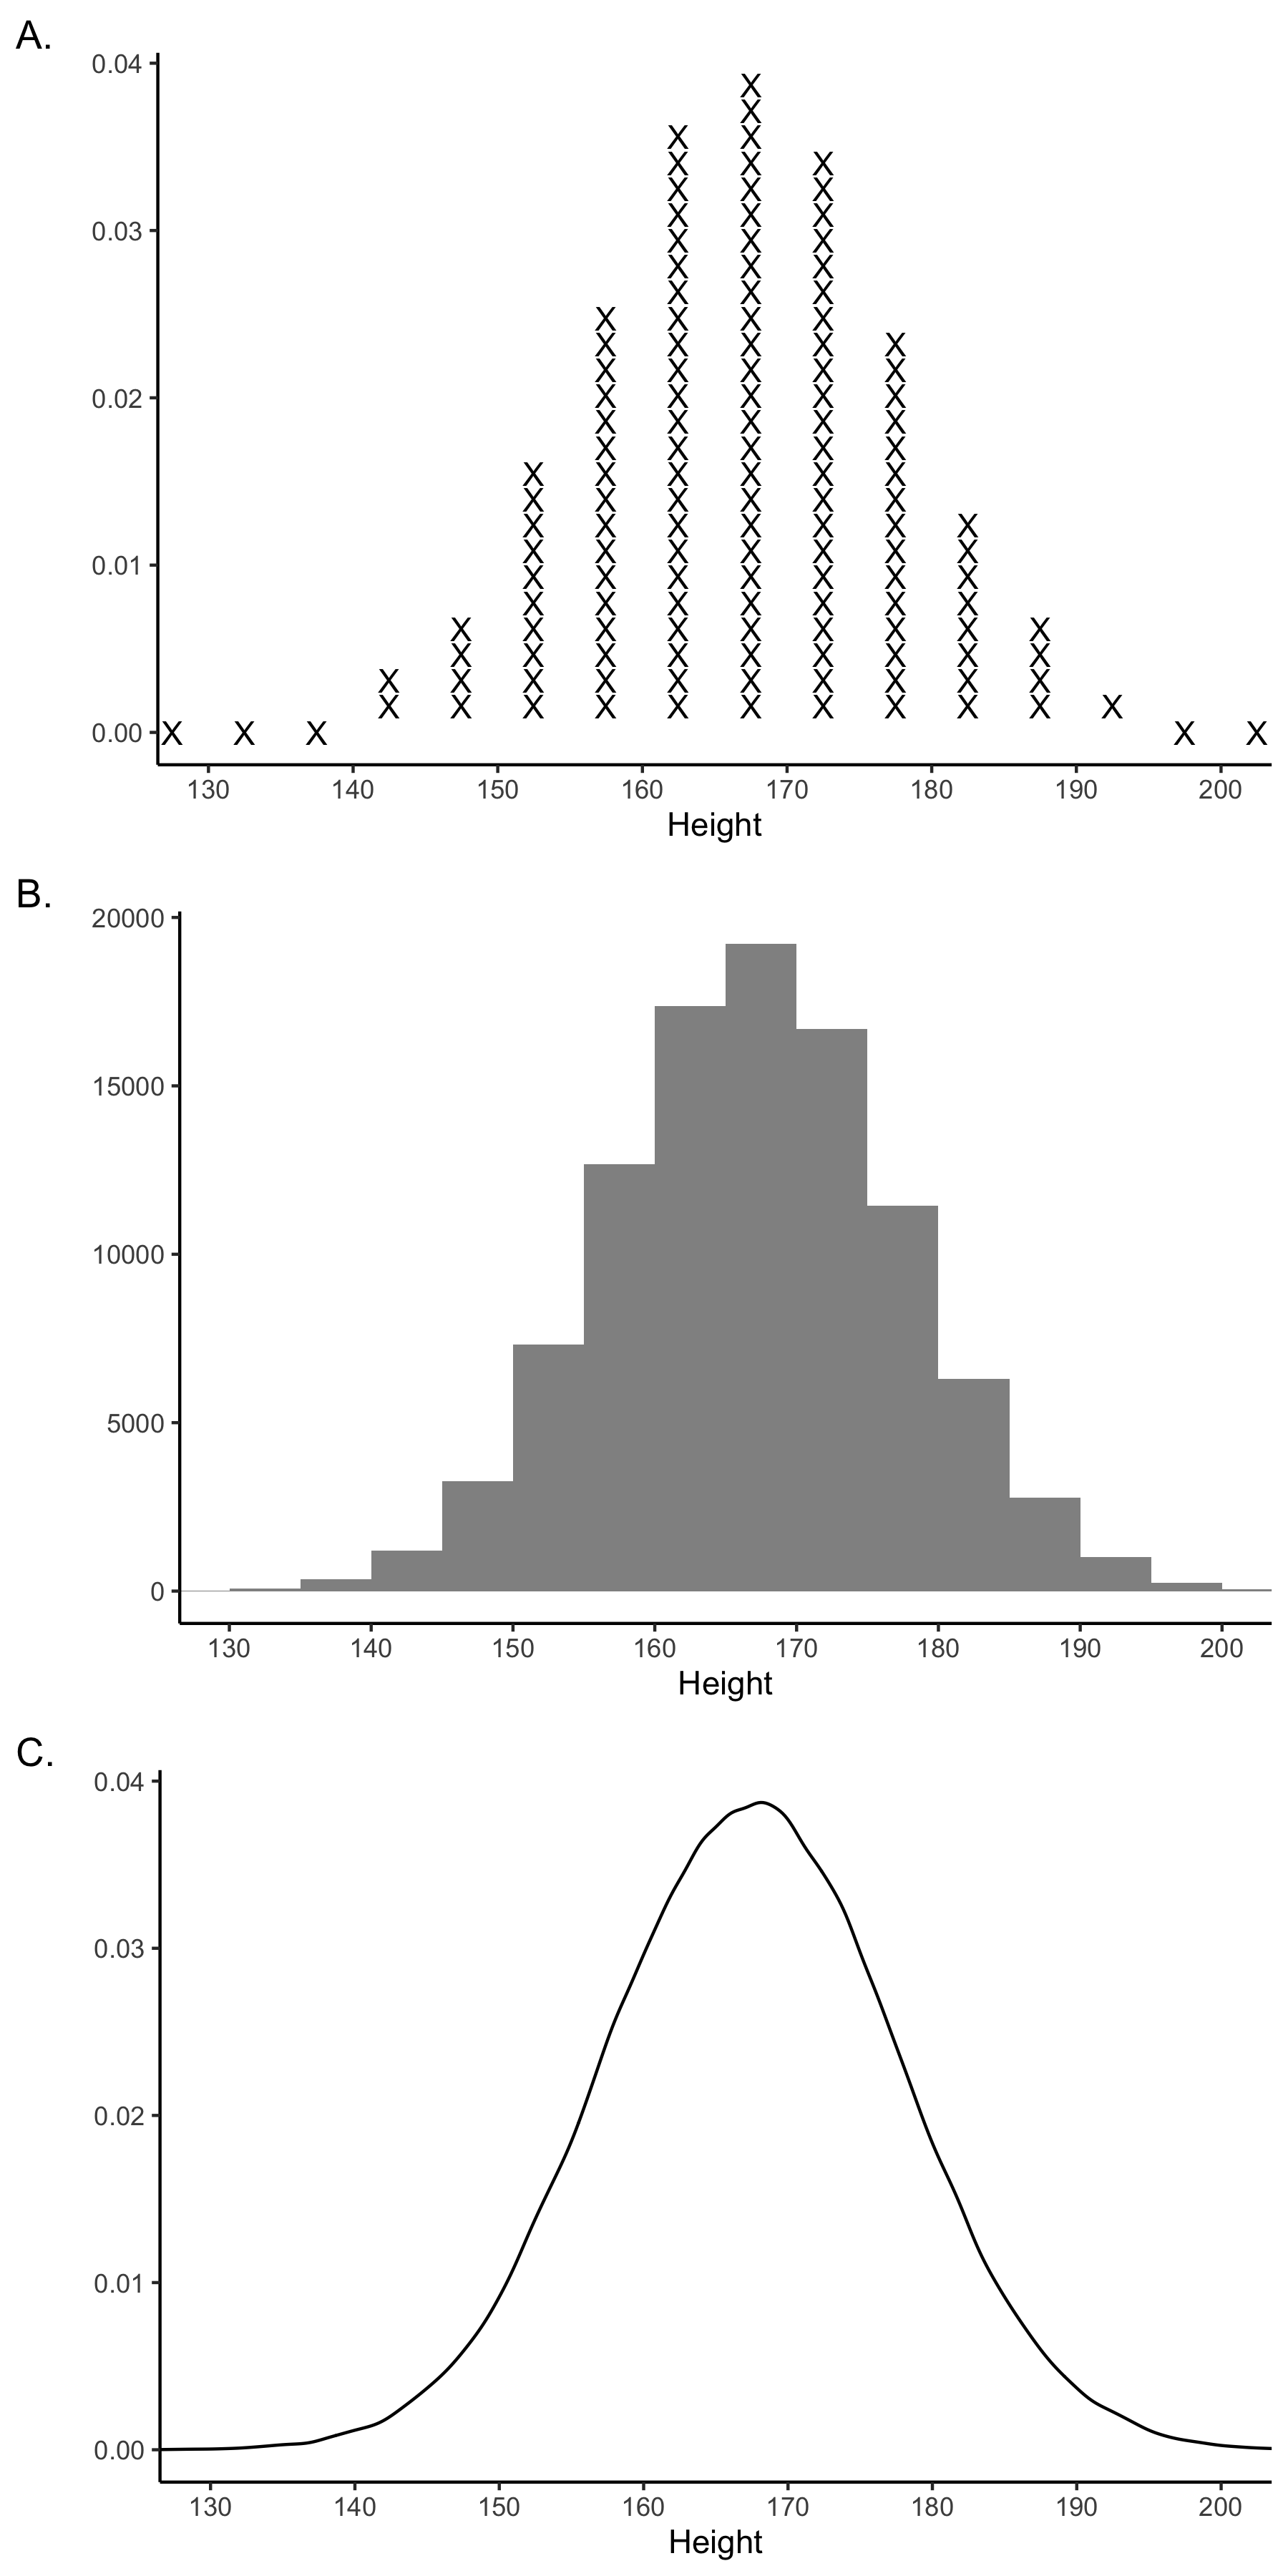
\includegraphics[width=0.8\linewidth,height=0.8\textheight]{ch_populations/images/popvisual} \caption{Three ways of visualizing a population distribution}\label{fig:popvisual3}
\end{figure}

\hypertarget{comparisons-same-sigma}{%
\section{\texorpdfstring{Comparisons: Same \(\sigma\)}{Comparisons: Same \textbackslash sigma}}\label{comparisons-same-sigma}}

In this section we review a method of comparing two population means when the populations have the same standard deviation. To facilitate comparing two populations we use the heights of males and females, measured in centimeters, as an example. On average males are taller than females. There is, however, variability in the heights of both males and females. The variability in heights is the same for males and females even though the means differ. We illustrate these differences in a series of figures below. Each figure contains three scenarios (labeled A, B, C) in which we manipulate the mean height and variability of the populations. In each scenario the standard deviation of heights is the same for the male and female populations.

\hypertarget{standardized-units}{%
\subsection{Standardized units}\label{standardized-units}}

\hypertarget{individual-scores}{%
\subsubsection{Individual scores}\label{individual-scores}}

Often when we compare two means we use the original metric. In the case of the male and female heights that metric is centimeters. The original units are a useful way to convey information about the difference between two populations.

In addition to the original unit it is also possible, and sometimes desirable, to use the standardized mean difference. The word \emph{standardized} is used to indicate that the comparison is relative to the standard deviation.

Imagine a population of male heights (\(\mu = 170\), \(\sigma = 10\)) from which we have obtained a single individual, Ian, whose height is 185 cm.

\[
X_{Ian} = 185cm
\]

The original units are useful for describing Ian's height but it doesn't tell us about his height relative to the other people in the population. We have to know the mean and standard deviation of the population to know if Ian is shorter or taller than the average height - and by how much. We use a \(z\)-score calculation for this purpose:

\[
\begin{aligned} 
z_{Ian} &=  \frac{X_{Ian} - \mu_{males}}{\sigma_{males}}\\ 
&=  \frac{185 - 170}{10}\\
&=  \frac{15}{10}\\
&= 1.50
\end{aligned} 
\]

The above calculation is a ratio. Ratios are used to compare two numbers. The numerator (number on the top) is compared to the denominator (number on bottom) through division. The resulting number tells you how much larger the numerator is than the denominator.

In this case, the numerator is the extent to which Ian is taller than the mean height for males (\(X_{Ian} - \mu_{males}\)). This numerator is compared to the denominator -- which is the standard deviation for males (\(\sigma_{males}\)). The resulting number is 1.50 which indicates the numerator is 1.50 times larger than the denominator. In other words, Ian is 1.50 standard deviations taller than the average male. This is a standardized score for Ian's height - it expresses the difference between his height and the mean height in standard deviation units.

\hypertarget{independent-group-population-means}{%
\subsubsection{Independent Group: Population Means}\label{independent-group-population-means}}

The same approach to generating standardized scores can be applied to population means. Consider a situation where we have population of male heights (\(\mu = 170\), \(\sigma = 10\)) and a population of female heights (\(\mu = 165\), \(\sigma = 10\)). Notice that both populations have the same standard deviation.

We can calculate a standardized value to compare these heights. This standardized value is called the standardized mean difference (SMD). Alternatively, it is also known as Cohen's \(d\) which is represented at the population level with the symbol \(\delta\). Calculation of the standardized mean difference is based on the premise that both populations have the same standard deviation.

In this calculation the numerator represents the difference between the two population means. The denominator represents the population standard deviation - which is the same for both populations see Formula \eqref{eq:popsmdch4} below.

\begin{equation} 
\delta =  \frac{\mu_{1} - \mu_{2}}{\sigma}
      \label{eq:popsmdch4}
\end{equation}

Using that equation with values:

\[
\begin{aligned} 
\delta &=  \frac{\mu_{males} - \mu_{females}}{\sigma}\\ 
&=  \frac{170 - 165}{10}\\
&=  \frac{5}{10}\\
&= 0.50
\end{aligned} 
\]

The resulting division of this ratio reveals that the numerator is 0.50 times as large (i.e., half as large) as the denominator. That is, the difference between the populations is half as large as the standard deviation. Therefore, the population mean for males is 0.50 standard deviations larger than the population mean for female; \(\delta = 0.50\):

\hypertarget{cohens-d-units}{%
\subsection{\texorpdfstring{Cohen's \(d\) units}{Cohen's d units}}\label{cohens-d-units}}

Because the unit for the standardized mean difference is the standard deviation it can be easy to interpret if you are unfamiliar with the original units. It is usually a good idea to report the difference between populations in both the original units (cm) and standardized units (\(\delta\)). Figure \ref{fig:dex1} illustrates three different population difference scenarios (A through C). The population standard deviation is held constant across the three scenarios. You can see that as the difference between the population means increases in raw units - it does the same in \(\delta\) (i.e., Cohen's \(d\)) units. In raw units (i.e., cm), the difference between the population means for scenarios A through C are 5 cm, 10 cm, and 20 cm, respectively. In standardized units (i.e., standard deviations), the difference the between the population means for scenarios A through C are 0.50 standard deviations, 1.0 standard deviations, and 2.0 standard deviations, respectively. In other words, the population-level Cohen's \(d\)-values are 0.50, 1.0, and 2.0 for scenarios A through C.

\begin{figure}
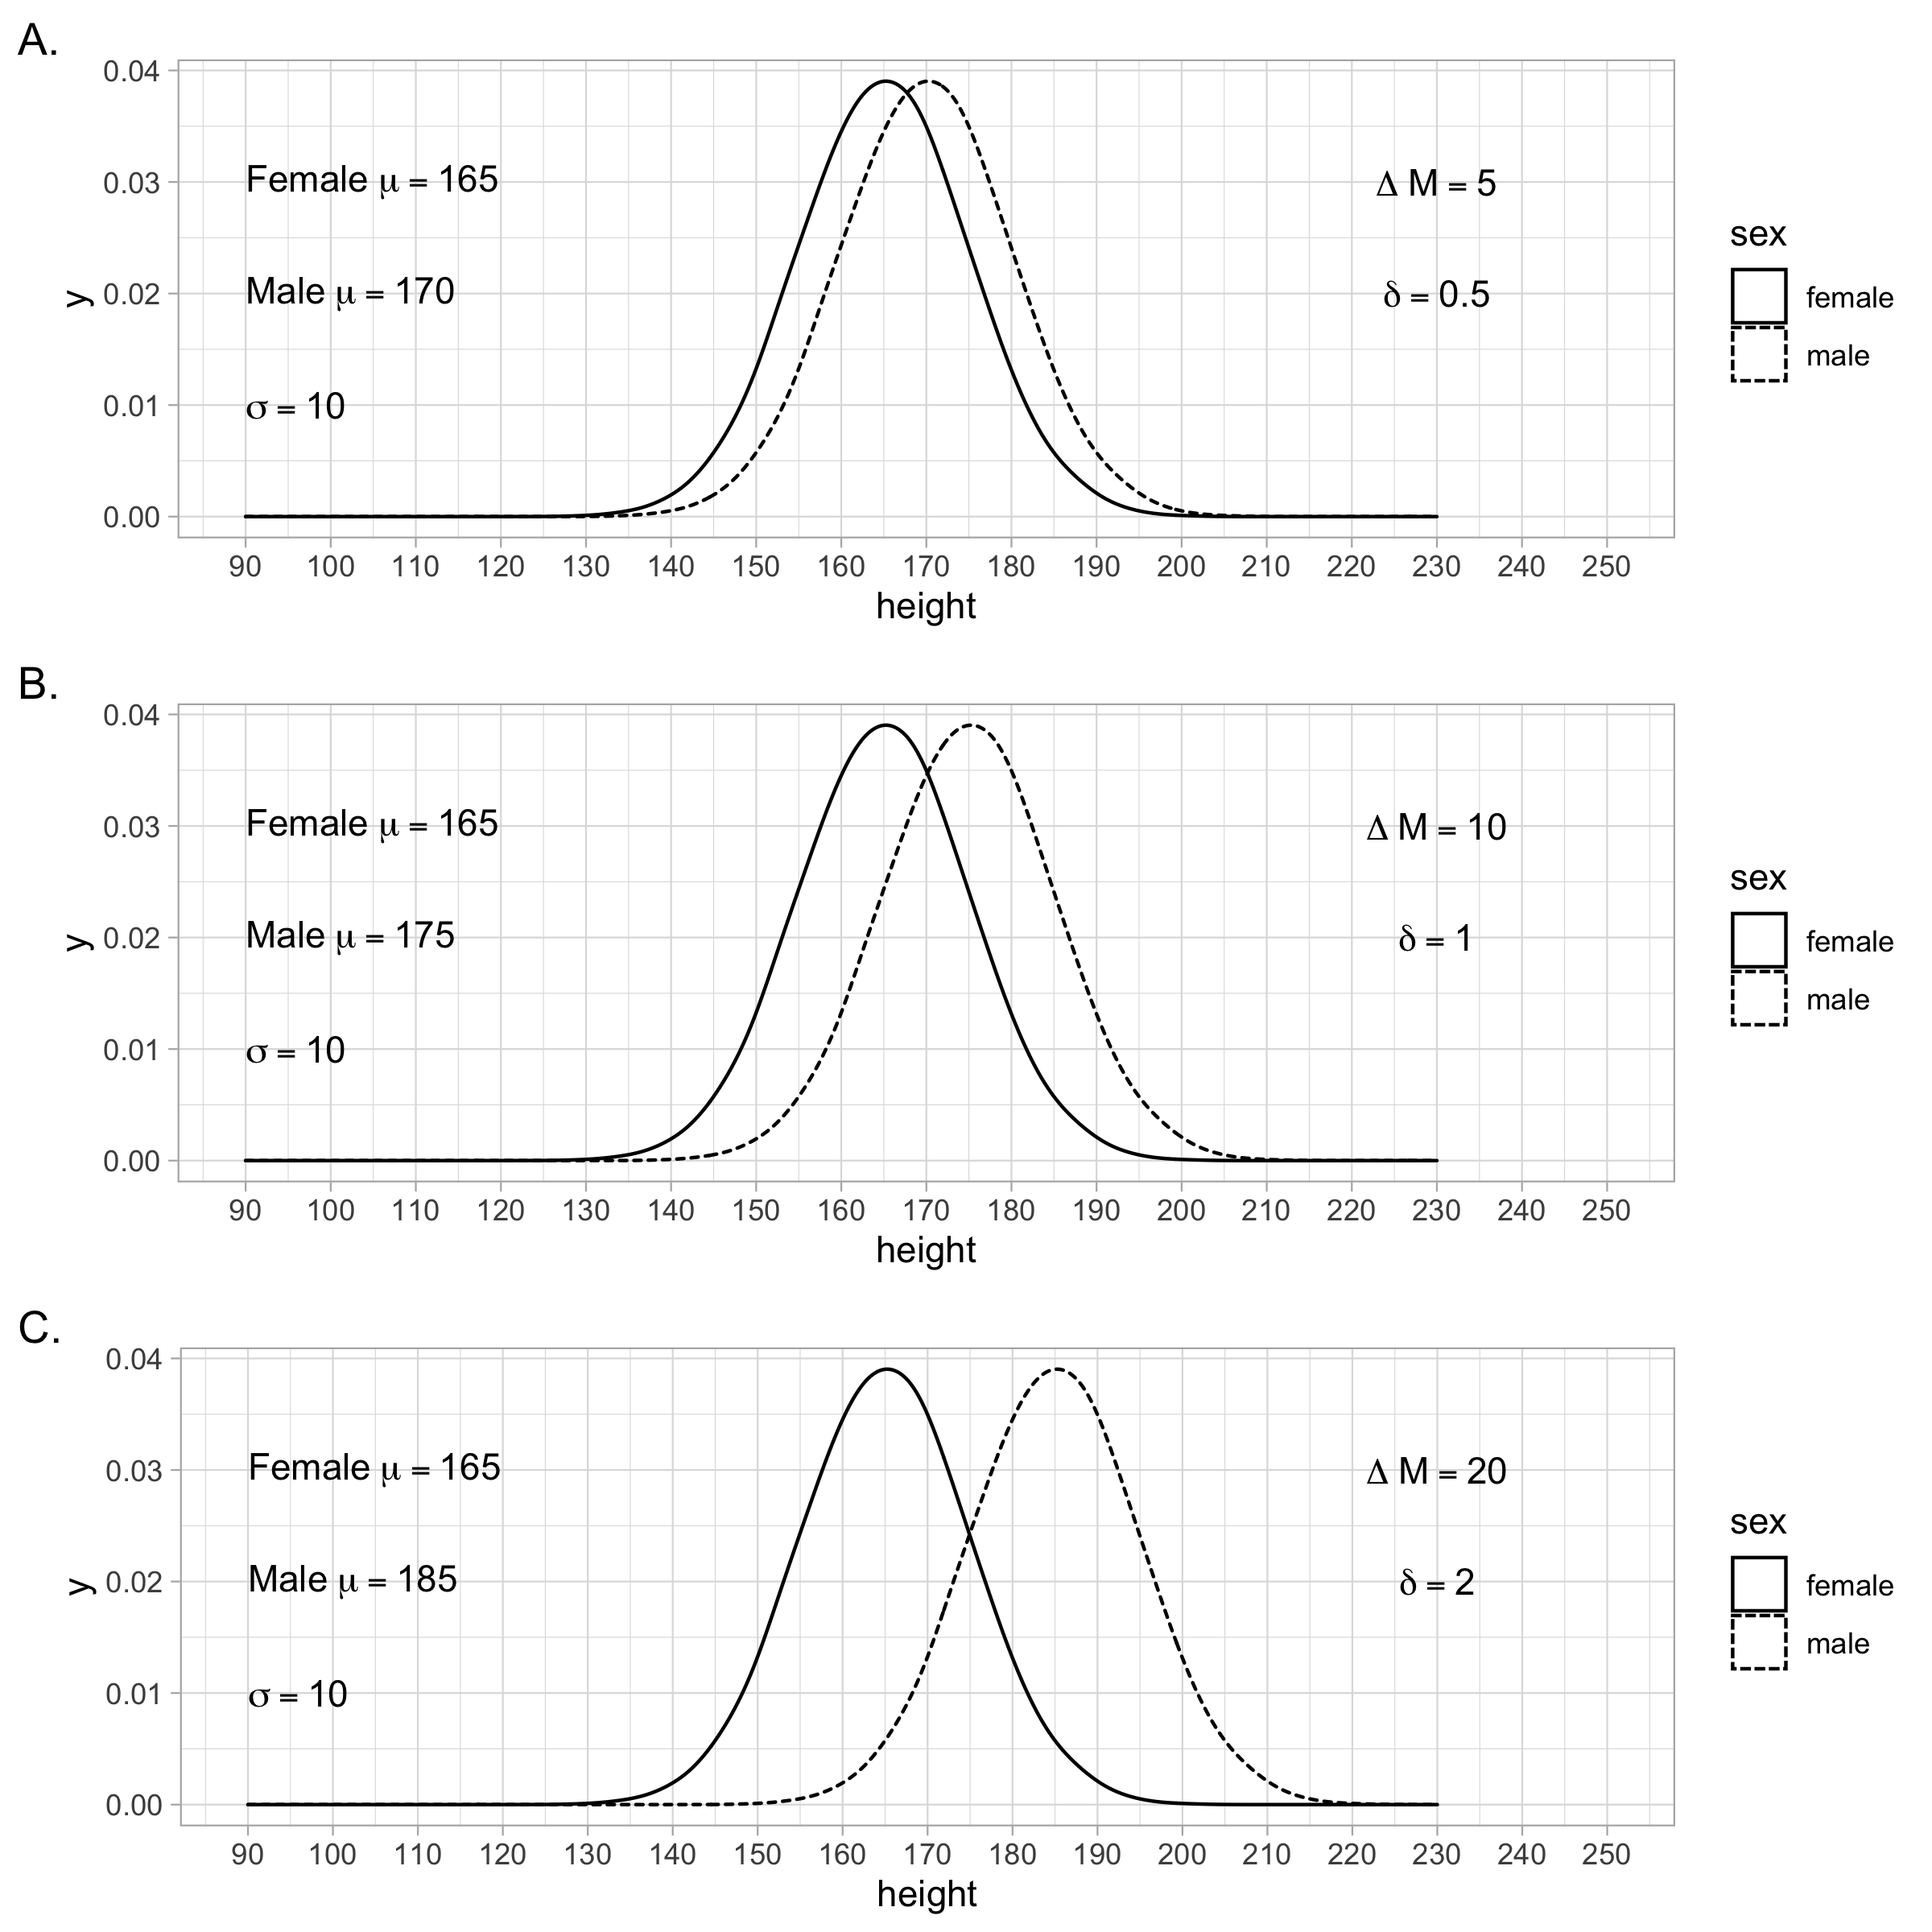
\includegraphics[width=1\linewidth]{ch_populations/images/dvalue_ex1} \caption[Illustrating standardized mean difference]{The difference between two population means can be expressed in the original units as indicated by $\Delta M$. Alternatively, the difference can be expressed using a Standardized Mean Difference (SMD). The SMD index is also known as the population-level $d$-value and is represented by the symbol $\delta$. The SMD is a way of expressing the difference between population means without using the original units. }\label{fig:dex1}
\end{figure}

\hypertarget{cohens-d-advantages}{%
\subsection{\texorpdfstring{Cohen's \(d\) advantages}{Cohen's d advantages}}\label{cohens-d-advantages}}

The standardized mean difference takes into account the variability of heights around each population mean. This means that the same difference between two population means can produce different standardized mean difference values if the population standard deviation varies. In the scenarios depicted in Figure \ref{fig:dex2} the population standard deviation becomes increasing small - resulting in larger standardized mean difference values (i.e., \(\delta\)). This larger \(\delta\) value corresponds to progressively less overlap between the two populations. Thus, taking into account the standard deviation of the populations can be viewed as a strength of using the standardized mean difference.

\begin{figure}
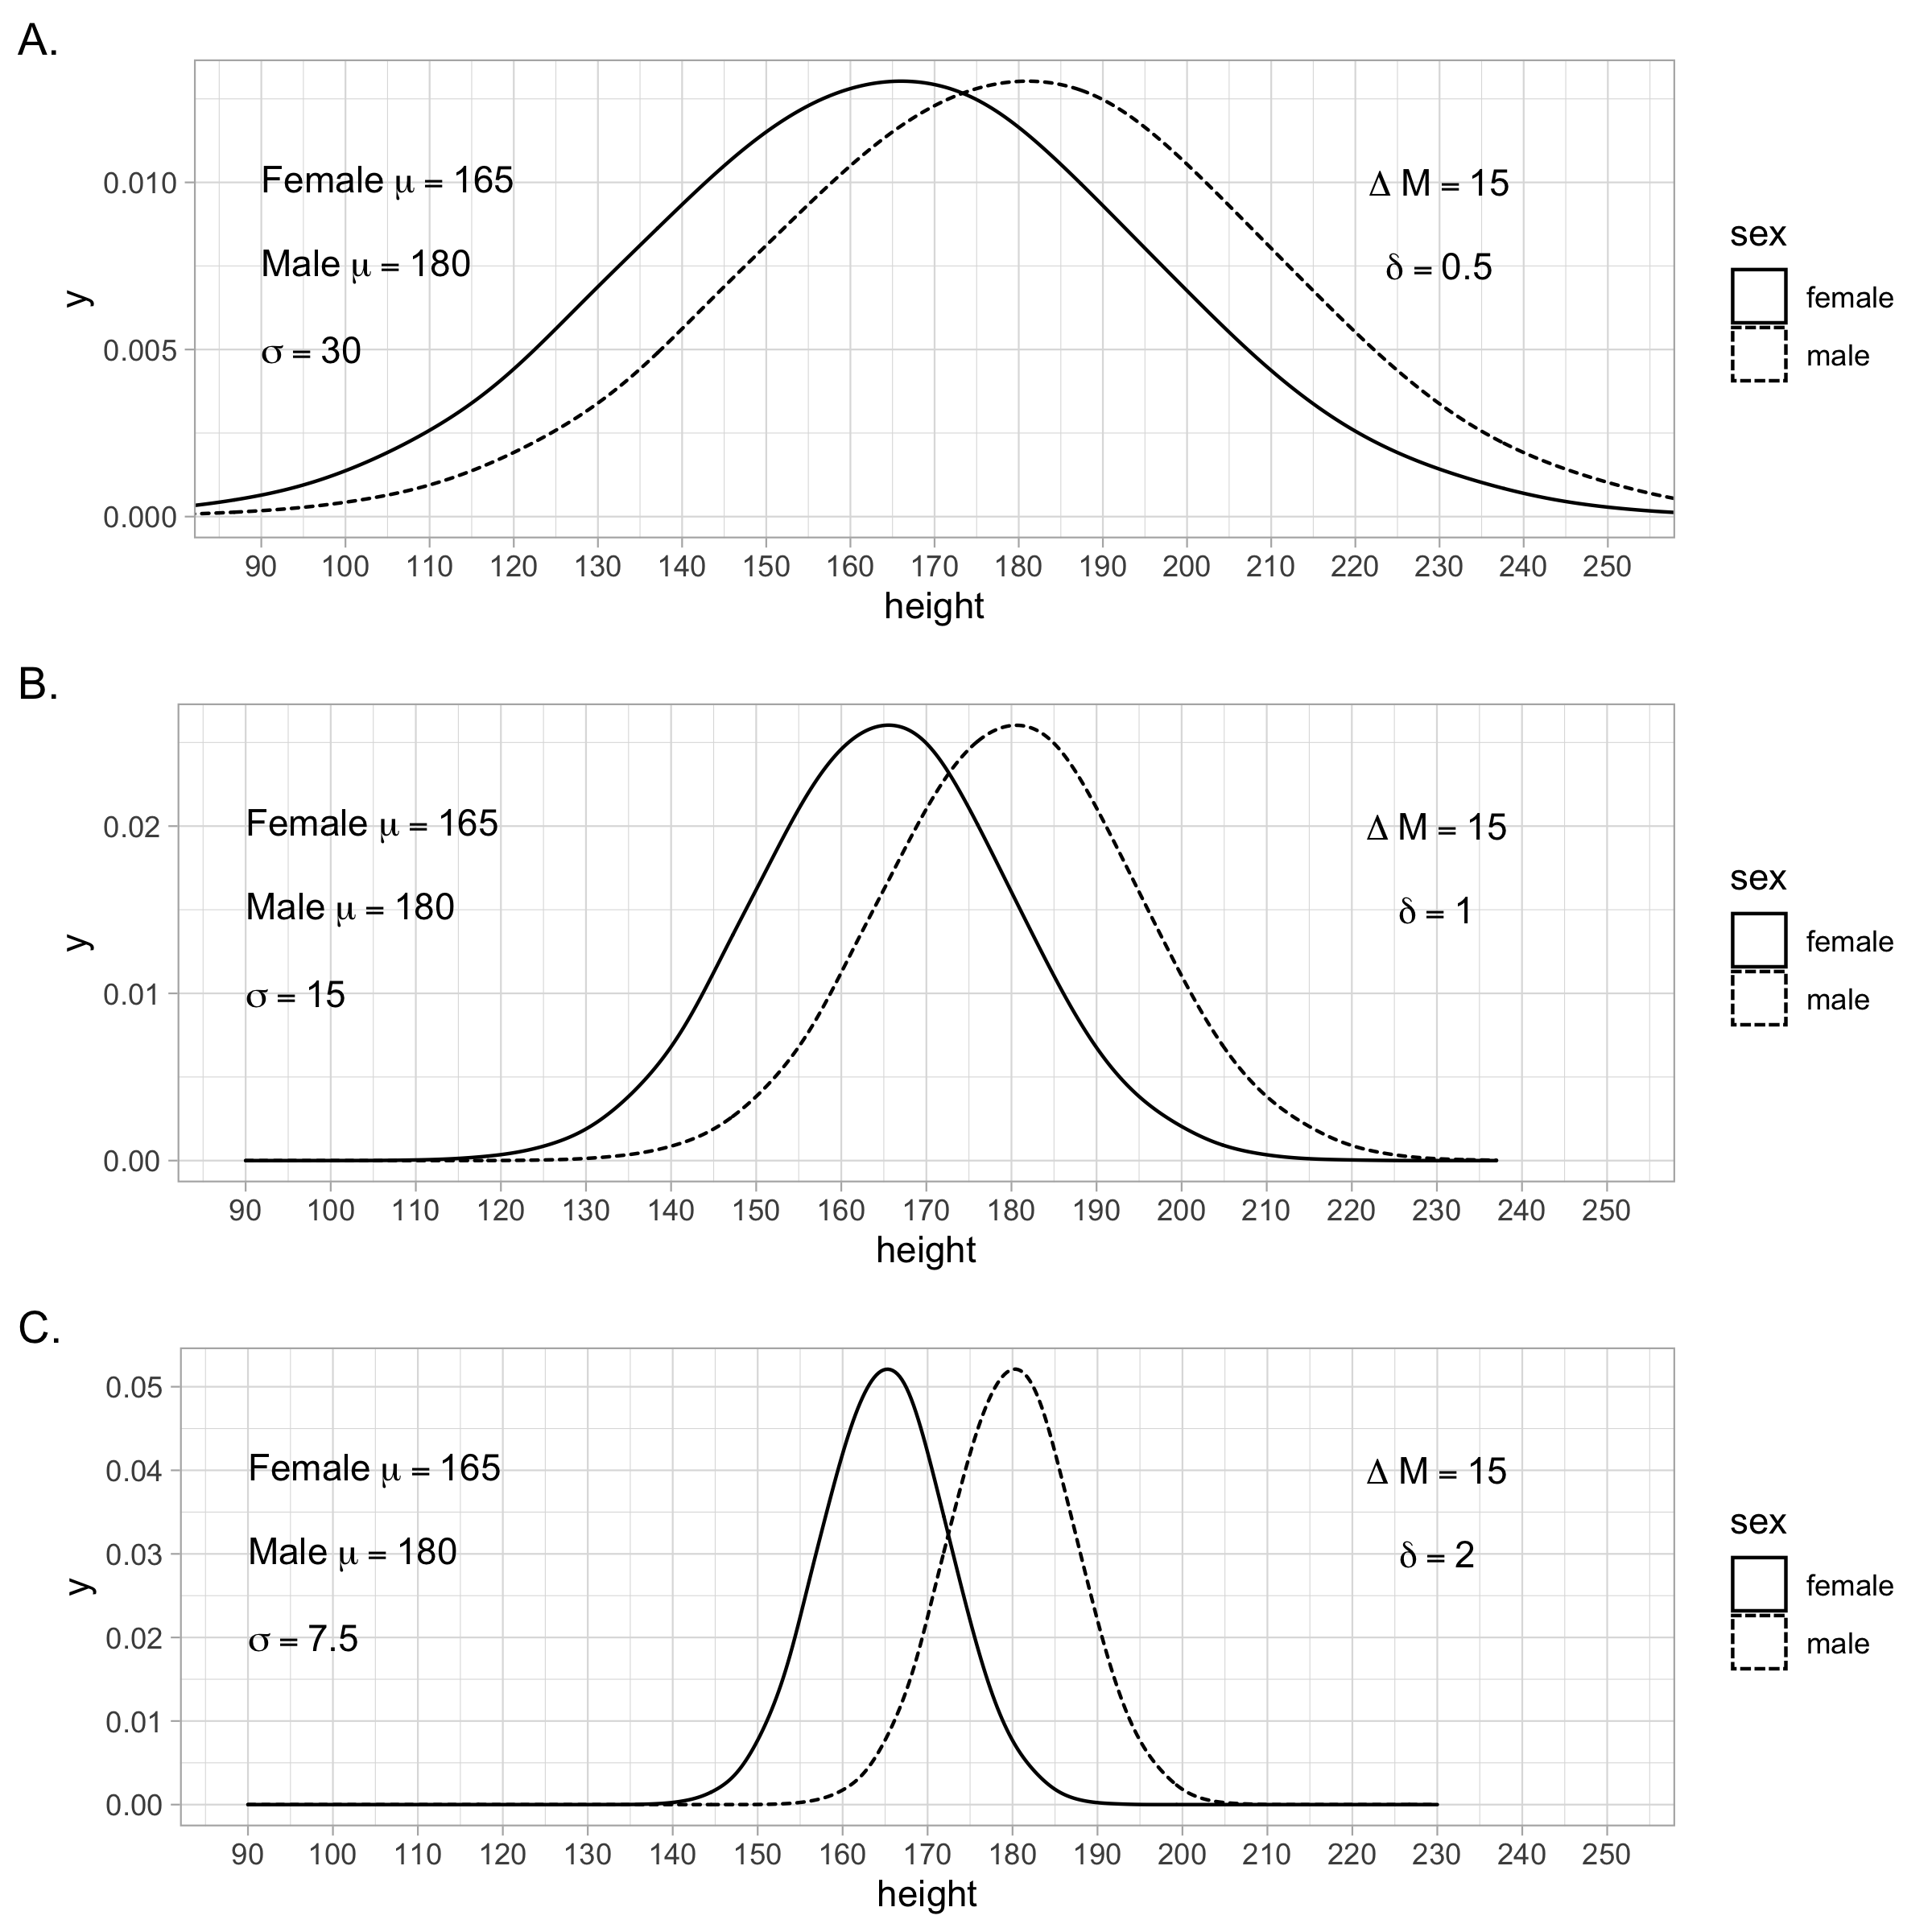
\includegraphics[width=1\linewidth]{ch_populations/images/dvalue_ex2} \caption[Advantages of standadized mean difference]{An advantage of using the Standardized Mean Difference (SMD) to index the difference between two population means (i.e., $\delta$) is that it takes the population standard deviation into account. In these three examples, the difference between the populations means is the same using the original/raw units of centimeters. However, the standard deviation of the populations varies across scenarios A, B, and C. The SMD illustrates that these three scenarios are different. If you only examined the difference in the original units (i.e., $\Delta M$) you would conclude the effect is the same across the three scenarios. However, by using SMD, indexed by $\delta$ - the population $d$-value, you see that the effect is progressively stronger from scenario A, to B, to C. This is illustrated by the fact that there is progressively less overlap between the distributions as you move from scenario A to C.}\label{fig:dex2}
\end{figure}

\hypertarget{cohens-d-caveats}{%
\subsection{\texorpdfstring{Cohen's \(d\) caveats}{Cohen's d caveats}}\label{cohens-d-caveats}}

It is important to also look at the original units when interpreting results - not just the standardized mean difference. Examine the scenarios in Figure \ref{fig:dex3}. Notice how the \(\delta\) value stays constant across scenarios - as does the overlap of the two distributions. However, inspect the shape of the curves and the original units to see how the scenarios vary. Both the original units and the standardized mean difference (i.e., Cohen's \(d\)) provide important interpretational information - don't rely on just one of them.

\begin{figure}
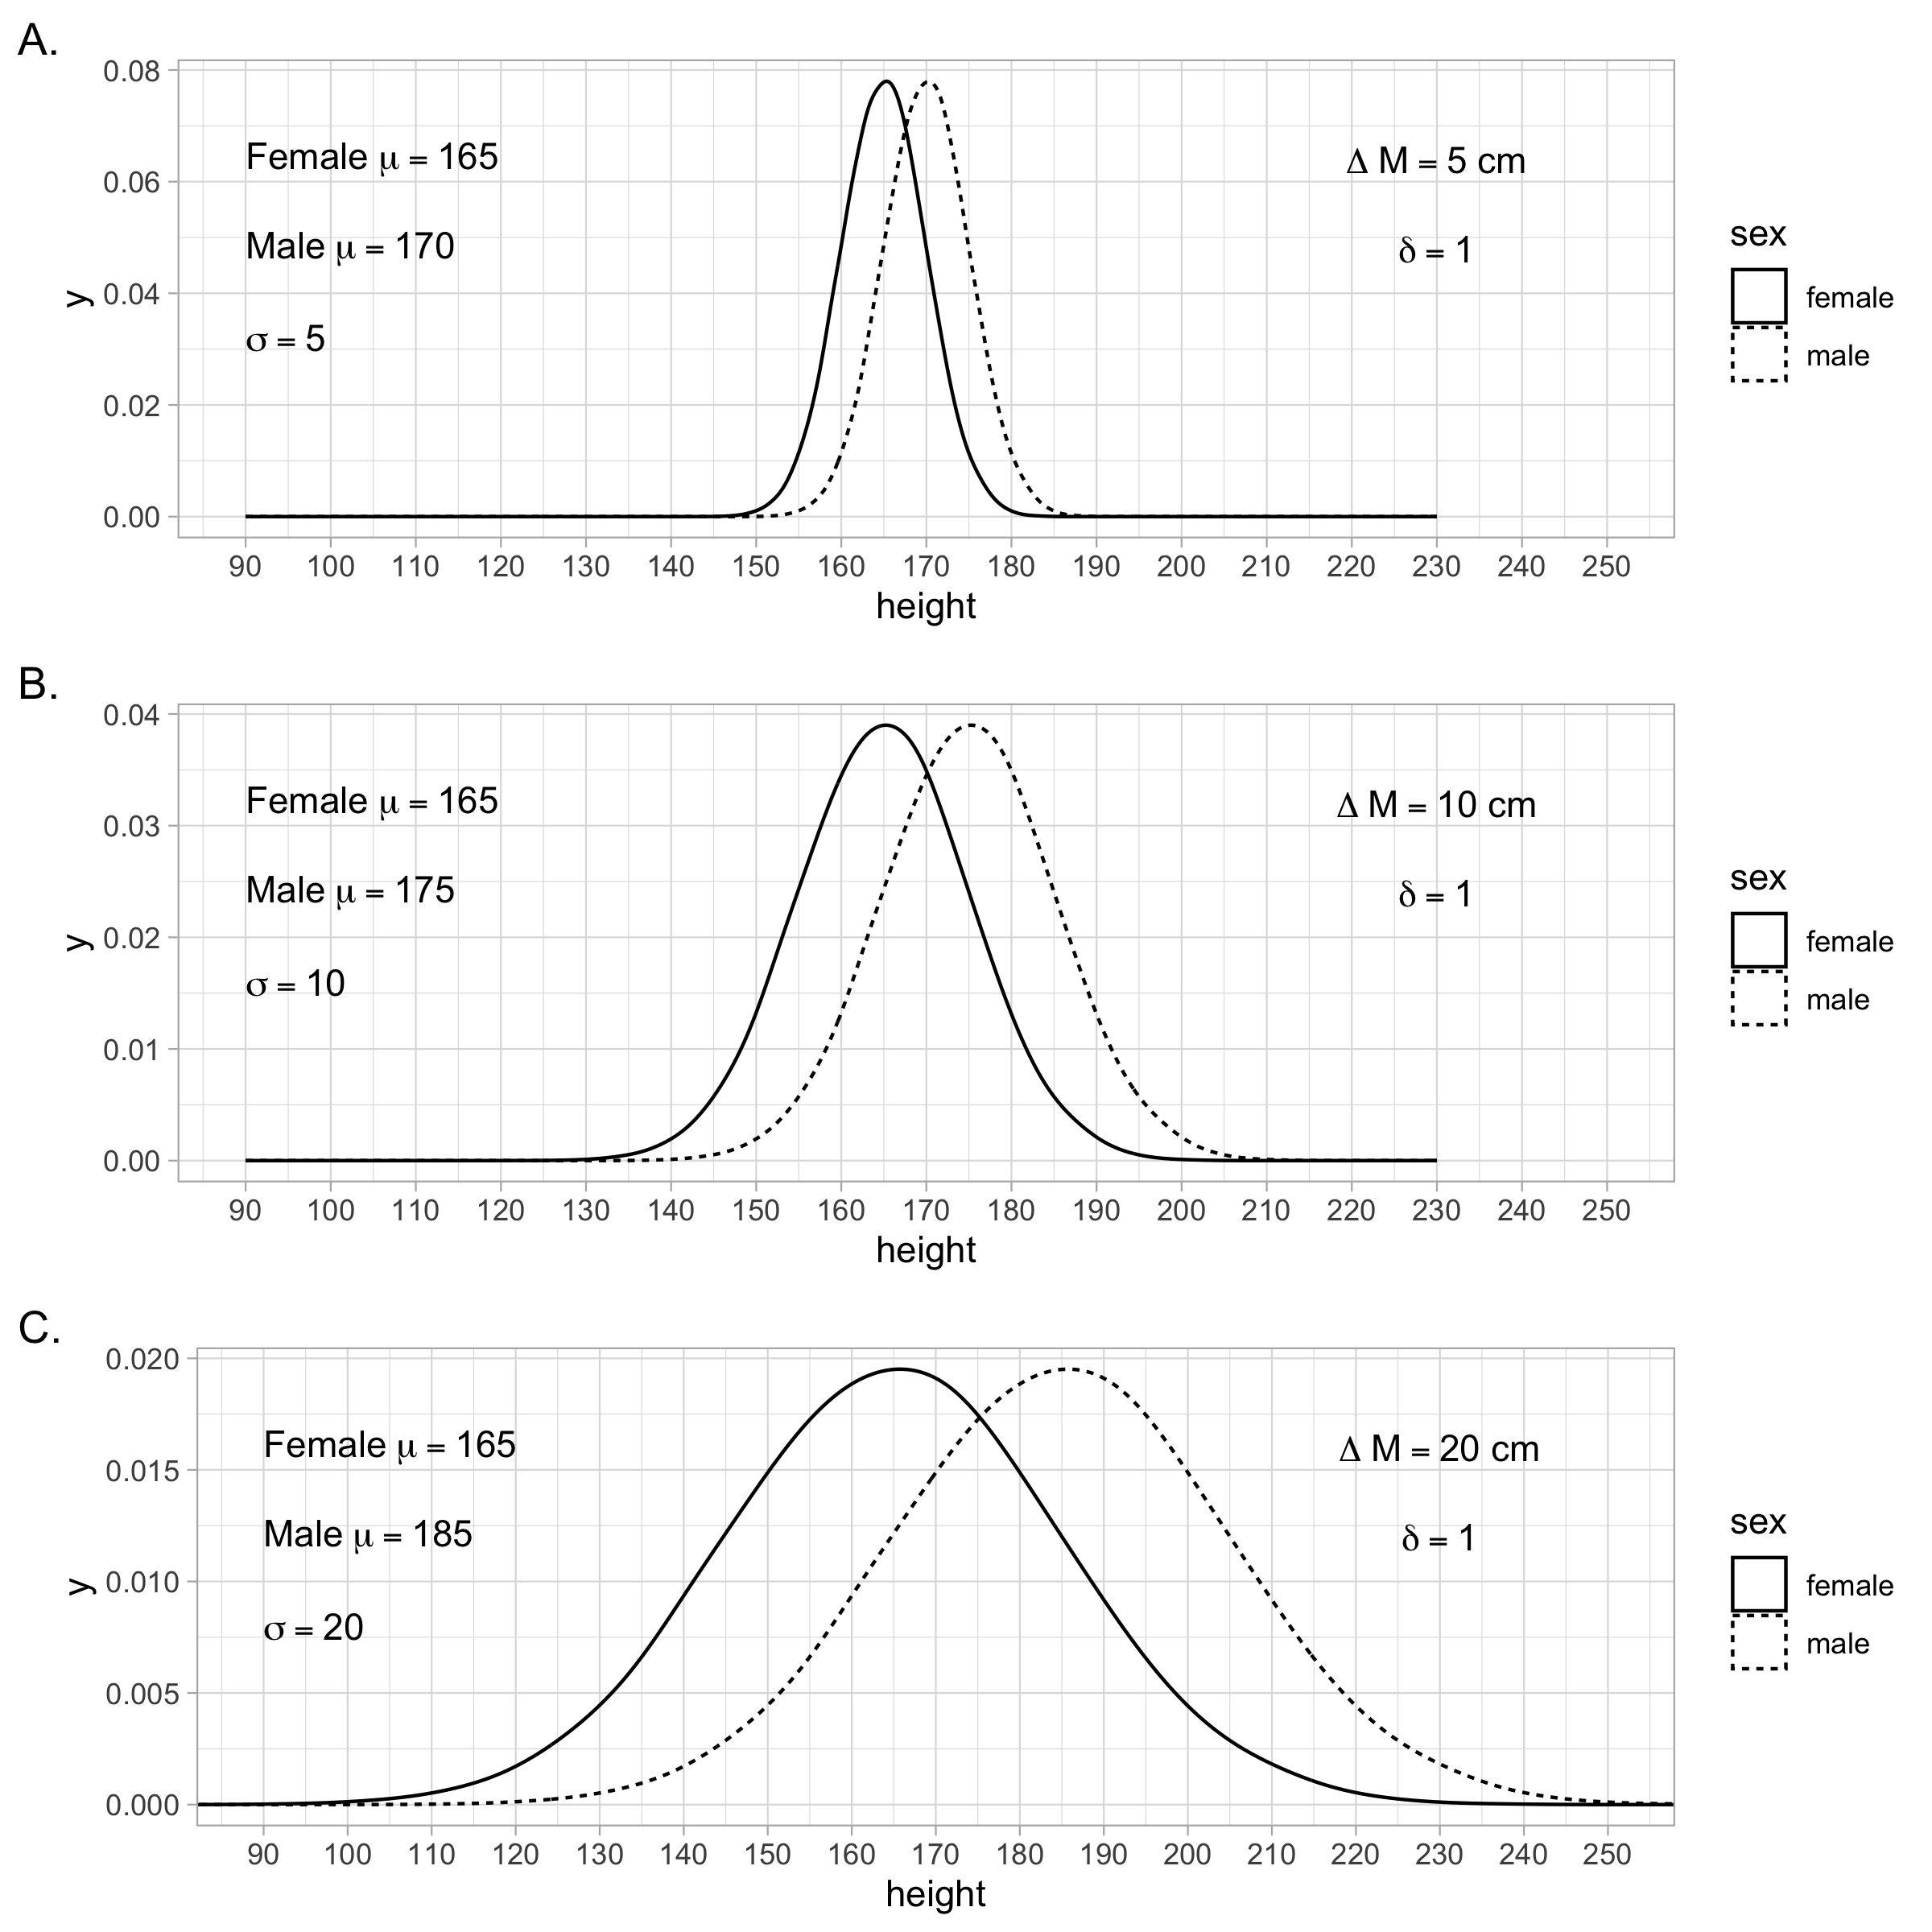
\includegraphics[width=1\linewidth]{ch_populations/images/dvalue_ex3} \caption[Caveats for standardized mean difference]{The three scenarios in this figure illustrate that a Standardized Mean Difference (i.e., population $d$-value or $\delta$) can remain constant across scenarios when there is a change in the raw difference (i.e., $\Delta M$) between the population means. This SMD is consistent across the three scenario despite a change in the mean difference using original units; this occurs because the standard deviations also changes across the three scenarios.}\label{fig:dex3}
\end{figure}

\hypertarget{comparisons-different-sigma}{%
\section{\texorpdfstring{Comparisons: Different \(\sigma\)}{Comparisons: Different \textbackslash sigma}}\label{comparisons-different-sigma}}

The calculation of the standardized mean difference values (\(\delta\)-values) above assumed that the two populations had identical standard deviations. In some scenarios, you might reasonably expect the standard deviations to be different for two populations. When the \textbf{populations} being compared have different standard deviations, we can still calculate a standardized mean difference (i.e, \(\delta\)-value) but we need to pick one of the standard deviations to use in the formula. In many cases, it makes sense to think of one population as the frame of reference for the comparison; a ``Control'' population of sorts. In this case, you use the standard deviation of the control population as the reference/denominator when calculating the \(\delta\)-value as illustrated in Formula \eqref{eq:popsmdcontrolch4} below. Make sure you recognize we are talking about a scenario with different population standard deviations (not sample standard deviations) as the appropriate situation for this type of calculation.

\begin{equation} 
\delta =  \frac{\mu_{1} - \mu_{2}}{\sigma_{control}}
      \label{eq:popsmdcontrolch4}
\end{equation}

\hypertarget{comparisons-repeated-measures}{%
\section{Comparisons: Repeated Measures}\label{comparisons-repeated-measures}}

Sometimes we measures the members of a single population twice and are interested in the change across occasions. Consider a scenario where everyone in a large population (\emph{N} = 1000000) attempts to loose weight over a given period of time. We weigh everyone in the population at time 1 before the weight loss attempt. Then we weigh everyone in the population at time 2 after the weight loss attempt.

Think of this scenario concretely with respect to how we would record this information. Imagine a large spreadsheet with 1000000 rows - each representing a person. There are two columns. The first column contains time 1 weights. The second column contains time 2 weights. We are interested in how weights changed across the times. So we create a third column, called diff, by subtracting time 1 weight from time 2 weights. That is, diff = time 2 weight - time 1 weight. The new diff column indicates how the weights for each person have changed over the diet. We can think of this single column of differences as being a population. This column is used to calculate the repeated-measures \(\delta\)-value. Specifically, the mean of the diff column (\(bar{x}_{diff}\)) and the standard deviation of the diff column (\(s_{diff}\)) are used in Formula \eqref{eq:popsmddiffch4} below:

\begin{equation} 
\delta =  \frac{\mu_{diff}}{\sigma_{diff}}
      \label{eq:popsmddiffch4}
\end{equation}

\hypertarget{comparison-benchmarks}{%
\section{Comparison Benchmarks}\label{comparison-benchmarks}}

Regardless of how the standardized mean difference (i.e., \(\delta\)-value) is calculated, Cohen suggested that the values of 0.20, 0.50, and 0.80 correspond to the effect size labels of small, medium, and large, respectively \citep{cohen1988}. These effect sizes are illustrated in Figure \ref{fig:dex4}. As described in an interesting \href{https://replicationindex.com/2015/09/22/the-statistical-power-of-abnormal-social-psychological-research-a-revew-by-jacob-cohen/}{blog post}, these benchmark values came from reviewing a single issue of the \emph{Journal of Abnormal and Social Psychology}. Basing benchmarks on such a small number of studies is potentially problematic - as is the fact that the that time all the studies were prone to publication bias. A recent investigation \citep[see][]{schafer2019meaningfulness} of effect sizes in pre-registered studies, with no publication bias, suggests substantially lower benchmark values.

\begin{figure}
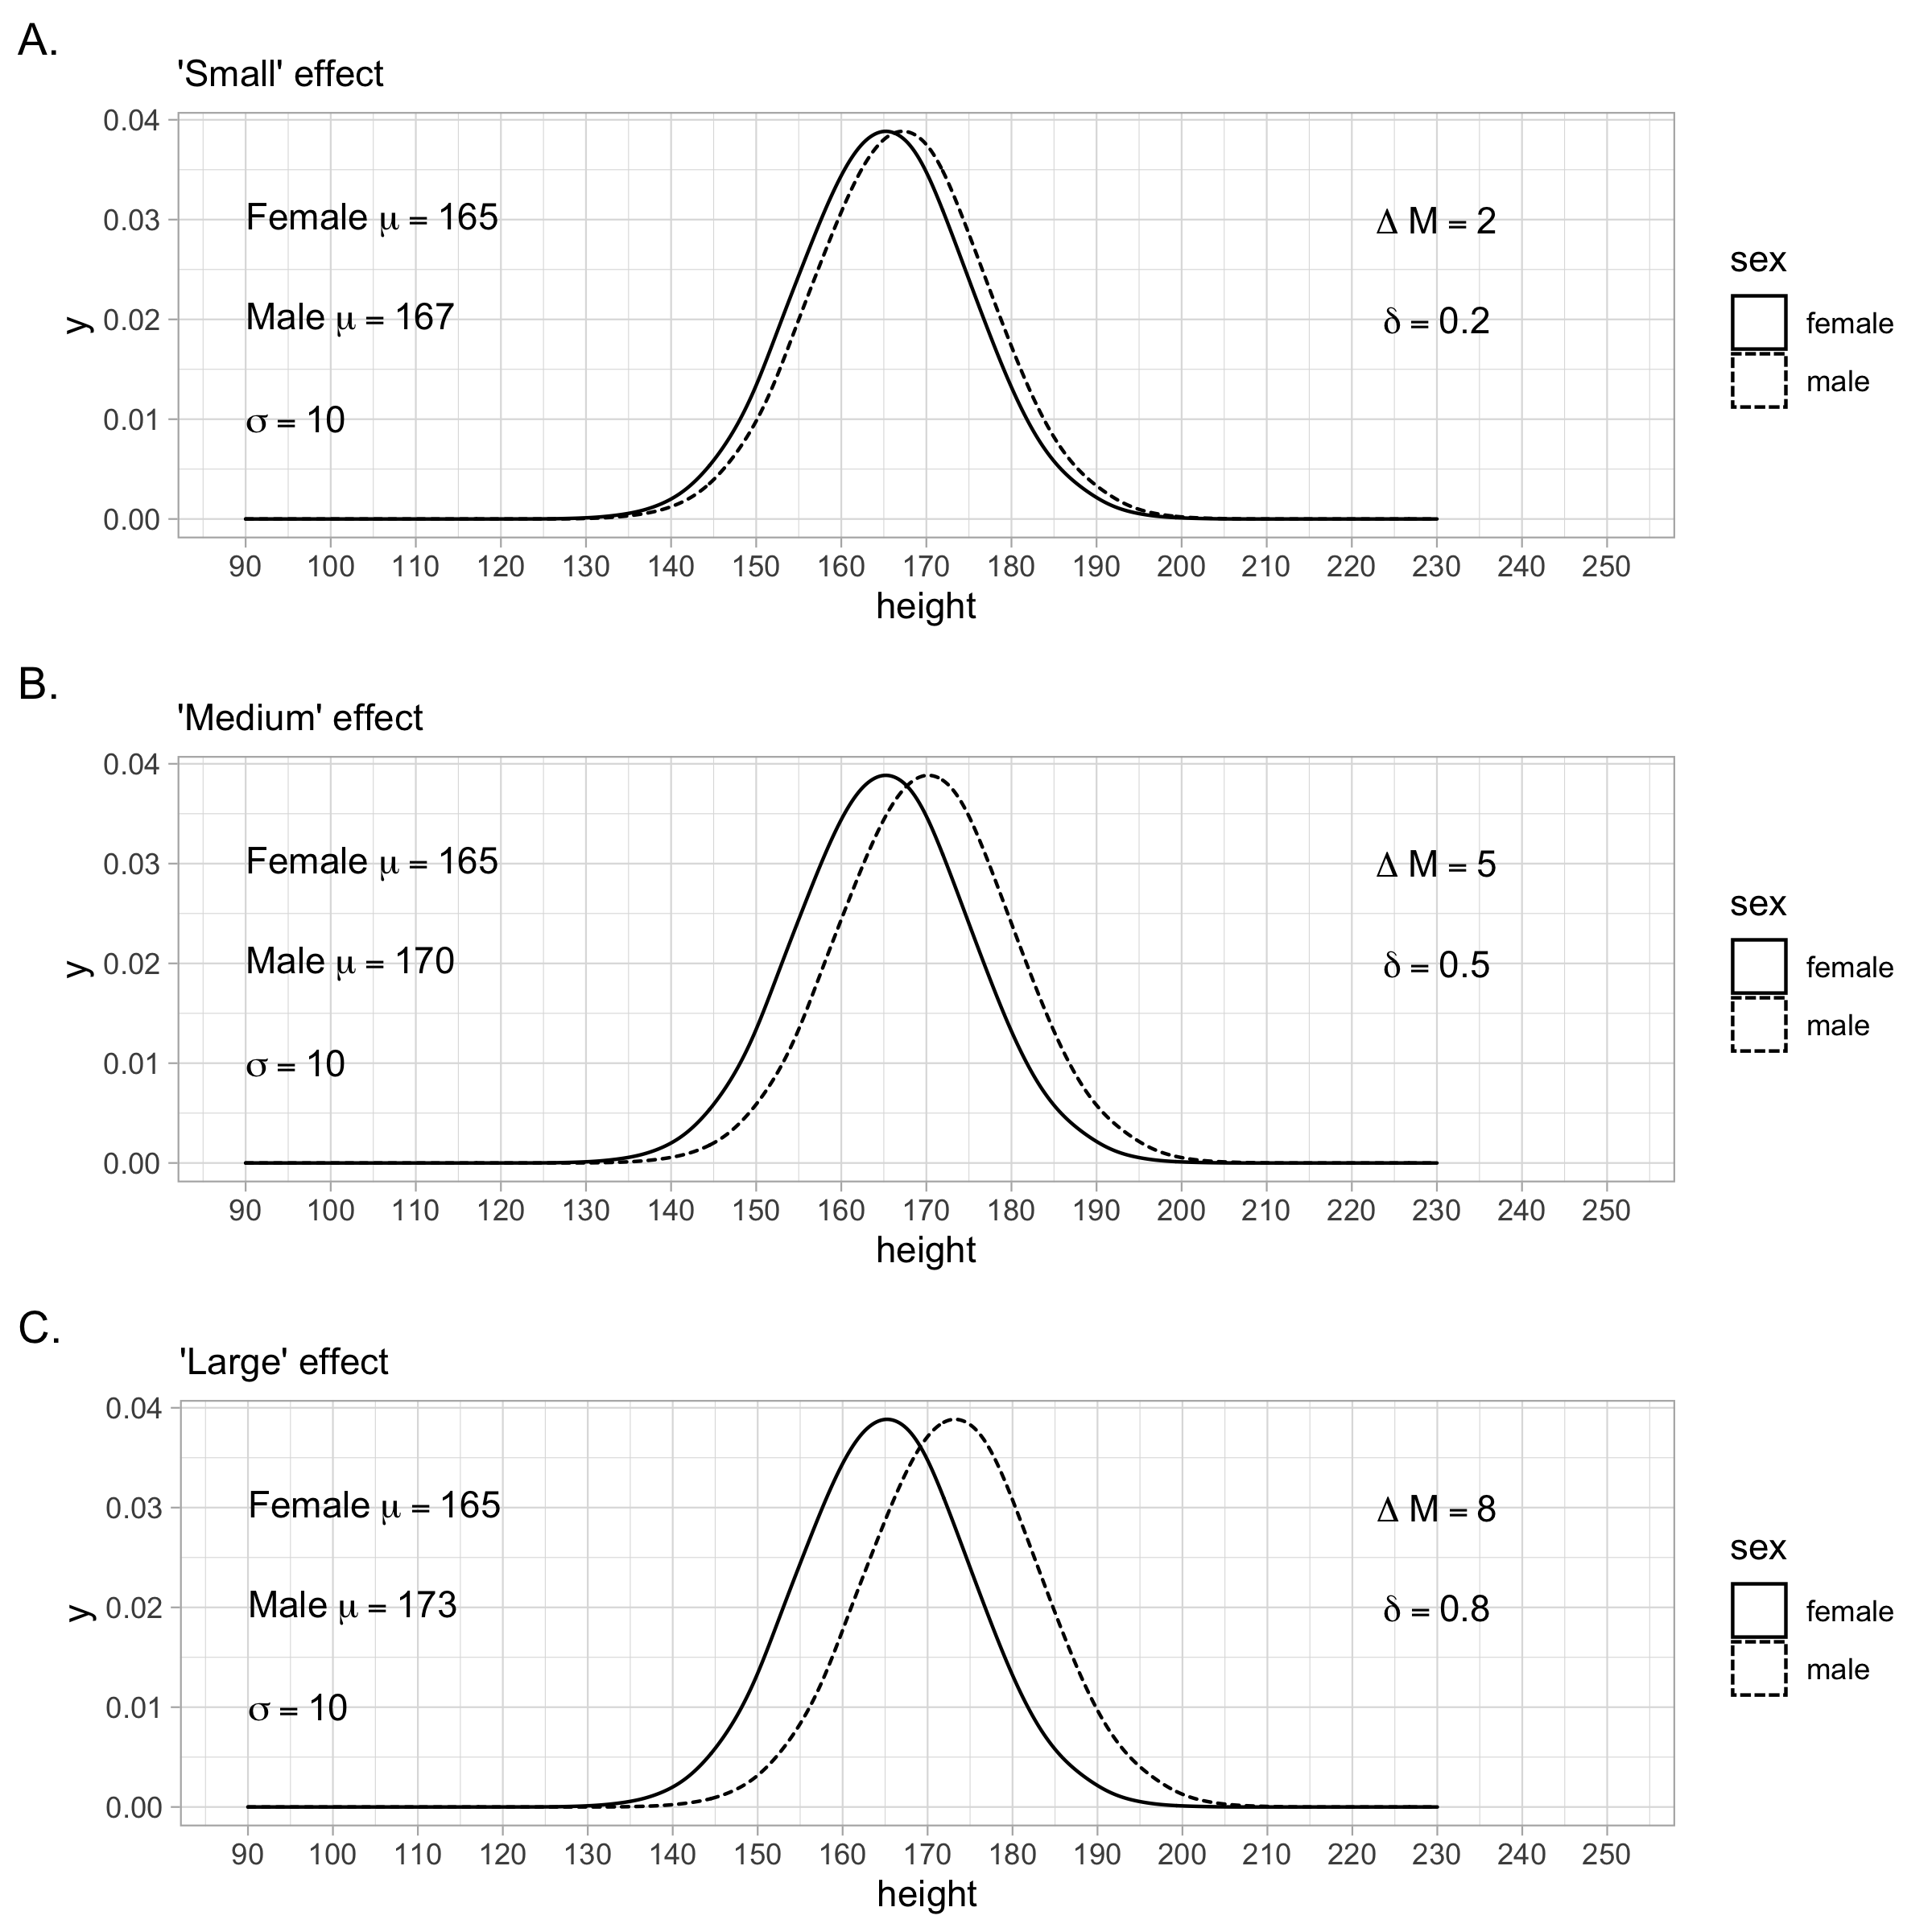
\includegraphics[width=1\linewidth]{ch_populations/images/dvalue_ex4} \caption{Cohen's (1988) effect size benchmarks}\label{fig:dex4}
\end{figure}

You can visualize any \(\delta\) value (i.e., population \(d\)-value) using the rpsychologist \href{https://rpsychologist.com/d3/cohend/}{website}. This website also provides a number of interesting statistics such as the percentage of overlapping values in two populations for a given \(\delta\)/d value. Take a minute to use this website now.

Cohen's benchmarks for standardized mean differences are displayed in the table below. These effect size labels should be interpreted with caution. The magnitude of an effect is best considered in the context of the field of research and the consequences of an effect on individuals in both the short and long run.

\begin{longtable}[]{@{}cc@{}}
\toprule
Cohen (1988) Label & Value\tabularnewline
\midrule
\endhead
Small & \(\delta\) = .20\tabularnewline
Medium & \(\delta\) = .50\tabularnewline
Large & \(\delta\) = .80\tabularnewline
\bottomrule
\end{longtable}

\hypertarget{population-relations}{%
\section{Population relations}\label{population-relations}}

Often researchers are interested in the extent to which one variable is related to another variable. For example, to what extent does variability in weight relate to variability in height? In other words, is there a relation between weight and height? One approach to this question to calculate a regression equation relating weight to height - this provides an index of the relation in the original units of the variables. Here we focus on a second approach to describing the relation between variable, namely, the correlation. The correlation is standardized effect size for the \emph{linear} relation between two variables.

A population correlation is represented by the symbol \(\rho\) (pronounced rho) and calculated using Formula \eqref{eq:poprho4} below. The correlation may range from -1.00 to 1.00. A strong negative correlation indicates that as one variable increases the other decreases. A positive correlation indicates that as one variable increases the other increases. There are at least thirteen ways to conceptualize a correlations \citep[see][]{lee1988thirteen} but it's easiest to think of it as an index of the extent to which the variables covary in a linear way.

\begin{equation} 
\rho =  \frac{\Sigma (X - \mu_X)(Y - \mu_Y)}{\sqrt{\Sigma (X - \mu_X)^2\Sigma (Y - \mu_Y)^2}}
      \label{eq:poprho4}
\end{equation}

Because a correlation only provides an index of a linear relation - it is important to plot the data. Weak correlations (close to zero) may indicate there is not a linear relation. But there may still be a relation between the variables - just not one that follows a straight line. Indeed, the same correlation may take many different forms. Consider the data sets from the datasauRus package presented in Figure \ref{fig:datarex}. The graphs for each data set appear quite different. Yet, the following is true for all 12 data sets:

\begin{itemize}
\tightlist
\item
  The mean of X is 54.3 and the standard deviation is 16.8
\item
  The mean of Y is 47.8 and the standard deviation is 26.9
\item
  The correlation between X and Y is \(\rho\) = -.06
\end{itemize}

Therefore, make sure you ALWAYS graph your data. The numbers only tell part of the story.

\begin{figure}
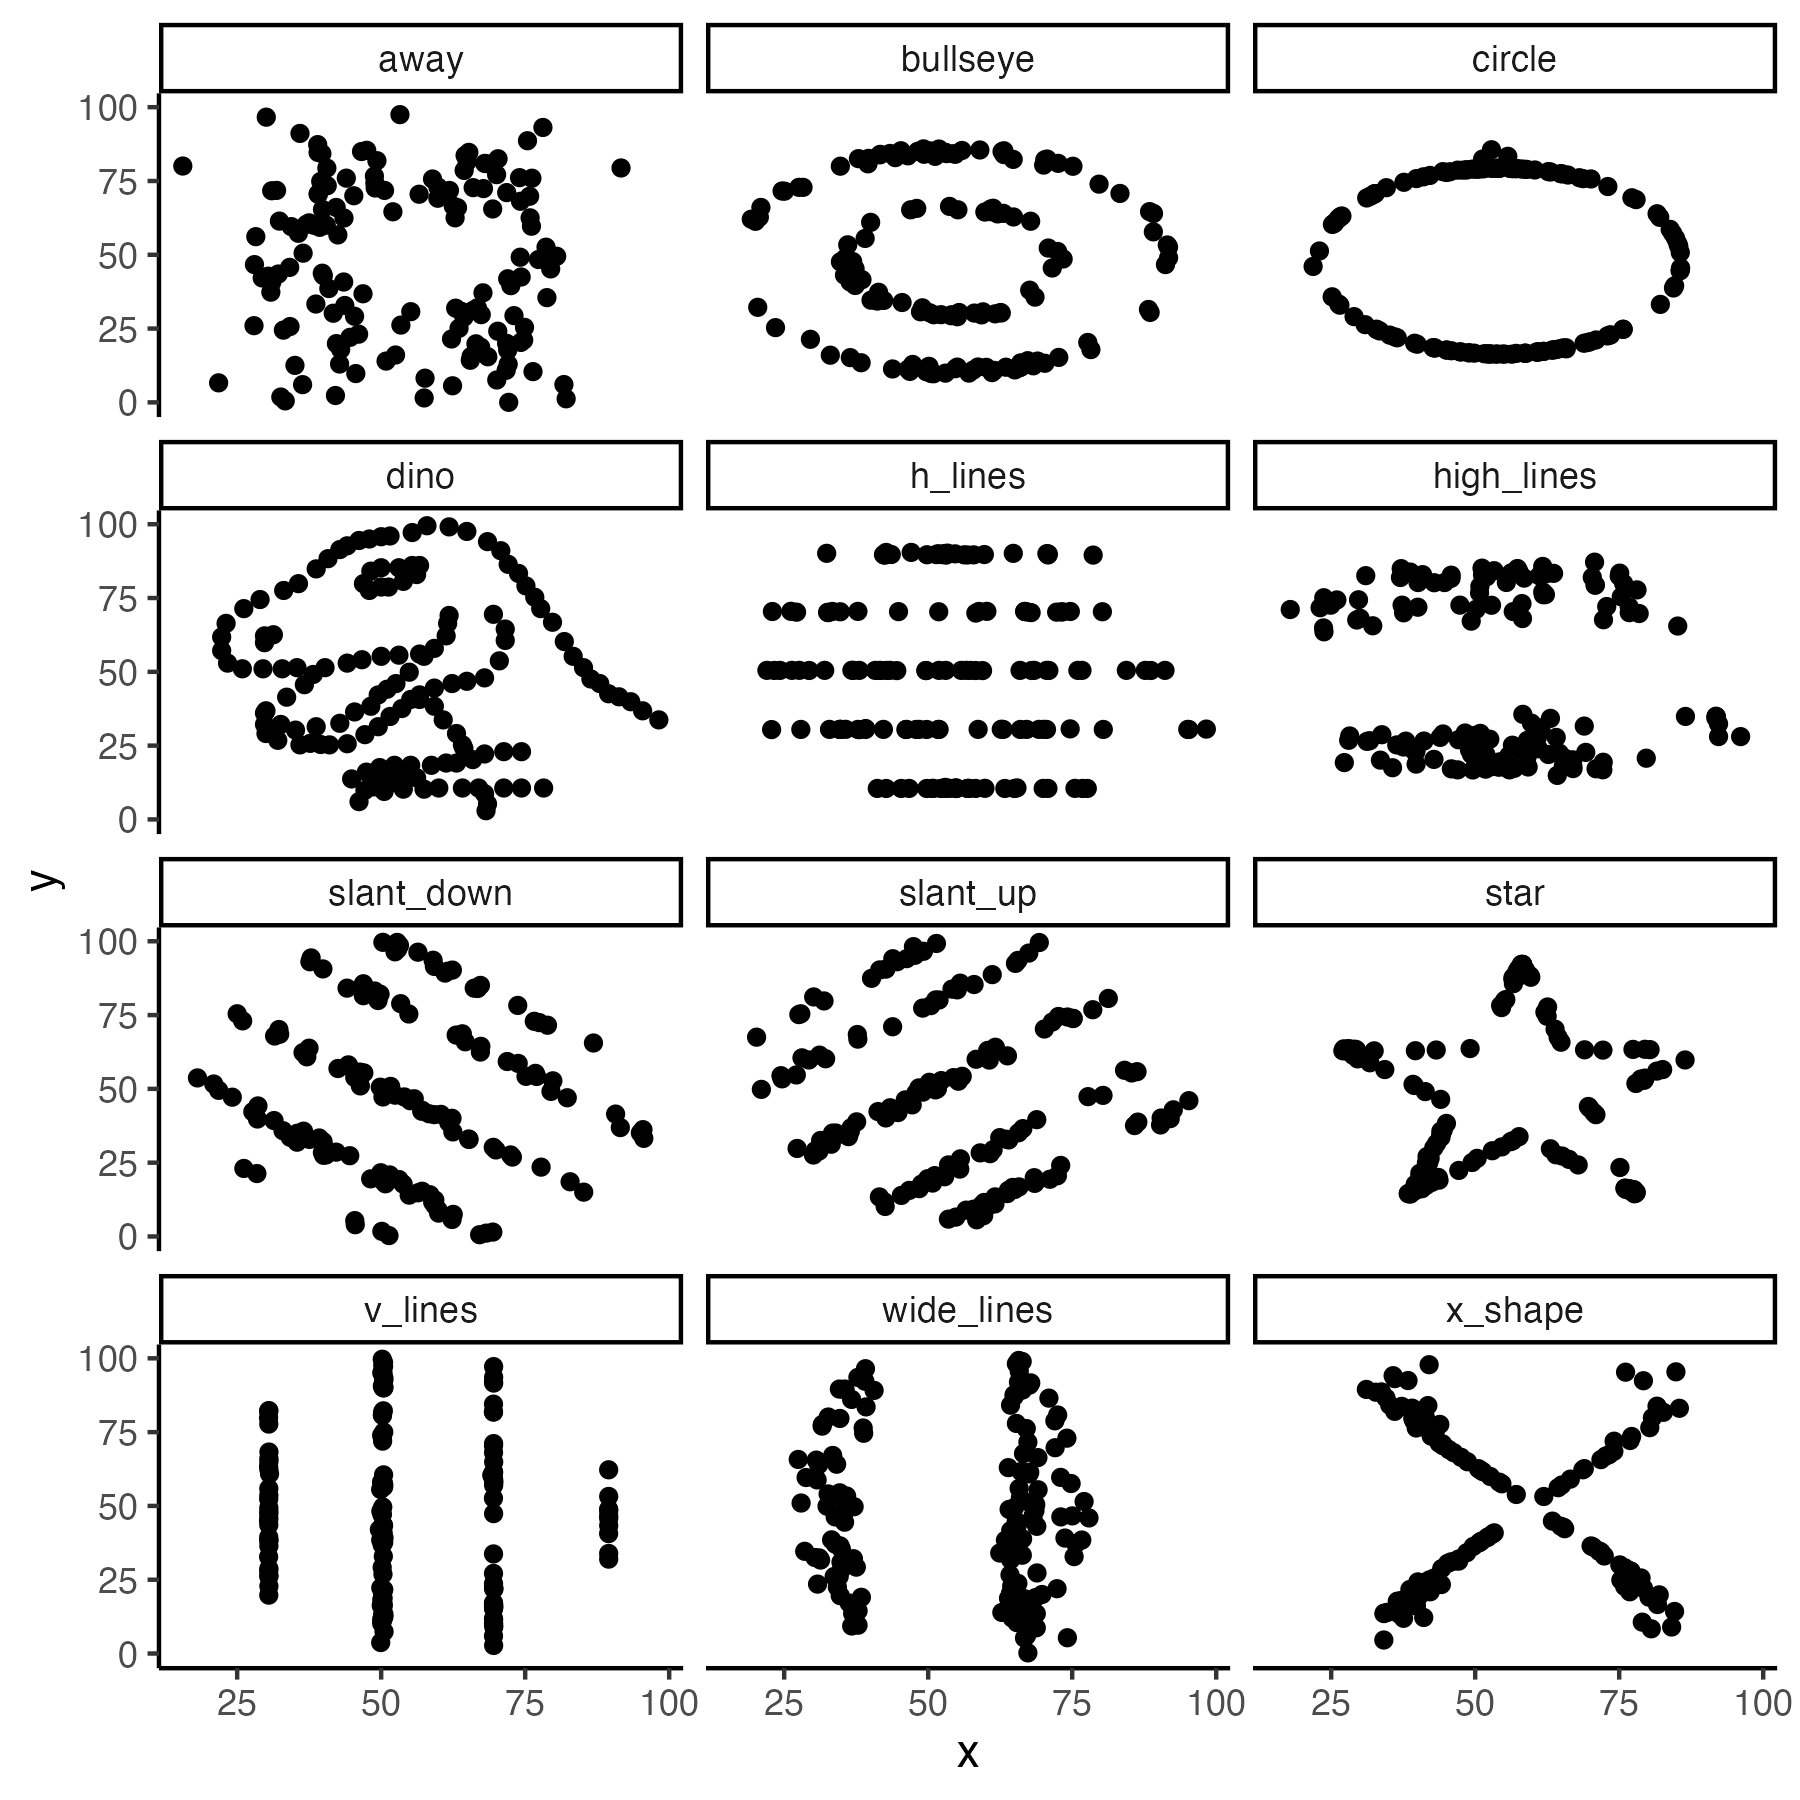
\includegraphics[width=0.8\linewidth,height=0.8\textheight]{ch_populations/images/datarex} \caption{Various data sets with the same correlation, same means, and same standard deviations}\label{fig:datarex}
\end{figure}

\hypertarget{relation-benchmarks}{%
\section{Relation benchmarks}\label{relation-benchmarks}}

Plots of linear relations are presented in Figure \ref{fig:rhoplot}. The three graphs in this figure corresponds to Cohen's benchmarks for correlations (i.e., \(\rho\)), displayed in the table below.

\begin{longtable}[]{@{}cc@{}}
\toprule
Cohen (1988) Label & Value\tabularnewline
\midrule
\endhead
Small & \(\rho\) = .10\tabularnewline
Medium & \(\rho\) = .30\tabularnewline
Large & \(\rho\) = .50\tabularnewline
\bottomrule
\end{longtable}

These effect size labels should be interpreted with caution. The magnitude of an effect is best considered in the context of the field of research and the consequences of an effect on individuals in both the short and long run.

\begin{figure}
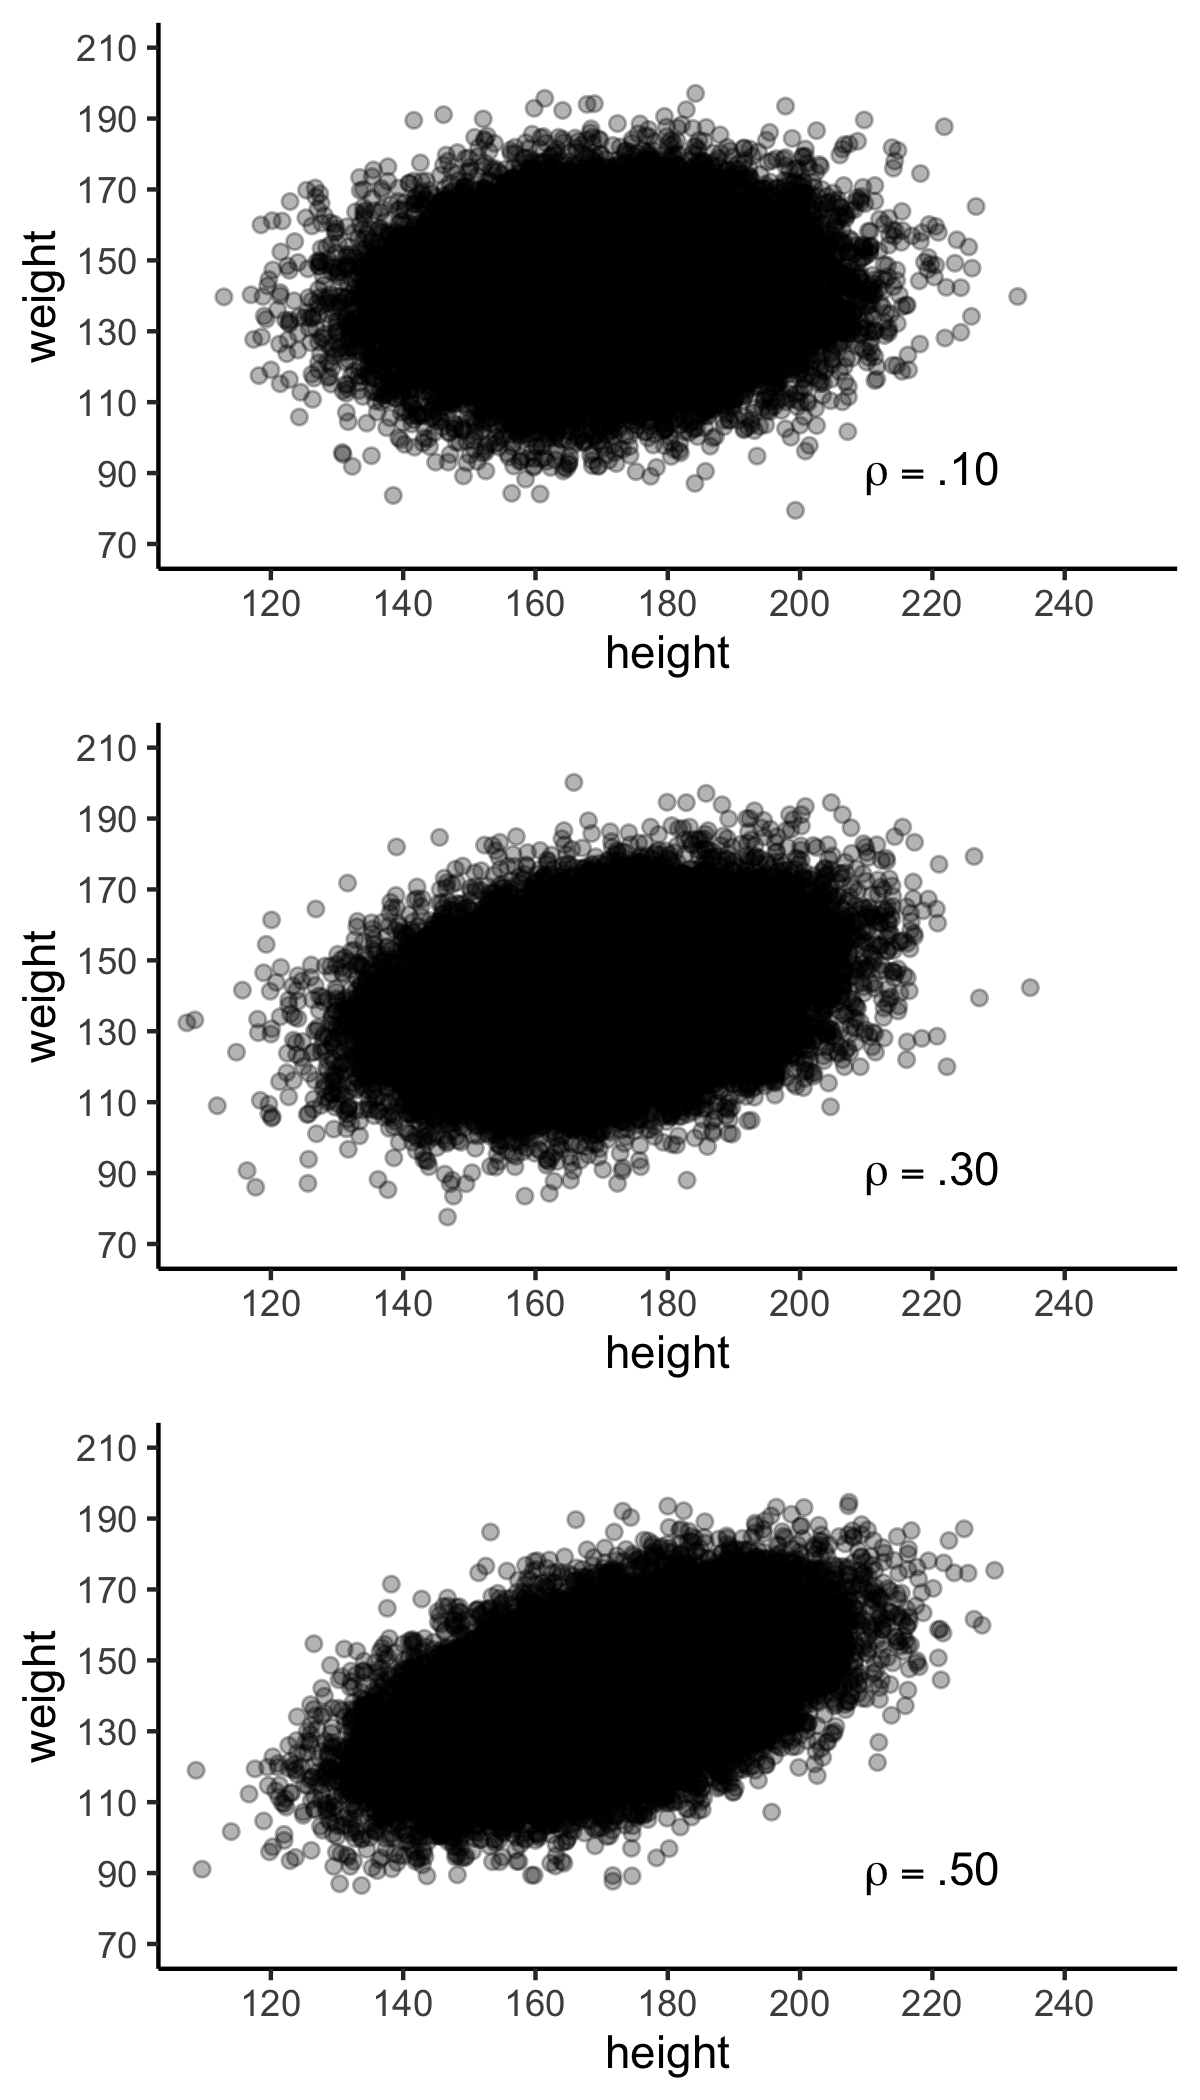
\includegraphics[width=16.67in,height=0.6\textheight]{ch_populations/images/rho_example} \caption{Populations of various strengths.}\label{fig:rhoplot}
\end{figure}

\newpage

\hypertarget{key-points}{%
\section{Key points}\label{key-points}}

\begin{enumerate}
\def\labelenumi{\arabic{enumi}.}
\item
  Populations are described using numbers called parameters.
\item
  Population-level parameters are often represented using Greek letter.
\item
  Commonly used parameters include mean (\(\mu\) or \(\bar{X}\)), variance (\(\sigma^2\)), or standard deviation (\(\sigma\)).
\item
  Individual scores can be expressed in standardized units.
\item
  Population differences can be described in original raw units or standardized units called the standardized mean difference (SMD).
\item
  SMD is based on the premise that the two population being compared have the same standard deviation.
\item
  SMD is a ratio that compares two numbers (the numerator and the denominator).
\item
  Make sure you understand what is represented by both the numerator and denominator in the SMD ratio.
\item
  SMD (i.e., Cohen's d) represents the number of standard deviations between two population means. Recall both populations have the same standard deviation.
\item
  SMD is indicated at the population level using the Greek letter delta (\(\delta\)). At the sample level we tend to use the term ``\(d\)-value'' or ``Cohen's \(d\)''.
\end{enumerate}

\hypertarget{minor-points}{%
\section{Minor Points}\label{minor-points}}

\begin{enumerate}
\def\labelenumi{\arabic{enumi}.}
\item
  Standardized mean differences are reported with a leading zero: \(delta\) = 0.50.
\item
  Correlations are reported \emph{without} a leading zero: \(rho\) = .30.
\item
  The difference in reporting is an APA-style issue. Values that are bounded between 0 and 1 (or between -1 and +1) are reported without a leading zero. Values that are not bounded (such as \(\delta\) values) are reported with the leading zero.
\end{enumerate}

\hypertarget{self-assessment}{%
\section{Self Assessment}\label{self-assessment}}

\begin{enumerate}
\def\labelenumi{\arabic{enumi}.}
\item
  What is the difference between parameters and statistics?
\item
  Are the formulas (excluding notation differences) always the same for parameters and statistics? If not, explain why not?
\item
  Grade 4 students in Ontario are taller than the Grade 3 students. Specifically, \(\delta\) = 0.30. How would you describe what this value means to an audience of experts at a conference? How would you describe what this values means to community members during a talk at the local public library?
\item
  We reviewed three different ways of calculating a standardized mean different (\(\delta\)). What is the appropriate circumstance to use each formula? Describe a concrete scenario for each one.
\item
  There is a strong relation between two variables that follows and upside-down U-shape. Would you expect there to be a strong correlation between these two variables? Why or why not?
\end{enumerate}

\hypertarget{graphing}{%
\chapter{Graphing}\label{graphing}}

\hypertarget{required}{%
\section{Required}\label{required}}

The data files below are used in this chapter. The files are available at: \url{https://github.com/dstanley4/psyc6060bookdown}

\begin{longtable}[]{@{}l@{}}
\toprule
Required Data\tabularnewline
\midrule
\endhead
data\_movies.csv\tabularnewline
\bottomrule
\end{longtable}

The following packages CRAN must be installed:

\begin{longtable}[]{@{}l@{}}
\toprule
Required CRAN Packages\tabularnewline
\midrule
\endhead
tidyverse\tabularnewline
RColorBrewer\tabularnewline
remotes\tabularnewline
\bottomrule
\end{longtable}

The following GitHub packages must be installed:

\begin{longtable}[]{@{}l@{}}
\toprule
Required GitHub Packages\tabularnewline
\midrule
\endhead
dill/emoGG\tabularnewline
\bottomrule
\end{longtable}

After the remotes package is installed, it can be used to install a package from GitHub:

\begin{Shaded}
\begin{Highlighting}[]
\NormalTok{remotes}\OperatorTok{::}\KeywordTok{install_github}\NormalTok{(}\StringTok{"dill/emoGG"}\NormalTok{)}
\end{Highlighting}
\end{Shaded}

\hypertarget{data}{%
\section{Data}\label{data}}

To learn about making graphs using the tidyverse we use movie ratings and box office data obtained at the time of writing. Movie ratings were obtained from the \href{https://www.imdb.com}{IMDB} and \href{https://www.rottentomatoes.com}{RottenTomatoes}. Box office data (in millions of dollars) was obtained from \href{https://www.boxofficemojo.com}{Box Office Mojo}. If you enjoy learning about movies these are all excellent sites.

We begin by loading data\_movies.csv using read\_csv(), not read.csv():

\begin{Shaded}
\begin{Highlighting}[]
\NormalTok{movie_data <-}\StringTok{ }\KeywordTok{read_csv}\NormalTok{(}\StringTok{"data_movies.csv"}\NormalTok{)}
\end{Highlighting}
\end{Shaded}

Next we inspect movie\_data using the print() command. We see that each row of the data set corresponds to a superhero movie.

\begin{Shaded}
\begin{Highlighting}[]
\KeywordTok{print}\NormalTok{(movie_data)}
\end{Highlighting}
\end{Shaded}

\begin{verbatim}
## # A tibble: 8 x 7
##   title short_title  year  imdb tomatoes_aud boxoffice
##   <chr> <chr>       <dbl> <dbl>        <dbl>     <dbl>
## 1 Iron~ Iron         2008   7.9           96       585
## 2 Thor~ Thor         2017   7.9           93       854
## 3 Aven~ AV3          2018   8.5           91      2048
## 4 Aven~ AV4          2019   8.7           91      2744
## 5 Man ~ Sup          2013   7.1           75       668
## 6 Batm~ BvS          2015   6.5           63       873
## 7 Just~ JL           2017   6.5           72       657
## 8 Wond~ WW           2017   7.5           88       821
## # ... with 1 more variable: studio <chr>
\end{verbatim}

Next we use glimpse() to see the columns.

\begin{Shaded}
\begin{Highlighting}[]
\KeywordTok{glimpse}\NormalTok{(movie_data)}
\end{Highlighting}
\end{Shaded}

\begin{verbatim}
## Rows: 8
## Columns: 7
## $ title        <chr> "Iron Man", "Thor Ragnarok", "Aven...
## $ short_title  <chr> "Iron", "Thor", "AV3", "AV4", "Sup...
## $ year         <dbl> 2008, 2017, 2018, 2019, 2013, 2015...
## $ imdb         <dbl> 7.9, 7.9, 8.5, 8.7, 7.1, 6.5, 6.5,...
## $ tomatoes_aud <dbl> 96, 93, 91, 91, 75, 63, 72, 88
## $ boxoffice    <dbl> 585, 854, 2048, 2744, 668, 873, 65...
## $ studio       <chr> "Marvel", "Marvel", "Marvel", "Mar...
\end{verbatim}

The title and short\_title columns provide the full title and short title for each movie. Additionally, the IMDB rating, the Rotten Tomatoes Audience rating, and the Box Office Mojo revenue numbers are provided in the imdb, tomatoes\_aud, and boxoffice columns, respectively. Finally, the last column, studio, indicates the studio that made the movie (Marvel or DC).

It is extremely important for graphing and analyses that you tell R which columns are composed of categorical variables. We do that using the as\_factor command. The as\_factor command turns a column into a categorical column. We use the mutate command to replace the original column with the column that has been defined as a categorical variables using as\_factor.

\begin{Shaded}
\begin{Highlighting}[]
\NormalTok{movie_data <-}\StringTok{ }\NormalTok{movie_data }\OperatorTok\StringTok{ }
\StringTok{  }\KeywordTok{mutate}\NormalTok{(}\KeywordTok{across}\NormalTok{(}\DataTypeTok{.cols =} \KeywordTok{where}\NormalTok{(is.character), }
                \DataTypeTok{.fns =}\NormalTok{ as_factor))}
\end{Highlighting}
\end{Shaded}

We can confirm the column type has changed by using the glimpse() command again and examing the column types:

\begin{Shaded}
\begin{Highlighting}[]
\KeywordTok{glimpse}\NormalTok{(movie_data)}
\end{Highlighting}
\end{Shaded}

\begin{verbatim}
## Rows: 8
## Columns: 7
## $ title        <fct> Iron Man, Thor Ragnarok, Avengers ...
## $ short_title  <fct> Iron, Thor, AV3, AV4, Sup, BvS, JL...
## $ year         <dbl> 2008, 2017, 2018, 2019, 2013, 2015...
## $ imdb         <dbl> 7.9, 7.9, 8.5, 8.7, 7.1, 6.5, 6.5,...
## $ tomatoes_aud <dbl> 96, 93, 91, 91, 75, 63, 72, 88
## $ boxoffice    <dbl> 585, 854, 2048, 2744, 668, 873, 65...
## $ studio       <fct> Marvel, Marvel, Marvel, Marvel, DC...
\end{verbatim}

\hypertarget{graph-basics}{%
\section{Graph basics}\label{graph-basics}}

In this section we teach you how to make a graph from first principles to form a foundation for understanding how the tidyverse graphing command ggplot() works. Note, however, that the approach used for creating a graph in this section is for teaching purposes only. Later we will make graphs in a typical, and more efficient, manner.

We start a graph using the ggplot() command. The ggplot() command creates an empty template for the graph. After creating the template we have to add content (like bars) to the graph using the geom\_col() command. We can also add text using the geom\_text() command.

Commands that plot information on the graph, such as geom\_col(), need to know what data set to use to create the graph. We specify the data set to use via the \textbf{data} argument. For example, we use ``data = movie\_data'' to tell a command which data set to use.

Additionally, graphing commands, such as geom\_col(), must know the columns/variables to use within that data set when plotting the graph. Specifically, commands need to know which variable/column will vary over the x- and y-axes. We can indicate these columns via the \textbf{mapping} argument. For example, we use ``mapping = aes(x = short\_title, y = boxoffice)'' to tell ggplot() that we should use the column short\_title along the x-axis and the column boxoffice when determining heights on the y-axis. This information is nested within the aes() command which is short for aesthetic. You are telling ggplot() about the aesthetics for the graph (i.e., which columns to use for the x- and y-axes) using the aes() command. There are a larger number of aesthetics that you can specify within the aes() command (e.g., color, fill, linetype, etc.).

In the examples that follow we tell each command (geom\_col, geom\_text) which data set and columns to use via the \textbf{data} and \textbf{mapping} arguments.

Use geom\_col() to put each boxoffice column value into a bar.

\begin{Shaded}
\begin{Highlighting}[]
\NormalTok{my_graph <-}\StringTok{ }\KeywordTok{ggplot}\NormalTok{() }\OperatorTok{+}
\StringTok{  }\KeywordTok{geom_col}\NormalTok{(}\DataTypeTok{data =}\NormalTok{ movie_data,}
           \DataTypeTok{mapping =} \KeywordTok{aes}\NormalTok{(}\DataTypeTok{x =}\NormalTok{ short_title, }
                         \DataTypeTok{y =}\NormalTok{ boxoffice))}

\KeywordTok{print}\NormalTok{(my_graph)}
\end{Highlighting}
\end{Shaded}

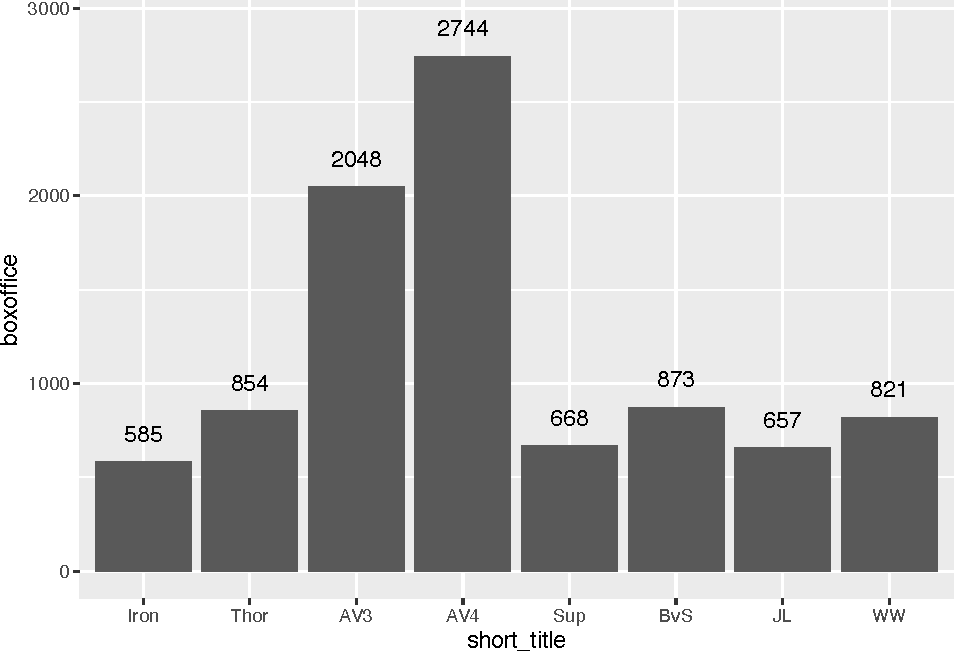
\includegraphics[width=0.65\linewidth]{bookdown_files/figure-latex/unnamed-chunk-108-1}

Next, we want to put the boxoffice revenue above each bar so it easier to interpret. In R terms, we are putting a label above each bar. We want the contents for the labels to come from the boxoffice column. Therefore, we add the geom\_text() command below:

\begin{Shaded}
\begin{Highlighting}[]
\NormalTok{my_graph <-}\StringTok{ }\KeywordTok{ggplot}\NormalTok{() }\OperatorTok{+}
\StringTok{  }\KeywordTok{geom_col}\NormalTok{(}\DataTypeTok{data =}\NormalTok{ movie_data,}
           \DataTypeTok{mapping =} \KeywordTok{aes}\NormalTok{(}\DataTypeTok{x =}\NormalTok{ short_title, }
                         \DataTypeTok{y =}\NormalTok{ boxoffice)) }\OperatorTok{+}
\StringTok{  }\KeywordTok{geom_text}\NormalTok{(}\DataTypeTok{data =}\NormalTok{ movie_data, }
           \DataTypeTok{mapping =} \KeywordTok{aes}\NormalTok{(}\DataTypeTok{x =}\NormalTok{ short_title, }
                         \DataTypeTok{y =}\NormalTok{ boxoffice, }
                         \DataTypeTok{label =}\NormalTok{ boxoffice))}
\KeywordTok{print}\NormalTok{(my_graph)}
\end{Highlighting}
\end{Shaded}

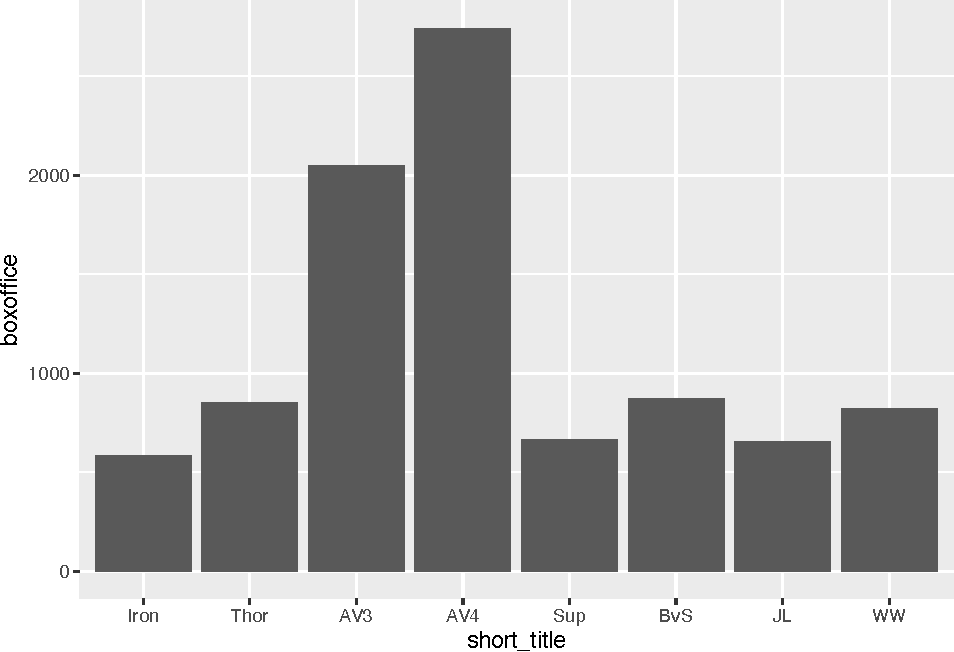
\includegraphics[width=0.65\linewidth]{bookdown_files/figure-latex/unnamed-chunk-109-1}

Unfortunately, when we position the text at the exact height of each column it overlaps with the column making it difficult to read. We fix this on the next page using nudge\_y.

We can nudge each label higher on the y-axis using the \emph{nudge\_y} command. In the above code, we nudge it up 150 units. Since nudge\_y uses the values on the y-axis we are nudging the labels up by 150 million on the y-axis.

\begin{Shaded}
\begin{Highlighting}[]
\NormalTok{my_graph <-}\StringTok{ }\KeywordTok{ggplot}\NormalTok{() }\OperatorTok{+}
\StringTok{  }\KeywordTok{geom_col}\NormalTok{(}\DataTypeTok{data =}\NormalTok{ movie_data,}
           \DataTypeTok{mapping =} \KeywordTok{aes}\NormalTok{(}\DataTypeTok{x =}\NormalTok{ short_title, }
                         \DataTypeTok{y =}\NormalTok{ boxoffice)) }\OperatorTok{+}
\StringTok{  }\KeywordTok{geom_text}\NormalTok{(}\DataTypeTok{data =}\NormalTok{ movie_data, }
           \DataTypeTok{mapping =} \KeywordTok{aes}\NormalTok{(}\DataTypeTok{x =}\NormalTok{ short_title, }
                         \DataTypeTok{y =}\NormalTok{ boxoffice, }
                         \DataTypeTok{label =}\NormalTok{ boxoffice),}
           \DataTypeTok{nudge_y =} \DecValTok{150}\NormalTok{)}

\KeywordTok{print}\NormalTok{(my_graph)}
\end{Highlighting}
\end{Shaded}

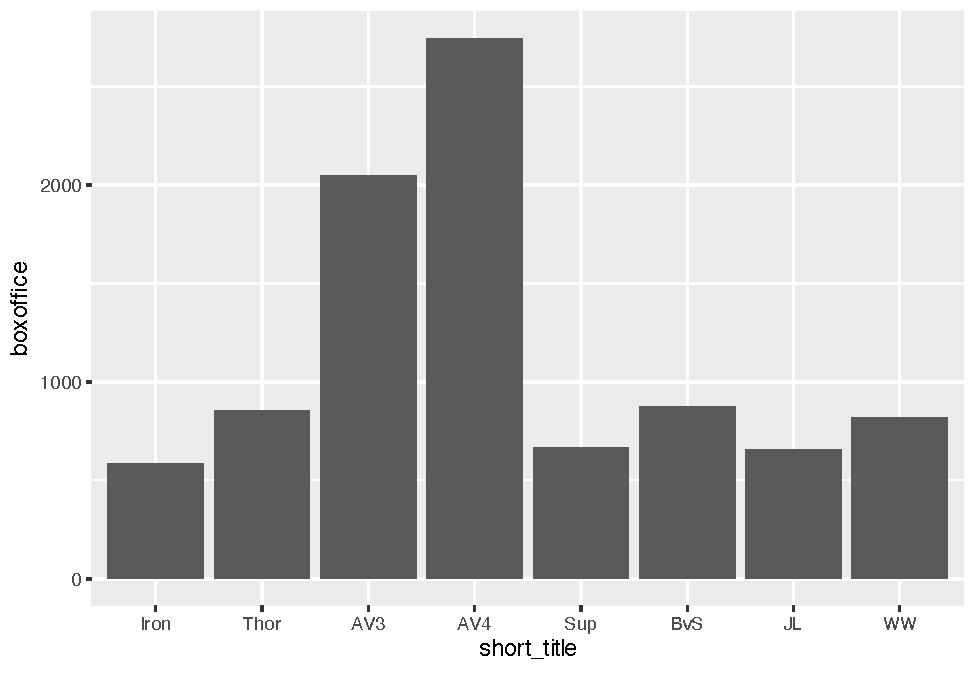
\includegraphics[width=0.65\linewidth]{bookdown_files/figure-latex/unnamed-chunk-110-1}

\hypertarget{graphing-efficiently}{%
\section{Graphing efficiently}\label{graphing-efficiently}}

You may have noticed that creating the graphs the way we did above required repeating the data and mapping assignments within each command (e.g., geom\_text, geom\_col). Fortunately, we can use a shortcut and specify the data and mapping only once in the ggplot() command. Once we do that, the contents of the mapping argument are invisibly copied into each subsequent command (e.g., geom\_col, geom\_text). In this way, we only have to specify the data and the mapping once.

Examine the code below and compare it to the code above. Notice how in the geom\_col() command we don't have anything specified -- the data and mapping from the ggplot command are used. Likewise, notice how in the geom\_text() command we only specify the arguments we need that are different from those in the ggplot command. In this case, that means simply adding the nudge\_y = 150 to the geom\_text command.

\begin{Shaded}
\begin{Highlighting}[]
\NormalTok{my_graph <-}\StringTok{ }\KeywordTok{ggplot}\NormalTok{(}\DataTypeTok{data =}\NormalTok{ movie_data,}
           \DataTypeTok{mapping =} \KeywordTok{aes}\NormalTok{(}\DataTypeTok{x =}\NormalTok{ short_title,}
                         \DataTypeTok{y =}\NormalTok{ boxoffice,}
                         \DataTypeTok{label =}\NormalTok{ boxoffice)) }\OperatorTok{+}
\StringTok{  }\KeywordTok{geom_col}\NormalTok{() }\OperatorTok{+}
\StringTok{  }\KeywordTok{geom_text}\NormalTok{(}\DataTypeTok{nudge_y =} \DecValTok{150}\NormalTok{) }

\KeywordTok{print}\NormalTok{(my_graph)}
\end{Highlighting}
\end{Shaded}

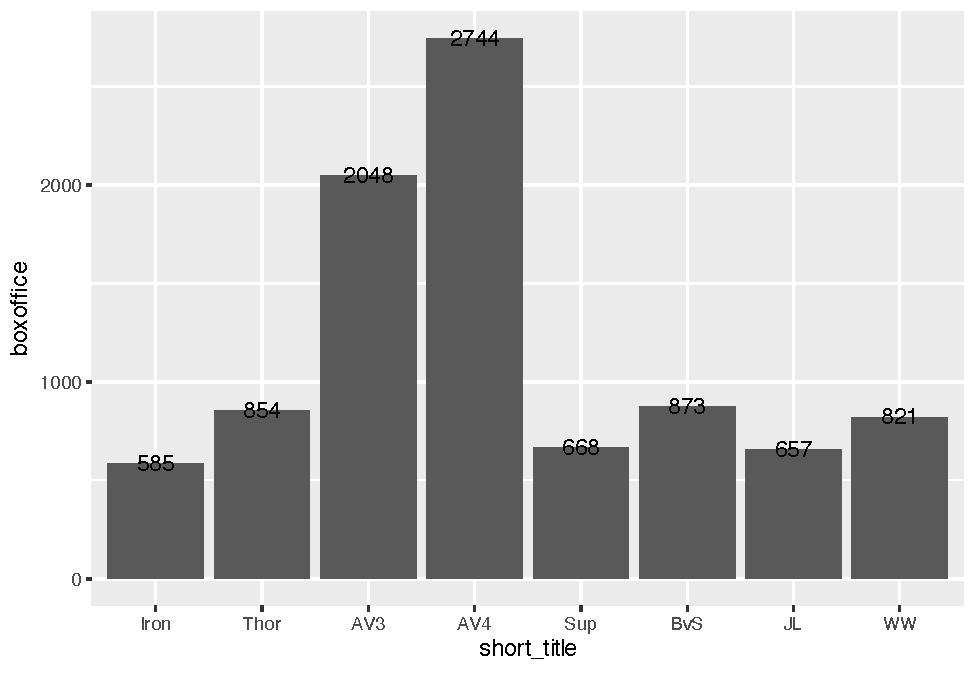
\includegraphics[width=0.65\linewidth]{bookdown_files/figure-latex/unnamed-chunk-111-1}

\hypertarget{aesthetics}{%
\section{Aesthetics}\label{aesthetics}}

Exactly how does that aesthetic, aes(), command work? What happens when we put the data and mapping in the ggplot() command instead of the specific commands such as geom\_col()? When we put data and the mapping arguments in the ggplot() command we set those attributes for the entire graph. To understand this, you need to know that ggplot uses an internal data set that we will call the ``black box'' data set (i.e., inside the \href{https://en.wikipedia.org/wiki/Black_box}{black box} of ggplot). To create a graph ggplot maps/copies columns from your data set (e.g., movie\_data) to an internal data set. This internal data set is then used to create the graph. Figure \ref{fig:showmap} below illustrates what is happening ``inside the black box'' when you create the graph using the code above.

\begin{figure}
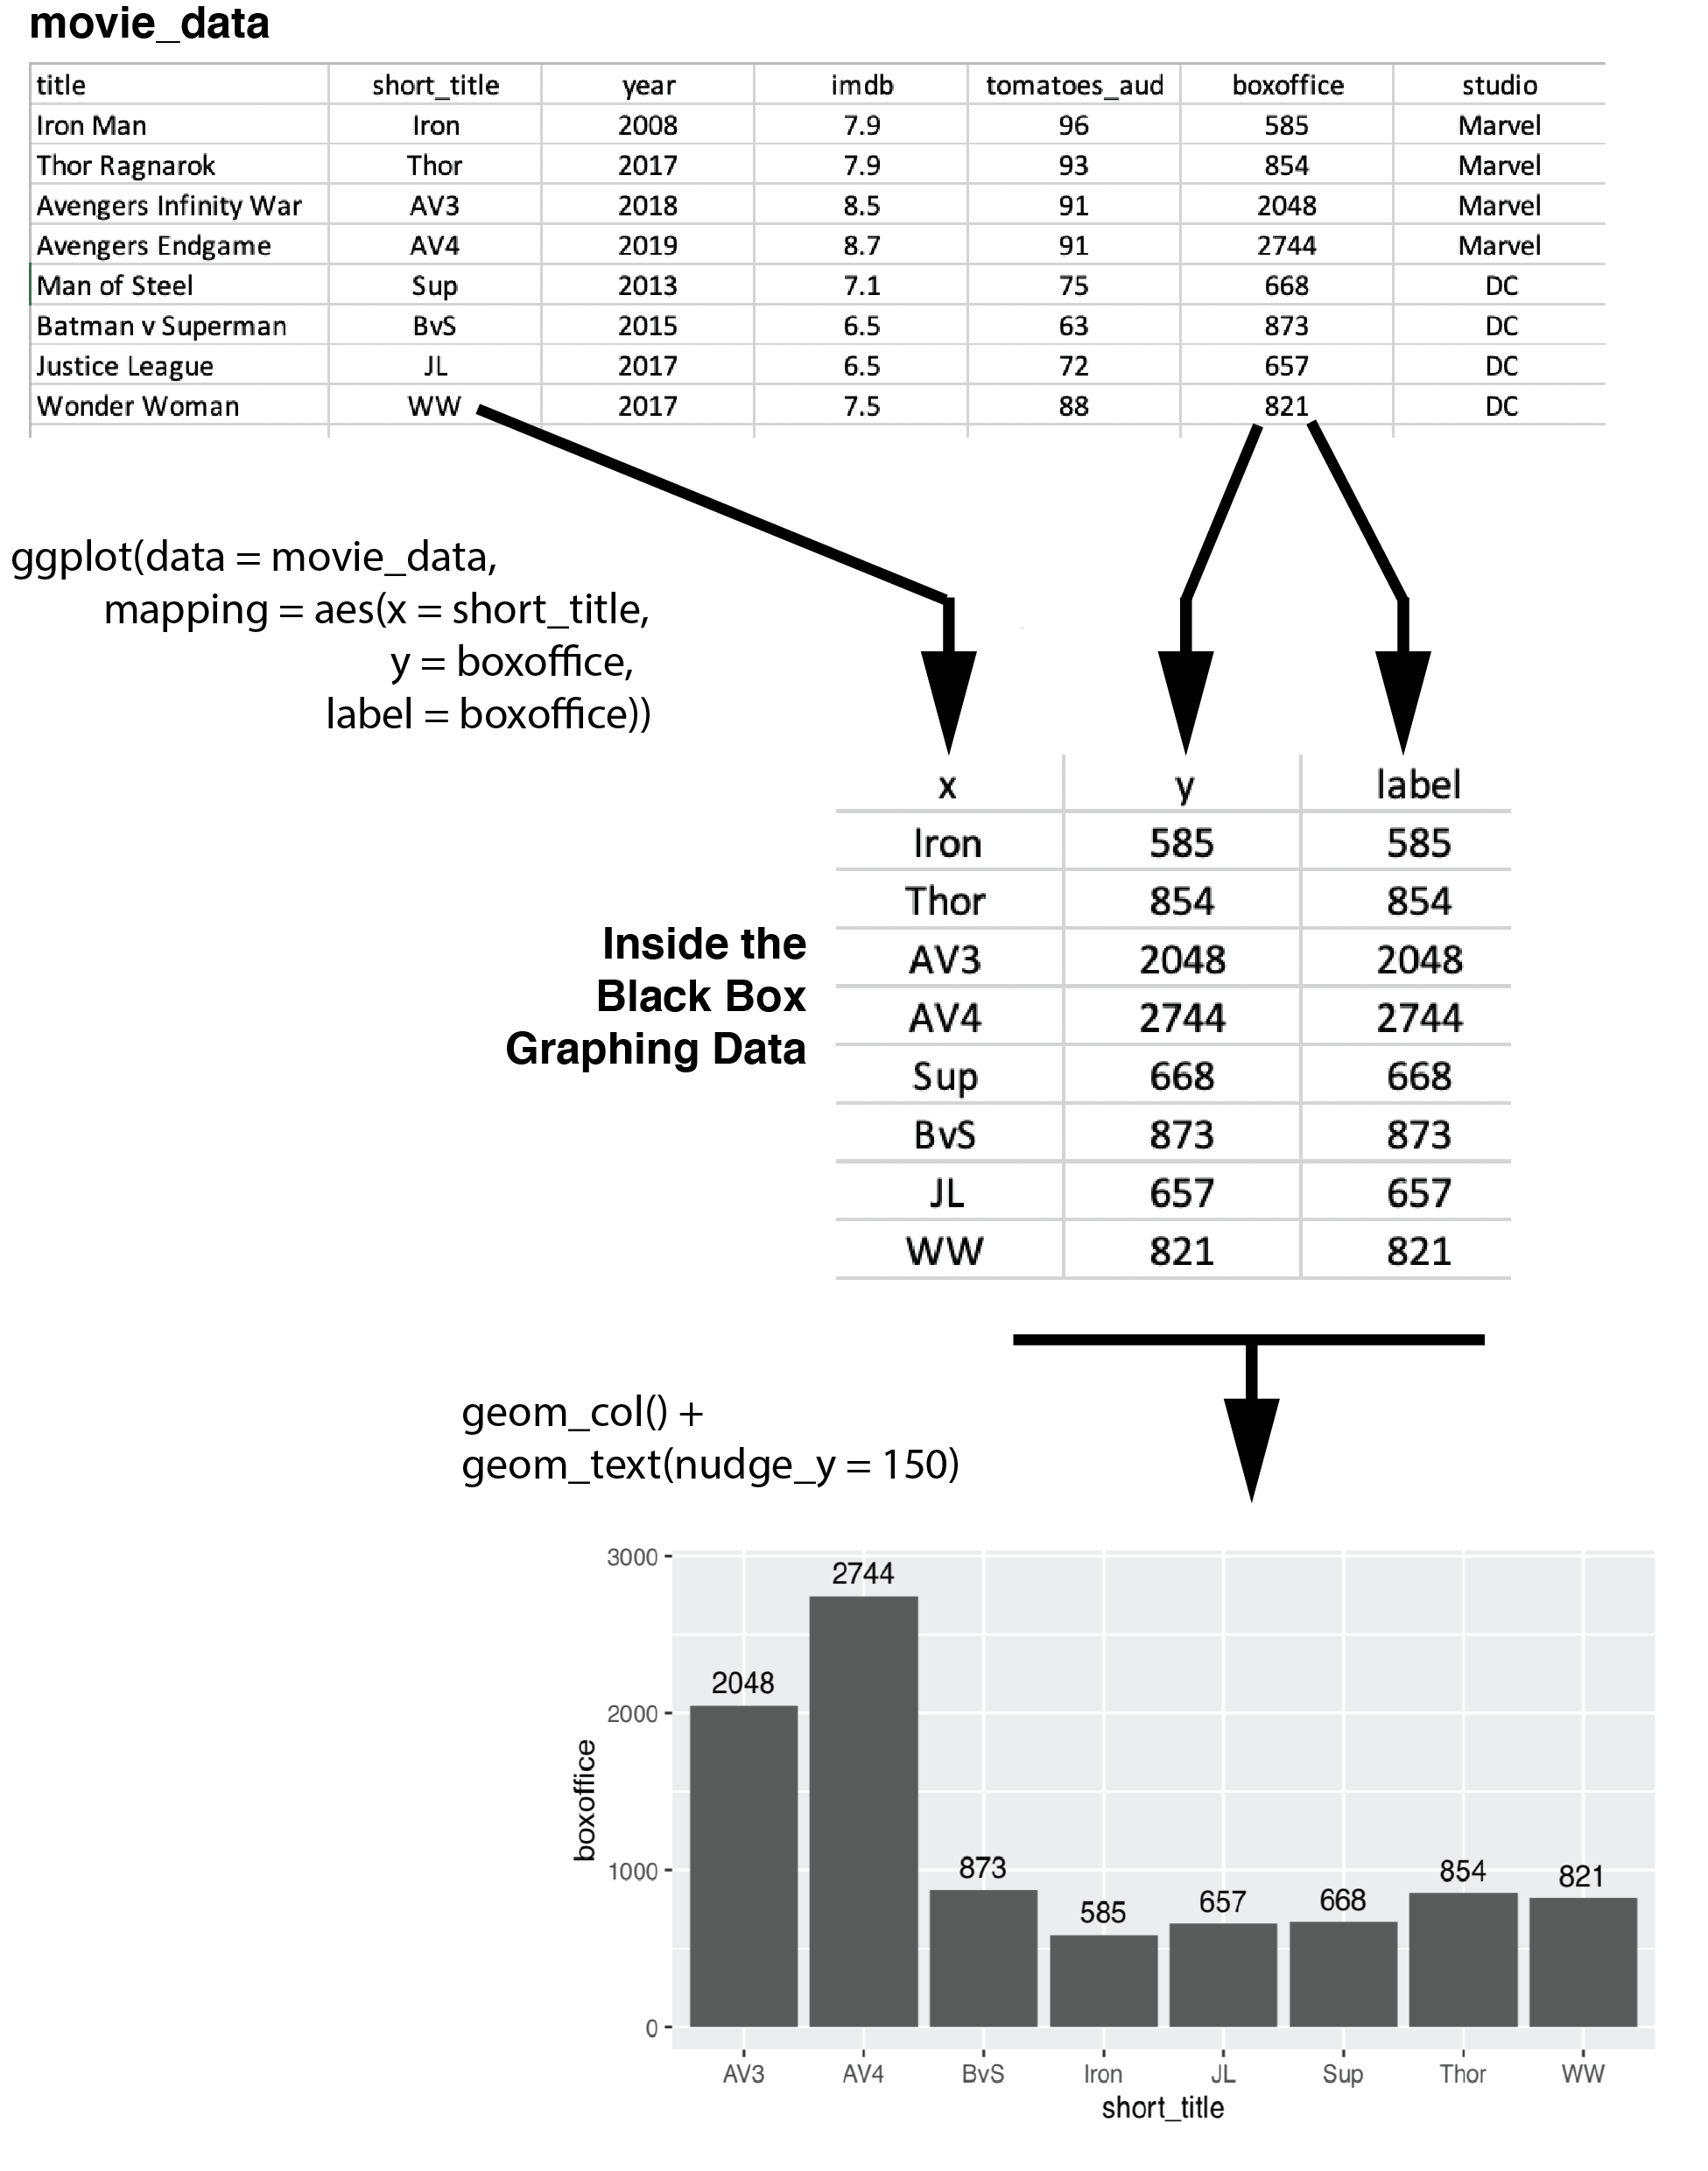
\includegraphics[width=0.7\linewidth]{ch_graphing/images/mapping} \caption{Internal data structure for ggplot}\label{fig:showmap}
\end{figure}

\hypertarget{fill-color}{%
\subsection{Fill color}\label{fill-color}}

You might want to influence the color of the bars in the graph such that the bars for Marvel and DC movies have different colors. That's easy to do with the aes() command. We simply tell aes() that the \textbf{fill} color of any object in the graph should be determined by the studio column. Simply adding ``fill = studio'' to the aes() command changes the colors of the bars -- and any other object on the graph for which fill would be relevant. The internal workings are illustrated in Figure \ref{fig:addfill}.

\begin{Shaded}
\begin{Highlighting}[]
\NormalTok{my_graph <-}\StringTok{ }\KeywordTok{ggplot}\NormalTok{(}\DataTypeTok{data =}\NormalTok{ movie_data,}
           \DataTypeTok{mapping =} \KeywordTok{aes}\NormalTok{(}\DataTypeTok{x =}\NormalTok{ short_title,}
                         \DataTypeTok{y =}\NormalTok{ boxoffice,}
                         \DataTypeTok{label =}\NormalTok{ boxoffice,}
                         \DataTypeTok{fill =}\NormalTok{ studio )) }\OperatorTok{+}
\StringTok{  }\KeywordTok{geom_col}\NormalTok{() }\OperatorTok{+}
\StringTok{  }\KeywordTok{geom_text}\NormalTok{(}\DataTypeTok{nudge_y =} \DecValTok{150}\NormalTok{) }

\KeywordTok{print}\NormalTok{(my_graph)}
\end{Highlighting}
\end{Shaded}

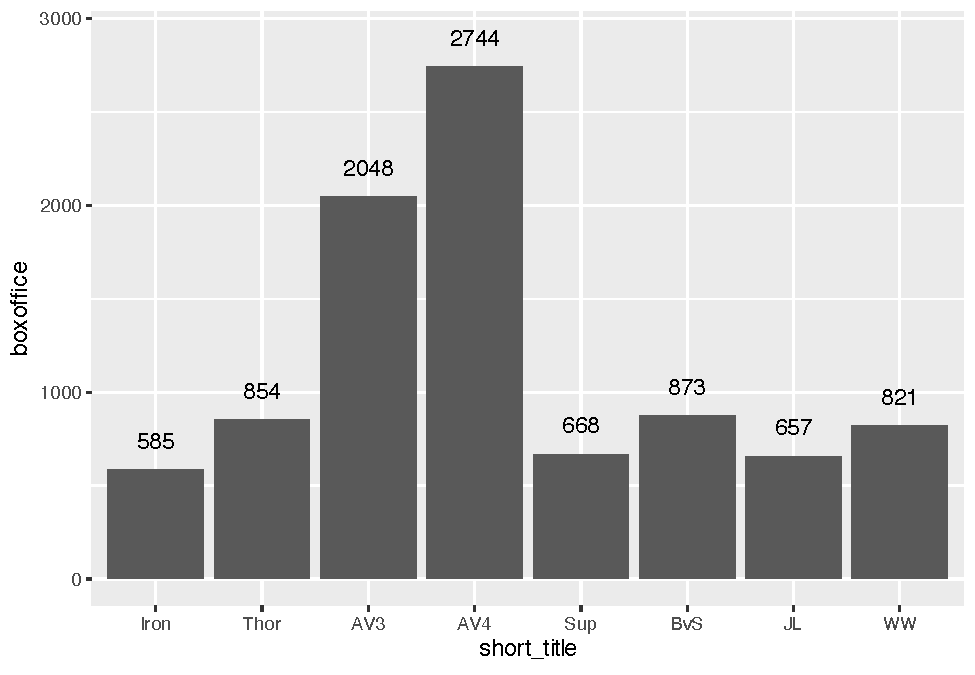
\includegraphics[width=0.65\linewidth]{bookdown_files/figure-latex/unnamed-chunk-112-1}

\begin{figure}
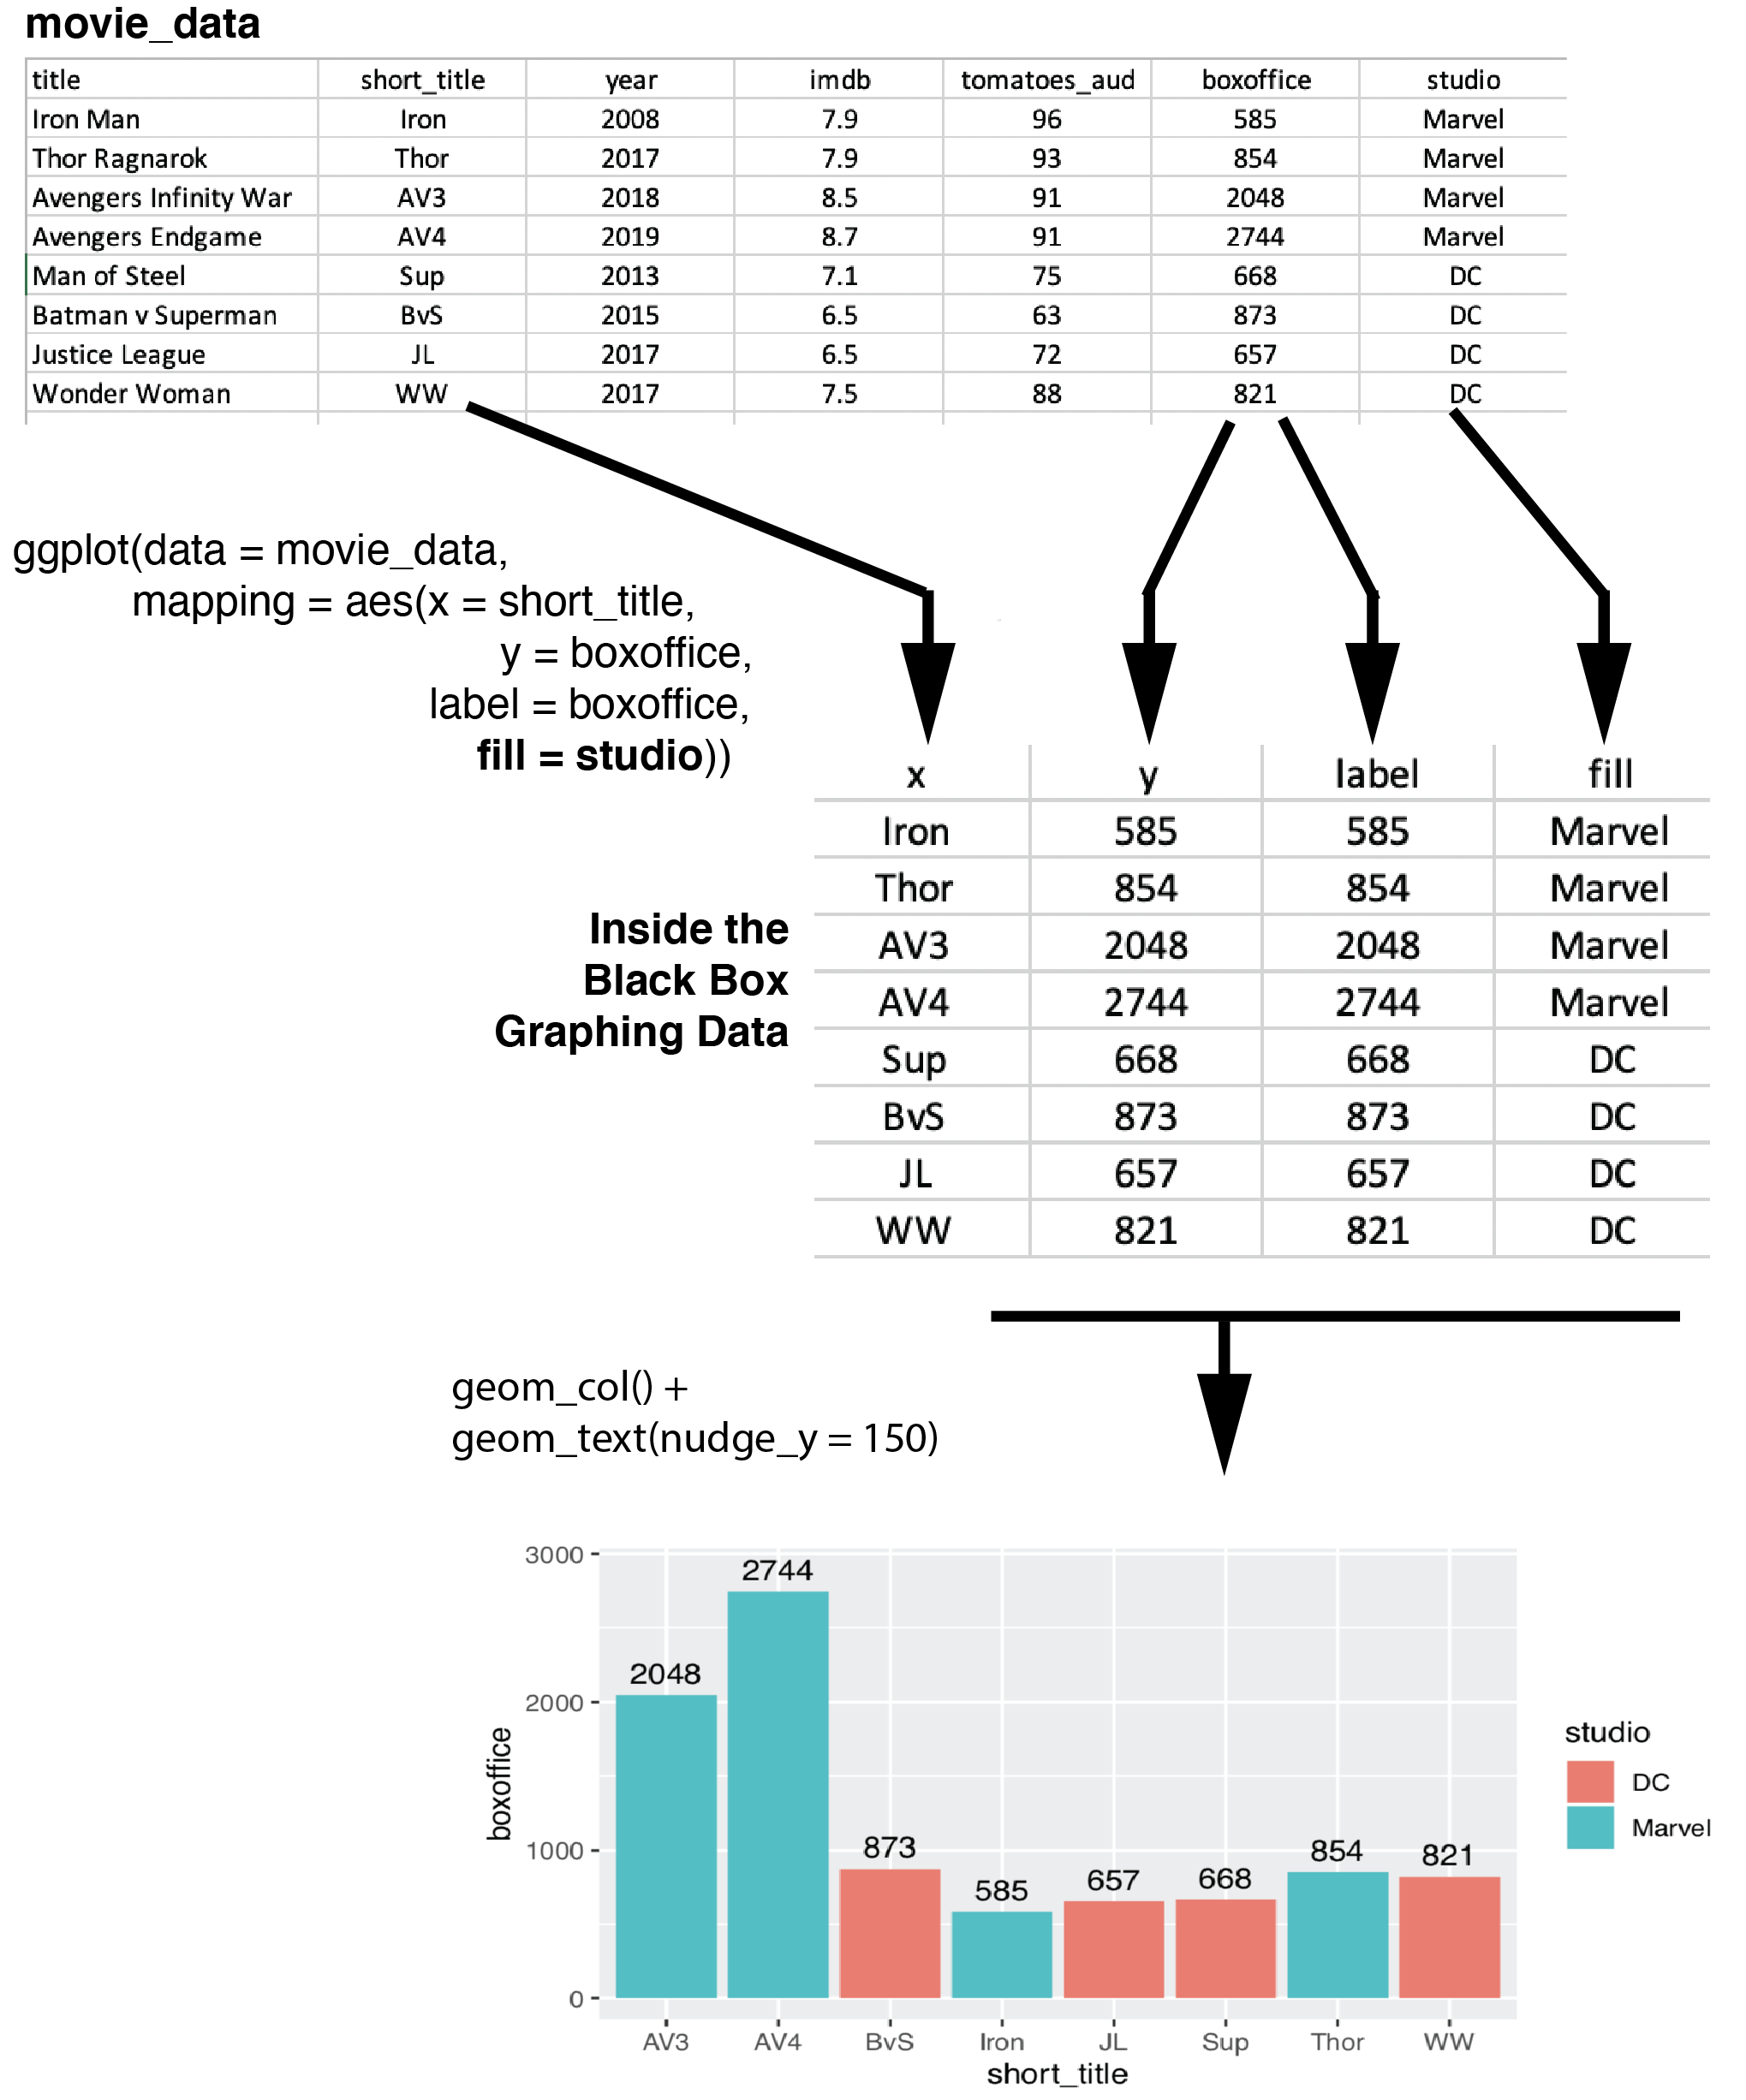
\includegraphics[width=0.7\linewidth]{ch_graphing/images/mapping_fill} \caption{Adding a fill column to the internal data}\label{fig:addfill}
\end{figure}

\hypertarget{overriding-aes}{%
\subsection{Overriding aes()}\label{overriding-aes}}

Just because you specify something in the ggplot() command doesn't mean that you are ``stuck with it'' for all your subsequent commands. Recall how at the start of this exercise we specified the data and the mapping for each geom\_col() and geom\_text() individually. We can still do that.

Now we want to add the Rotten Tomatoes Audience score for each movie above the box office revenue. But if we use geom\_text(), like we did before, it will plot the same boxoffice information because of ``label = boxoffice'' in the aes() specification within ggplot(). We want the new geom\_text() command to plot different text; that is, we want it to use ``label = tomatoes\_aud''.

Fortunately, if we simply put ``mapping = aes(label = tomatoes\_aud)'' within the new geom\_text() command we get the desired information on the graph. The mapping/aes arguments within geom\_text() override the mapping/aes arguments within ggplot(). Or more accurately, the new geom\_text() command creates its own version of the internal data set in which the label column is filled with information from tomatoes\_aud.

\begin{Shaded}
\begin{Highlighting}[]
\NormalTok{my_graph <-}\StringTok{ }\KeywordTok{ggplot}\NormalTok{(}\DataTypeTok{data =}\NormalTok{ movie_data,}
           \DataTypeTok{mapping =} \KeywordTok{aes}\NormalTok{(}\DataTypeTok{x =}\NormalTok{ short_title,}
                         \DataTypeTok{y =}\NormalTok{ boxoffice,}
                         \DataTypeTok{label =}\NormalTok{ boxoffice, }
                         \DataTypeTok{fill =}\NormalTok{ studio)) }\OperatorTok{+}
\StringTok{  }\KeywordTok{geom_col}\NormalTok{() }\OperatorTok{+}
\StringTok{  }\KeywordTok{geom_text}\NormalTok{(}\DataTypeTok{nudge_y =} \DecValTok{150}\NormalTok{)  }\OperatorTok{+}
\StringTok{  }\KeywordTok{geom_text}\NormalTok{(}\DataTypeTok{mapping =} \KeywordTok{aes}\NormalTok{(}\DataTypeTok{label =}\NormalTok{ tomatoes_aud)) }
\KeywordTok{print}\NormalTok{(my_graph)}
\end{Highlighting}
\end{Shaded}

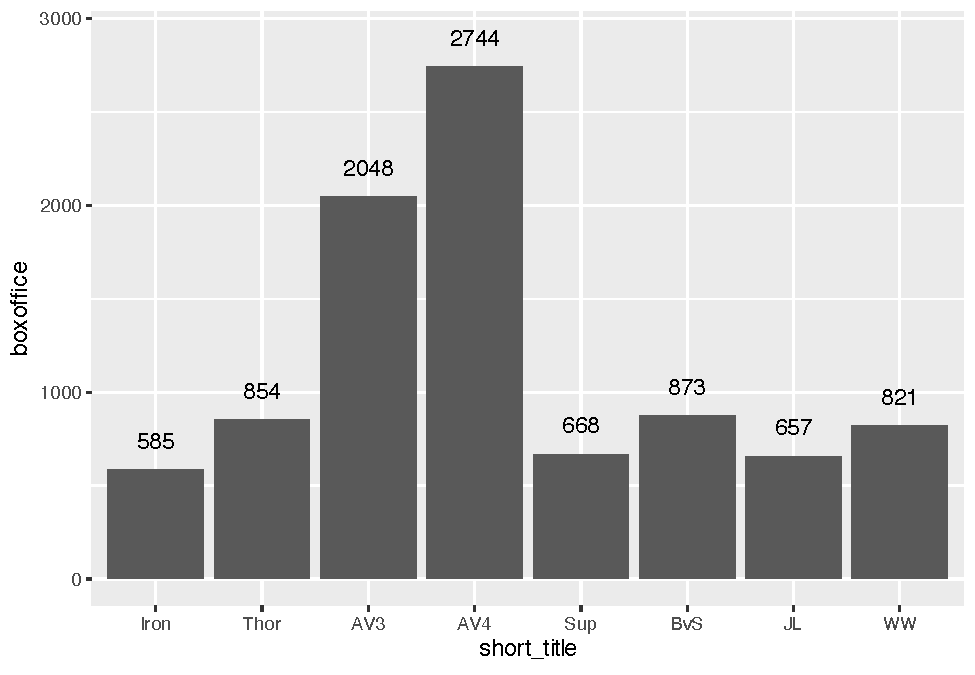
\includegraphics[width=0.65\linewidth]{bookdown_files/figure-latex/unnamed-chunk-113-1}

Notice that we have the same problem as before with the text being difficult to read because it overlaps with the bar. We add ``nudge\_y = 400'' to move the text higher than the boxoffice text/label. Don't forget the units used by nudge\_y are the units on the y-axis.

\begin{Shaded}
\begin{Highlighting}[]
\NormalTok{my_graph <-}\StringTok{ }\KeywordTok{ggplot}\NormalTok{(}\DataTypeTok{data =}\NormalTok{ movie_data,}
           \DataTypeTok{mapping =} \KeywordTok{aes}\NormalTok{(}\DataTypeTok{x =}\NormalTok{ short_title,}
                         \DataTypeTok{y =}\NormalTok{ boxoffice,}
                         \DataTypeTok{label =}\NormalTok{ boxoffice, }
                         \DataTypeTok{fill =}\NormalTok{ studio)) }\OperatorTok{+}
\StringTok{  }\KeywordTok{geom_col}\NormalTok{() }\OperatorTok{+}
\StringTok{  }\KeywordTok{geom_text}\NormalTok{(}\DataTypeTok{nudge_y =} \DecValTok{150}\NormalTok{)  }\OperatorTok{+}
\StringTok{  }\KeywordTok{geom_text}\NormalTok{(}\DataTypeTok{mapping =} \KeywordTok{aes}\NormalTok{(}\DataTypeTok{label =}\NormalTok{ tomatoes_aud), }
            \DataTypeTok{nudge_y =} \DecValTok{400}\NormalTok{) }
\KeywordTok{print}\NormalTok{(my_graph)}
\end{Highlighting}
\end{Shaded}

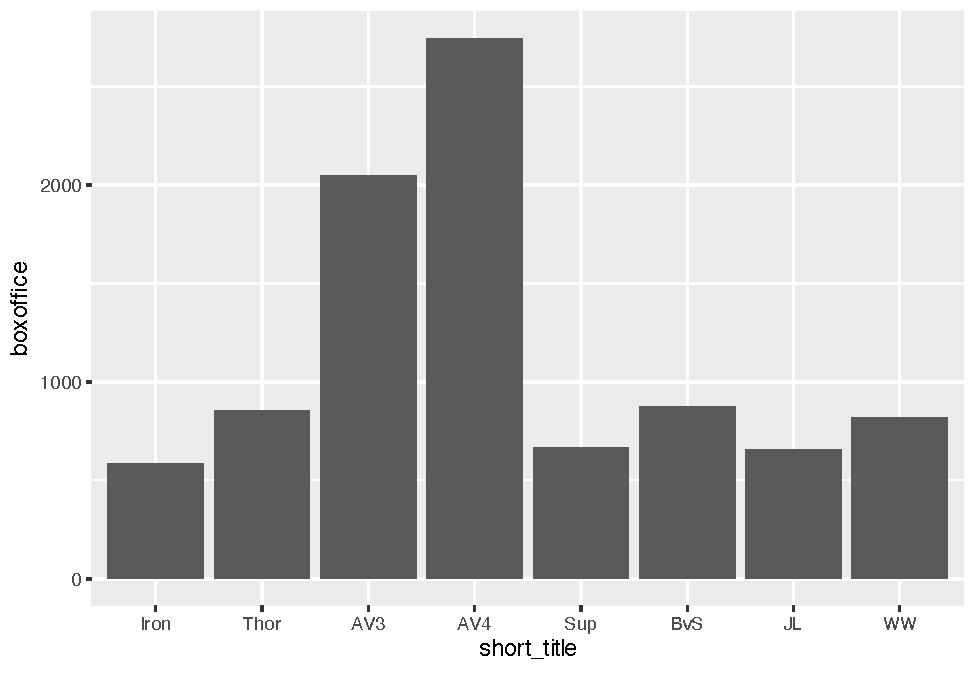
\includegraphics[width=0.65\linewidth]{bookdown_files/figure-latex/unnamed-chunk-114-1}

\newpage

\hypertarget{apa-style}{%
\section{APA style}\label{apa-style}}

Use theme\_classic() to make the graph apear in APA style. We use theme\_classic(12) to make the graph APA style with a 12-point font:

\begin{Shaded}
\begin{Highlighting}[]
\NormalTok{my_graph <-}\StringTok{ }\KeywordTok{ggplot}\NormalTok{(}\DataTypeTok{data =}\NormalTok{ movie_data,}
           \DataTypeTok{mapping =} \KeywordTok{aes}\NormalTok{(}\DataTypeTok{x =}\NormalTok{ short_title,}
                         \DataTypeTok{y =}\NormalTok{ boxoffice,}
                         \DataTypeTok{label =}\NormalTok{ boxoffice, }
                         \DataTypeTok{fill =}\NormalTok{ studio)) }\OperatorTok{+}
\StringTok{  }\KeywordTok{geom_col}\NormalTok{() }\OperatorTok{+}
\StringTok{  }\KeywordTok{geom_text}\NormalTok{(}\DataTypeTok{nudge_y =} \DecValTok{150}\NormalTok{)  }\OperatorTok{+}
\StringTok{  }\KeywordTok{geom_text}\NormalTok{(}\DataTypeTok{mapping =} \KeywordTok{aes}\NormalTok{(}\DataTypeTok{label =}\NormalTok{ tomatoes_aud), }
            \DataTypeTok{nudge_y =} \DecValTok{400}\NormalTok{) }\OperatorTok{+}
\StringTok{  }\KeywordTok{theme_classic}\NormalTok{(}\DecValTok{12}\NormalTok{)}

\KeywordTok{print}\NormalTok{(my_graph)}
\end{Highlighting}
\end{Shaded}

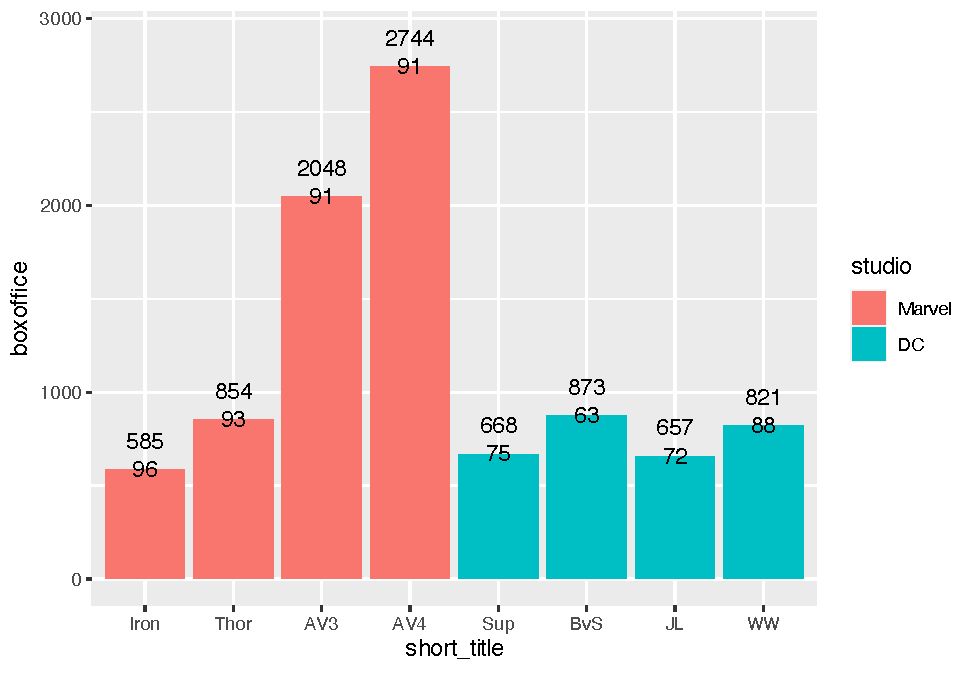
\includegraphics[width=0.65\linewidth]{bookdown_files/figure-latex/unnamed-chunk-115-1}

\hypertarget{axes}{%
\section{Axes}\label{axes}}

\hypertarget{range}{%
\subsection{Range}\label{range}}

We use the coord\_cartesian() command to adjust range of axes. In the code below we use coord\_cartesian() to make the y-axis range from 0 to 3500.

\begin{Shaded}
\begin{Highlighting}[]
\NormalTok{my_graph <-}\StringTok{ }\KeywordTok{ggplot}\NormalTok{(}\DataTypeTok{data =}\NormalTok{ movie_data,}
           \DataTypeTok{mapping =} \KeywordTok{aes}\NormalTok{(}\DataTypeTok{x =}\NormalTok{ short_title,}
                         \DataTypeTok{y =}\NormalTok{ boxoffice,}
                         \DataTypeTok{label =}\NormalTok{ boxoffice, }
                         \DataTypeTok{fill =}\NormalTok{ studio)) }\OperatorTok{+}
\StringTok{  }\KeywordTok{geom_col}\NormalTok{() }\OperatorTok{+}
\StringTok{  }\KeywordTok{geom_text}\NormalTok{(}\DataTypeTok{nudge_y =} \DecValTok{150}\NormalTok{)  }\OperatorTok{+}
\StringTok{  }\KeywordTok{geom_text}\NormalTok{(}\DataTypeTok{mapping =} \KeywordTok{aes}\NormalTok{(}\DataTypeTok{label =}\NormalTok{ tomatoes_aud), }
            \DataTypeTok{nudge_y =} \DecValTok{400}\NormalTok{) }\OperatorTok{+}
\StringTok{  }\KeywordTok{coord_cartesian}\NormalTok{(}\DataTypeTok{ylim =} \KeywordTok{c}\NormalTok{(}\DecValTok{0}\NormalTok{, }\DecValTok{3500}\NormalTok{)) }\OperatorTok{+}
\StringTok{  }\KeywordTok{theme_classic}\NormalTok{(}\DecValTok{12}\NormalTok{)}


\KeywordTok{print}\NormalTok{(my_graph)}
\end{Highlighting}
\end{Shaded}

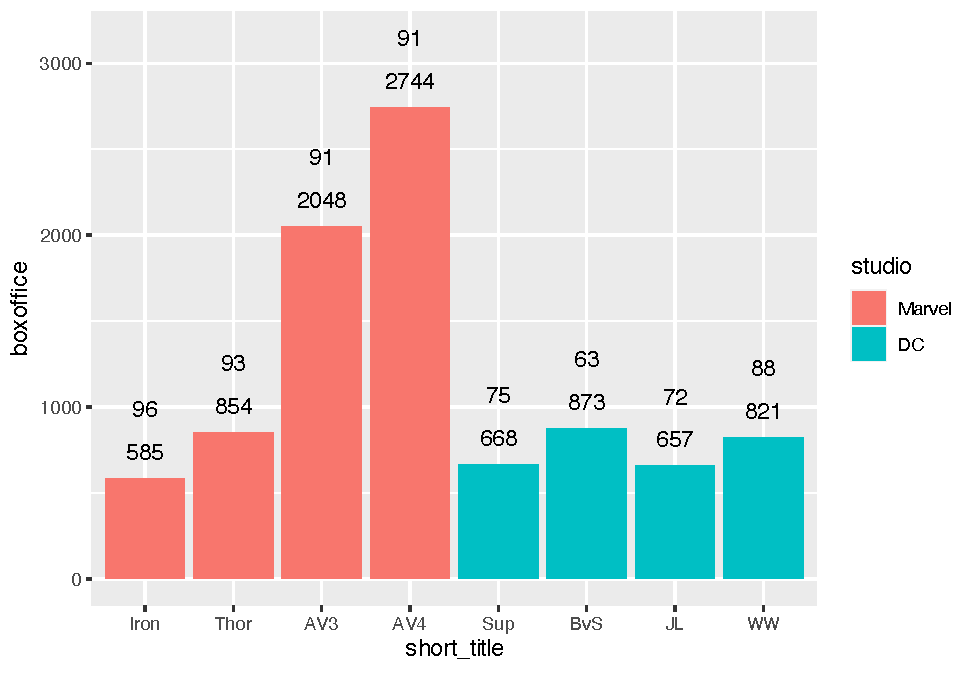
\includegraphics[width=0.65\linewidth]{bookdown_files/figure-latex/unnamed-chunk-116-1}

Note that if you had a continuous variable on the x-axis (we do not in this example), you could set the range of both the x- and y-axes like this:

\begin{Shaded}
\begin{Highlighting}[]
\KeywordTok{coord_cartesian}\NormalTok{(}\DataTypeTok{ylim =} \KeywordTok{c}\NormalTok{(}\DecValTok{0}\NormalTok{, }\DecValTok{3500}\NormalTok{),}
                \DataTypeTok{xlim =} \KeywordTok{c}\NormalTok{(}\DecValTok{0}\NormalTok{, }\DecValTok{3500}\NormalTok{))}
\end{Highlighting}
\end{Shaded}

\hypertarget{ticks}{%
\subsection{Ticks}\label{ticks}}

We use the scale\_y\_continuous() command to adjust the ticks on the y-axis. We set the ticks on the y-axis to range from 0 to 3500 in 500 tick increments using the scale\_y\_continuous command below via the breaks argument:

\begin{Shaded}
\begin{Highlighting}[]
\NormalTok{my_graph <-}\StringTok{ }\KeywordTok{ggplot}\NormalTok{(}\DataTypeTok{data =}\NormalTok{ movie_data,}
           \DataTypeTok{mapping =} \KeywordTok{aes}\NormalTok{(}\DataTypeTok{x =}\NormalTok{ short_title,}
                         \DataTypeTok{y =}\NormalTok{ boxoffice,}
                         \DataTypeTok{label =}\NormalTok{ boxoffice, }
                         \DataTypeTok{fill =}\NormalTok{ studio)) }\OperatorTok{+}
\StringTok{  }\KeywordTok{geom_col}\NormalTok{() }\OperatorTok{+}
\StringTok{  }\KeywordTok{geom_text}\NormalTok{(}\DataTypeTok{nudge_y =} \DecValTok{150}\NormalTok{)  }\OperatorTok{+}
\StringTok{  }\KeywordTok{geom_text}\NormalTok{(}\DataTypeTok{mapping =} \KeywordTok{aes}\NormalTok{(}\DataTypeTok{label =}\NormalTok{ tomatoes_aud), }
            \DataTypeTok{nudge_y =} \DecValTok{400}\NormalTok{) }\OperatorTok{+}
\StringTok{  }\KeywordTok{coord_cartesian}\NormalTok{(}\DataTypeTok{ylim =} \KeywordTok{c}\NormalTok{(}\DecValTok{0}\NormalTok{, }\DecValTok{3500}\NormalTok{)) }\OperatorTok{+}
\StringTok{  }\KeywordTok{scale_y_continuous}\NormalTok{(}\DataTypeTok{breaks =} \KeywordTok{seq}\NormalTok{(}\DecValTok{0}\NormalTok{, }\DecValTok{3500}\NormalTok{, }\DataTypeTok{by =} \DecValTok{500}\NormalTok{)) }\OperatorTok{+}
\StringTok{  }\KeywordTok{theme_classic}\NormalTok{(}\DecValTok{12}\NormalTok{)}

\KeywordTok{print}\NormalTok{(my_graph)}
\end{Highlighting}
\end{Shaded}

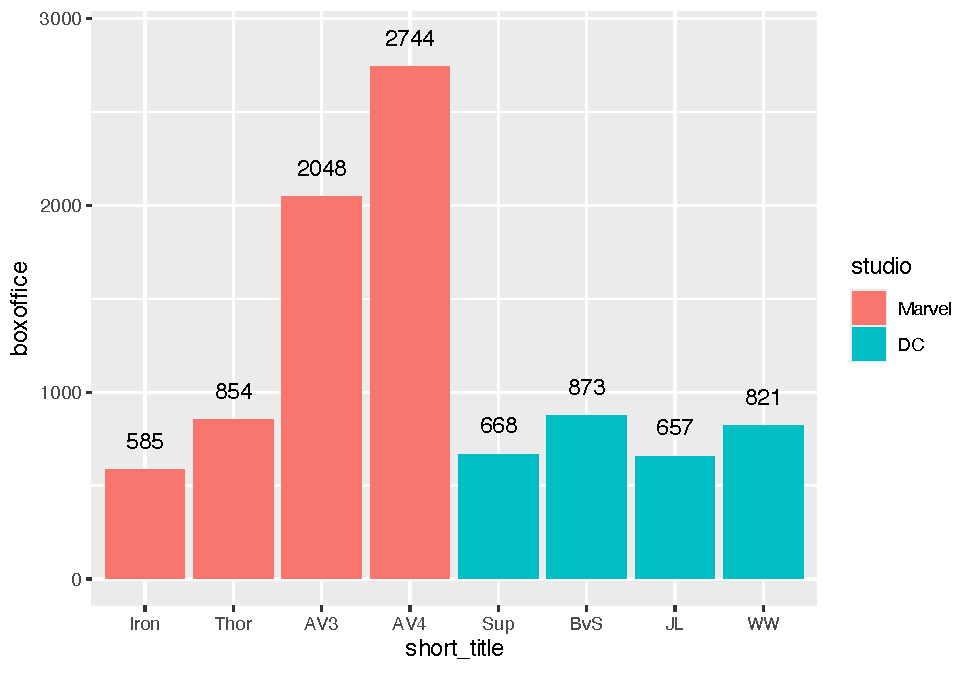
\includegraphics[width=0.65\linewidth]{bookdown_files/figure-latex/unnamed-chunk-118-1}

Note that if you had a continuous variable on the x-axis (we do not in this example), you could set the ticks of the x-axis like the code below using scale\_x\_continuous:

\begin{Shaded}
\begin{Highlighting}[]
\KeywordTok{scale_x_continuous}\NormalTok{(}\DataTypeTok{breaks =} \KeywordTok{seq}\NormalTok{(}\DecValTok{0}\NormalTok{, }\DecValTok{3500}\NormalTok{, }\DataTypeTok{by =} \DecValTok{500}\NormalTok{))}
\end{Highlighting}
\end{Shaded}

\hypertarget{labels}{%
\subsection{Labels}\label{labels}}

Labels are an extremely important part of any graph. This fact is the focus of the \href{https://xkcd.com/833/}{xkcd} cartoon below:

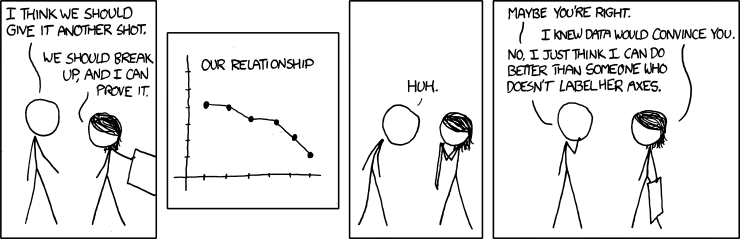
\includegraphics[width=0.8\linewidth]{ch_graphing/images/convincing}

We use the labs() command to set the labels for the x- and y-axes:

\begin{Shaded}
\begin{Highlighting}[]
\NormalTok{my_graph <-}\StringTok{ }\KeywordTok{ggplot}\NormalTok{(}\DataTypeTok{data =}\NormalTok{ movie_data,}
           \DataTypeTok{mapping =} \KeywordTok{aes}\NormalTok{(}\DataTypeTok{x =}\NormalTok{ short_title,}
                         \DataTypeTok{y =}\NormalTok{ boxoffice,}
                         \DataTypeTok{label =}\NormalTok{ boxoffice, }
                         \DataTypeTok{fill =}\NormalTok{ studio)) }\OperatorTok{+}
\StringTok{  }\KeywordTok{geom_col}\NormalTok{() }\OperatorTok{+}
\StringTok{  }\KeywordTok{geom_text}\NormalTok{(}\DataTypeTok{nudge_y =} \DecValTok{150}\NormalTok{)  }\OperatorTok{+}
\StringTok{  }\KeywordTok{geom_text}\NormalTok{(}\DataTypeTok{mapping =} \KeywordTok{aes}\NormalTok{(}\DataTypeTok{label =}\NormalTok{ tomatoes_aud), }
            \DataTypeTok{nudge_y =} \DecValTok{400}\NormalTok{) }\OperatorTok{+}
\StringTok{  }\KeywordTok{coord_cartesian}\NormalTok{(}\DataTypeTok{ylim =} \KeywordTok{c}\NormalTok{(}\DecValTok{0}\NormalTok{, }\DecValTok{3500}\NormalTok{)) }\OperatorTok{+}
\StringTok{  }\KeywordTok{scale_y_continuous}\NormalTok{(}\DataTypeTok{breaks =} \KeywordTok{seq}\NormalTok{(}\DecValTok{0}\NormalTok{, }\DecValTok{3500}\NormalTok{, }\DataTypeTok{by =} \DecValTok{500}\NormalTok{)) }\OperatorTok{+}
\StringTok{  }\KeywordTok{labs}\NormalTok{(}\DataTypeTok{x =} \StringTok{"Movie"}\NormalTok{,}
       \DataTypeTok{y =} \StringTok{"Box office (millions)"}\NormalTok{,}
       \DataTypeTok{fill =} \StringTok{"Studio"}\NormalTok{) }\OperatorTok{+}
\StringTok{  }\KeywordTok{theme_classic}\NormalTok{(}\DecValTok{12}\NormalTok{)}

\KeywordTok{print}\NormalTok{(my_graph)}
\end{Highlighting}
\end{Shaded}

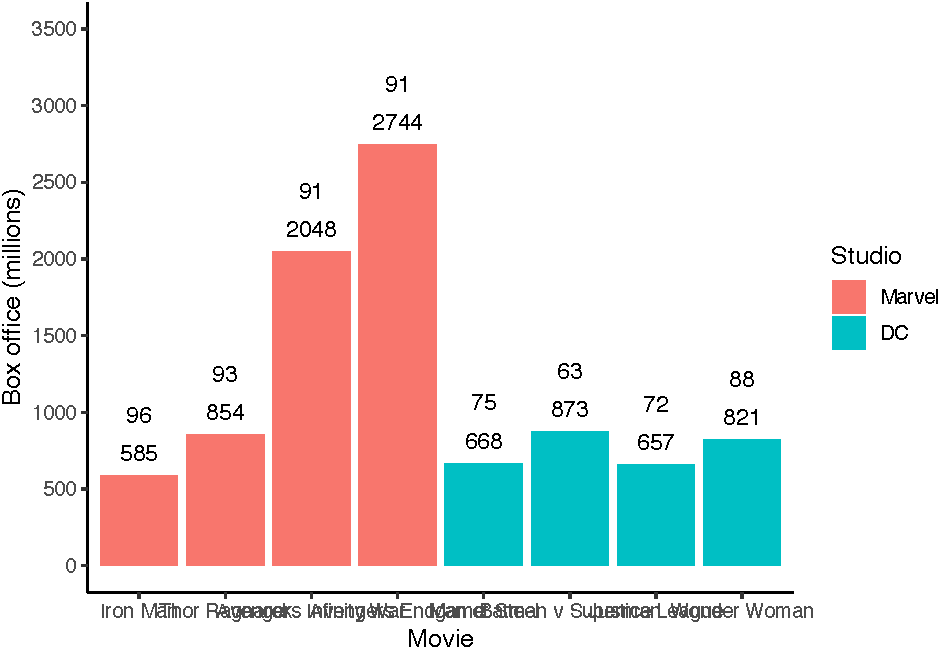
\includegraphics[width=0.65\linewidth]{bookdown_files/figure-latex/unnamed-chunk-121-1}

\hypertarget{axis-values}{%
\section{Axis values}\label{axis-values}}

\hypertarget{text}{%
\subsection{Text}\label{text}}

What if we want to use the full movie title rather than the short version on the x-axis of the graph? That is, you want to change the values along the x-axis. Two methods are presented below.

\hypertarget{method-1-recoding-axis-values}{%
\subsubsection{Method 1: Recoding axis values}\label{method-1-recoding-axis-values}}

Our data file contains a column with the long/full version of the movie names. But many times you won't have the additional/longer labels available in this manner. In this situation, you use the scale\_x\_discrete() command to change the values along the x-axis.

The values along the x-axis come from the short\_title column which is a factor. The levels of that factor correspond to the short titles for the movies (Iron, Thor, etc.). We need to relabel the levels of the short\_title factor to get a graph with full titles. We relabel the levels of the short\_title factor using the scale\_x\_discrete() command. The graph code with scale\_x\_discrete() command is below - notice the problem we have with the labels overlapping though. On the next page, we'll use an easier approach though - since we have an extra column with the full titles.

\begin{Shaded}
\begin{Highlighting}[]
\NormalTok{my_graph <-}\StringTok{ }\KeywordTok{ggplot}\NormalTok{(}\DataTypeTok{data =}\NormalTok{ movie_data,}
           \DataTypeTok{mapping =} \KeywordTok{aes}\NormalTok{(}\DataTypeTok{x =}\NormalTok{ short_title,}
                         \DataTypeTok{y =}\NormalTok{ boxoffice,}
                         \DataTypeTok{label =}\NormalTok{ boxoffice, }
                         \DataTypeTok{fill =}\NormalTok{ studio)) }\OperatorTok{+}
\StringTok{  }\KeywordTok{geom_col}\NormalTok{() }\OperatorTok{+}
\StringTok{  }\KeywordTok{geom_text}\NormalTok{(}\DataTypeTok{nudge_y =} \DecValTok{150}\NormalTok{)  }\OperatorTok{+}
\StringTok{  }\KeywordTok{geom_text}\NormalTok{(}\DataTypeTok{mapping =} \KeywordTok{aes}\NormalTok{(}\DataTypeTok{label =}\NormalTok{ tomatoes_aud), }
            \DataTypeTok{nudge_y =} \DecValTok{400}\NormalTok{) }\OperatorTok{+}
\StringTok{  }\KeywordTok{coord_cartesian}\NormalTok{(}\DataTypeTok{ylim =} \KeywordTok{c}\NormalTok{(}\DecValTok{0}\NormalTok{, }\DecValTok{3500}\NormalTok{)) }\OperatorTok{+}
\StringTok{  }\KeywordTok{scale_y_continuous}\NormalTok{(}\DataTypeTok{breaks =} \KeywordTok{seq}\NormalTok{(}\DecValTok{0}\NormalTok{, }\DecValTok{3500}\NormalTok{, }\DataTypeTok{by =} \DecValTok{500}\NormalTok{)) }\OperatorTok{+}
\StringTok{  }\KeywordTok{scale_x_discrete}\NormalTok{(}\DataTypeTok{labels=}\KeywordTok{c}\NormalTok{(}\StringTok{"Iron"}\NormalTok{ =}\StringTok{ "Iron Man"}\NormalTok{, }
                            \StringTok{"Thor"}\NormalTok{ =}\StringTok{ "Thor Ragnarkok"}\NormalTok{,}
                            \StringTok{"AV3"}\NormalTok{ =}\StringTok{ "Avengers Infinity War"}\NormalTok{,}
                            \StringTok{"AV4"}\NormalTok{ =}\StringTok{ "Avengers Endgame"}\NormalTok{,}
                            \StringTok{"Sup"}\NormalTok{ =}\StringTok{ "Man of Steel"}\NormalTok{,}
                            \StringTok{"BvS"}\NormalTok{ =}\StringTok{ "Batman v Superman"}\NormalTok{,}
                            \StringTok{"JL"}\NormalTok{ =}\StringTok{ "Justice League"}\NormalTok{,}
                            \StringTok{"WW"}\NormalTok{ =}\StringTok{ "Wonder Woman"}\NormalTok{)) }\OperatorTok{+}
\StringTok{  }\KeywordTok{labs}\NormalTok{(}\DataTypeTok{x =} \StringTok{"Movie"}\NormalTok{,}
       \DataTypeTok{y =} \StringTok{"Box office (millions)"}\NormalTok{,}
       \DataTypeTok{fill =} \StringTok{"Studio"}\NormalTok{) }\OperatorTok{+}
\StringTok{  }\KeywordTok{theme_classic}\NormalTok{(}\DecValTok{12}\NormalTok{)}
  

\KeywordTok{print}\NormalTok{(my_graph)}
\end{Highlighting}
\end{Shaded}

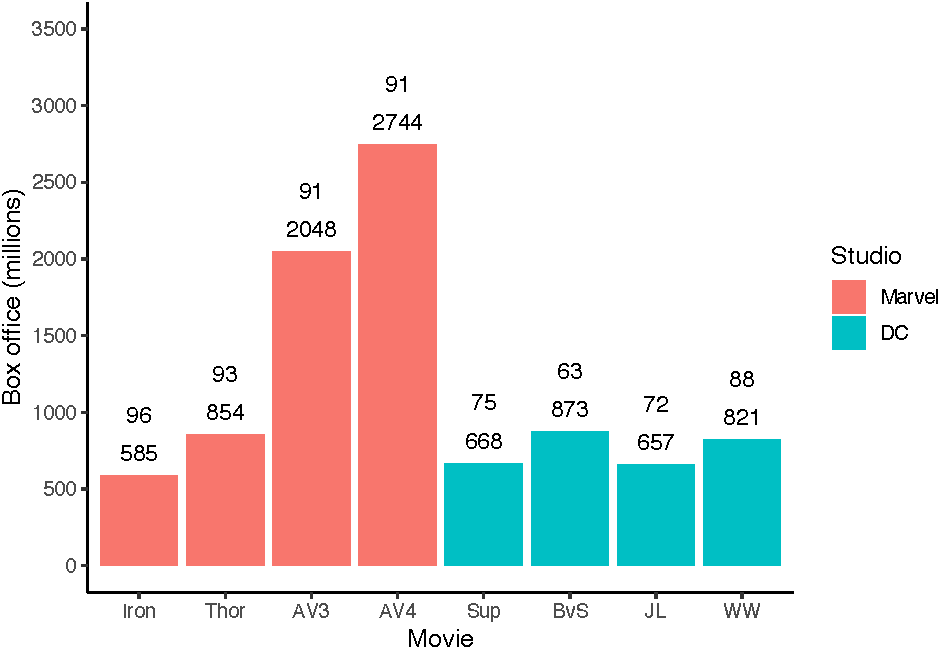
\includegraphics[width=0.65\linewidth]{bookdown_files/figure-latex/unnamed-chunk-122-1}

\hypertarget{method-2-longer-label-columns}{%
\subsubsection{Method 2: Longer label columns}\label{method-2-longer-label-columns}}

With our movie data we don't need to use scale\_x\_discrete() because we have a column in the data with the full titles. Consequently, to use full length titles we just have to change the \emph{mapping}for x from short\_title to title. Notice that we still have the problem with overlapping labels on the x-axis!

\begin{Shaded}
\begin{Highlighting}[]
\NormalTok{my_graph <-}\StringTok{ }\KeywordTok{ggplot}\NormalTok{(}\DataTypeTok{data =}\NormalTok{ movie_data,}
           \DataTypeTok{mapping =} \KeywordTok{aes}\NormalTok{(}\DataTypeTok{x =}\NormalTok{ title,}
                         \DataTypeTok{y =}\NormalTok{ boxoffice,}
                         \DataTypeTok{label =}\NormalTok{ boxoffice, }
                         \DataTypeTok{fill =}\NormalTok{ studio)) }\OperatorTok{+}
\StringTok{  }\KeywordTok{geom_col}\NormalTok{() }\OperatorTok{+}
\StringTok{  }\KeywordTok{geom_text}\NormalTok{(}\DataTypeTok{nudge_y =} \DecValTok{150}\NormalTok{)  }\OperatorTok{+}
\StringTok{  }\KeywordTok{geom_text}\NormalTok{(}\DataTypeTok{mapping =} \KeywordTok{aes}\NormalTok{(}\DataTypeTok{label =}\NormalTok{ tomatoes_aud), }
            \DataTypeTok{nudge_y =} \DecValTok{400}\NormalTok{) }\OperatorTok{+}
\StringTok{  }\KeywordTok{coord_cartesian}\NormalTok{(}\DataTypeTok{ylim =} \KeywordTok{c}\NormalTok{(}\DecValTok{0}\NormalTok{, }\DecValTok{3500}\NormalTok{)) }\OperatorTok{+}
\StringTok{  }\KeywordTok{scale_y_continuous}\NormalTok{(}\DataTypeTok{breaks =} \KeywordTok{seq}\NormalTok{(}\DecValTok{0}\NormalTok{, }\DecValTok{3500}\NormalTok{, }\DataTypeTok{by =} \DecValTok{500}\NormalTok{)) }\OperatorTok{+}
\StringTok{  }\KeywordTok{labs}\NormalTok{(}\DataTypeTok{x =} \StringTok{"Movie"}\NormalTok{,}
       \DataTypeTok{y =} \StringTok{"Box office (millions)"}\NormalTok{,}
       \DataTypeTok{fill =} \StringTok{"Studio"}\NormalTok{) }\OperatorTok{+}
\StringTok{  }\KeywordTok{theme_classic}\NormalTok{(}\DecValTok{12}\NormalTok{)}
  

\KeywordTok{print}\NormalTok{(my_graph)}
\end{Highlighting}
\end{Shaded}

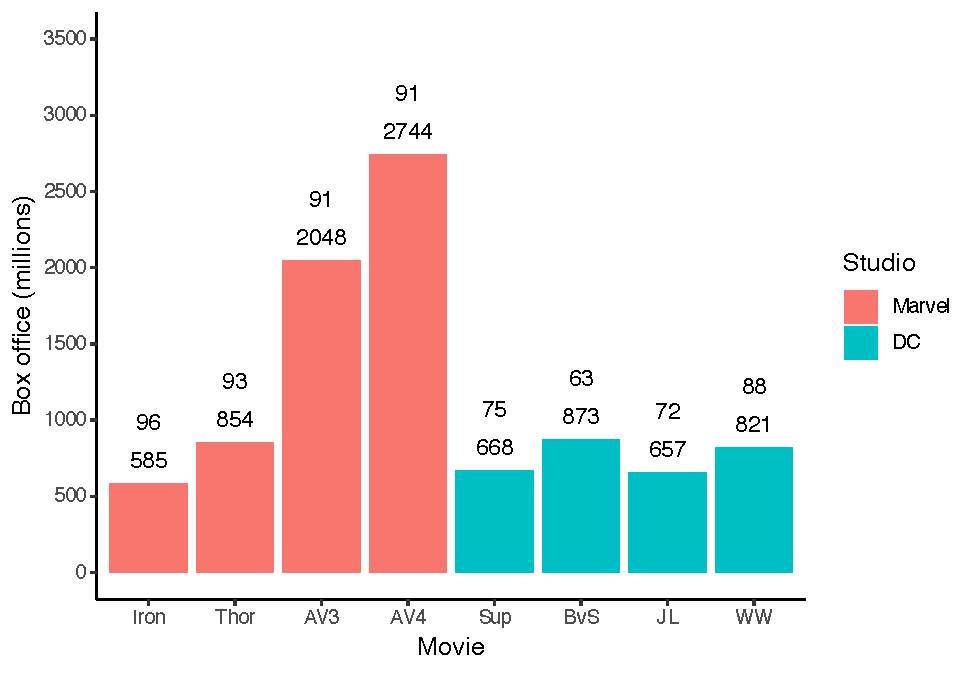
\includegraphics[width=0.65\linewidth]{bookdown_files/figure-latex/unnamed-chunk-123-1}

\hypertarget{angle}{%
\subsection{Angle}\label{angle}}

Use theme() to adjust the angle of x-axis labels. Notice, however, that the longer titles are vertically centered on each point on the x-axis. In the next section we fix this problem.

\textbf{Important}: The theme command must come after the theme\_classic command. Otherwise, theme\_classic will undo the work done by the theme\_command if it appears after the theme command.

\begin{Shaded}
\begin{Highlighting}[]
\NormalTok{my_graph <-}\StringTok{ }\KeywordTok{ggplot}\NormalTok{(}\DataTypeTok{data =}\NormalTok{ movie_data,}
           \DataTypeTok{mapping =} \KeywordTok{aes}\NormalTok{(}\DataTypeTok{x =}\NormalTok{ title,}
                         \DataTypeTok{y =}\NormalTok{ boxoffice,}
                         \DataTypeTok{label =}\NormalTok{ boxoffice, }
                         \DataTypeTok{fill =}\NormalTok{ studio)) }\OperatorTok{+}
\StringTok{  }\KeywordTok{geom_col}\NormalTok{() }\OperatorTok{+}
\StringTok{  }\KeywordTok{geom_text}\NormalTok{(}\DataTypeTok{nudge_y =} \DecValTok{150}\NormalTok{)  }\OperatorTok{+}
\StringTok{  }\KeywordTok{geom_text}\NormalTok{(}\DataTypeTok{mapping =} \KeywordTok{aes}\NormalTok{(}\DataTypeTok{label =}\NormalTok{ tomatoes_aud), }
            \DataTypeTok{nudge_y =} \DecValTok{400}\NormalTok{) }\OperatorTok{+}
\StringTok{  }\KeywordTok{coord_cartesian}\NormalTok{(}\DataTypeTok{ylim =} \KeywordTok{c}\NormalTok{(}\DecValTok{0}\NormalTok{, }\DecValTok{3500}\NormalTok{)) }\OperatorTok{+}
\StringTok{  }\KeywordTok{scale_y_continuous}\NormalTok{(}\DataTypeTok{breaks =} \KeywordTok{seq}\NormalTok{(}\DecValTok{0}\NormalTok{, }\DecValTok{3500}\NormalTok{, }\DataTypeTok{by =} \DecValTok{500}\NormalTok{)) }\OperatorTok{+}
\StringTok{  }\KeywordTok{labs}\NormalTok{(}\DataTypeTok{x =} \StringTok{"Movie"}\NormalTok{,}
       \DataTypeTok{y =} \StringTok{"Box office (millions)"}\NormalTok{,}
       \DataTypeTok{fill =} \StringTok{"Studio"}\NormalTok{) }\OperatorTok{+}
\StringTok{  }\KeywordTok{theme_classic}\NormalTok{(}\DecValTok{12}\NormalTok{) }\OperatorTok{+}
\StringTok{  }\KeywordTok{theme}\NormalTok{(}\DataTypeTok{axis.text.x =} \KeywordTok{element_text}\NormalTok{(}\DataTypeTok{angle =} \DecValTok{60}\NormalTok{))}

\KeywordTok{print}\NormalTok{(my_graph)}
\end{Highlighting}
\end{Shaded}

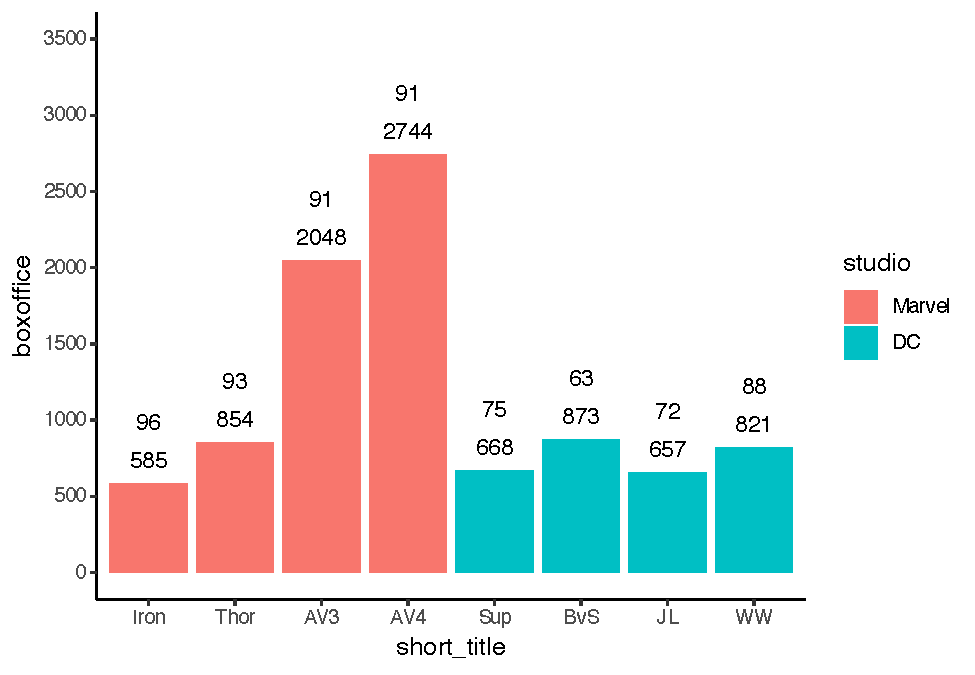
\includegraphics[width=0.65\linewidth]{bookdown_files/figure-latex/unnamed-chunk-124-1}

\hypertarget{alignment}{%
\subsection{Alignment}\label{alignment}}

Use theme() and the hjust argument to adjust the alignment of the x-axis labels. To make the titles look correct on the x-axis we need them at an angle, but we also need them right justified against the x-axis. We do that with the the hjust argument (1 means right justify). See the code below:

\begin{Shaded}
\begin{Highlighting}[]
\NormalTok{my_graph <-}\StringTok{ }\KeywordTok{ggplot}\NormalTok{(}\DataTypeTok{data =}\NormalTok{ movie_data,}
           \DataTypeTok{mapping =} \KeywordTok{aes}\NormalTok{(}\DataTypeTok{x =}\NormalTok{ title,}
                         \DataTypeTok{y =}\NormalTok{ boxoffice,}
                         \DataTypeTok{label =}\NormalTok{ boxoffice, }
                         \DataTypeTok{fill =}\NormalTok{ studio)) }\OperatorTok{+}
\StringTok{  }\KeywordTok{geom_col}\NormalTok{() }\OperatorTok{+}
\StringTok{  }\KeywordTok{geom_text}\NormalTok{(}\DataTypeTok{nudge_y =} \DecValTok{150}\NormalTok{)  }\OperatorTok{+}
\StringTok{  }\KeywordTok{geom_text}\NormalTok{(}\DataTypeTok{mapping =} \KeywordTok{aes}\NormalTok{(}\DataTypeTok{label =}\NormalTok{ tomatoes_aud), }
            \DataTypeTok{nudge_y =} \DecValTok{400}\NormalTok{) }\OperatorTok{+}
\StringTok{  }\KeywordTok{coord_cartesian}\NormalTok{(}\DataTypeTok{ylim =} \KeywordTok{c}\NormalTok{(}\DecValTok{0}\NormalTok{, }\DecValTok{3500}\NormalTok{)) }\OperatorTok{+}
\StringTok{  }\KeywordTok{scale_y_continuous}\NormalTok{(}\DataTypeTok{breaks =} \KeywordTok{seq}\NormalTok{(}\DecValTok{0}\NormalTok{, }\DecValTok{3500}\NormalTok{, }\DataTypeTok{by =} \DecValTok{500}\NormalTok{)) }\OperatorTok{+}
\StringTok{  }\KeywordTok{labs}\NormalTok{(}\DataTypeTok{x =} \StringTok{"Movie"}\NormalTok{,}
       \DataTypeTok{y =} \StringTok{"Box office (millions)"}\NormalTok{,}
       \DataTypeTok{fill =} \StringTok{"Studio"}\NormalTok{) }\OperatorTok{+}
\StringTok{  }\KeywordTok{theme_classic}\NormalTok{(}\DecValTok{12}\NormalTok{) }\OperatorTok{+}
\StringTok{  }\KeywordTok{theme}\NormalTok{(}\DataTypeTok{axis.text.x =} \KeywordTok{element_text}\NormalTok{(}\DataTypeTok{angle =} \DecValTok{60}\NormalTok{, }
                                   \DataTypeTok{hjust =} \DecValTok{1}\NormalTok{))  }

\KeywordTok{print}\NormalTok{(my_graph)}
\end{Highlighting}
\end{Shaded}

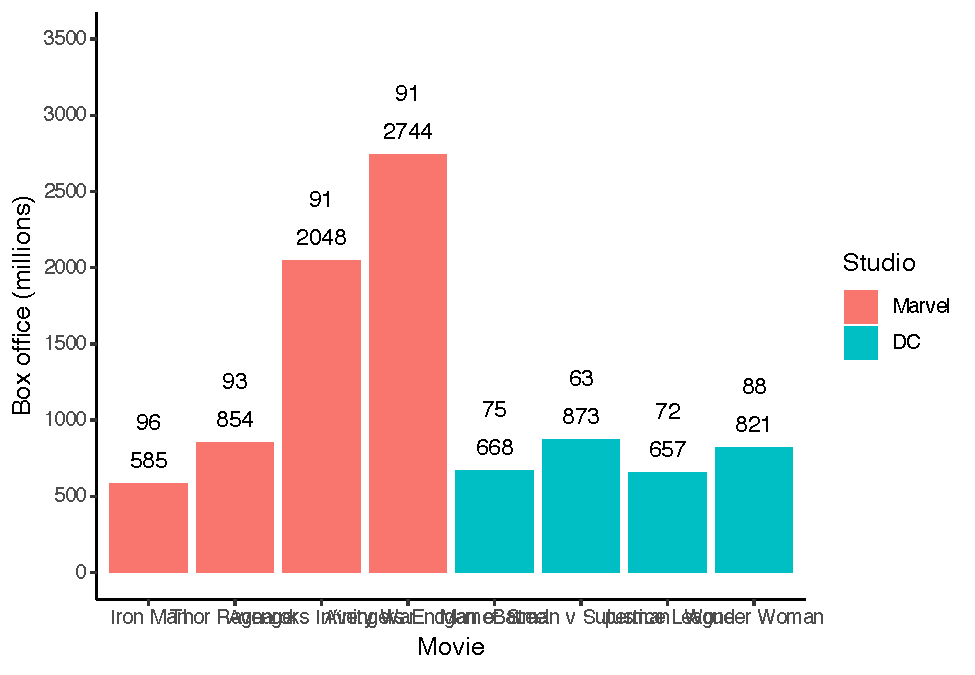
\includegraphics[width=0.65\linewidth]{bookdown_files/figure-latex/unnamed-chunk-125-1}

\hypertarget{order}{%
\subsection{Order}\label{order}}

\hypertarget{increasing-order}{%
\subsubsection{Increasing order}\label{increasing-order}}

We can make the movie bars go left to right in lowest to highest box office receipt order by changing the factor order prior to creating the graph. We do so with the mutate() and fct\_reorder() commands. The default order is ascending values even though we don't specify it.

\begin{Shaded}
\begin{Highlighting}[]
\NormalTok{movie_data <-}\StringTok{ }\NormalTok{movie_data }\OperatorTok\StringTok{ }
\StringTok{  }\KeywordTok{mutate}\NormalTok{(}\DataTypeTok{title =} \KeywordTok{fct_reorder}\NormalTok{(title,}
\NormalTok{                             boxoffice))}
\end{Highlighting}
\end{Shaded}

\begin{Shaded}
\begin{Highlighting}[]
\NormalTok{my_graph <-}\StringTok{ }\KeywordTok{ggplot}\NormalTok{(}\DataTypeTok{data =}\NormalTok{ movie_data,}
           \DataTypeTok{mapping =} \KeywordTok{aes}\NormalTok{(}\DataTypeTok{x =}\NormalTok{ title,}
                         \DataTypeTok{y =}\NormalTok{ boxoffice,}
                         \DataTypeTok{label =}\NormalTok{ boxoffice, }
                         \DataTypeTok{fill =}\NormalTok{ studio)) }\OperatorTok{+}
\StringTok{  }\KeywordTok{geom_col}\NormalTok{() }\OperatorTok{+}
\StringTok{  }\KeywordTok{geom_text}\NormalTok{(}\DataTypeTok{nudge_y =} \DecValTok{150}\NormalTok{)  }\OperatorTok{+}
\StringTok{  }\KeywordTok{geom_text}\NormalTok{(}\DataTypeTok{mapping =} \KeywordTok{aes}\NormalTok{(}\DataTypeTok{label =}\NormalTok{ tomatoes_aud), }
            \DataTypeTok{nudge_y =} \DecValTok{400}\NormalTok{) }\OperatorTok{+}
\StringTok{  }\KeywordTok{coord_cartesian}\NormalTok{(}\DataTypeTok{ylim =} \KeywordTok{c}\NormalTok{(}\DecValTok{0}\NormalTok{, }\DecValTok{3500}\NormalTok{)) }\OperatorTok{+}
\StringTok{  }\KeywordTok{scale_y_continuous}\NormalTok{(}\DataTypeTok{breaks =} \KeywordTok{seq}\NormalTok{(}\DecValTok{0}\NormalTok{, }\DecValTok{3500}\NormalTok{, }\DataTypeTok{by =} \DecValTok{500}\NormalTok{)) }\OperatorTok{+}
\StringTok{  }\KeywordTok{labs}\NormalTok{(}\DataTypeTok{x =} \StringTok{"Movie"}\NormalTok{,}
       \DataTypeTok{y =} \StringTok{"Box office (millions)"}\NormalTok{,}
       \DataTypeTok{fill =} \StringTok{"Studio"}\NormalTok{) }\OperatorTok{+}
\StringTok{  }\KeywordTok{theme_classic}\NormalTok{(}\DecValTok{12}\NormalTok{) }\OperatorTok{+}
\StringTok{  }\KeywordTok{theme}\NormalTok{(}\DataTypeTok{axis.text.x =} \KeywordTok{element_text}\NormalTok{(}\DataTypeTok{angle =} \DecValTok{60}\NormalTok{, }
                                   \DataTypeTok{hjust =} \DecValTok{1}\NormalTok{))  }

\KeywordTok{print}\NormalTok{(my_graph)}
\end{Highlighting}
\end{Shaded}

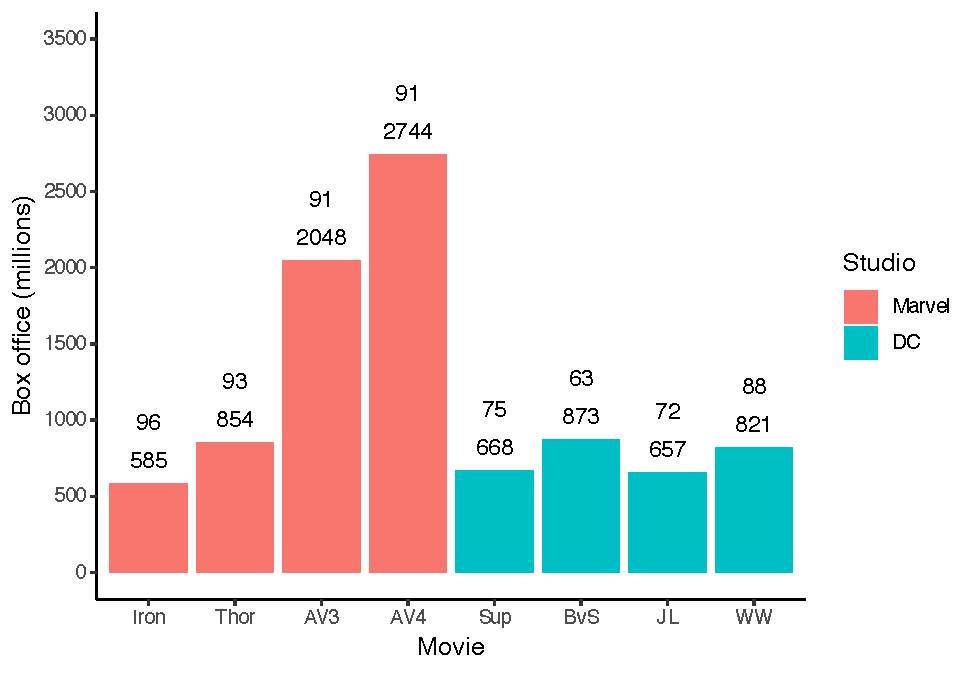
\includegraphics[width=0.65\linewidth]{bookdown_files/figure-latex/unnamed-chunk-127-1}

\hypertarget{decreasing-order}{%
\subsubsection{Decreasing order}\label{decreasing-order}}

We can make the movie bars go left to right in highest to lowest box office receipt order by changing the factor order prior to creating the graph. We use the same code as before but add the desc() command (i.e.,descending) around boxoffice in the fct\_reorder() call:

\begin{Shaded}
\begin{Highlighting}[]
\NormalTok{movie_data <-}\StringTok{ }\NormalTok{movie_data }\OperatorTok\StringTok{ }\KeywordTok{mutate}\NormalTok{(}\DataTypeTok{title =} \KeywordTok{fct_reorder}\NormalTok{(title,}
                                  \KeywordTok{desc}\NormalTok{(boxoffice)))}
\end{Highlighting}
\end{Shaded}

\begin{Shaded}
\begin{Highlighting}[]
\NormalTok{my_graph <-}\StringTok{ }\KeywordTok{ggplot}\NormalTok{(}\DataTypeTok{data =}\NormalTok{ movie_data,}
           \DataTypeTok{mapping =} \KeywordTok{aes}\NormalTok{(}\DataTypeTok{x =}\NormalTok{ title,}
                         \DataTypeTok{y =}\NormalTok{ boxoffice,}
                         \DataTypeTok{label =}\NormalTok{ boxoffice, }
                         \DataTypeTok{fill =}\NormalTok{ studio)) }\OperatorTok{+}
\StringTok{  }\KeywordTok{geom_col}\NormalTok{() }\OperatorTok{+}
\StringTok{  }\KeywordTok{geom_text}\NormalTok{(}\DataTypeTok{nudge_y =} \DecValTok{150}\NormalTok{)  }\OperatorTok{+}
\StringTok{  }\KeywordTok{geom_text}\NormalTok{(}\DataTypeTok{mapping =} \KeywordTok{aes}\NormalTok{(}\DataTypeTok{label =}\NormalTok{ tomatoes_aud), }
            \DataTypeTok{nudge_y =} \DecValTok{400}\NormalTok{) }\OperatorTok{+}
\StringTok{  }\KeywordTok{coord_cartesian}\NormalTok{(}\DataTypeTok{ylim =} \KeywordTok{c}\NormalTok{(}\DecValTok{0}\NormalTok{, }\DecValTok{3500}\NormalTok{)) }\OperatorTok{+}
\StringTok{  }\KeywordTok{scale_y_continuous}\NormalTok{(}\DataTypeTok{breaks =} \KeywordTok{seq}\NormalTok{(}\DecValTok{0}\NormalTok{, }\DecValTok{3500}\NormalTok{, }\DataTypeTok{by =} \DecValTok{500}\NormalTok{)) }\OperatorTok{+}
\StringTok{  }\KeywordTok{labs}\NormalTok{(}\DataTypeTok{x =} \StringTok{"Movie"}\NormalTok{,}
       \DataTypeTok{y =} \StringTok{"Box office (millions)"}\NormalTok{,}
       \DataTypeTok{fill =} \StringTok{"Studio"}\NormalTok{) }\OperatorTok{+}
\StringTok{  }\KeywordTok{theme_classic}\NormalTok{(}\DecValTok{12}\NormalTok{) }\OperatorTok{+}
\StringTok{  }\KeywordTok{theme}\NormalTok{(}\DataTypeTok{axis.text.x =} \KeywordTok{element_text}\NormalTok{(}\DataTypeTok{angle =} \DecValTok{60}\NormalTok{, }
                                   \DataTypeTok{hjust =} \DecValTok{1}\NormalTok{))  }

\KeywordTok{print}\NormalTok{(my_graph)}
\end{Highlighting}
\end{Shaded}

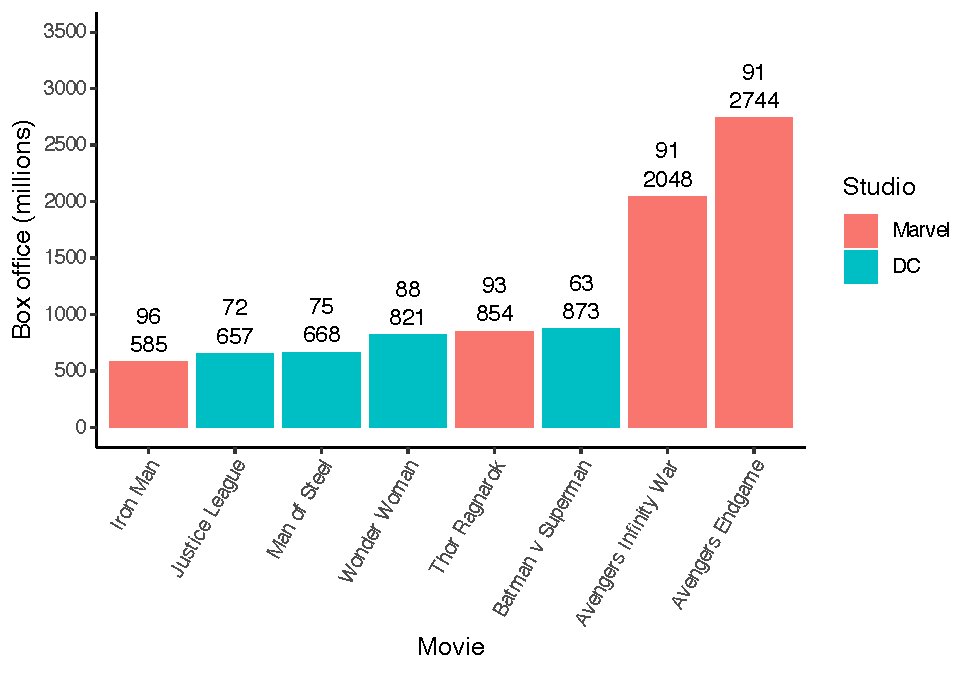
\includegraphics[width=0.65\linewidth]{bookdown_files/figure-latex/unnamed-chunk-129-1}

\hypertarget{custom-order}{%
\subsubsection{Custom order}\label{custom-order}}

We can make the movie bars go left to right in a custom order by changing the factor order prior to creating the graph. Because we want a custom order of the factor levels we use fct\_relevel(), instead of the the fct\_reorder() command from the previous two examples. Below I use this approach to manually order movies highest to lowest boxoffice within movie studio (Marvel or DC).

\begin{Shaded}
\begin{Highlighting}[]
\NormalTok{movie_data <-}\StringTok{ }\NormalTok{movie_data }\OperatorTok\StringTok{ }
\StringTok{  }\KeywordTok{mutate}\NormalTok{(}\DataTypeTok{title =} \KeywordTok{fct_relevel}\NormalTok{(title,}
                             \StringTok{"Avengers Endgame"}\NormalTok{,}
                             \StringTok{"Avengers Infinity War"}\NormalTok{,}
                             \StringTok{"Thor Ragnarok"}\NormalTok{,}
                             \StringTok{"Iron Man"}\NormalTok{,}
                             \StringTok{"Batman v Superman"}\NormalTok{,}
                             \StringTok{"Wonder Woman"}\NormalTok{,}
                             \StringTok{"Man of Steel"}\NormalTok{,}
                             \StringTok{"Justice League"}\NormalTok{))}
\end{Highlighting}
\end{Shaded}

\begin{Shaded}
\begin{Highlighting}[]
\NormalTok{my_graph <-}\StringTok{ }\KeywordTok{ggplot}\NormalTok{(}\DataTypeTok{data =}\NormalTok{ movie_data,}
           \DataTypeTok{mapping =} \KeywordTok{aes}\NormalTok{(}\DataTypeTok{x =}\NormalTok{ title,}
                         \DataTypeTok{y =}\NormalTok{ boxoffice,}
                         \DataTypeTok{label =}\NormalTok{ boxoffice, }
                         \DataTypeTok{fill =}\NormalTok{ studio)) }\OperatorTok{+}
\StringTok{  }\KeywordTok{geom_col}\NormalTok{() }\OperatorTok{+}
\StringTok{  }\KeywordTok{geom_text}\NormalTok{(}\DataTypeTok{nudge_y =} \DecValTok{150}\NormalTok{)  }\OperatorTok{+}
\StringTok{  }\KeywordTok{geom_text}\NormalTok{(}\DataTypeTok{mapping =} \KeywordTok{aes}\NormalTok{(}\DataTypeTok{label =}\NormalTok{ tomatoes_aud), }
            \DataTypeTok{nudge_y =} \DecValTok{400}\NormalTok{) }\OperatorTok{+}
\StringTok{  }\KeywordTok{coord_cartesian}\NormalTok{(}\DataTypeTok{ylim =} \KeywordTok{c}\NormalTok{(}\DecValTok{0}\NormalTok{, }\DecValTok{3500}\NormalTok{)) }\OperatorTok{+}
\StringTok{  }\KeywordTok{scale_y_continuous}\NormalTok{(}\DataTypeTok{breaks =} \KeywordTok{seq}\NormalTok{(}\DecValTok{0}\NormalTok{, }\DecValTok{3500}\NormalTok{, }\DataTypeTok{by =} \DecValTok{500}\NormalTok{)) }\OperatorTok{+}
\StringTok{  }\KeywordTok{labs}\NormalTok{(}\DataTypeTok{x =} \StringTok{"Movie"}\NormalTok{,}
       \DataTypeTok{y =} \StringTok{"Box office (millions)"}\NormalTok{,}
       \DataTypeTok{fill =} \StringTok{"Studio"}\NormalTok{) }\OperatorTok{+}
\StringTok{  }\KeywordTok{theme_classic}\NormalTok{(}\DecValTok{12}\NormalTok{) }\OperatorTok{+}
\StringTok{  }\KeywordTok{theme}\NormalTok{(}\DataTypeTok{axis.text.x =} \KeywordTok{element_text}\NormalTok{(}\DataTypeTok{angle =} \DecValTok{60}\NormalTok{, }
                                   \DataTypeTok{hjust =} \DecValTok{1}\NormalTok{))  }
\end{Highlighting}
\end{Shaded}

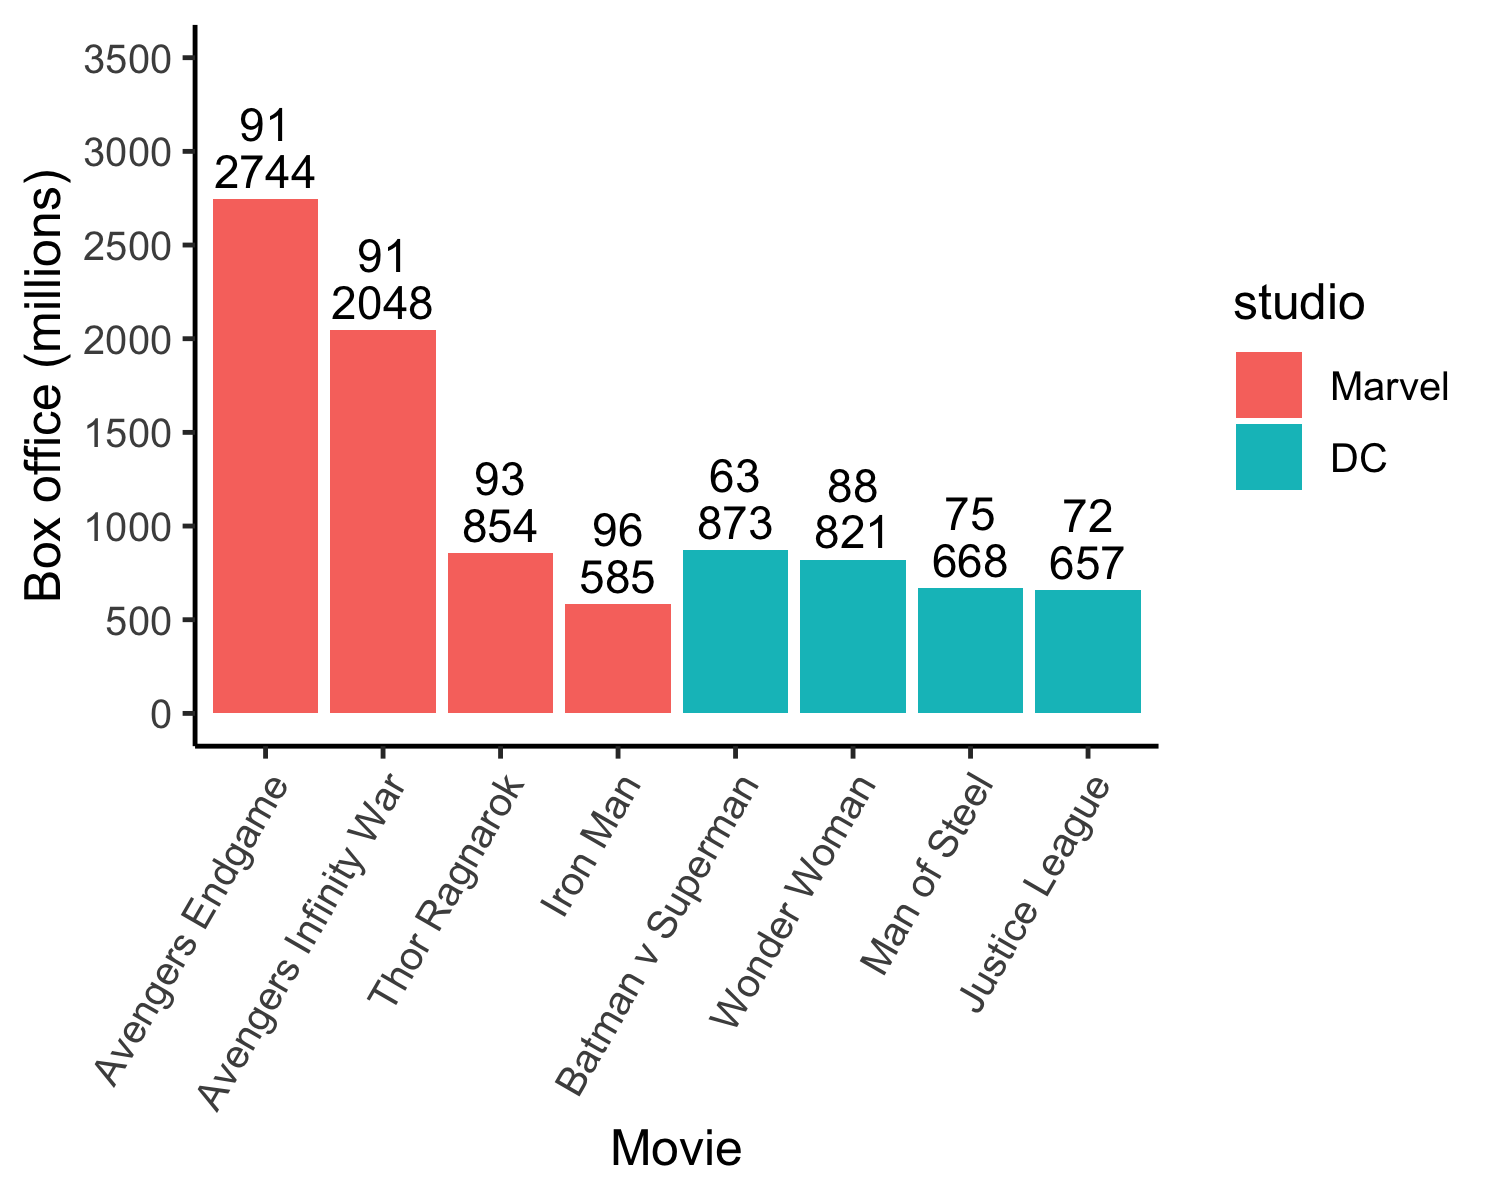
\includegraphics[width=0.65\linewidth]{ch_graphing/images/custom_order}

\hypertarget{legend-order}{%
\subsection{Legend order}\label{legend-order}}

After inspecting the graph on the previous page, you might think that Marvel should be above DC in the legend. You can do that by reordering the studio factor:

\begin{Shaded}
\begin{Highlighting}[]
\NormalTok{movie_data <-}\StringTok{ }\NormalTok{movie_data }\OperatorTok\StringTok{ }
\StringTok{  }\KeywordTok{mutate}\NormalTok{(}\DataTypeTok{studio =} \KeywordTok{fct_relevel}\NormalTok{(studio,}
                             \StringTok{"Marvel"}\NormalTok{,}
                             \StringTok{"DC"}\NormalTok{))}
\end{Highlighting}
\end{Shaded}

\begin{Shaded}
\begin{Highlighting}[]
\NormalTok{my_graph <-}\StringTok{ }\KeywordTok{ggplot}\NormalTok{(}\DataTypeTok{data =}\NormalTok{ movie_data,}
           \DataTypeTok{mapping =} \KeywordTok{aes}\NormalTok{(}\DataTypeTok{x =}\NormalTok{ title,}
                         \DataTypeTok{y =}\NormalTok{ boxoffice,}
                         \DataTypeTok{label =}\NormalTok{ boxoffice, }
                         \DataTypeTok{fill =}\NormalTok{ studio)) }\OperatorTok{+}
\StringTok{  }\KeywordTok{geom_col}\NormalTok{() }\OperatorTok{+}
\StringTok{  }\KeywordTok{geom_text}\NormalTok{(}\DataTypeTok{nudge_y =} \DecValTok{150}\NormalTok{)  }\OperatorTok{+}
\StringTok{  }\KeywordTok{geom_text}\NormalTok{(}\DataTypeTok{mapping =} \KeywordTok{aes}\NormalTok{(}\DataTypeTok{label =}\NormalTok{ tomatoes_aud), }
            \DataTypeTok{nudge_y =} \DecValTok{400}\NormalTok{) }\OperatorTok{+}
\StringTok{  }\KeywordTok{coord_cartesian}\NormalTok{(}\DataTypeTok{ylim =} \KeywordTok{c}\NormalTok{(}\DecValTok{0}\NormalTok{, }\DecValTok{3500}\NormalTok{)) }\OperatorTok{+}
\StringTok{  }\KeywordTok{scale_y_continuous}\NormalTok{(}\DataTypeTok{breaks =} \KeywordTok{seq}\NormalTok{(}\DecValTok{0}\NormalTok{, }\DecValTok{3500}\NormalTok{, }\DataTypeTok{by =} \DecValTok{500}\NormalTok{)) }\OperatorTok{+}
\StringTok{  }\KeywordTok{labs}\NormalTok{(}\DataTypeTok{x =} \StringTok{"Movie"}\NormalTok{,}
       \DataTypeTok{y =} \StringTok{"Box office (millions)"}\NormalTok{,}
       \DataTypeTok{fill =} \StringTok{"Studio"}\NormalTok{) }\OperatorTok{+}
\StringTok{  }\KeywordTok{theme_classic}\NormalTok{(}\DecValTok{12}\NormalTok{) }\OperatorTok{+}
\StringTok{  }\KeywordTok{theme}\NormalTok{(}\DataTypeTok{axis.text.x =} \KeywordTok{element_text}\NormalTok{(}\DataTypeTok{angle =} \DecValTok{60}\NormalTok{, }
                                   \DataTypeTok{hjust =} \DecValTok{1}\NormalTok{))  }
\end{Highlighting}
\end{Shaded}

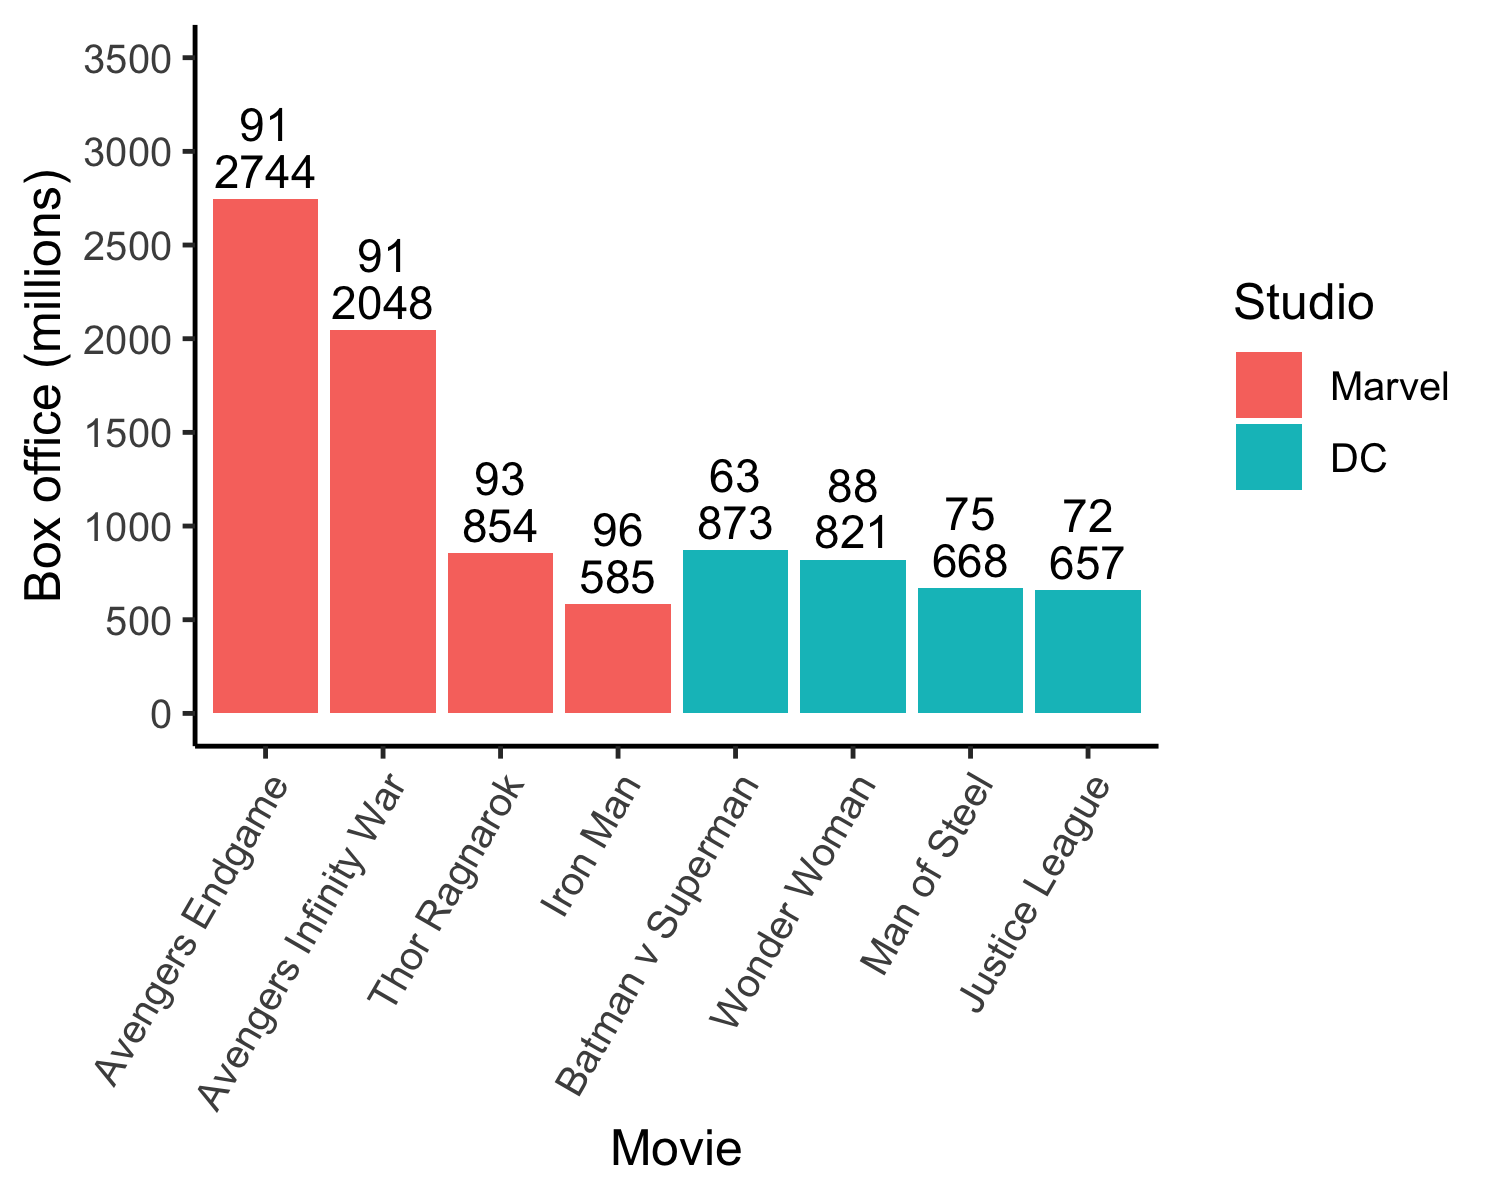
\includegraphics[width=0.65\linewidth]{ch_graphing/images/custom_order2}

\hypertarget{custom-colours}{%
\section{Custom colours}\label{custom-colours}}

\hypertarget{r-palette}{%
\subsection{R palette}\label{r-palette}}

You might look at the previous graph and think ``Marvel should be red and DC should be blue since those are the colours of their respective logos''. You can do that with the code below. Note that you specify the colours in the order the names appear in the legend (top to bottom).

R colour names/pictures can be found here: \url{http://sape.inf.usi.ch/quick-reference/ggplot2/colour}

\begin{Shaded}
\begin{Highlighting}[]
\NormalTok{my_graph <-}\StringTok{ }\KeywordTok{ggplot}\NormalTok{(}\DataTypeTok{data =}\NormalTok{ movie_data,}
           \DataTypeTok{mapping =} \KeywordTok{aes}\NormalTok{(}\DataTypeTok{x =}\NormalTok{ title,}
                         \DataTypeTok{y =}\NormalTok{ boxoffice,}
                         \DataTypeTok{label =}\NormalTok{ boxoffice, }
                         \DataTypeTok{fill =}\NormalTok{ studio)) }\OperatorTok{+}
\StringTok{  }\KeywordTok{geom_col}\NormalTok{() }\OperatorTok{+}
\StringTok{  }\KeywordTok{geom_text}\NormalTok{(}\DataTypeTok{nudge_y =} \DecValTok{150}\NormalTok{)  }\OperatorTok{+}
\StringTok{  }\KeywordTok{geom_text}\NormalTok{(}\DataTypeTok{mapping =} \KeywordTok{aes}\NormalTok{(}\DataTypeTok{label =}\NormalTok{ tomatoes_aud), }
            \DataTypeTok{nudge_y =} \DecValTok{400}\NormalTok{) }\OperatorTok{+}
\StringTok{  }\KeywordTok{coord_cartesian}\NormalTok{(}\DataTypeTok{ylim =} \KeywordTok{c}\NormalTok{(}\DecValTok{0}\NormalTok{, }\DecValTok{3500}\NormalTok{)) }\OperatorTok{+}
\StringTok{  }\KeywordTok{scale_y_continuous}\NormalTok{(}\DataTypeTok{breaks =} \KeywordTok{seq}\NormalTok{(}\DecValTok{0}\NormalTok{, }\DecValTok{3500}\NormalTok{, }\DataTypeTok{by =} \DecValTok{500}\NormalTok{)) }\OperatorTok{+}
\StringTok{  }\KeywordTok{labs}\NormalTok{(}\DataTypeTok{x =} \StringTok{"Movie"}\NormalTok{,}
       \DataTypeTok{y =} \StringTok{"Box office (millions)"}\NormalTok{,}
       \DataTypeTok{fill =} \StringTok{"Studio"}\NormalTok{) }\OperatorTok{+}
\StringTok{  }\KeywordTok{theme_classic}\NormalTok{(}\DecValTok{12}\NormalTok{) }\OperatorTok{+}
\StringTok{  }\KeywordTok{theme}\NormalTok{(}\DataTypeTok{axis.text.x =} \KeywordTok{element_text}\NormalTok{(}\DataTypeTok{angle =} \DecValTok{60}\NormalTok{, }
                                   \DataTypeTok{hjust =} \DecValTok{1}\NormalTok{)) }\OperatorTok{+}
\StringTok{  }\KeywordTok{scale_fill_manual}\NormalTok{(}\DataTypeTok{values =} \KeywordTok{c}\NormalTok{(}\StringTok{"red"}\NormalTok{, }\StringTok{"blue"}\NormalTok{))}
\end{Highlighting}
\end{Shaded}

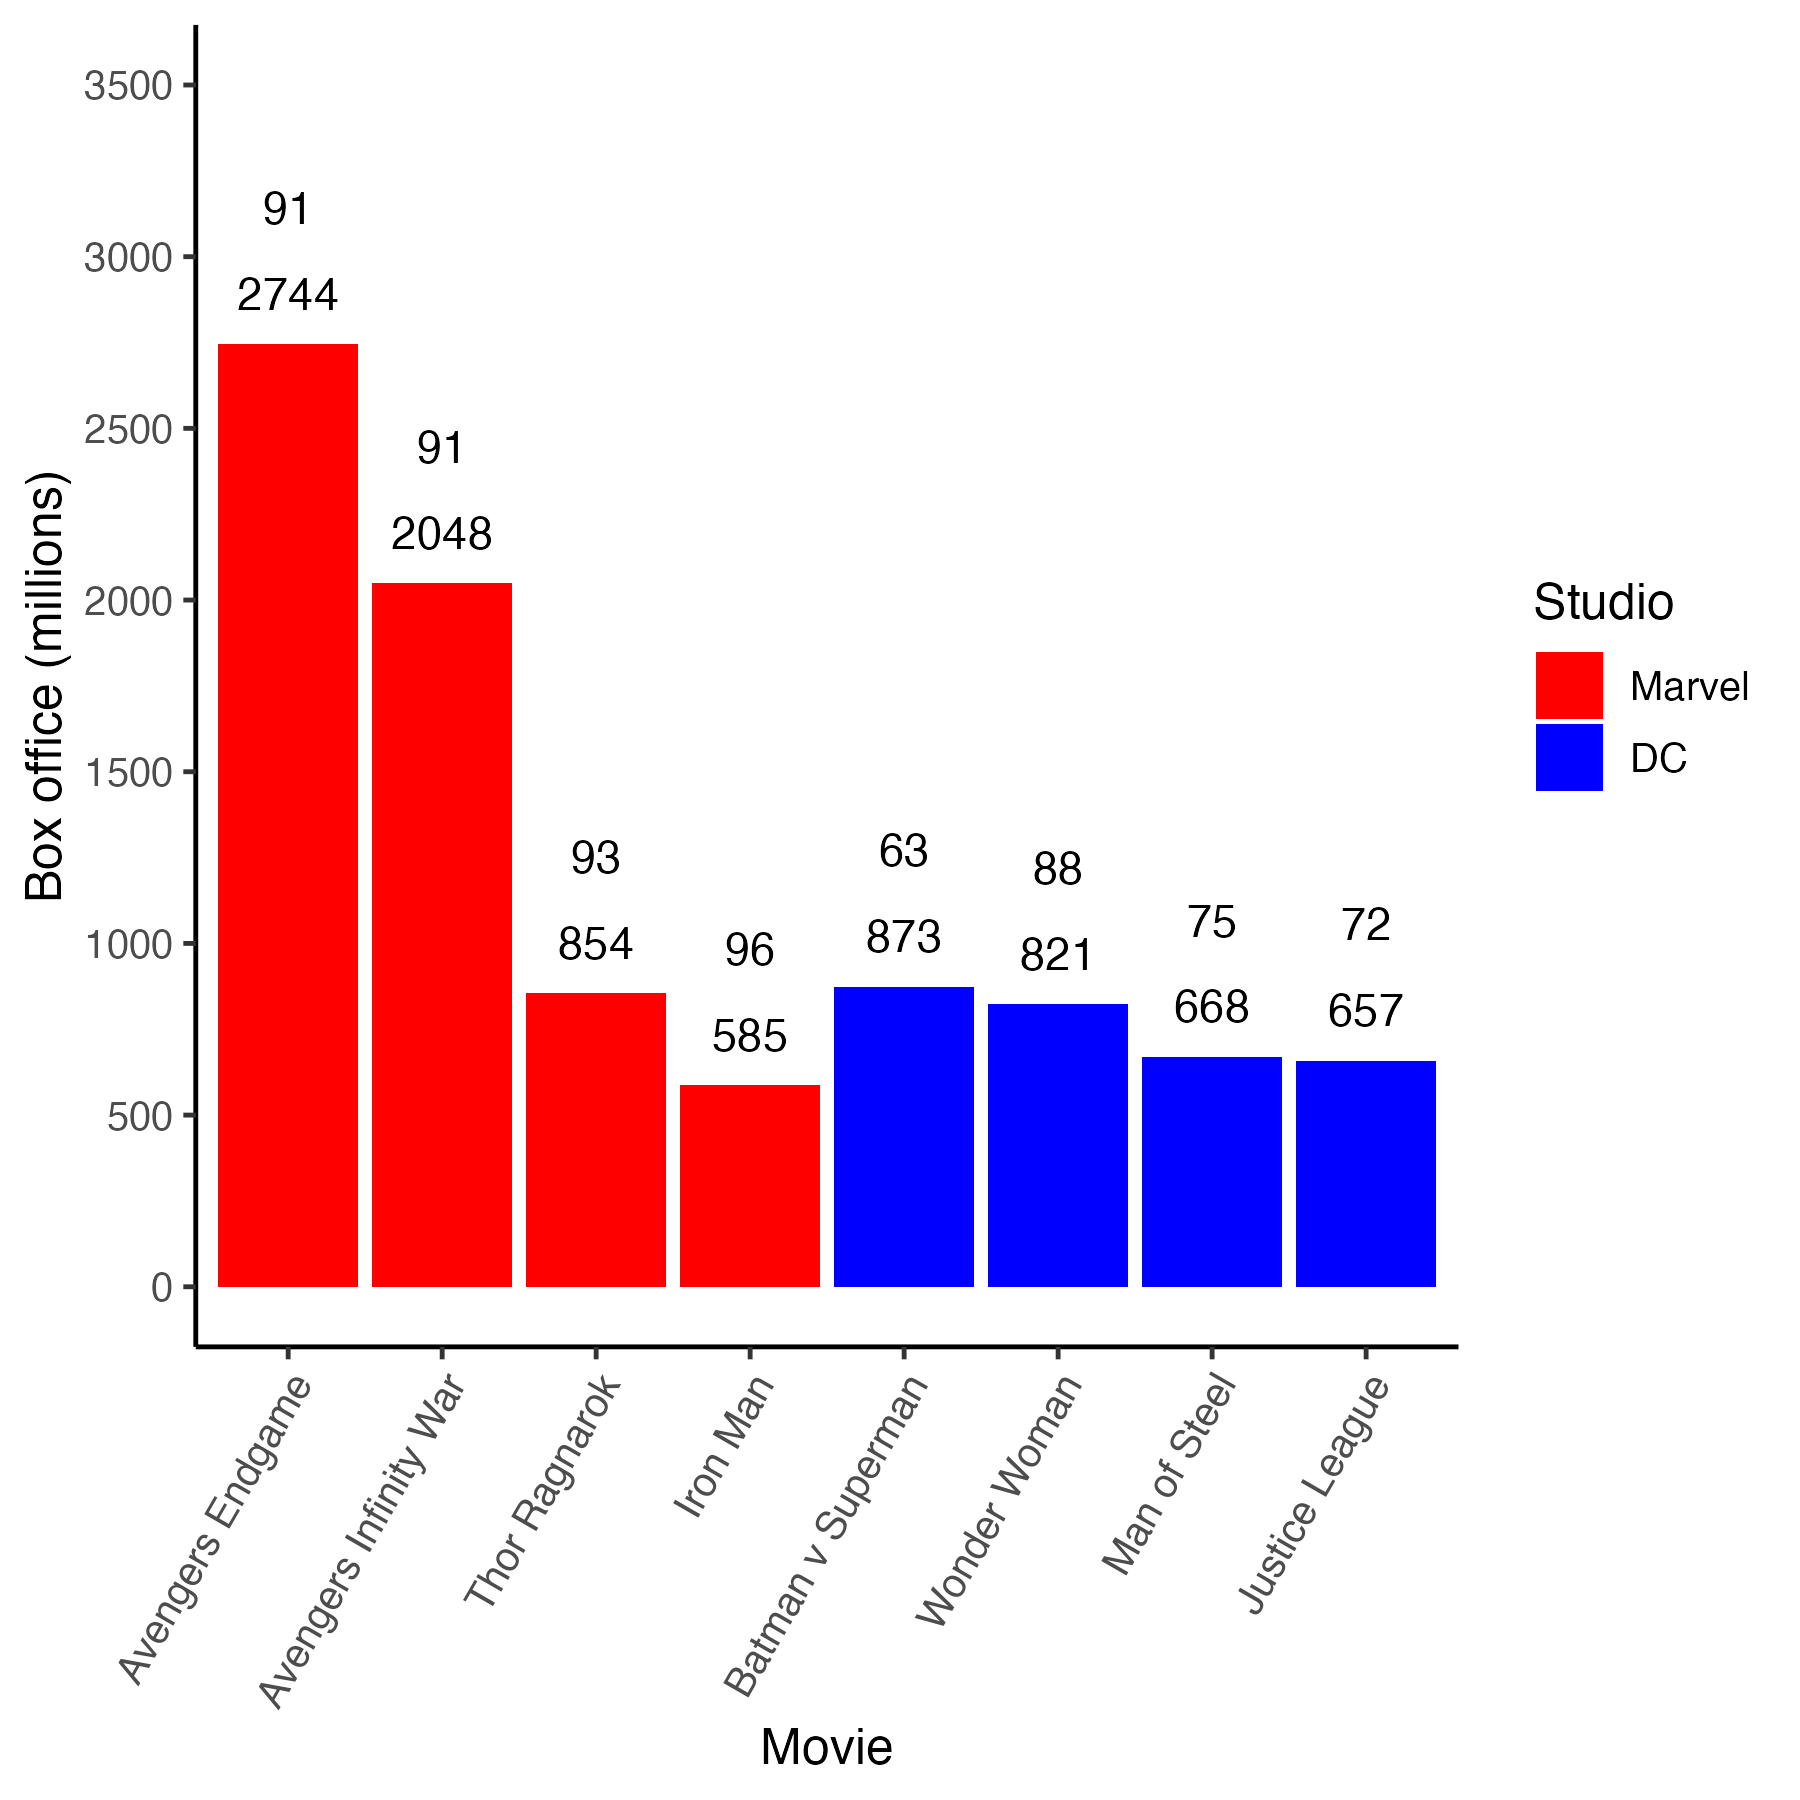
\includegraphics[width=0.65\linewidth]{ch_graphing/images/base_color_graph}

\hypertarget{hex-colours}{%
\subsection{Hex colours}\label{hex-colours}}

If you are a really big geek (like me) you might look at the previous graph and think ``Those aren't the proper colours for the Marvel and DC - lame!'' So\ldots{} you do some internet research and determine that you can specify colours using hexidecimal numbers. More specifically, you find Marvel red is \#ed1d24 and DC blue is \#0476F2 using hex colour codes. You can use those precise colours via the scale\_fill\_manual() command below.

\begin{Shaded}
\begin{Highlighting}[]
\NormalTok{my_graph <-}\StringTok{ }\KeywordTok{ggplot}\NormalTok{(}\DataTypeTok{data =}\NormalTok{ movie_data,}
           \DataTypeTok{mapping =} \KeywordTok{aes}\NormalTok{(}\DataTypeTok{x =}\NormalTok{ title,}
                         \DataTypeTok{y =}\NormalTok{ boxoffice,}
                         \DataTypeTok{label =}\NormalTok{ boxoffice, }
                         \DataTypeTok{fill =}\NormalTok{ studio)) }\OperatorTok{+}
\StringTok{  }\KeywordTok{geom_col}\NormalTok{() }\OperatorTok{+}
\StringTok{  }\KeywordTok{geom_text}\NormalTok{(}\DataTypeTok{nudge_y =} \DecValTok{150}\NormalTok{)  }\OperatorTok{+}
\StringTok{  }\KeywordTok{geom_text}\NormalTok{(}\DataTypeTok{mapping =} \KeywordTok{aes}\NormalTok{(}\DataTypeTok{label =}\NormalTok{ tomatoes_aud), }
            \DataTypeTok{nudge_y =} \DecValTok{400}\NormalTok{) }\OperatorTok{+}
\StringTok{  }\KeywordTok{coord_cartesian}\NormalTok{(}\DataTypeTok{ylim =} \KeywordTok{c}\NormalTok{(}\DecValTok{0}\NormalTok{, }\DecValTok{3500}\NormalTok{)) }\OperatorTok{+}
\StringTok{  }\KeywordTok{scale_y_continuous}\NormalTok{(}\DataTypeTok{breaks =} \KeywordTok{seq}\NormalTok{(}\DecValTok{0}\NormalTok{, }\DecValTok{3500}\NormalTok{, }\DataTypeTok{by =} \DecValTok{500}\NormalTok{)) }\OperatorTok{+}
\StringTok{  }\KeywordTok{labs}\NormalTok{(}\DataTypeTok{x =} \StringTok{"Movie"}\NormalTok{,}
       \DataTypeTok{y =} \StringTok{"Box office (millions)"}\NormalTok{,}
       \DataTypeTok{fill =} \StringTok{"Studio"}\NormalTok{) }\OperatorTok{+}
\StringTok{  }\KeywordTok{theme_classic}\NormalTok{(}\DecValTok{12}\NormalTok{) }\OperatorTok{+}
\StringTok{  }\KeywordTok{theme}\NormalTok{(}\DataTypeTok{axis.text.x =} \KeywordTok{element_text}\NormalTok{(}\DataTypeTok{angle =} \DecValTok{60}\NormalTok{, }
                                   \DataTypeTok{hjust =} \DecValTok{1}\NormalTok{)) }\OperatorTok{+}
\StringTok{  }\KeywordTok{scale_fill_manual}\NormalTok{(}\DataTypeTok{values =} \KeywordTok{c}\NormalTok{(}\StringTok{"#ed1d24"}\NormalTok{, }\StringTok{"#0476F2"}\NormalTok{))}
\end{Highlighting}
\end{Shaded}

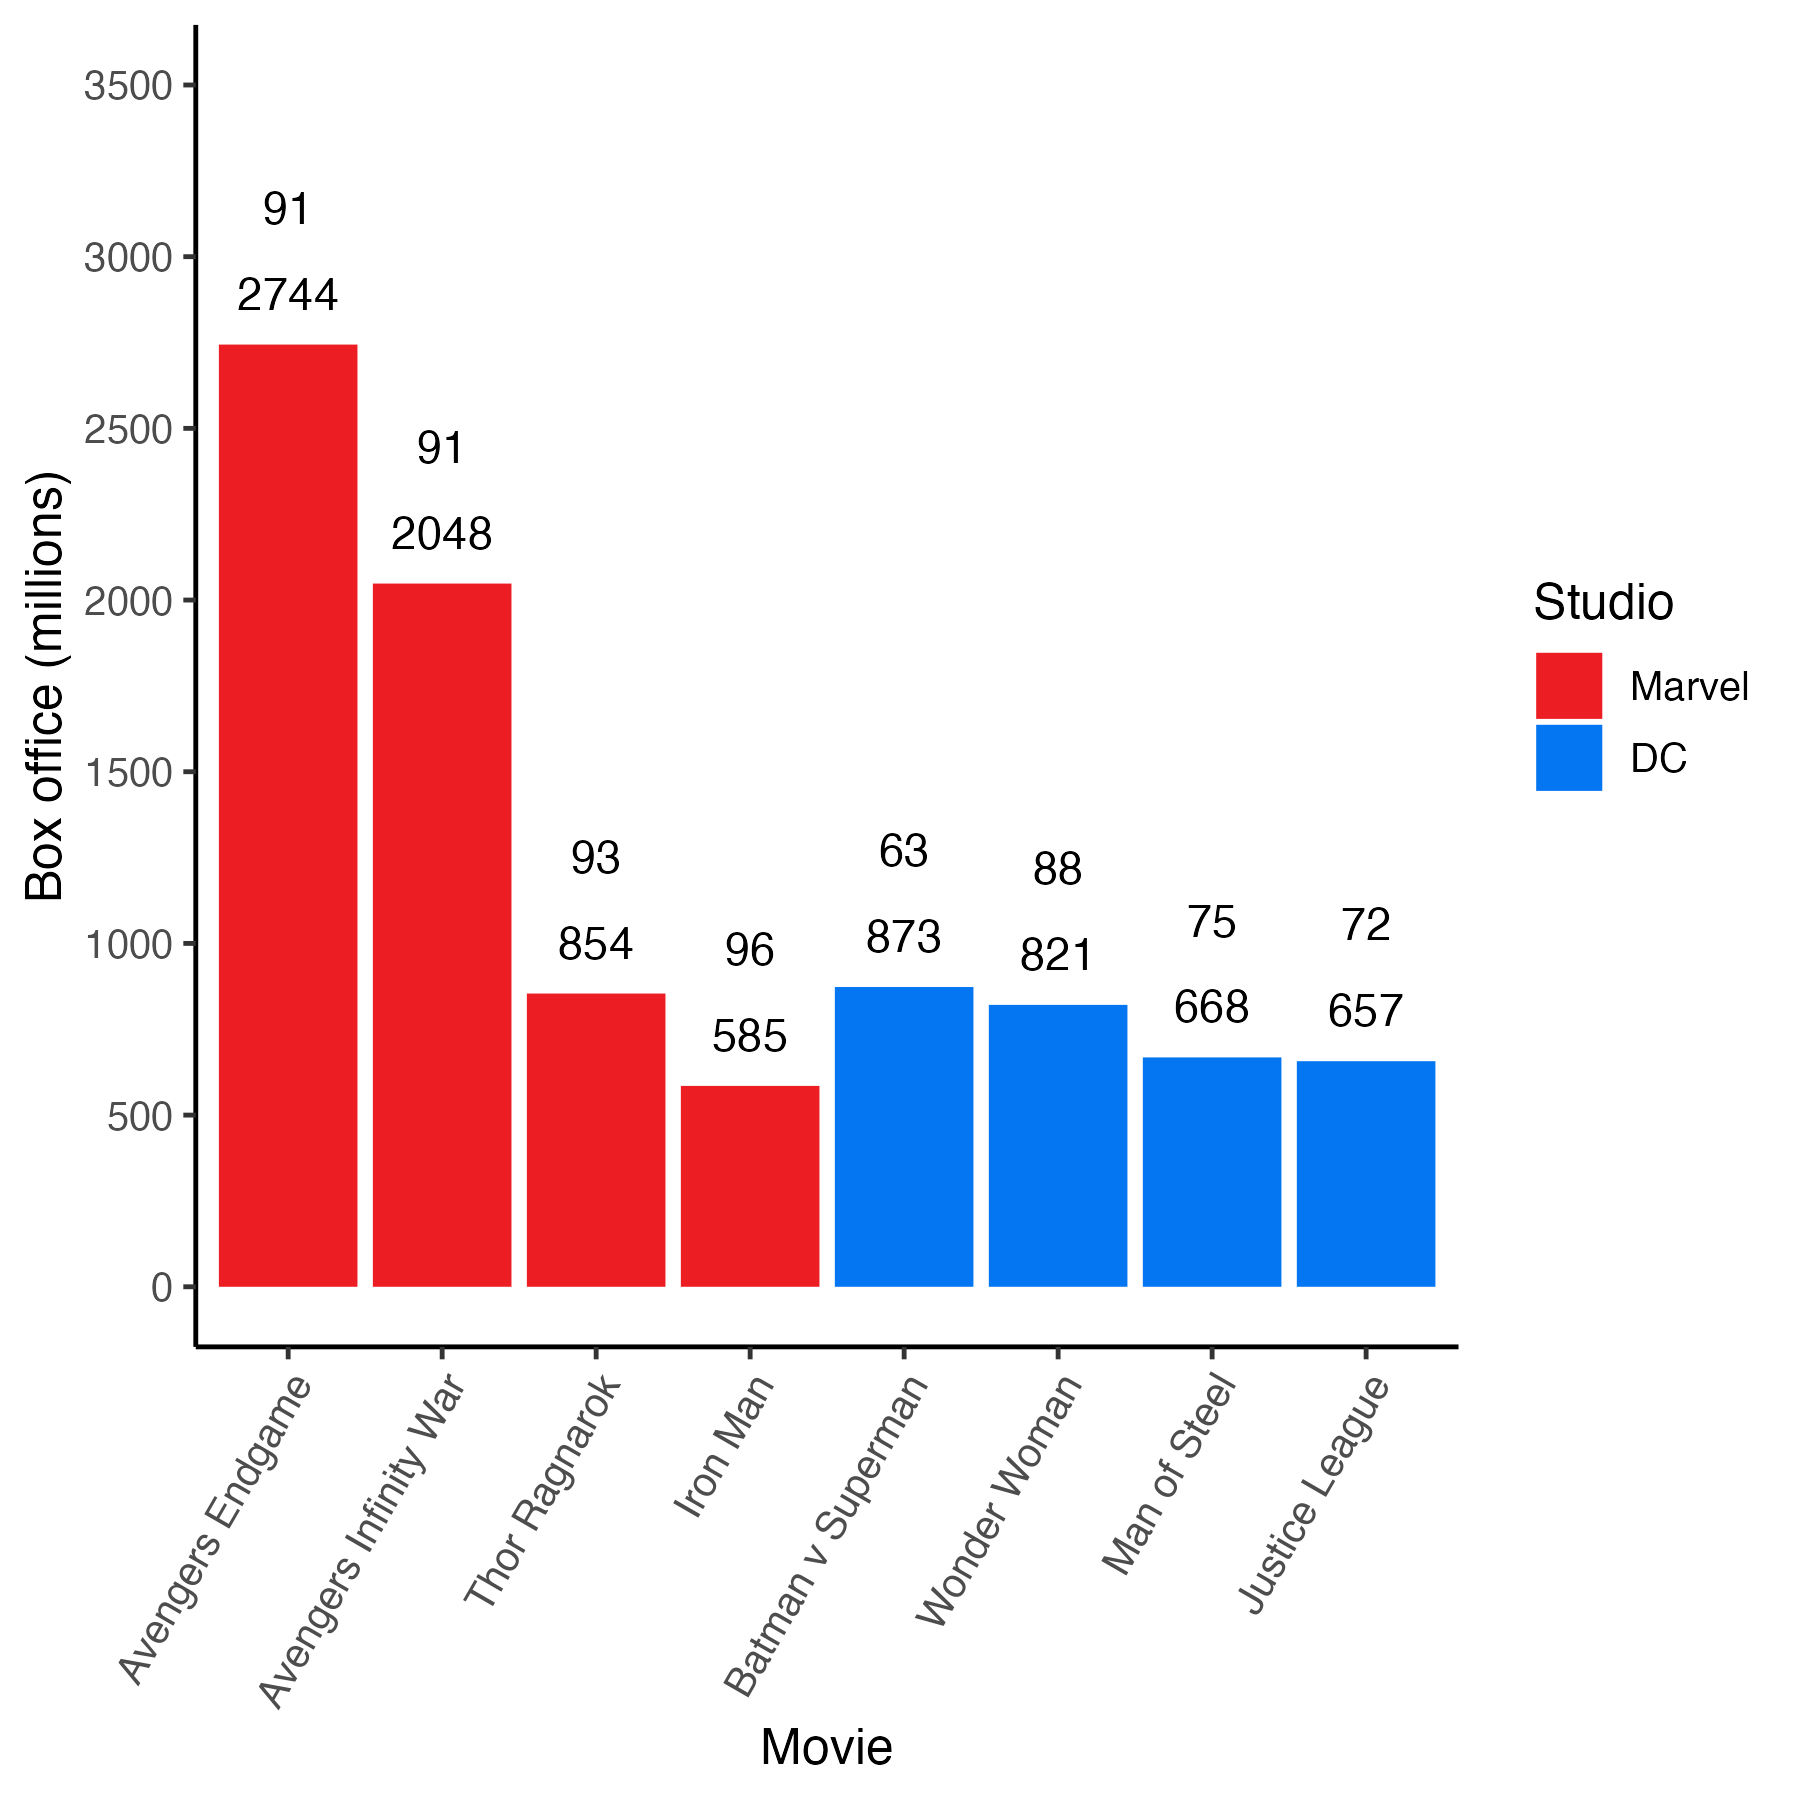
\includegraphics[width=0.65\linewidth]{ch_graphing/images/logo_color_graph}

\hypertarget{emoji}{%
\section{Emoji}\label{emoji}}

Make the graph more fun with the emoGG package. You might like to make the graph more fun by putting tomatoes on the graph to indicate what the extra numbers mean. We can do that with the emoGG package. The installation instructions for this package are at the start of this chapter; note, that it is installed via GitHub rather than the CRAN. Course R Studio Cloud users - the installation has already been done.

After installation you need to activate the emoGG package:

\begin{Shaded}
\begin{Highlighting}[]
\KeywordTok{library}\NormalTok{(emoGG)}
\end{Highlighting}
\end{Shaded}

Visit this link to check out the codes for emoji: \url{https://apps.timwhitlock.info/emoji/tables/unicode}

If you scroll down to section 5 Uncategorized on this page you will find the code for a tomato is 1f345. Note that the code below will only work with an internet connection. The command geom\_emoji() needs internet access to retrieve the emoji graphic requested.

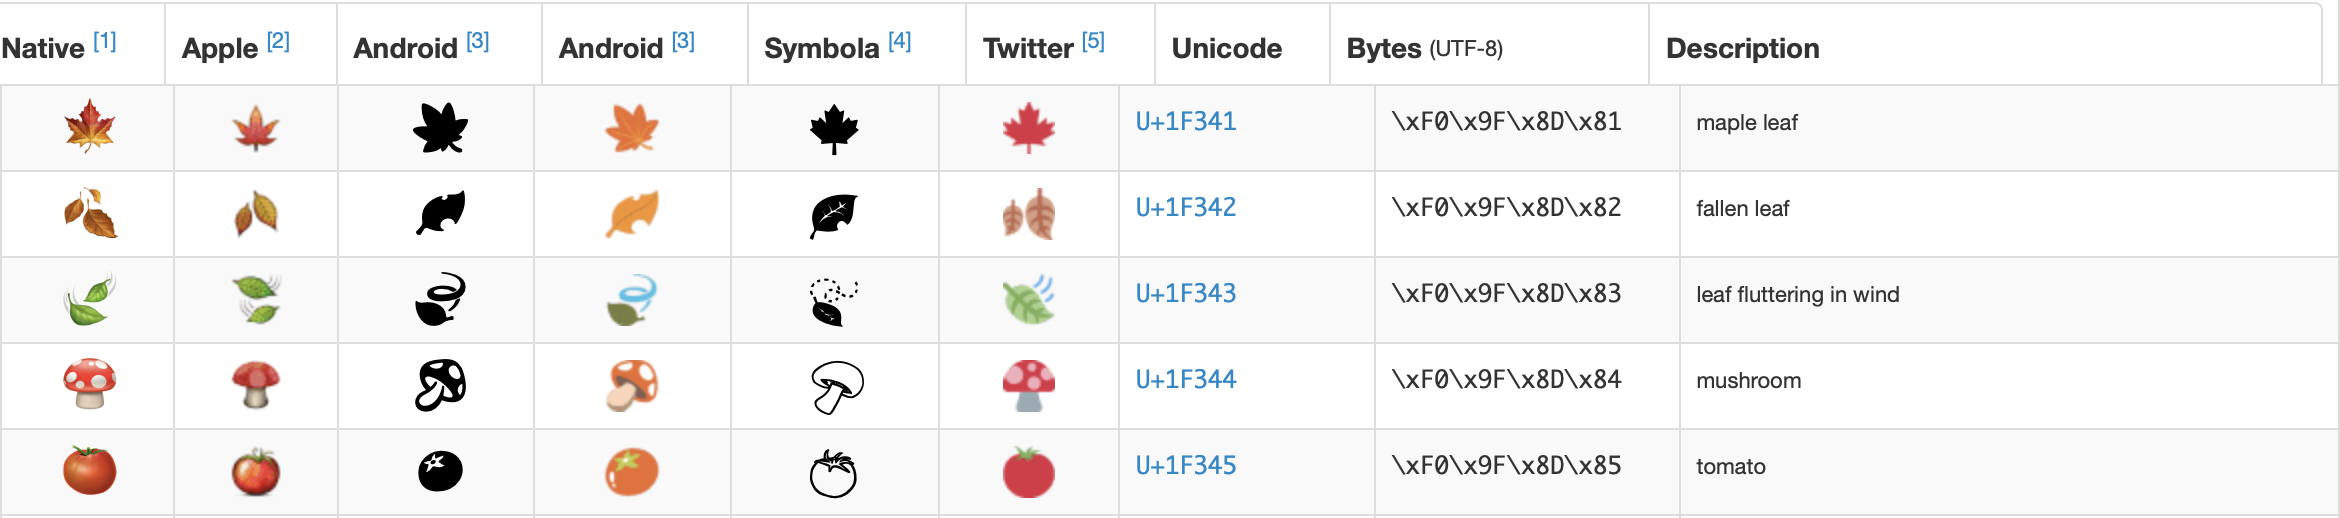
\includegraphics[width=0.9\linewidth]{ch_graphing/images/emoji_table}

\begin{Shaded}
\begin{Highlighting}[]
\NormalTok{my_graph <-}\StringTok{ }\KeywordTok{ggplot}\NormalTok{(}\DataTypeTok{data =}\NormalTok{ movie_data,}
           \DataTypeTok{mapping =} \KeywordTok{aes}\NormalTok{(}\DataTypeTok{x =}\NormalTok{ title,}
                         \DataTypeTok{y =}\NormalTok{ boxoffice,}
                         \DataTypeTok{label =}\NormalTok{ boxoffice, }
                         \DataTypeTok{fill =}\NormalTok{ studio)) }\OperatorTok{+}
\StringTok{  }\KeywordTok{geom_col}\NormalTok{() }\OperatorTok{+}
\StringTok{  }\KeywordTok{geom_text}\NormalTok{(}\DataTypeTok{nudge_y =} \DecValTok{150}\NormalTok{)  }\OperatorTok{+}
\StringTok{  }\KeywordTok{geom_text}\NormalTok{(}\DataTypeTok{mapping =} \KeywordTok{aes}\NormalTok{(}\DataTypeTok{label =}\NormalTok{ tomatoes_aud), }
            \DataTypeTok{nudge_y =} \DecValTok{600}\NormalTok{, }
            \DataTypeTok{colour =} \StringTok{"red"}\NormalTok{) }\OperatorTok{+}
\StringTok{  }\KeywordTok{geom_emoji}\NormalTok{(}\DataTypeTok{mapping =} \KeywordTok{aes}\NormalTok{(}\DataTypeTok{y =}\NormalTok{ boxoffice }\OperatorTok{+}\StringTok{ }\DecValTok{400}\NormalTok{),}
             \DataTypeTok{emoji=}\StringTok{"1f345"}\NormalTok{) }\OperatorTok{+}
\StringTok{  }\KeywordTok{coord_cartesian}\NormalTok{(}\DataTypeTok{ylim =} \KeywordTok{c}\NormalTok{(}\DecValTok{0}\NormalTok{, }\DecValTok{3500}\NormalTok{)) }\OperatorTok{+}
\StringTok{  }\KeywordTok{scale_y_continuous}\NormalTok{(}\DataTypeTok{breaks =} \KeywordTok{seq}\NormalTok{(}\DecValTok{0}\NormalTok{, }\DecValTok{3500}\NormalTok{, }\DataTypeTok{by =} \DecValTok{500}\NormalTok{)) }\OperatorTok{+}
\StringTok{  }\KeywordTok{labs}\NormalTok{(}\DataTypeTok{x =} \StringTok{"Movie"}\NormalTok{,}
       \DataTypeTok{y =} \StringTok{"Box office (millions)"}\NormalTok{,}
       \DataTypeTok{fill =} \StringTok{"Studio"}\NormalTok{) }\OperatorTok{+}
\StringTok{  }\KeywordTok{theme_classic}\NormalTok{(}\DecValTok{12}\NormalTok{) }\OperatorTok{+}
\StringTok{  }\KeywordTok{theme}\NormalTok{(}\DataTypeTok{axis.text.x =} \KeywordTok{element_text}\NormalTok{(}\DataTypeTok{angle =} \DecValTok{60}\NormalTok{, }
                                   \DataTypeTok{hjust =} \DecValTok{1}\NormalTok{)) }\OperatorTok{+}
\StringTok{  }\KeywordTok{scale_fill_manual}\NormalTok{(}\DataTypeTok{values =} \KeywordTok{c}\NormalTok{(}\StringTok{"#ed1d24"}\NormalTok{, }\StringTok{"#0476F2"}\NormalTok{))}
\end{Highlighting}
\end{Shaded}

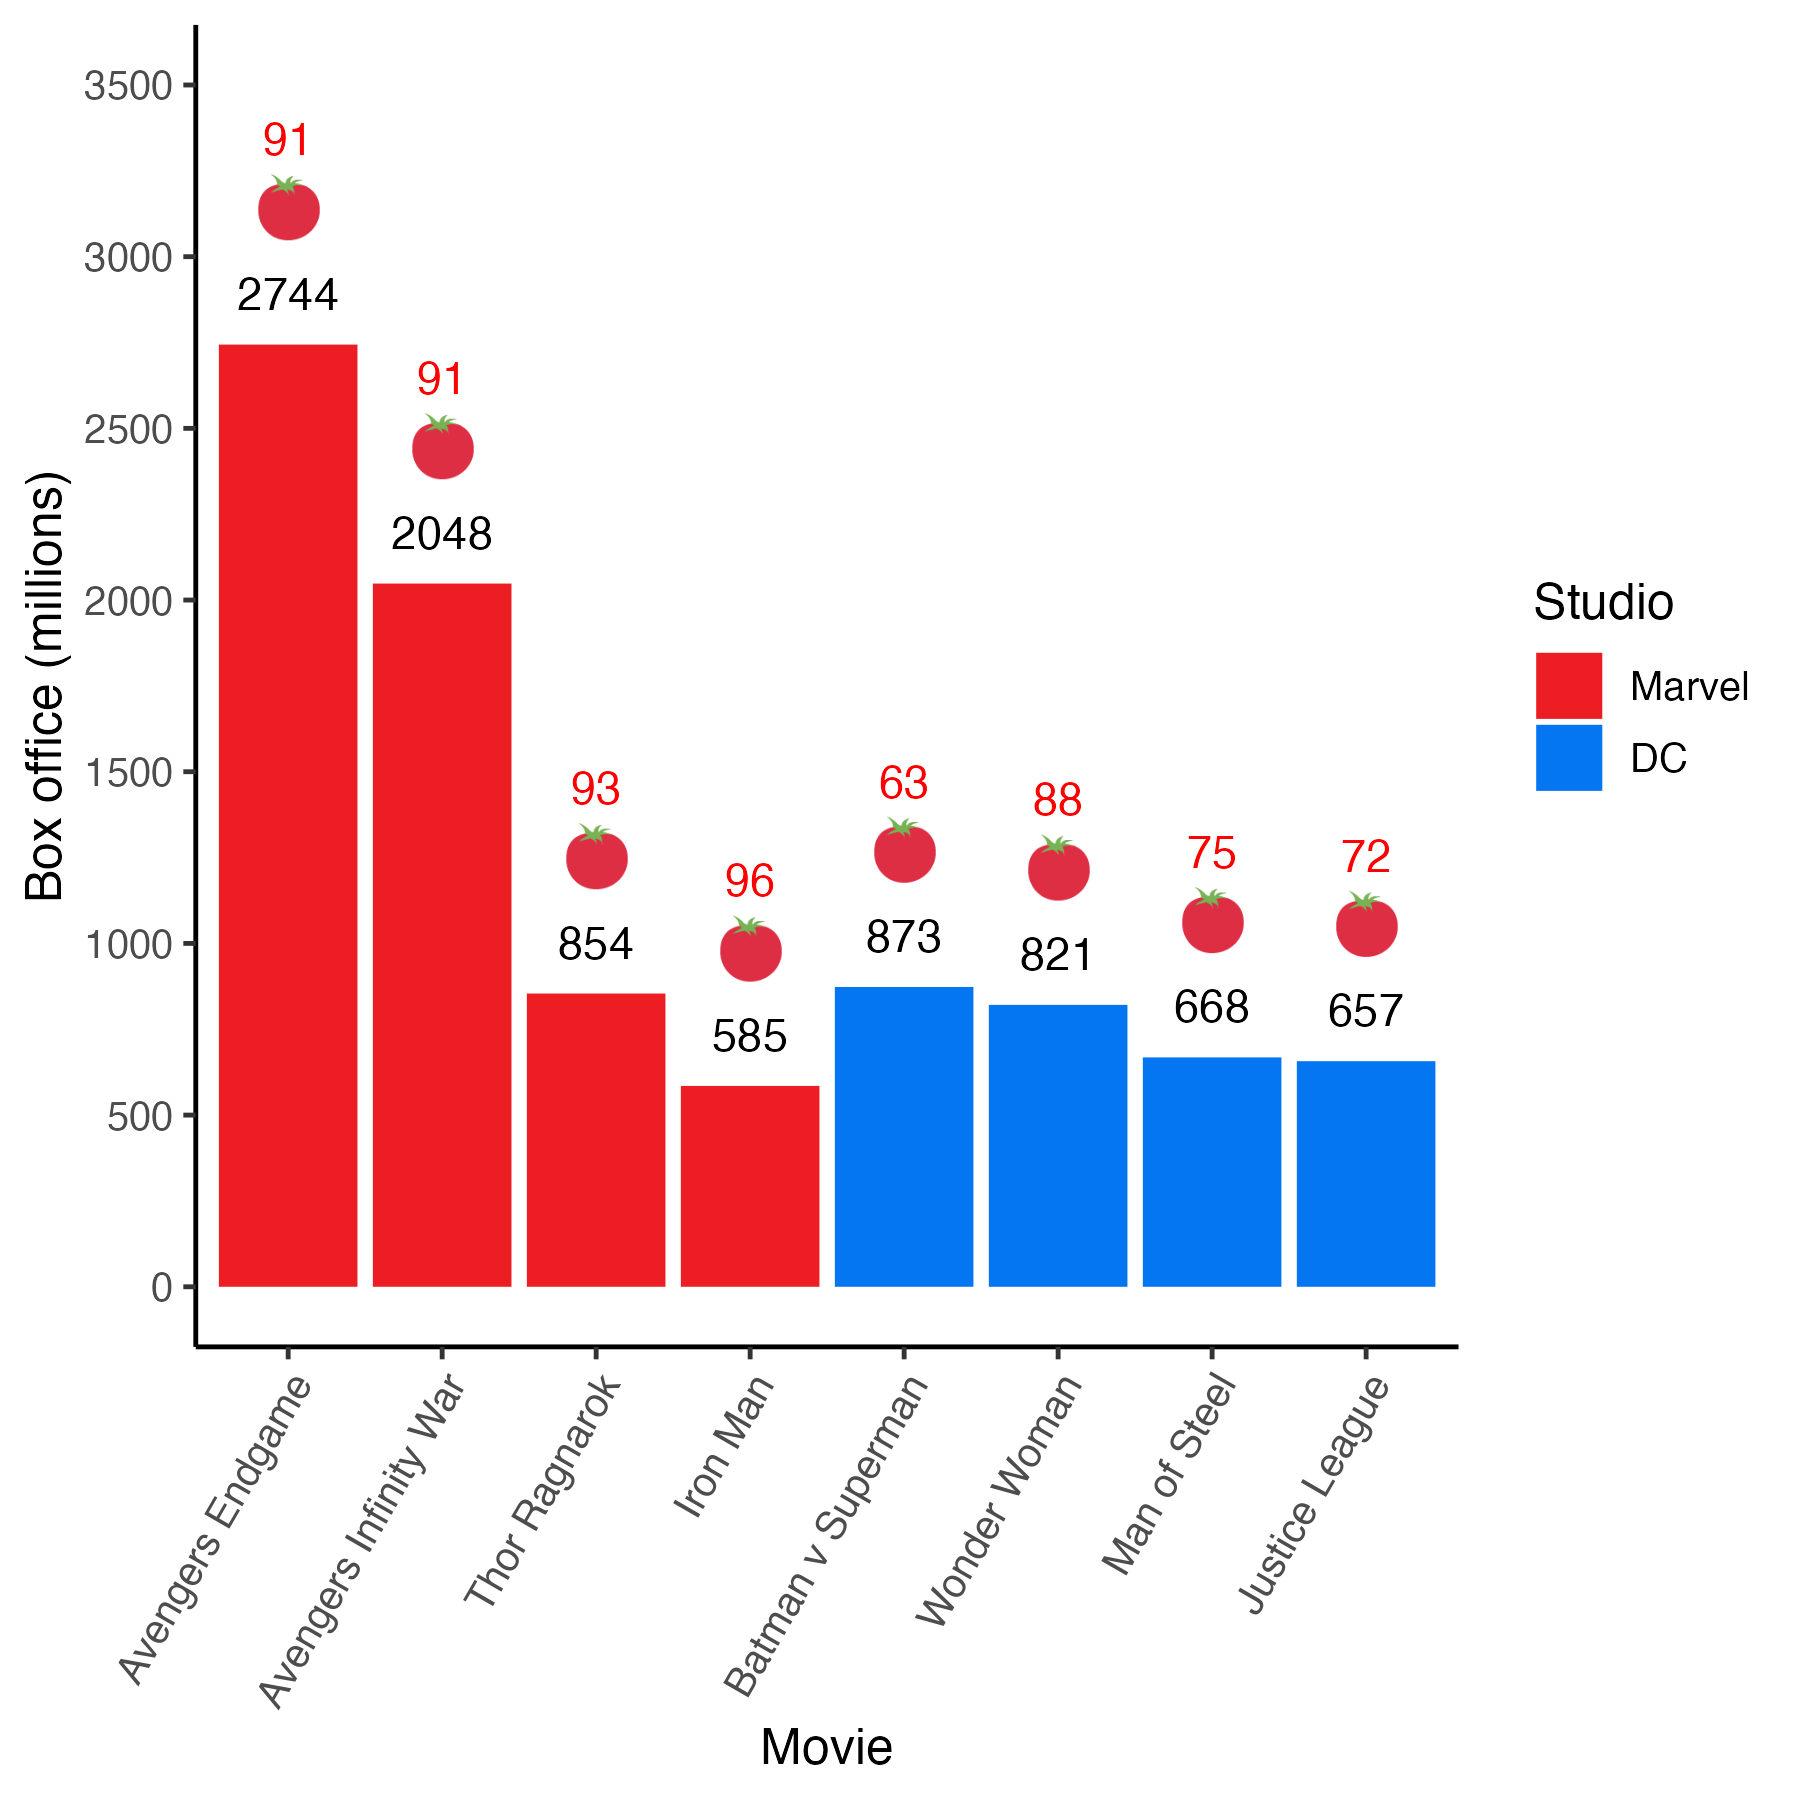
\includegraphics[width=0.65\linewidth]{ch_graphing/images/emoji_graph}

\hypertarget{accessible-colors}{%
\section{Accessible Colors}\label{accessible-colors}}

The current version of the graph is much improved from where we started at the begining of the chapter. One notable improvement was the use of the ``proper'' colors for the Marvel and DC studios. Although using these colors was aethetically pleasing, a major consideration is ensuring your graphs are accessible to a wide audience.

Color blindness is an issue that affects approximately five percent of the population. A nuanced discussion of the different types of color blindness is beyond the scope of this chapter. We can, however, take a momement to think about every graph as being composed of two parts that work together to create the colors overall image. We can think of there being a lightness (i.e., light vs.~dark) component and a hue component (e.g., magenta, yellow, etc.). Together these two components work together to create colors that we see. This distinction between lightness and hue is relevant to all images not just graphs \citep[see][]{margulis2005photoshop}.

\begin{figure}
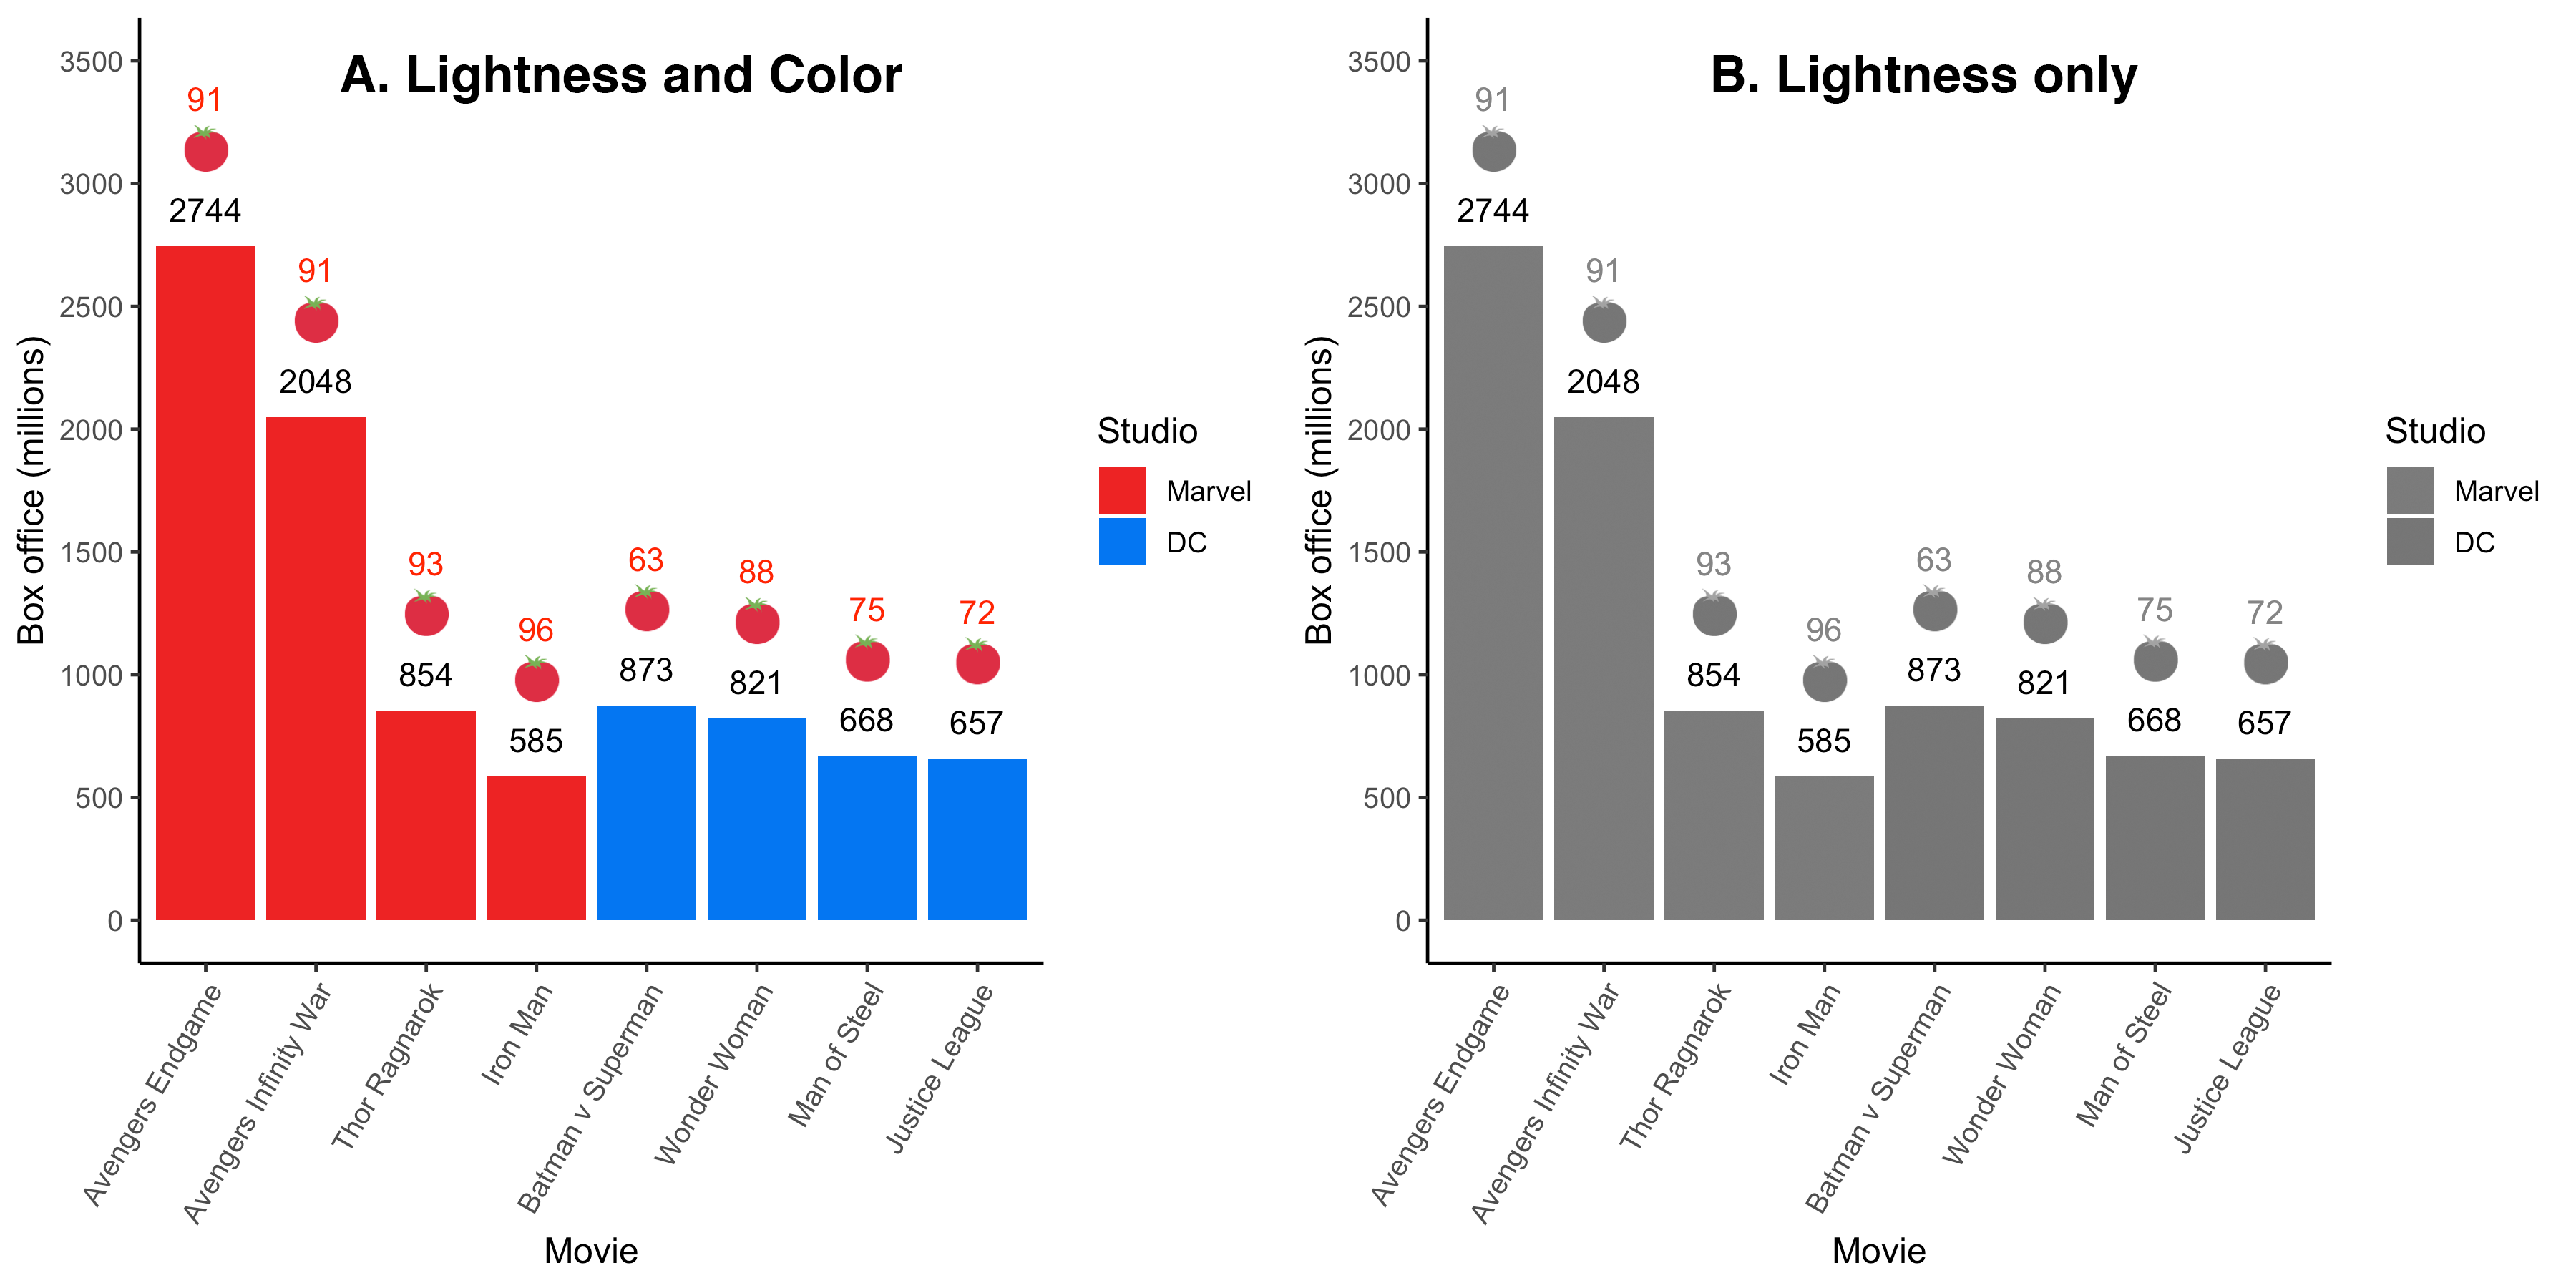
\includegraphics[width=0.75\linewidth]{ch_graphing/images/nocolorcomparison} \caption{Hue removed from current graph}\label{fig:colorcomparison}
\end{figure}

Figure \ref{fig:colorcomparison}A presents our current graph whereas Figure \ref{fig:colorcomparison}B presents the same graph with the hue component removed. You can see that when the hue component is removed that the distinction between the Marvel and DC bars is also removed. The particular colors used to represent Marvel/DC differ in terms of hue but not lightness. Consequently, when we remove the hue component we are left with a graph, \ref{fig:colorcomparison}B, that does not differentiate between the two studios. In order for a color graph to be accessible to people with color blindness we need to pick colors that vary in terms of lightness as well as hue. We can do that with the help of the RColorBrewer package.

\hypertarget{rcolorbrewer}{%
\subsection{RColorBrewer}\label{rcolorbrewer}}

\hypertarget{picking-a-palette}{%
\subsubsection{Picking a palette}\label{picking-a-palette}}

The RColorBrewer package can be used to generate color palettes for graphs that are accessible to people with color blindness. That is, it creates sets of colors, called palettes, for which the colors vary in terms of both lightness and hue. You can see the color-blind accessible palettes, along with their respective names, by using the command below. This code produces a wide range of color-blind accessible palettes with a large number of colors in each palette - as illustrated in Figure \ref{fig:colorpal}.

\begin{Shaded}
\begin{Highlighting}[]
\KeywordTok{library}\NormalTok{(RColorBrewer)}
\KeywordTok{display.brewer.all}\NormalTok{(}\DataTypeTok{n =} \OtherTok{NULL}\NormalTok{, }\DataTypeTok{colorblindFriendly =} \OtherTok{TRUE}\NormalTok{)}
\end{Highlighting}
\end{Shaded}

\begin{figure}
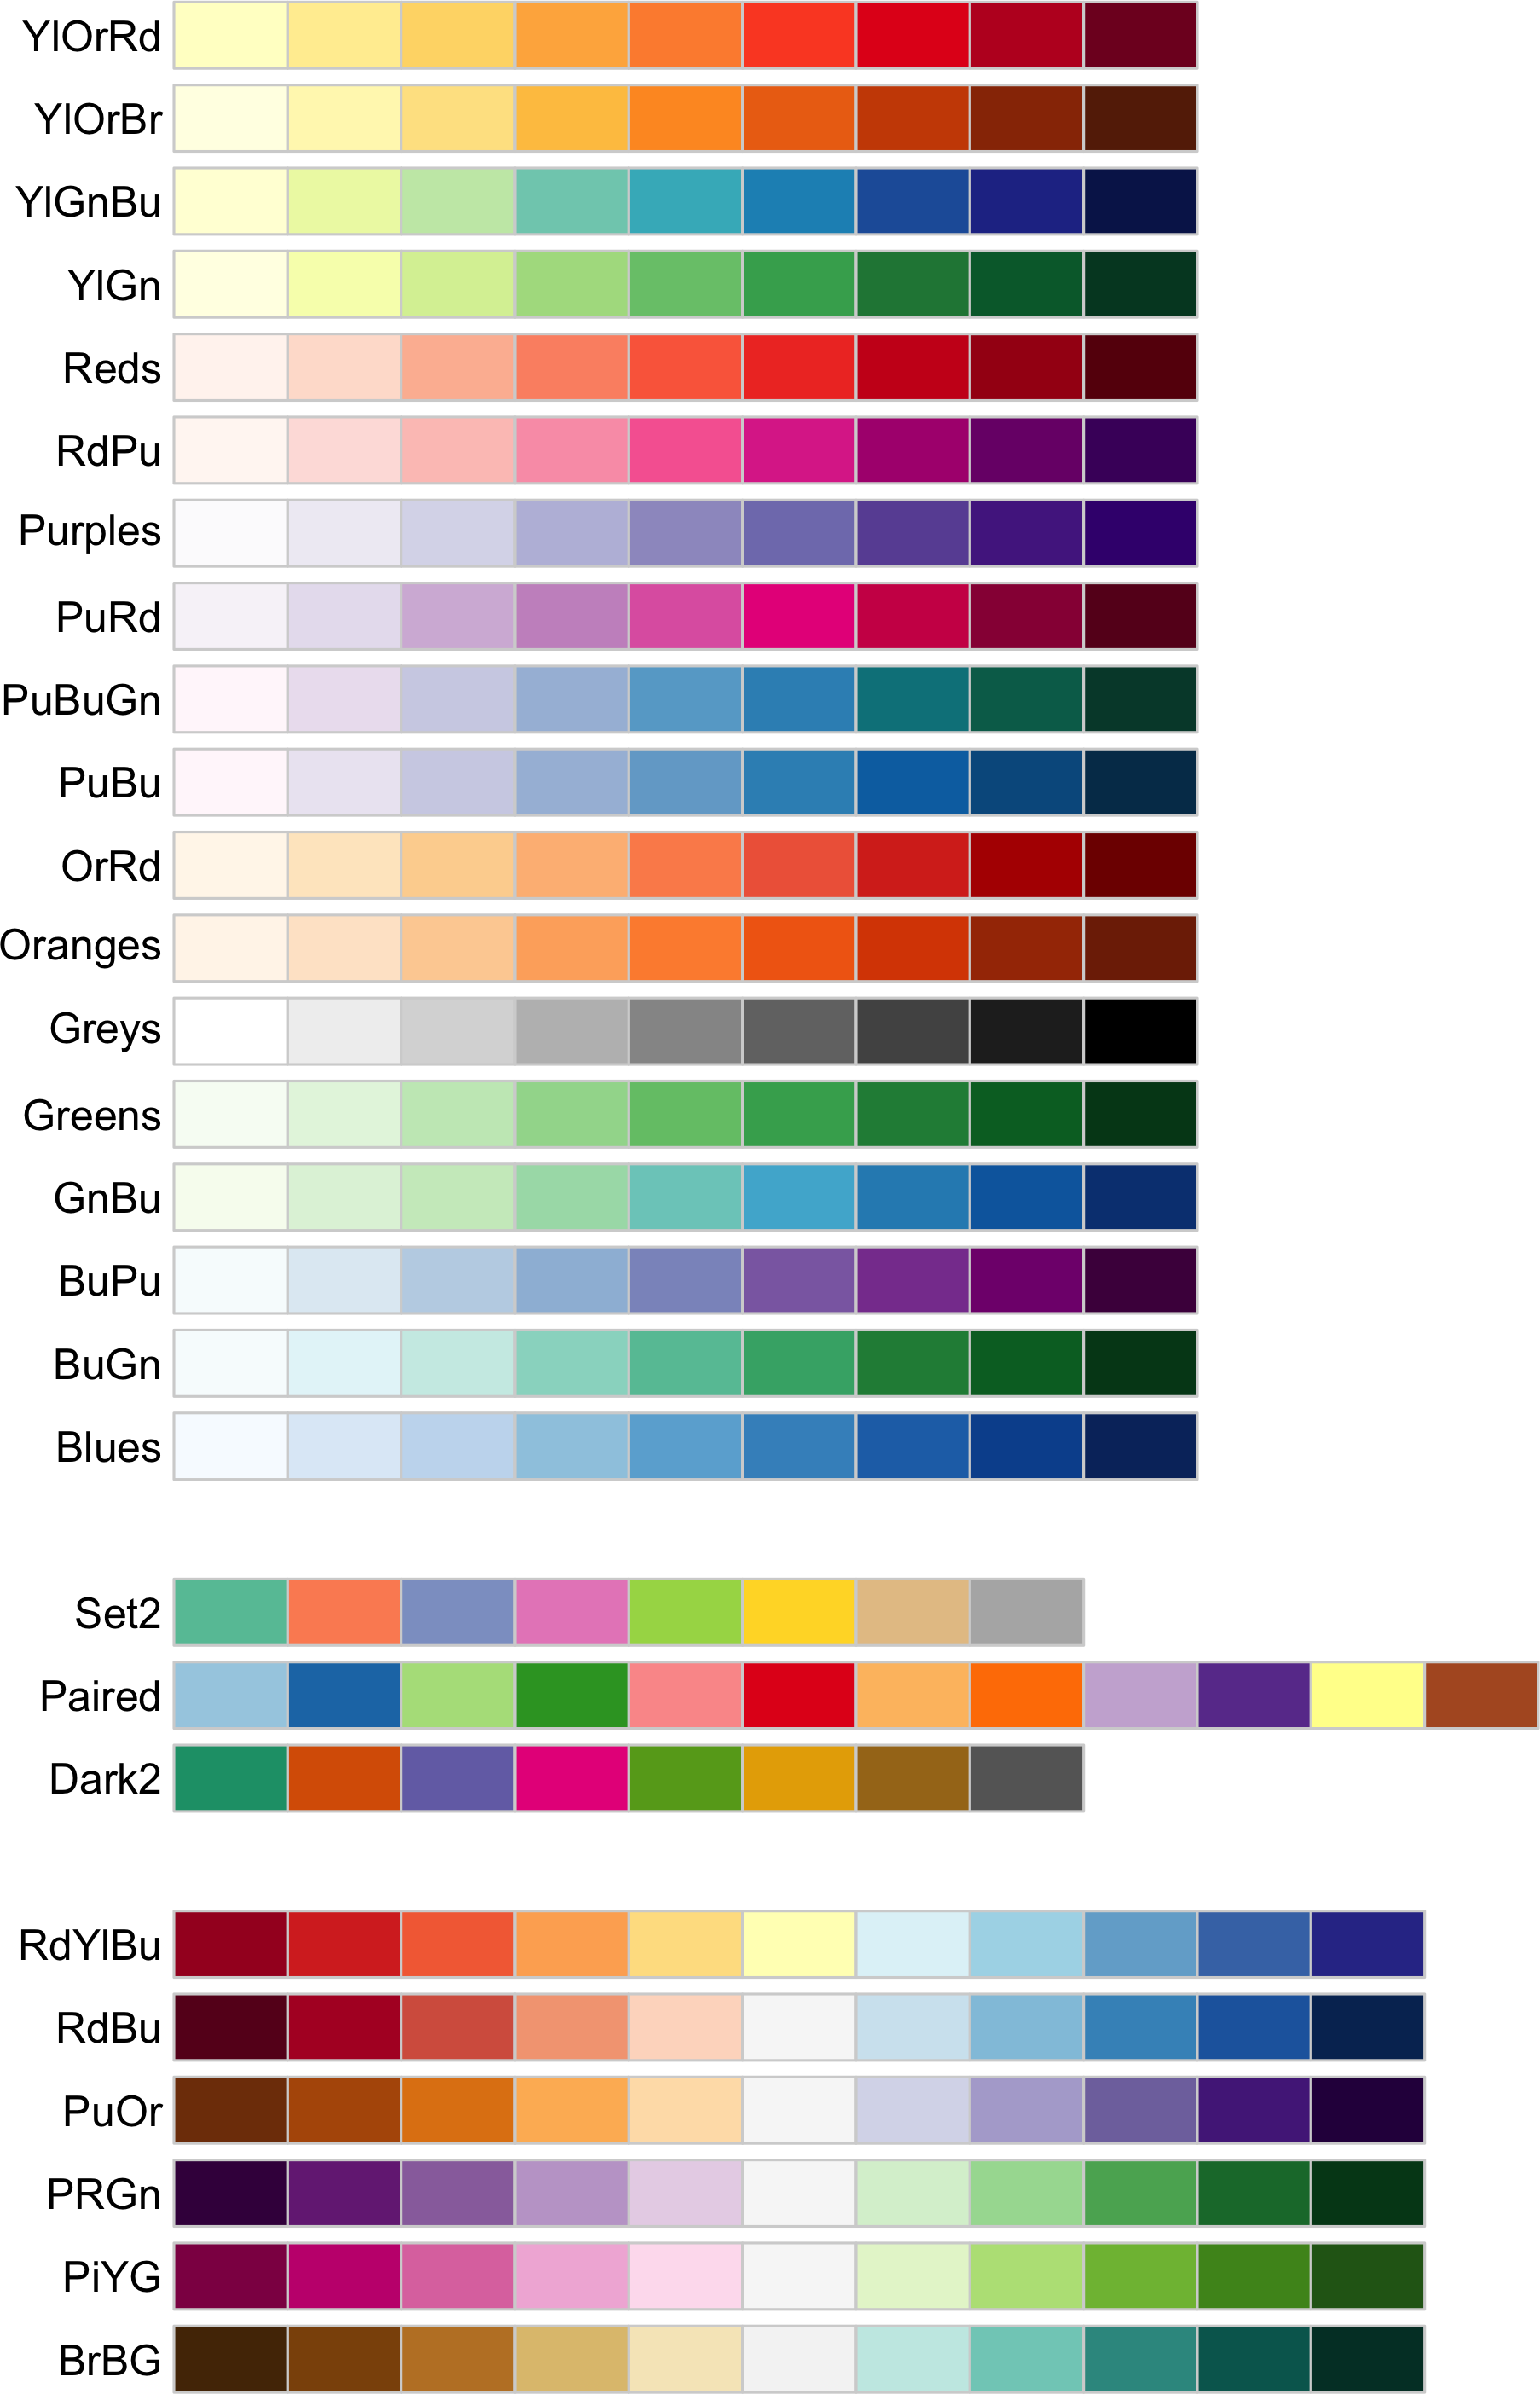
\includegraphics[width=0.7\linewidth,height=0.7\textheight]{ch_graphing/images/colors_all} \caption{Wide range color palette (color-blind accessible)}\label{fig:colorpal}
\end{figure}

\newpage

In Figure \ref{fig:colorpal}, above, we showed palettes with a large number of colors. But if you have a smaller number of possible colors in your graph - you want a palette with fewer colors (to ensure maximum contrast between those colors). You can, for example, obtain palettes with only three colors using the code below.

\begin{Shaded}
\begin{Highlighting}[]
\KeywordTok{library}\NormalTok{(RColorBrewer)}
\KeywordTok{display.brewer.all}\NormalTok{(}\DataTypeTok{n =} \DecValTok{3}\NormalTok{, }\DataTypeTok{colorblindFriendly =} \OtherTok{TRUE}\NormalTok{)}
\end{Highlighting}
\end{Shaded}

The above code generates the three-color palettes presented in Figure \ref{fig:colorspalthree}.

\begin{figure}
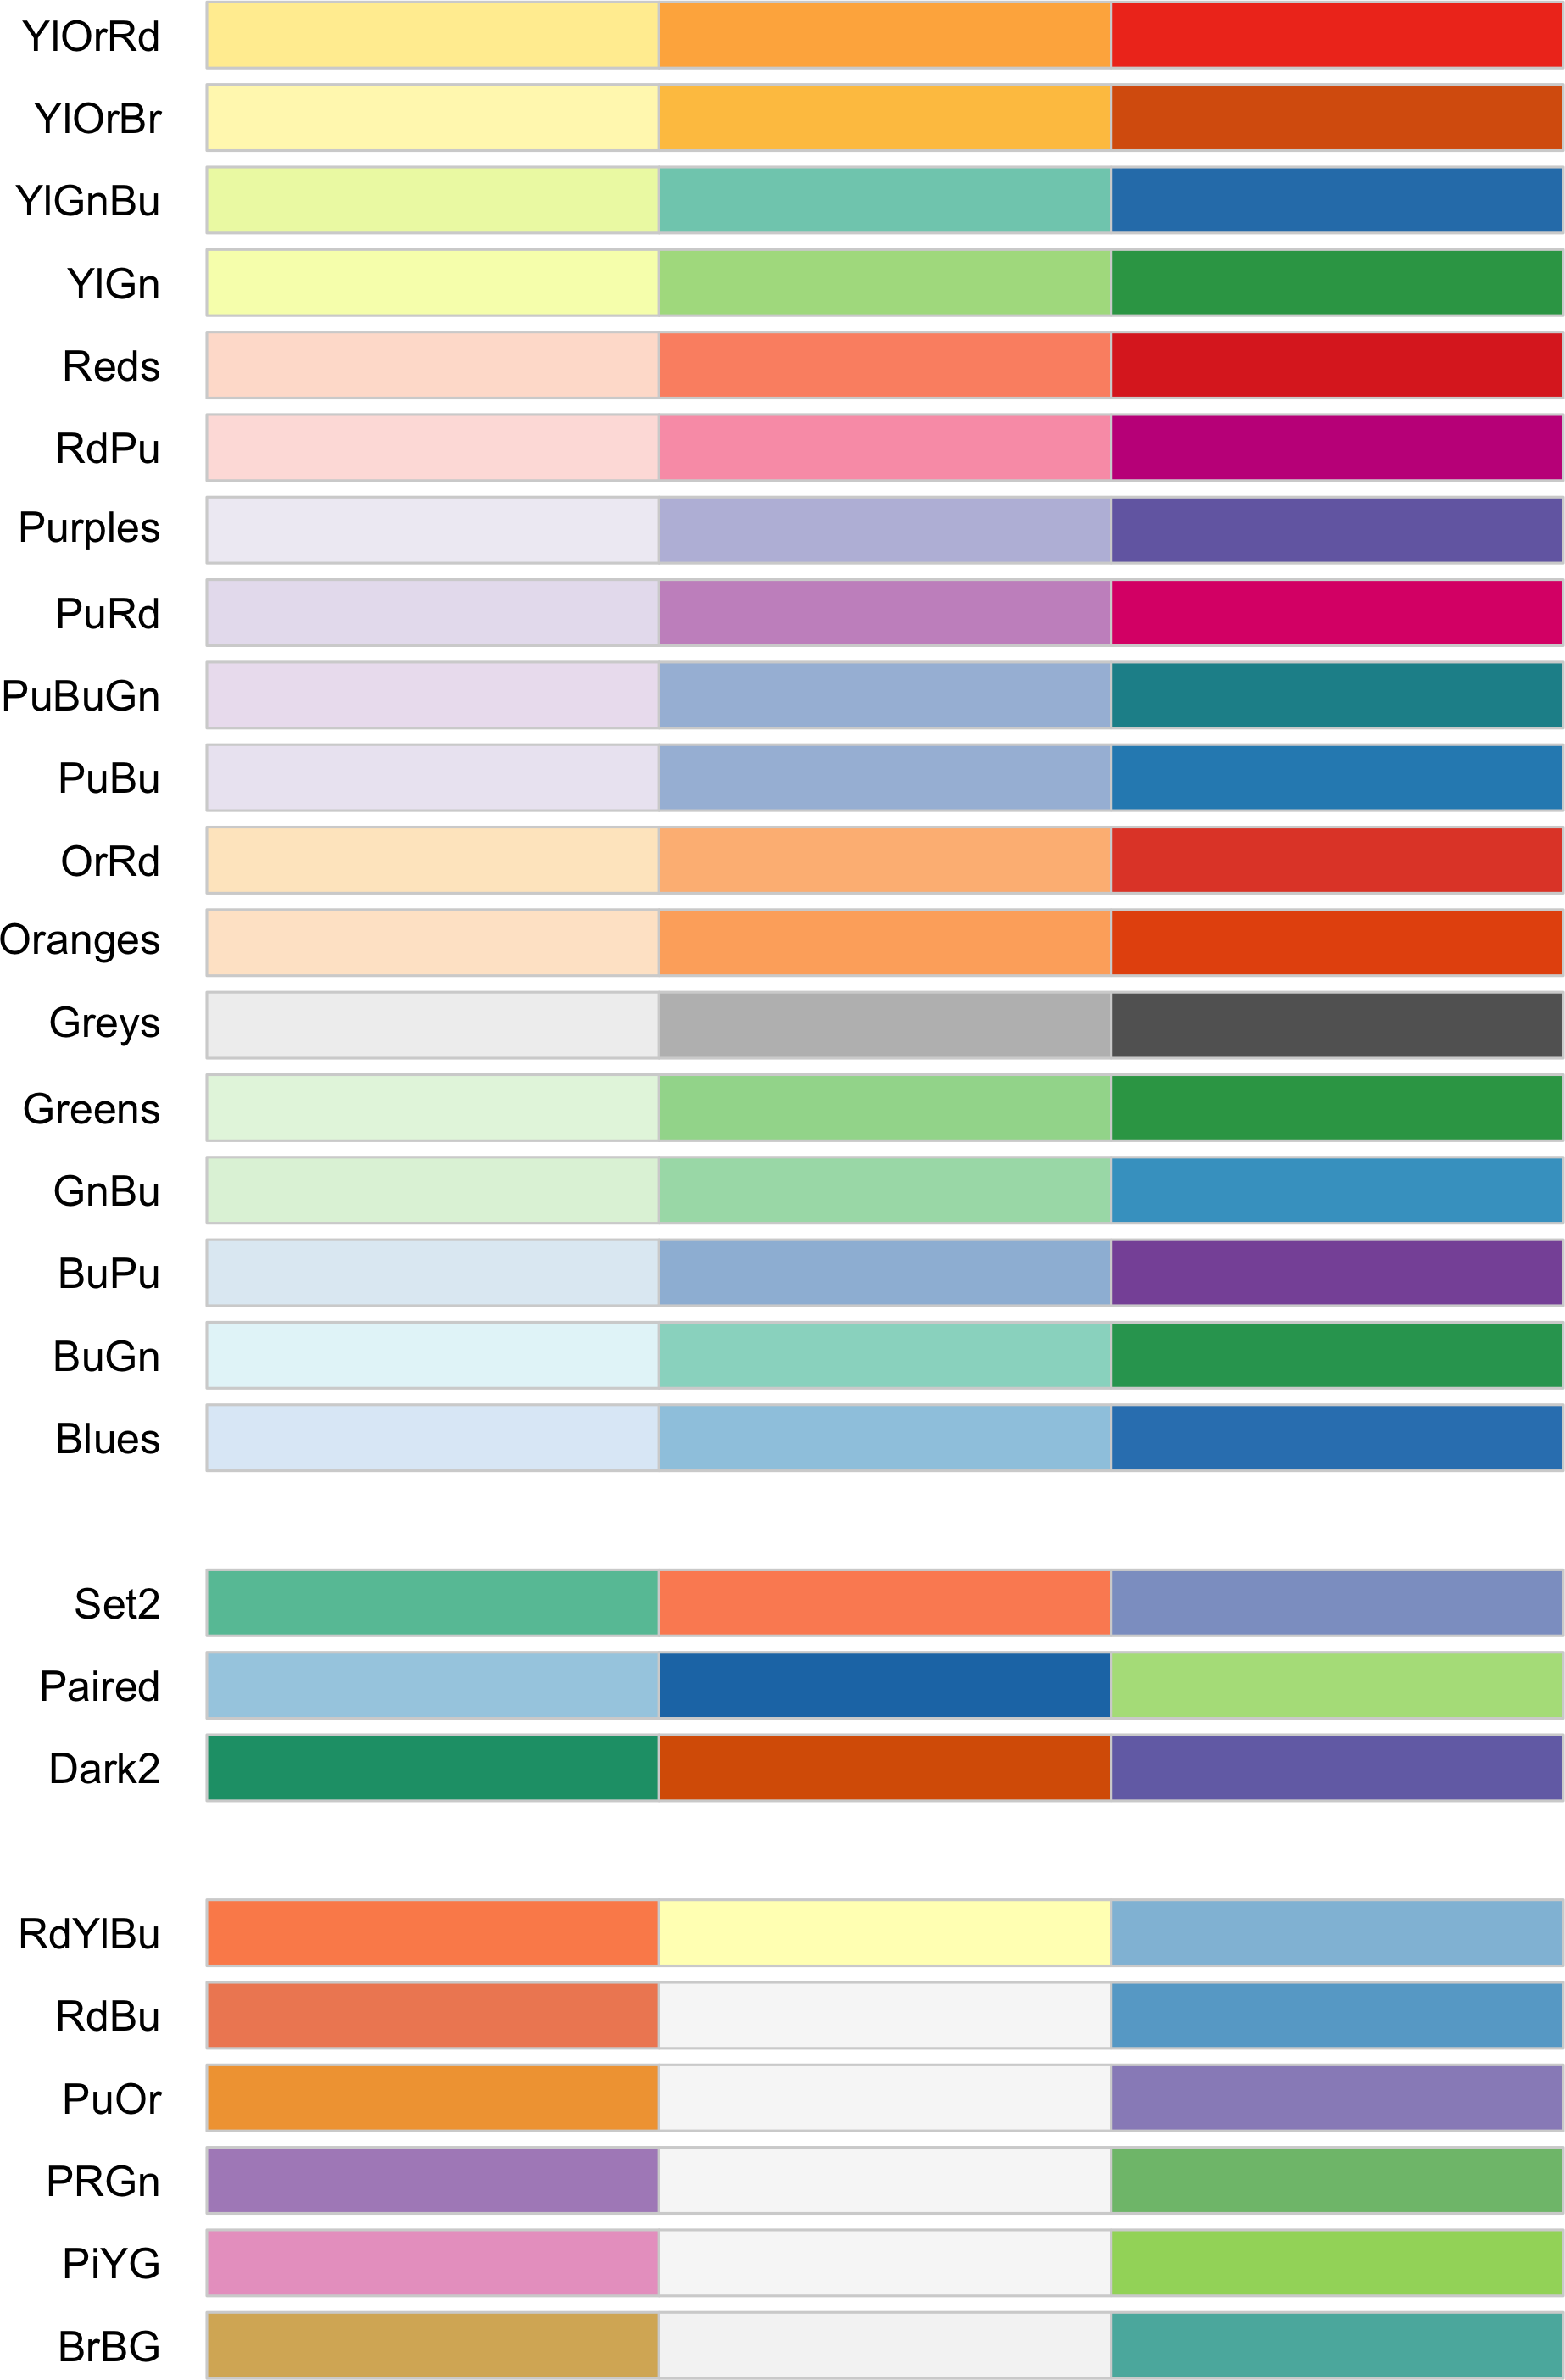
\includegraphics[width=0.7\linewidth,height=0.7\textheight]{ch_graphing/images/colors_3} \caption{Narrow range color palette (color-blind accessible)}\label{fig:colorspalthree}
\end{figure}

\newpage

\hypertarget{using-a-palette}{%
\subsubsection{Using a palette}\label{using-a-palette}}

We can use a color palette by specifying its name within scale\_fill\_brewer(). We want to use the ``Paired'' palette in Figure \ref{fig:colorspalthree} so we use the code: scale\_fill\_brewer(palette = ``Paired''), as illustrated below:

\begin{Shaded}
\begin{Highlighting}[]
\NormalTok{my_graph <-}\StringTok{ }\KeywordTok{ggplot}\NormalTok{(}\DataTypeTok{data =}\NormalTok{ movie_data,}
           \DataTypeTok{mapping =} \KeywordTok{aes}\NormalTok{(}\DataTypeTok{x =}\NormalTok{ title,}
                         \DataTypeTok{y =}\NormalTok{ boxoffice,}
                         \DataTypeTok{label =}\NormalTok{ boxoffice, }
                         \DataTypeTok{fill =}\NormalTok{ studio)) }\OperatorTok{+}
\StringTok{  }\KeywordTok{geom_col}\NormalTok{() }\OperatorTok{+}
\StringTok{  }\KeywordTok{geom_text}\NormalTok{(}\DataTypeTok{nudge_y =} \DecValTok{150}\NormalTok{)  }\OperatorTok{+}
\StringTok{  }\KeywordTok{geom_text}\NormalTok{(}\DataTypeTok{mapping =} \KeywordTok{aes}\NormalTok{(}\DataTypeTok{label =}\NormalTok{ tomatoes_aud), }
            \DataTypeTok{nudge_y =} \DecValTok{600}\NormalTok{, }
            \DataTypeTok{colour =} \StringTok{"red"}\NormalTok{) }\OperatorTok{+}
\StringTok{  }\KeywordTok{geom_emoji}\NormalTok{(}\DataTypeTok{mapping =} \KeywordTok{aes}\NormalTok{(}\DataTypeTok{y =}\NormalTok{ boxoffice }\OperatorTok{+}\StringTok{ }\DecValTok{400}\NormalTok{),}
             \DataTypeTok{emoji=}\StringTok{"1f345"}\NormalTok{) }\OperatorTok{+}
\StringTok{  }\KeywordTok{coord_cartesian}\NormalTok{(}\DataTypeTok{ylim =} \KeywordTok{c}\NormalTok{(}\DecValTok{0}\NormalTok{, }\DecValTok{3500}\NormalTok{)) }\OperatorTok{+}
\StringTok{  }\KeywordTok{scale_y_continuous}\NormalTok{(}\DataTypeTok{breaks =} \KeywordTok{seq}\NormalTok{(}\DecValTok{0}\NormalTok{, }\DecValTok{3500}\NormalTok{, }\DataTypeTok{by =} \DecValTok{500}\NormalTok{)) }\OperatorTok{+}
\StringTok{  }\KeywordTok{labs}\NormalTok{(}\DataTypeTok{x =} \StringTok{"Movie"}\NormalTok{,}
       \DataTypeTok{y =} \StringTok{"Box office (millions)"}\NormalTok{,}
       \DataTypeTok{fill =} \StringTok{"Studio"}\NormalTok{) }\OperatorTok{+}
\StringTok{  }\KeywordTok{theme_classic}\NormalTok{(}\DecValTok{12}\NormalTok{) }\OperatorTok{+}
\StringTok{  }\KeywordTok{theme}\NormalTok{(}\DataTypeTok{axis.text.x =} \KeywordTok{element_text}\NormalTok{(}\DataTypeTok{angle =} \DecValTok{60}\NormalTok{, }
                                   \DataTypeTok{hjust =} \DecValTok{1}\NormalTok{)) }\OperatorTok{+}
\StringTok{  }\KeywordTok{scale_fill_brewer}\NormalTok{(}\DataTypeTok{palette =} \StringTok{"Paired"}\NormalTok{)}
\end{Highlighting}
\end{Shaded}

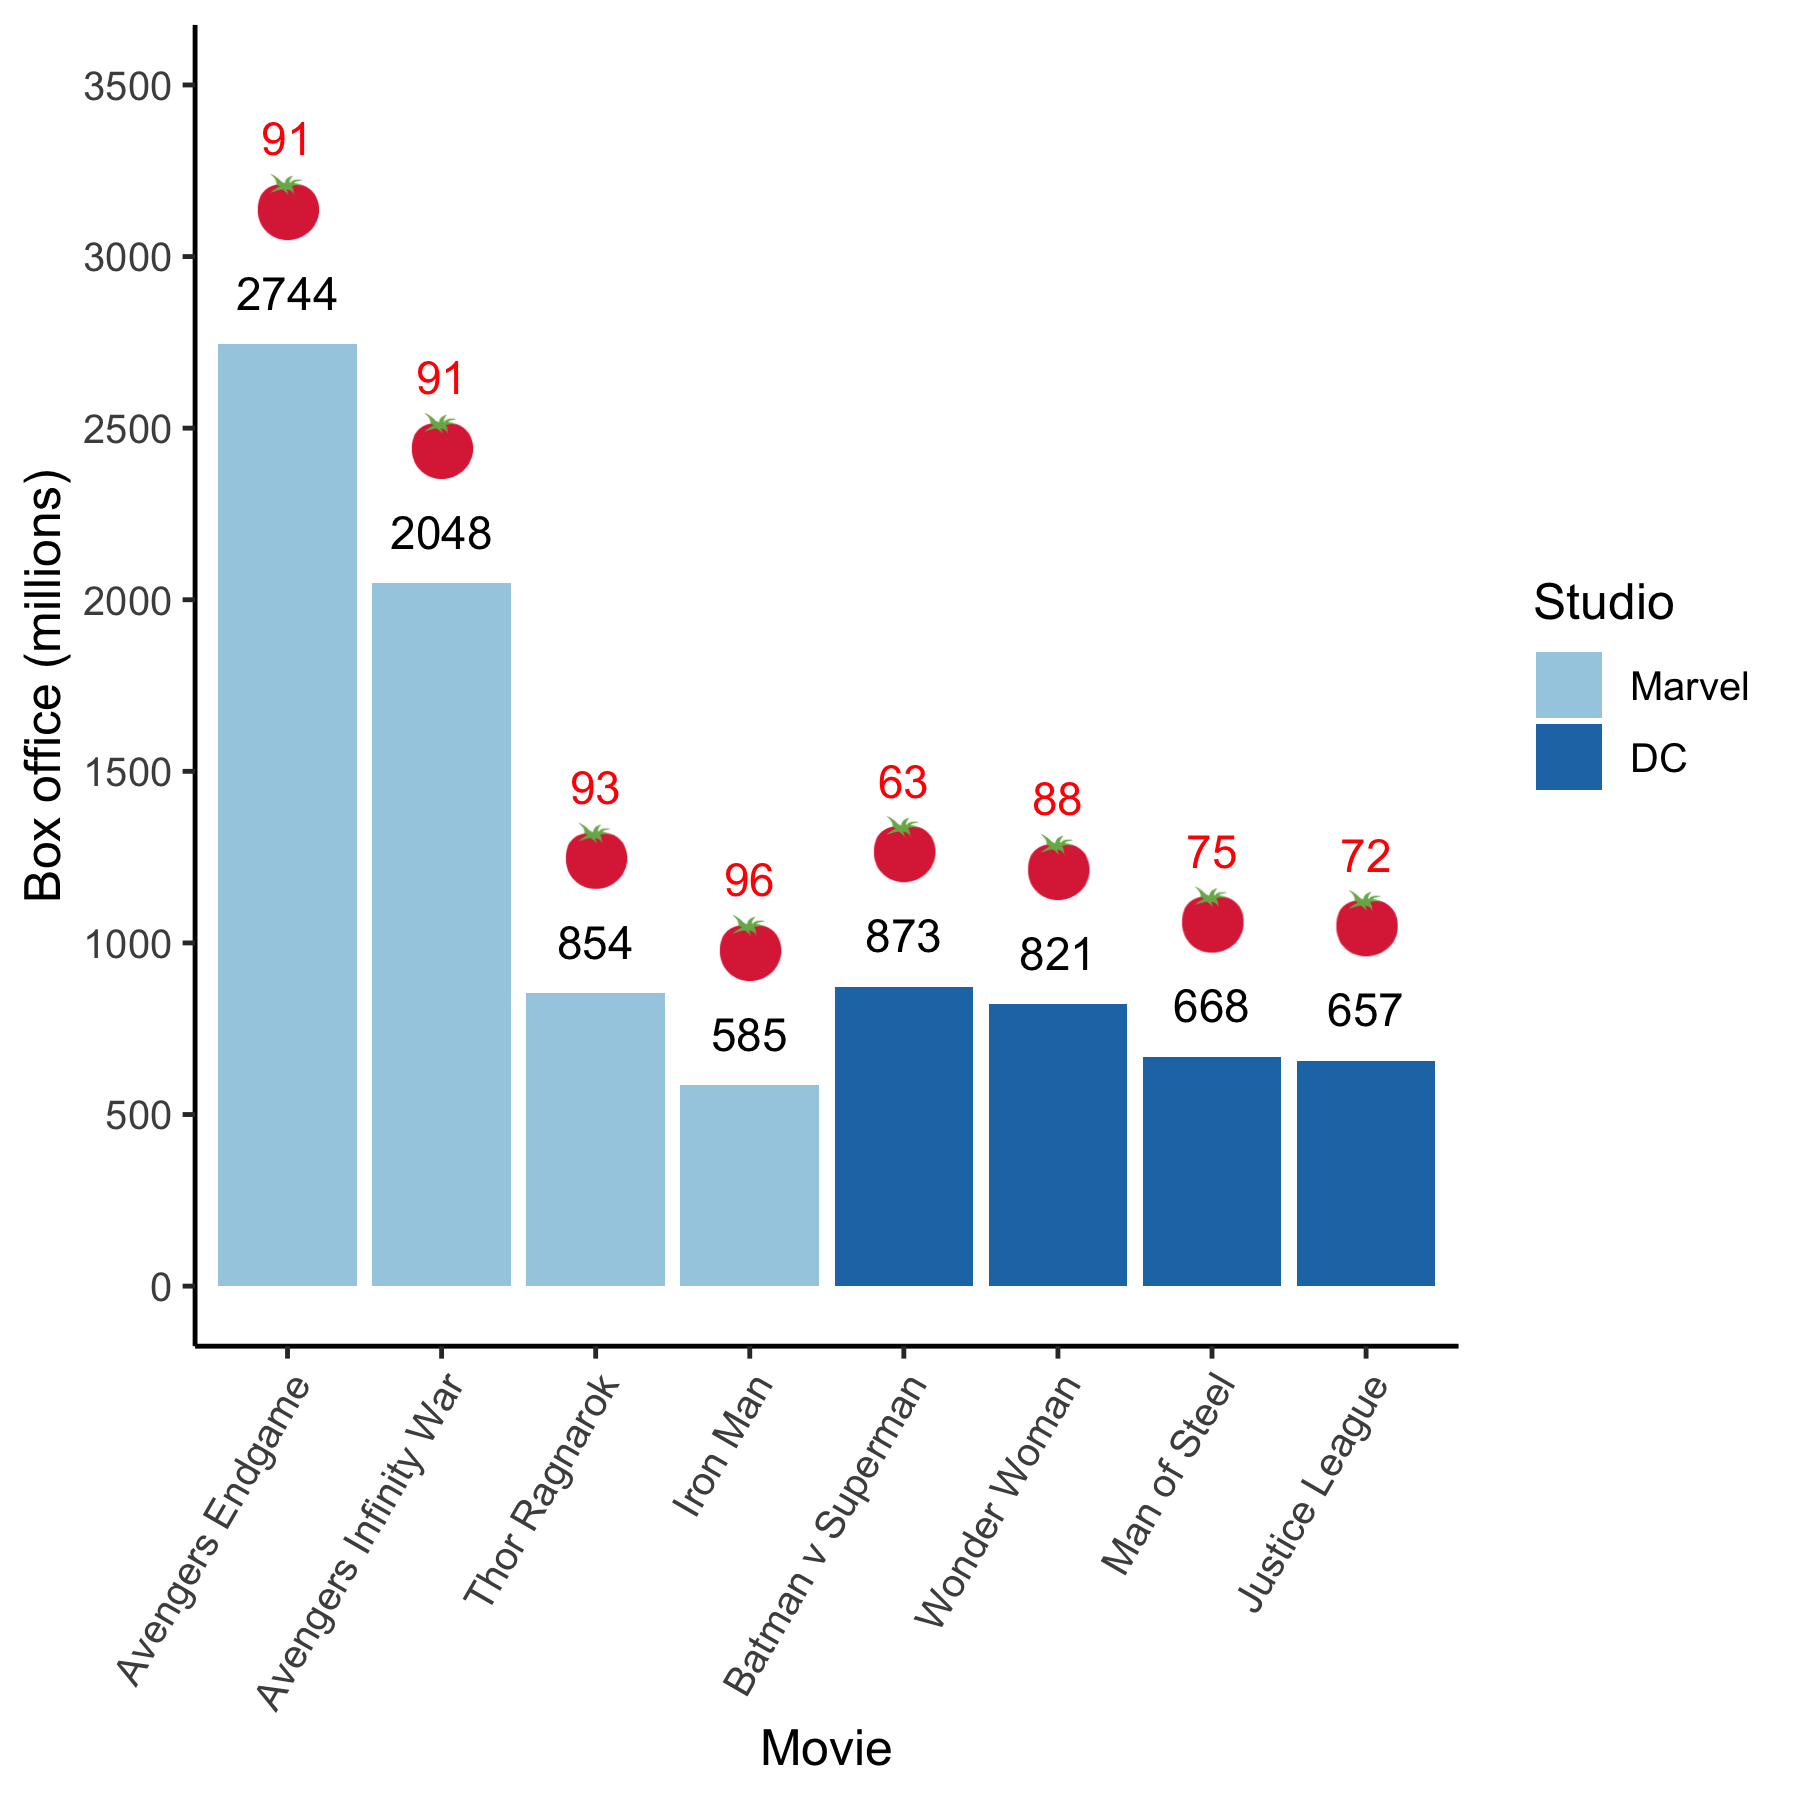
\includegraphics[width=0.65\linewidth]{ch_graphing/images/emoji_graph4}

\hypertarget{palette-subsets}{%
\subsubsection{Palette subsets}\label{palette-subsets}}

Our graph had only two colors but the ``Paired'' palette had three colors. When ggplot made the graph it automatically used the first two colors of the three color palette. What if you wanted the second two colors in the palette? We can do that but we have to revert to a manual color process like we used before via the scale\_fill\_manual(). But we want to do so using the colors from the ``Paired'' palette. We can obtain the color codes for the ``Paired'' palette with the code below:

\begin{Shaded}
\begin{Highlighting}[]
\KeywordTok{brewer.pal}\NormalTok{(}\DataTypeTok{n =} \DecValTok{3}\NormalTok{, }\DataTypeTok{name =} \StringTok{"Paired"}\NormalTok{)}
\end{Highlighting}
\end{Shaded}

\begin{verbatim}
## [1] "#A6CEE3" "#1F78B4" "#B2DF8A"
\end{verbatim}

The numbers in the output correspond to values representing the three colors of the ``Paired'' palette, see Figure \ref{fig:pairedpal}. If we want the last two colors in the palette for our graph that means we want the colors: \#1F78B4 and \#B2DF8A.

\begin{figure}
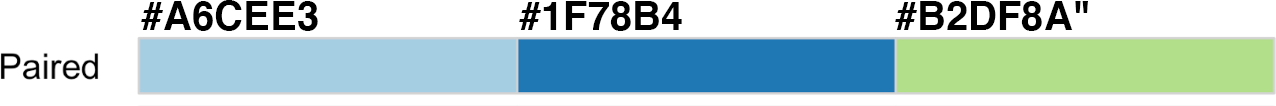
\includegraphics[width=0.75\linewidth]{ch_graphing/images/pairedpalette} \caption{Paired palette colors with hex numbers}\label{fig:pairedpal}
\end{figure}

We can put the two colors we want (\#1F78B4 and \#B2DF8A) on the graph by using the scale\_fill\_manual() command - instead of the scale\_fill\_brewer() command. We can see this in the code below:

\begin{Shaded}
\begin{Highlighting}[]
\NormalTok{my_graph <-}\StringTok{ }\KeywordTok{ggplot}\NormalTok{(}\DataTypeTok{data =}\NormalTok{ movie_data,}
           \DataTypeTok{mapping =} \KeywordTok{aes}\NormalTok{(}\DataTypeTok{x =}\NormalTok{ title,}
                         \DataTypeTok{y =}\NormalTok{ boxoffice,}
                         \DataTypeTok{label =}\NormalTok{ boxoffice, }
                         \DataTypeTok{fill =}\NormalTok{ studio)) }\OperatorTok{+}
\StringTok{  }\KeywordTok{geom_col}\NormalTok{() }\OperatorTok{+}
\StringTok{  }\KeywordTok{geom_text}\NormalTok{(}\DataTypeTok{nudge_y =} \DecValTok{150}\NormalTok{)  }\OperatorTok{+}
\StringTok{  }\KeywordTok{geom_text}\NormalTok{(}\DataTypeTok{mapping =} \KeywordTok{aes}\NormalTok{(}\DataTypeTok{label =}\NormalTok{ tomatoes_aud), }
            \DataTypeTok{nudge_y =} \DecValTok{600}\NormalTok{, }
            \DataTypeTok{colour =} \StringTok{"red"}\NormalTok{) }\OperatorTok{+}
\StringTok{  }\KeywordTok{geom_emoji}\NormalTok{(}\DataTypeTok{mapping =} \KeywordTok{aes}\NormalTok{(}\DataTypeTok{y =}\NormalTok{ boxoffice }\OperatorTok{+}\StringTok{ }\DecValTok{400}\NormalTok{),}
             \DataTypeTok{emoji=}\StringTok{"1f345"}\NormalTok{) }\OperatorTok{+}
\StringTok{  }\KeywordTok{coord_cartesian}\NormalTok{(}\DataTypeTok{ylim =} \KeywordTok{c}\NormalTok{(}\DecValTok{0}\NormalTok{, }\DecValTok{3500}\NormalTok{)) }\OperatorTok{+}
\StringTok{  }\KeywordTok{scale_y_continuous}\NormalTok{(}\DataTypeTok{breaks =} \KeywordTok{seq}\NormalTok{(}\DecValTok{0}\NormalTok{, }\DecValTok{3500}\NormalTok{, }\DataTypeTok{by =} \DecValTok{500}\NormalTok{)) }\OperatorTok{+}
\StringTok{  }\KeywordTok{labs}\NormalTok{(}\DataTypeTok{x =} \StringTok{"Movie"}\NormalTok{,}
       \DataTypeTok{y =} \StringTok{"Box office (millions)"}\NormalTok{,}
       \DataTypeTok{fill =} \StringTok{"Studio"}\NormalTok{) }\OperatorTok{+}
\StringTok{  }\KeywordTok{theme_classic}\NormalTok{(}\DecValTok{12}\NormalTok{) }\OperatorTok{+}
\StringTok{  }\KeywordTok{theme}\NormalTok{(}\DataTypeTok{axis.text.x =} \KeywordTok{element_text}\NormalTok{(}\DataTypeTok{angle =} \DecValTok{60}\NormalTok{, }
                                   \DataTypeTok{hjust =} \DecValTok{1}\NormalTok{)) }\OperatorTok{+}
\StringTok{  }\KeywordTok{scale_fill_manual}\NormalTok{(}\DataTypeTok{values =} \KeywordTok{c}\NormalTok{(}\StringTok{"#1F78B4"}\NormalTok{, }\StringTok{"#B2DF8A"}\NormalTok{))}
\end{Highlighting}
\end{Shaded}

\includegraphics[width=0.65\linewidth]{ch_graphing/images/emoji_graph5}

Now that we have used a color-blind accessible palette in the graph we can look at the graph without the hue component. In Figure \ref{fig:colorcomparison2}B, below, notice that the bars representing the two studios are easily distinguishable based on lightness alone. That is, the lightness graph in Figure \ref{fig:colorcomparison2}B demonstrates the new color-blind accessible colors vary in term of both hue and lightness - not just hue. Therefore, when hue is removed the two colors are distinguishable. This makes the graph accessible to color-blind individuals.

\begin{figure}
\includegraphics[width=0.75\linewidth]{ch_graphing/images/nocolorcomparison2} \caption{Color information (i.e., hue) removed from new color-blind accessible graph}\label{fig:colorcomparison2}
\end{figure}

\hypertarget{avoid-color}{%
\subsection{Avoid color}\label{avoid-color}}

When you only have two colors on a graph another option for creating an accessible graph is to remove the colors entirely and make a black and white graph. In the code below we use scale\_fill\_manual() with the values ``\#ffffff'' (white) and "``\#000000'' (black). The intent was to create bars that are white for Marvel and black for DC. Unfortunately, because the graph has a white background you can see this resulted in the Marvel bars disappearing.

\begin{Shaded}
\begin{Highlighting}[]
\NormalTok{my_graph <-}\StringTok{ }\KeywordTok{ggplot}\NormalTok{(}\DataTypeTok{data =}\NormalTok{ movie_data,}
           \DataTypeTok{mapping =} \KeywordTok{aes}\NormalTok{(}\DataTypeTok{x =}\NormalTok{ title,}
                         \DataTypeTok{y =}\NormalTok{ boxoffice,}
                         \DataTypeTok{label =}\NormalTok{ boxoffice, }
                         \DataTypeTok{fill =}\NormalTok{ studio)) }\OperatorTok{+}
\StringTok{  }\KeywordTok{geom_col}\NormalTok{() }\OperatorTok{+}
\StringTok{  }\KeywordTok{geom_text}\NormalTok{(}\DataTypeTok{nudge_y =} \DecValTok{150}\NormalTok{)  }\OperatorTok{+}
\StringTok{  }\KeywordTok{geom_text}\NormalTok{(}\DataTypeTok{mapping =} \KeywordTok{aes}\NormalTok{(}\DataTypeTok{label =}\NormalTok{ tomatoes_aud), }
            \DataTypeTok{nudge_y =} \DecValTok{600}\NormalTok{, }
            \DataTypeTok{colour =} \StringTok{"red"}\NormalTok{) }\OperatorTok{+}
\StringTok{  }\KeywordTok{geom_emoji}\NormalTok{(}\DataTypeTok{mapping =} \KeywordTok{aes}\NormalTok{(}\DataTypeTok{y =}\NormalTok{ boxoffice }\OperatorTok{+}\StringTok{ }\DecValTok{400}\NormalTok{),}
             \DataTypeTok{emoji=}\StringTok{"1f345"}\NormalTok{) }\OperatorTok{+}
\StringTok{  }\KeywordTok{coord_cartesian}\NormalTok{(}\DataTypeTok{ylim =} \KeywordTok{c}\NormalTok{(}\DecValTok{0}\NormalTok{, }\DecValTok{3500}\NormalTok{)) }\OperatorTok{+}
\StringTok{  }\KeywordTok{scale_y_continuous}\NormalTok{(}\DataTypeTok{breaks =} \KeywordTok{seq}\NormalTok{(}\DecValTok{0}\NormalTok{, }\DecValTok{3500}\NormalTok{, }\DataTypeTok{by =} \DecValTok{500}\NormalTok{)) }\OperatorTok{+}
\StringTok{  }\KeywordTok{labs}\NormalTok{(}\DataTypeTok{x =} \StringTok{"Movie"}\NormalTok{,}
       \DataTypeTok{y =} \StringTok{"Box office (millions)"}\NormalTok{,}
       \DataTypeTok{fill =} \StringTok{"Studio"}\NormalTok{) }\OperatorTok{+}
\StringTok{  }\KeywordTok{theme_classic}\NormalTok{(}\DecValTok{12}\NormalTok{) }\OperatorTok{+}
\StringTok{  }\KeywordTok{theme}\NormalTok{(}\DataTypeTok{axis.text.x =} \KeywordTok{element_text}\NormalTok{(}\DataTypeTok{angle =} \DecValTok{60}\NormalTok{, }
                                   \DataTypeTok{hjust =} \DecValTok{1}\NormalTok{)) }\OperatorTok{+}
\StringTok{  }\KeywordTok{scale_fill_manual}\NormalTok{(}\DataTypeTok{values =} \KeywordTok{c}\NormalTok{(}\StringTok{"#ffffff"}\NormalTok{, }\StringTok{"#000000"}\NormalTok{))}
\end{Highlighting}
\end{Shaded}

\includegraphics[width=0.65\linewidth]{ch_graphing/images/emoji_graph2}

How do we get around the Marvel bars disappearing when we use white?

\textbf{Color vs.~fill.} The ggplot packages makes a distinction between \textbf{fill} and \textbf{color}. The term \textbf{fill} is used to refer to the inside color of bars. In contrast, \textbf{color} is used to the refer to the lines that outline the shape of each bar. In the previous code we used fill to change the colors of the bars but we did not use the ``color'' argument in a command. In the code below, we modify the geom\_col() command to use the ``color'' argument. Specifically, we change geom\_col() to geom\_col(color = ``black''). This change adds a black outline around all the bars -- including the ones with a white fill. You can see the result is a much improved graph. This black/white graph is accessible to everyone.

\begin{Shaded}
\begin{Highlighting}[]
\NormalTok{my_graph <-}\StringTok{ }\KeywordTok{ggplot}\NormalTok{(}\DataTypeTok{data =}\NormalTok{ movie_data,}
           \DataTypeTok{mapping =} \KeywordTok{aes}\NormalTok{(}\DataTypeTok{x =}\NormalTok{ title,}
                         \DataTypeTok{y =}\NormalTok{ boxoffice,}
                         \DataTypeTok{label =}\NormalTok{ boxoffice, }
                         \DataTypeTok{fill =}\NormalTok{ studio)) }\OperatorTok{+}
\StringTok{  }\KeywordTok{geom_col}\NormalTok{(}\DataTypeTok{color =} \StringTok{"black"}\NormalTok{) }\OperatorTok{+}
\StringTok{  }\KeywordTok{geom_text}\NormalTok{(}\DataTypeTok{nudge_y =} \DecValTok{150}\NormalTok{)  }\OperatorTok{+}
\StringTok{  }\KeywordTok{geom_text}\NormalTok{(}\DataTypeTok{mapping =} \KeywordTok{aes}\NormalTok{(}\DataTypeTok{label =}\NormalTok{ tomatoes_aud), }
            \DataTypeTok{nudge_y =} \DecValTok{600}\NormalTok{, }
            \DataTypeTok{colour =} \StringTok{"red"}\NormalTok{) }\OperatorTok{+}
\StringTok{  }\KeywordTok{geom_emoji}\NormalTok{(}\DataTypeTok{mapping =} \KeywordTok{aes}\NormalTok{(}\DataTypeTok{y =}\NormalTok{ boxoffice }\OperatorTok{+}\StringTok{ }\DecValTok{400}\NormalTok{),}
             \DataTypeTok{emoji=}\StringTok{"1f345"}\NormalTok{) }\OperatorTok{+}
\StringTok{  }\KeywordTok{coord_cartesian}\NormalTok{(}\DataTypeTok{ylim =} \KeywordTok{c}\NormalTok{(}\DecValTok{0}\NormalTok{, }\DecValTok{3500}\NormalTok{)) }\OperatorTok{+}
\StringTok{  }\KeywordTok{scale_y_continuous}\NormalTok{(}\DataTypeTok{breaks =} \KeywordTok{seq}\NormalTok{(}\DecValTok{0}\NormalTok{, }\DecValTok{3500}\NormalTok{, }\DataTypeTok{by =} \DecValTok{500}\NormalTok{)) }\OperatorTok{+}
\StringTok{  }\KeywordTok{labs}\NormalTok{(}\DataTypeTok{x =} \StringTok{"Movie"}\NormalTok{,}
       \DataTypeTok{y =} \StringTok{"Box office (millions)"}\NormalTok{,}
       \DataTypeTok{fill =} \StringTok{"Studio"}\NormalTok{) }\OperatorTok{+}
\StringTok{  }\KeywordTok{theme_classic}\NormalTok{(}\DecValTok{12}\NormalTok{) }\OperatorTok{+}
\StringTok{  }\KeywordTok{theme}\NormalTok{(}\DataTypeTok{axis.text.x =} \KeywordTok{element_text}\NormalTok{(}\DataTypeTok{angle =} \DecValTok{60}\NormalTok{, }
                                   \DataTypeTok{hjust =} \DecValTok{1}\NormalTok{)) }\OperatorTok{+}
\StringTok{  }\KeywordTok{scale_fill_manual}\NormalTok{(}\DataTypeTok{values =} \KeywordTok{c}\NormalTok{(}\StringTok{"#ffffff"}\NormalTok{, }\StringTok{"#000000"}\NormalTok{))}
\end{Highlighting}
\end{Shaded}

\includegraphics[width=0.65\linewidth]{ch_graphing/images/emoji_graph3}

\hypertarget{saving}{%
\section{Saving}\label{saving}}

If you have a Mac it is easy to drag and drop a PDF file into MS Word - so making a PDF file is the best bet for saving your graph. You can do so with the code below which creates a 6 inch by 6 inch graph.

\hypertarget{mac}{%
\subsection{MAC}\label{mac}}

If you are able to use PDFs in your workflow that's often the best option for saving. PDFs are mathematical in nature and therefore can be printed at any size at high quality. With a MAC you can just drag and drop the PDF file into your MSWord document.

\begin{Shaded}
\begin{Highlighting}[]
\KeywordTok{ggsave}\NormalTok{(}\DataTypeTok{plot =}\NormalTok{ my_graph, }
       \DataTypeTok{filename =} \StringTok{"emoji_graph.pdf"}\NormalTok{, }
       \DataTypeTok{width =} \DecValTok{6}\NormalTok{, }
       \DataTypeTok{height =} \DecValTok{6}\NormalTok{)}
\end{Highlighting}
\end{Shaded}

\hypertarget{pc-or-mac}{%
\subsection{PC or MAC}\label{pc-or-mac}}

If you have a PC it's hard to put a PDF into MSWord. Therefore, save the graph as a .jpg file. You do so with the code below. This creates a picture type file at a resolution (dpi = dots per inch) that is sufficiently high for quality printing.

With a PC you need to use the INSERT menu and insert the graph as a picture in MSWord. With a MAC you can just drag and drop the .jpg file into your MSWord document.

\begin{Shaded}
\begin{Highlighting}[]
\KeywordTok{ggsave}\NormalTok{(}\DataTypeTok{plot =}\NormalTok{ my_graph, }
       \DataTypeTok{filename =} \StringTok{"emoji_graph.jpg"}\NormalTok{, }
       \DataTypeTok{width =} \DecValTok{6}\NormalTok{, }
       \DataTypeTok{height =} \DecValTok{6}\NormalTok{, }
       \DataTypeTok{dpi =} \StringTok{"print"}\NormalTok{)}
\end{Highlighting}
\end{Shaded}

\hypertarget{sampling-accuracy}{%
\chapter{Sampling Accuracy}\label{sampling-accuracy}}

The following CRAN packages must be installed:

\begin{longtable}[]{@{}l@{}}
\toprule
Required CRAN Packages\tabularnewline
\midrule
\endhead
tidyverse\tabularnewline
remotes\tabularnewline
\bottomrule
\end{longtable}

The following GitHub packages must be installed:

\begin{longtable}[]{@{}l@{}}
\toprule
Required GitHub Packages\tabularnewline
\midrule
\endhead
dstanley4/learnSampling\tabularnewline
\bottomrule
\end{longtable}

A GitHub package can be installed using the code below:

\begin{Shaded}
\begin{Highlighting}[]
\NormalTok{remotes}\OperatorTok{::}\KeywordTok{install_github}\NormalTok{(}\StringTok{"dstanley4/learnsampling"}\NormalTok{)}
\end{Highlighting}
\end{Shaded}

\hypertarget{overview}{%
\section{Overview}\label{overview}}

Researchers are usually interested in describing the attributes of a population; numbers that describe the population are called parameters. Two parameters that are frequently of interest are the mean and variance of the population. Unfortunately, it's rarely possible to obtain information from every member of a population to calculate a parameter. Consequently, researchers use subsets of the population called samples to estimate parameters. Numbers calculated from sample data are called statistics. Typically, sample statistics are used to estimate population parameters.

Sample statistics, however, often differ from population parameters. The difference between a sample statistic and the population parameter occurs because the sample data is random subset of the population data --- with correspondingly fewer observations. This difference is typically refered to as \textbf{sampling error}.

Sometimes a sample statistic will be higher than the population parameter; other times the sample statistic will be lower than the population parameter. Because random sampling is used to select the sample data the direction and magnitude of the difference between the sample statistic and the population parameter will vary randomly.

Sample accuracy refers to the extent to which sample statistics correctly estimate the population parameter. We typically used the terms biased and unbiased to describe the accuracy of sample statistics. Consider a scenario where we take many thousands of samples from the same population. For each sample, we calculate a statistic (e.g., the mean). If the average of the sample statistics (e.g., sample means) equals the population parameter (e.g., population mean) then we refer to the statistic as being unbiased. In contrast, if the average of the sample statistics (e.g., sample means) does not equal the population parameter (e.g., population mean) then we refer to the statistic as being biased.

Further complicating matters is the fact that the formula used for a sample statistic may, or may not, be the same as the formula used for the corresponding population parameter. This occurs because the purpose of the sample statistic is typically not to describe the sample. Rather the purpose of the sample statistic is to estimate the population parameter. Depending on the parameter, you may or may not be able to use the same formula with sample data as you would with population data.

Also keep in mind that, even if you conduct experiments, the distinction between samples and populations is relevant to you. Consider a scenario where you run an experiment to test the effectiveness of a particular drug. Half the rats are assigned to a placebo condition (e.g., saline injection) whereas the other half of the rats are assigned to the drug condition (e.g., drug injection). Recognize that the placebo-condition rats are considered a sample from a much larger population of all rats who could have received the placebo. Likewise, the drug-condition rats are considered a sample of a much large population of all rats who could have received the drug. Indeed, when you conduct your analyses on this experiment the results do not tell you about the rats in your study - rather they tell you about rats in general (i.e., the larger populations of rats). Therefore, when we discuss the importance of estimating a population parameter from a sample realize that it applies to both experimental and survey research.

\hypertarget{data-for-the-chapter}{%
\section{Data for the chapter}\label{data-for-the-chapter}}

In this chapter we will use a population of heights to learn about random sampling. To engage in the learning activities you need to activate the required packages:

\begin{Shaded}
\begin{Highlighting}[]
\KeywordTok{library}\NormalTok{(tidyverse)}
\KeywordTok{library}\NormalTok{(learnSampling)}
\end{Highlighting}
\end{Shaded}

Next, we create a large population with 100,000 people using the get\_height\_population() command:

\begin{Shaded}
\begin{Highlighting}[]
\NormalTok{pop_data <-}\StringTok{ }\KeywordTok{get_height_population}\NormalTok{() }
\end{Highlighting}
\end{Shaded}

The print() command can be used to confirm that the population contains 100,000 people. We see that each row in pop\_data represents a single person. There is a column called height that contains the heights for everyone in the population.

\begin{Shaded}
\begin{Highlighting}[]
\KeywordTok{print}\NormalTok{(pop_data)}
\end{Highlighting}
\end{Shaded}

\begin{verbatim}
## # A tibble: 100,000 x 3
##       id sex    height
##    <int> <chr>   <dbl>
##  1     1 male      177
##  2     2 female    150
##  3     3 female    171
##  4     4 male      157
##  5     5 male      169
##  6     6 male      187
##  7     7 female    163
##  8     8 male      173
##  9     9 female    172
## 10    10 male      193
## # ... with 99,990 more rows
\end{verbatim}

\hypertarget{notation}{%
\section{Notation}\label{notation}}

In the formulas below, when we refer to the population, we use uppercase letters to indicate members (\(X\)) or the size (\(N\)). The population mean is indicated by the symbol \(\mu\). In contrast, when we refer to the sample, we use lowercase letters to indicate members (\(x\)) or the size (\(n\)). The sample mean is indicated by the symbol \(\bar{x}\). A single bar above a letter indicates a mean. If we calculate the average of several sample means we indicate this with the symbol \(\bar{\bar{x}}\). A double bar above a letter indicates a mean of means. Make sure you notice the similarities between subsequent population and sample formulas even though the notation often differs.

\hypertarget{estimating-mu}{%
\section{\texorpdfstring{Estimating \(\mu\)}{Estimating \textbackslash mu}}\label{estimating-mu}}

We are interested in the sample mean (\(\bar{x}\)) to the extent that it provides an accurate estimate of the population mean (\(\mu\)). The population mean is calculated using Formula \eqref{eq:popmeanch5}. In this formula, the letter \(N\) corresponds to the number of people in the population.

\begin{equation} 
\mu = \frac{\sum{X}}{N}
      \label{eq:popmeanch5}
\end{equation}

We can calculate the population mean for the height column of pop\_data using the summarise() and mean() commands. The mean() command uses Formula \eqref{eq:popmeanch5}. We see in the output that the population mean is 172.48 (\(\mu = 172.48\)).

\begin{Shaded}
\begin{Highlighting}[]
\NormalTok{pop_data }\OperatorTok
\StringTok{  }\KeywordTok{summarise}\NormalTok{(}\DataTypeTok{pop_mean =} \KeywordTok{mean}\NormalTok{(height)) }\OperatorTok
\StringTok{  }\KeywordTok{as.data.frame}\NormalTok{()}
\end{Highlighting}
\end{Shaded}

\begin{verbatim}
##   pop_mean
## 1    172.5
\end{verbatim}

As noted previously, we rarely have access to data from an entire population. Consequently, we use the sample mean as an estimate of the population mean. The sample mean, \(\bar{x}\), is a statistic calculated using the using Formula \eqref{eq:samplemeanch5} below. The bar above the \(x\), indicates that it is a mean. Notice that Formula \eqref{eq:popmeanch5} and Formula \eqref{eq:samplemeanch5} are the same - even though they use different notation. In this formula, the letter \(n\) corresponds to the number of people in the sample.

\begin{equation} 
\bar{x} = \frac{\sum{x}}{n}
      \label{eq:samplemeanch5}
\end{equation}

Because a sample mean (a statistic) is calculated using a random subset of the population it is likely to differ from the population mean (a parameter). If you, inaccurately, believe that you can learn something meaningful from a single study, this fact may be disconcerting. Statisticians know, however, that rarely can you learn anything from a single study, or even a small set of studies. Consequently, they are more interested in the extent to which sample means are right, on average. That is, they are interested in the extent to which the mean of many sample means (\(\bar{\bar{x}}\)) corresponds to the population mean (\(\mu\)). The mean of many sample means can be calculated using Formula \eqref{eq:samplemeanmeanch5} below. In this formula, the letter \(k\) corresponds to the number of sample means.

\begin{equation} 
\bar{\bar{x}} = \frac{\sum{\bar{x}}}{k}
      \label{eq:samplemeanmeanch5}
\end{equation}

If the mean of the sample means, \(\bar{\bar{x}}\), equals the population mean, \(\mu\), then the sample mean is an unbiased (or accurate) estimate of the population mean. Figure \ref{fig:showbias} illustrates the concept of accuracy/bias with a distribution of sample means (i.e., \(\bar{x}\)). Accuracy/bias is an index of the extent to which the mean of many sample means, \(\bar{\bar{x}}\), deviates from the population mean, \(\mu\).

\begin{figure}
\includegraphics[width=0.8\linewidth]{ch_samples/images/sampling_accuracy} \caption{Sampling accuracy and precision}\label{fig:showbias}
\end{figure}

We can assess bias, as illustrated in the above figure by drawing a large number of samples from a population with the code below. Our goal is calculate a mean for each sample so that we have a sampling distribution of means. In theory, we should take an infinite number of samples, however, to be practical we will take 50000 samples to create an approximate sampling distribution of means. We use the code below to do so:

\begin{Shaded}
\begin{Highlighting}[]
\NormalTok{many_samples <-}\StringTok{ }\KeywordTok{get_M_samples}\NormalTok{(}\DataTypeTok{pop.data =}\NormalTok{ pop_data, }
                              \DataTypeTok{pop.column.name =}\NormalTok{ height,}
                              \DataTypeTok{n =} \DecValTok{10}\NormalTok{,}
                              \DataTypeTok{number.of.samples =} \DecValTok{50000}\NormalTok{)}
\end{Highlighting}
\end{Shaded}

\begin{Shaded}
\begin{Highlighting}[]
\NormalTok{many_samples <-}\StringTok{ }\KeywordTok{readRDS}\NormalTok{(}\StringTok{"ch_samples/many_samples_n10.RDS"}\NormalTok{)}
\end{Highlighting}
\end{Shaded}

We use the print() command to see the first few rows of the 50000 samples:

\begin{Shaded}
\begin{Highlighting}[]
\KeywordTok{print}\NormalTok{(many_samples)}
\end{Highlighting}
\end{Shaded}

\begin{verbatim}
## # A tibble: 50,000 x 5
##    study     n sample_mean sample_var_n sample_var_n_1
##    <int> <dbl>       <dbl>        <dbl>          <dbl>
##  1     1    10        174.         27.8           30.9
##  2     2    10        162.         83.4           92.6
##  3     3    10        173.        139.           155. 
##  4     4    10        180         322.           358. 
##  5     5    10        173.        161.           179. 
##  6     6    10        172         160.           177. 
##  7     7    10        166.         86.5           96.1
##  8     8    10        174.        139.           155. 
##  9     9    10        178.        167.           186. 
## 10    10    10        168.        263.           292. 
## # ... with 49,990 more rows
\end{verbatim}

Each row of many\_samples represents a sample of 10 people. Each column of many\_samples indicates a sample statistic. You can see that for each sample/row we indicate ``n'' (the sample size) and ``sample\_mean'' (the mean of the population), and a few other statistics. Even though all the samples came from the same population you can see how the values in the sample\_mean column vary across samples/rows.

\begin{figure}
\includegraphics[width=0.8\linewidth]{ch_samples/images/sampling_dist} \caption[Sampling distribution of the mean.]{Sampling distribution of the mean. The population of individuals is presented at the top and filled with X's to remind you they are individuals. There are more individuals than X's. The sampling distribution of means is presented in the bottom part of the graph. The sampling distribution of means is filled with $\bar{x}$'s to remind you that it is sample means being graphed. There are more means than $\bar{x}$'s. The population mean (green line) and the mean of sample means (blue line) are in the same spot, indicating high accuracy (i.e., no bias).}\label{fig:bothdist}
\end{figure}

Above, in Figure \ref{fig:bothdist}, we present a graph comparing the distribution of peoples heights (i.e., the population) to the distribution of sample means based on those heights (i.e., the sampling distribution). The sample means plotted are the 50000 sample means, from the sample\_mean column. Recall the population mean for heights is \(\mu = 172.48\) cm. Notice that most of the sample means cluster around this value. Also notice that there is considerable variability about this value. Any given sample mean (\(\bar{x}\)) may differ substantially from the population mean (\(\mu = 172.48\)). This variability illustrates the challenges with learning something from a single study - particularly a study with a small sample size. Many of the sample means fall quite far from the population mean.

\hypertarget{assessing-bias}{%
\subsection{Assessing bias}\label{assessing-bias}}

Statisticians, recognizing the limitations of a single study, are not particularly concerned if a single sample mean deviates from the population mean. That said, statisticians are very concerned as to whether or not the results of a large number of studies are correct -- on average. That is, does the average of many sample means correspond to the population mean? If, on average, the sample mean does corresponds to the population mean, it is accurate and we refer to it as an unbiased estimator. Visually, this appears to be the case. But in the code below we confirm it numerically.

\begin{Shaded}
\begin{Highlighting}[]
\NormalTok{many_samples }\OperatorTok
\StringTok{  }\KeywordTok{summarise}\NormalTok{(}\DataTypeTok{mean_of_sample_mean =} \KeywordTok{mean}\NormalTok{(sample_mean)) }\OperatorTok
\StringTok{  }\KeywordTok{as.data.frame}\NormalTok{()}
\end{Highlighting}
\end{Shaded}

\begin{verbatim}
##   mean_of_sample_mean
## 1               172.5
\end{verbatim}

We find that the average of the 50000 sample means is 172.47 which is very close to the population mean of 172.48. Note that when we did this, we used the same formula to calculate the sample mean (Formula \eqref{eq:samplemeanch5}) as we did the population mean (Formula \eqref{eq:popmeanch5}), although the notations differed. The average of the sample means was not identical to the population mean but it was very close - it would have been exactly the same with many more samples (i.e., an infinite number of samples). Therefore, we conclude the sample mean provides an unbiased estimate of the population mean. In other words, it makes sense to use the sample mean as an estimate of the population mean. If we try to estimate the population mean with a sample mean we will, on average, be correct; although any given sample/study mean might be ``wrong''.

\hypertarget{estimating-sigma2}{%
\section{\texorpdfstring{Estimating \(\sigma^2\)}{Estimating \textbackslash sigma\^{}2}}\label{estimating-sigma2}}

We are interested in the sample variance (\(s^2\)) to the extent that it provides an estimate of the population variance (\(\sigma^2\)). We begin by reviewing population variance. The population variance is calculated using Formula \eqref{eq:popvarch5}:

\begin{equation} 
\sigma^2 = \frac{\sum{(X - \mu)^2}}{N}
      \label{eq:popvarch5}
\end{equation}

We can calculate the population variance for the height column of pop\_data using the summarise() and var.pop() commands. The var.pop() command uses Formula \eqref{eq:popvarch5}. We see in the output that the population variance is 157.5 (\(\sigma^2 = 157.5\)).

\begin{Shaded}
\begin{Highlighting}[]
\NormalTok{pop_data }\OperatorTok
\StringTok{  }\KeywordTok{summarise}\NormalTok{(}\DataTypeTok{pop_var =} \KeywordTok{var.pop}\NormalTok{(height)) }\OperatorTok
\StringTok{  }\KeywordTok{as.data.frame}\NormalTok{()}
\end{Highlighting}
\end{Shaded}

\begin{verbatim}
##   pop_var
## 1   157.5
\end{verbatim}

\hypertarget{assessing-bias-1}{%
\subsection{Assessing bias}\label{assessing-bias-1}}

The formula for sample variance with an \(n\) in the denominator is, unfortunately, a biased estimator of population variance (formula below).

\[
\begin{aligned} 
s^2 = \frac{\sum{(x - \bar{x})^2}}{n}
\end{aligned} 
\]

Estimates of the population variance are systematically too low when you use a sample variance formula with an \(n\) in the denominator. We can see that this is true by examining the many\_samples data. In these data, the column sample\_var\_n contains the variance for the sample calculated with the above formula. Below we use code to obtain the average of the sample\_var\_n column over the 50000 samples. If this average equals the population variance of 157.5 then variance, using \(n\) in the denominator, is an unbiased estimator of the population variance.

\begin{Shaded}
\begin{Highlighting}[]
\NormalTok{many_samples }\OperatorTok
\StringTok{  }\KeywordTok{summarise}\NormalTok{(}\DataTypeTok{mean_of_var_n =} \KeywordTok{mean}\NormalTok{(sample_var_n)) }\OperatorTok
\StringTok{  }\KeywordTok{as.data.frame}\NormalTok{()}
\end{Highlighting}
\end{Shaded}

\begin{verbatim}
##   mean_of_var_n
## 1         141.5
\end{verbatim}

You can see the average of sample\_var\_n column (141.54) is much smaller than the population variance (157.5). That is, the average of the sample variances, using \(n\) in the denominator, was smaller than the population variance. Consequently, sample variance (using \(n\) in the denominator) provides a biased estimate of the population variance. If we try to estimate the population variance with sample variance (using \(n\) in the denominator) we will, on average, be wrong.

Fortunately, there is a sample-level formula that estimates the population variance without bias (see Hayes). An unbiased estimate of the population variance can be obtained if we calculate the sample variance but divide by \(n - 1\) instead of \(n\). The unbiased estimate is calculated using Formula \eqref{eq:samplevarn1ch5}.

\begin{equation} 
s^2 = \frac{\sum{(x - \bar{x})^2}}{n-1}
      \label{eq:samplevarn1ch5}
\end{equation}

In the many\_samples data, the column sample\_var\_n\_1 was generated using Formula \eqref{eq:samplevarn1ch5}. We can evaluate the quality of Formula \eqref{eq:samplevarn1ch5}, using \(n-1\), by averaging the values in the sample\_var\_n\_1 column.

\begin{Shaded}
\begin{Highlighting}[]
\NormalTok{many_samples }\OperatorTok
\StringTok{  }\KeywordTok{summarise}\NormalTok{(}\DataTypeTok{mean_of_var_n_1 =} \KeywordTok{mean}\NormalTok{(sample_var_n_}\DecValTok{1}\NormalTok{)) }\OperatorTok
\StringTok{  }\KeywordTok{as.data.frame}\NormalTok{()}
\end{Highlighting}
\end{Shaded}

\begin{verbatim}
##   mean_of_var_n_1
## 1           157.3
\end{verbatim}

We see that the average of the 50000 values using \(n-1\) in the denominator is 157.27 which is very close to the population variance of 157.46. These numbers would have been identical with an infinite number of samples. Consequently, when we use \(n-1\) in the denominator we have an unbiased estimate of the population variance. If we try to estimate the population variance with a sample variance, using \(n-1\) in the denominator, we will, on average, be right.

You may wonder at this point, when we use \(n-1\) in the denominator of the sample variance, can we still think of it as the average of the squared differences from the mean? The short answer is yes. When you use \(n-1\) in the denominator of the sample variance you are not calculating the variance for the group people in the sample. Rather, you are estimating the variance for the much larger group of people in the population. Consequently, it makes sense to think of sample variance, using \(n-1\), as an estimate of the average of the squared differences/errors \emph{in the population}. That is, it makes sense to think of sample variance, using \(n-1\), as an estimate of the average of the squared differences between each person in the population and the population mean.

\hypertarget{estimating-sigma}{%
\section{\texorpdfstring{Estimating \(\sigma\)}{Estimating \textbackslash sigma}}\label{estimating-sigma}}

The population standard deviation is calculated using Formula \eqref{eq:popsdch5} below.

\begin{equation} 
\sigma = \sqrt{\frac{\sum{(X- \mu)^2}}{N}}
      \label{eq:popsdch5}
\end{equation}

Due to the above findings for variance, we estimate the population standard deviation using Formula \eqref{eq:samplesd1ch5} below.

\begin{equation} 
s = \sqrt{\frac{\sum{(x - \bar{x})^2}}{n-1}}
      \label{eq:samplesd1ch5}
\end{equation}

\hypertarget{estimating-delta}{%
\section{\texorpdfstring{Estimating \(\delta\)}{Estimating \textbackslash delta}}\label{estimating-delta}}

We are interested in the sample standardized mean difference (\(d\)) to the extent that it provides an estimate of the population standardized mean difference (\(\delta\)). The population standardized mean difference is calculated using Formula \eqref{eq:popsmdch5} when we work for the assumption that the two population have the same variance / standard deviation:

\begin{equation} 
\delta  = \frac{\mu_{1} - \mu_{2}}{\sigma} 
      \label{eq:popsmdch5}
\end{equation}

We can calculate the population standardized mean difference for men and women once we have the respective population means and standard deviations. Recall the initial data mixed males and females. We begin by creating separate data sets for males and females:

\begin{Shaded}
\begin{Highlighting}[]
\NormalTok{male_population_heights <-}\StringTok{ }\NormalTok{pop_data }\OperatorTok\StringTok{ }
\StringTok{  }\KeywordTok{filter}\NormalTok{(sex }\OperatorTok{==}\StringTok{ "male"}\NormalTok{) }

\NormalTok{female_population_heights <-}\StringTok{ }\NormalTok{pop_data }\OperatorTok\StringTok{ }
\StringTok{  }\KeywordTok{filter}\NormalTok{(sex }\OperatorTok{==}\StringTok{ "female"}\NormalTok{) }
\end{Highlighting}
\end{Shaded}

Next, we calculate the mean and standard deviation of each population:

\begin{Shaded}
\begin{Highlighting}[]
\NormalTok{male_population_heights }\OperatorTok\StringTok{ }
\StringTok{  }\KeywordTok{summarise}\NormalTok{(}\DataTypeTok{mean =} \KeywordTok{mean}\NormalTok{(height),}
            \DataTypeTok{sd =} \KeywordTok{sd.pop}\NormalTok{(height))}
\end{Highlighting}
\end{Shaded}

\begin{verbatim}
## # A tibble: 1 x 2
##    mean    sd
##   <dbl> <dbl>
## 1  180.  10.1
\end{verbatim}

\begin{Shaded}
\begin{Highlighting}[]
\NormalTok{female_population_heights }\OperatorTok\StringTok{ }
\StringTok{  }\KeywordTok{summarise}\NormalTok{(}\DataTypeTok{mean =} \KeywordTok{mean}\NormalTok{(height),}
            \DataTypeTok{sd =} \KeywordTok{sd.pop}\NormalTok{(height))}
\end{Highlighting}
\end{Shaded}

\begin{verbatim}
## # A tibble: 1 x 2
##    mean    sd
##   <dbl> <dbl>
## 1  165.  10.1
\end{verbatim}

This reveals the population parameters are:

\[
\begin{aligned} 
\mu_{female} &= 165 \\
\mu_{male} &= 180 \\
\sigma = \sigma_{female} = \sigma_{male} &= 10.1\\
\end{aligned} 
\]

Likewise, as calculated below, the population-level standardized mean difference (\(\delta\)) is 1.49. We can see this population-level difference illustrated in Figure \ref{fig:sexpop}.

\[
\begin{aligned} 
\delta  &= \frac{\mu_{male} - \mu_{female}}{\sigma} \\
&= \frac{180 - 165}{10.1} \\
&= \frac{15}{10.1} \\
&= 1.49 \\
\end{aligned} 
\]

\begin{figure}
\includegraphics[width=0.95\linewidth]{ch_samples/images/sex_pops} \caption[Illustration of standardized mean difference of $\delta =1.49$]{Illustration of the standardized mean difference of 1.49 for male and female heights. The solid black vertical line indicates the mean for males; whereas the dotted vertical line indicates the mean for females.}\label{fig:sexpop}
\end{figure}

We typically need to estimate the population-level standardized mean difference from sample data because we rarely have access to data for an entire population. Many researchers estimate the population standardized mean difference from sample data using the Formula \eqref{eq:samplesmdch5} below -- when we assume the populations have equal variances. This value is known by many other names: \(d\), Cohen's \(d\), and Hedges' \(g\). Notice that the sample-level formula, Formula \eqref{eq:samplesmdch5}, below, is the same as the population-level formula, Formula \eqref{eq:popsmdch5}, above, only the notation differs.

\begin{equation} 
d  = \frac{\bar{x}_{1} - \bar{x}_{2}}{s_{pooled}} 
      \label{eq:samplesmdch5}
\end{equation}

Unfortunately, Formula \eqref{eq:samplesmdch5} provides a biased estimate of the population standardized mean difference for small sample sizes. That is, on average, Formula \eqref{eq:samplesmdch5}, provides \(d\)-values that overestimate the size of the population standardize mean difference (\(\delta\)). Fortunately, we can obtain an unbiased estimate of the population-level standardized mean difference from sample data using Formula \eqref{eq:samplesmdunbiasedch5}. This is one approach to calculating \(d_{unbiased}\) -- there are others.

\begin{equation} 
d_{unbiased}  = \frac{\bar{x}_{1} - \bar{x}_{2}}{s_{pooled}} \times [1 - \frac{3}{4(n_1 + n_2)-9}]
      \label{eq:samplesmdunbiasedch5}
\end{equation}

If we try to apply either \(d\)-value formula (\eqref{eq:samplesmdch5} or \eqref{eq:samplesmdunbiasedch5}) to real data we quickly encounter a problem. We don't have the pooled standard deviation, \(s_{pooled}\)

\hypertarget{pooled-standard-deviation}{%
\subsection{Pooled standard deviation}\label{pooled-standard-deviation}}

When we calculated the population-level standardized mean difference we knew the population variances where the same. Consequently, there was only one standard deviation (i.e., only one variance). More specifically, the male and female populations both had a standard deviation but it was the same for both populations. The population-level formula for the standardized mean difference, Formula \eqref{eq:popsmdch5}, has only one standard deviation in it. This is because calculation of the standardized mean difference explicitly depends on the fact that both populations have the same standard deviation.

Let's consider hypothetical sample data to make the situation clear. More specifically, we will examine the sample-level statistics below for males and females. Notice that we have two standard deviations -- one for males and one for females. Moreover, these two sample-level standard deviations (using \(n\)-1) are not the same - they are different from each other. This initially seems problematic - calculation of standardized mean difference requires that population standard deviations are identical.

\[
\begin{aligned} 
\bar{x}_{males} &= 187.2 \\
s_{males}^2 &= 92.2 \\
s_{males} &= 9.6 \\
\end{aligned} 
\]

And females:

\[
\begin{aligned} 
\bar{x}_{females} &= 160.1 \\
s_{females}^2 &= 66.8 \\
s_{females} &= 8.2 \\
\end{aligned} 
\]

Fortunately, this is sample-level data and not population-level data. Sample-level standard deviations may differ even when the population-level standard deviations are the same. In fact, sample-level standard deviations are \emph{likely} to differ from the population-level standard deviation due to sampling error. Consequently, we are \emph{likely} to get two different sample-level standard deviations even if the population-level standard deviations are identical for males and females.

How do we resolve this situation of having two sample-level standard deviations? The first step is to switch to thinking in terms of variance rather than standard deviation. Due to the way the math works, life becomes very complicated, very quickly, if we continue to think in terms of standard deviations. Therefore, we reframe the problem into a variance problem. Variances are preferable to standard deviations because we can add and subtract variances - but not standard deviations.

We have a sample variance for males (92.2) and a sample variance for females (66.8). We view each of these sample variances as an estimate of the respective population variances (see Figure \ref{fig:pool1}). That is, the male sample variance is an estimate of the male population variance. Likewise, the female sample variance is an estimate of the female population variance. However, we also \textbf{assume} that the population variances for males and females are the same. Consequently, the male sample variance and the female sample variance are both estimates of the same value (see Figure \ref{fig:pool2}). Because the two sample variances are estimates of the same population variance, we can (when the sample sizes are equal) calculate a new variance by averaging them together. This new variance, the average of the sample variances, provides us with a better estimate of the single population variance. The logic behind this approach is similar to averaging two measurements of the same distance to reduce error. We call this new variance pooled variance; and represent it with the symbol \(s_{pooled}^2\).

\newpage

\begin{figure}
\includegraphics[width=0.8\linewidth]{ch_samples/images/pool1} \caption[Estimating population variances with sample variances]{Estimating population variances with sample variances. The male sample variance (n-1) is an estimate of male population variance. Likewise, the female sample variance (n-1) is an estimate of the female population variance. }\label{fig:pool1}
\end{figure}

\vspace{25mm}

\begin{figure}
\includegraphics[width=0.8\linewidth]{ch_samples/images/pool2} \caption[Two estimates of a single population variance]{Two estimates of a single population variance. We assume the population variances are the same. Therefore, the male and female sample variances are both estimates of the same population variance.}\label{fig:pool2}
\end{figure}

\newpage

\begin{figure}
\includegraphics[width=0.8\linewidth]{ch_samples/images/pool3} \caption[Pooled variance estimates population variance]{Pooled variance from the samples estimates population variance. The population variance is estimated by averaging two sample variances into a single estimate called pooled variance ($s_{pooled}^2$). When sample sizes are equal, the pooled variance is just the regular/simple average of the two sample variances (both using n-1 in the denominator). When the sample sizes are unequal (i.e., different numbers of males and females), however, we need to use a more sophisticated averaging formula to obtain the pooled variance.}\label{fig:pool3}
\end{figure}

When the sample sizes for males and females are the same (i.e., \(n_{males} =n_{females}\)) we can use the Formula \eqref{eq:poolvarequalch5} below to calculate the pooled variance.

\begin{equation} 
s_{pooled}^2  = \frac{s_{1}^2 + s_{2}^2}{2} 
      \label{eq:poolvarequalch5}
\end{equation}

When the sample sizes for males and females are the different (i.e., \(n_{males} \ne n_{females}\)) we can use the Formula \eqref{eq:poolvarch5} below to calculate the pooled variance. This formula can be used all of the time. We only show Formula \eqref{eq:poolvarequalch5}, above, to make it clear that Formula \eqref{eq:poolvarch5} below is basically just averaging the variances in a way that takes sample size into account.

\begin{equation} 
s_{pooled}^2  = \frac{(n_1 -1)s_1^2 + (n_2 -1)s_2^2}{n_1 + n_2-2}
      \label{eq:poolvarch5}
\end{equation}

We get the single standard deviation, \(s_{pooled}\), by taking the square root of the variance, \(s_{pooled}^2\).

\[
\begin{aligned} 
s_{pooled}  &= \sqrt{s_{pooled}^2} \\
\end{aligned} 
\]

We apply the pooled standard variance, Formula \eqref{eq:poolvarch5}, to the sample data:

\[
\begin{aligned}
s_{pooled}^2 &= \frac{(n_{male} -1)s_{male}^2 + (n_{female} -1)s_{female}^2}{n_{male} + n_{female}-2} \\
&= \frac{(10 -1)92.2 + (10 -1)66.8}{10 + 10 -2} \\
&= 79.5
\end{aligned}
\]

Then we obtain the pooled standard deviation, below, for the standardized mean difference formula.

\[
\begin{aligned} 
s_{pooled}  &= \sqrt{79.5} \\
&= 8.9\\
\end{aligned} 
\]

\hypertarget{calculating-d}{%
\subsection{\texorpdfstring{Calculating \(d\)}{Calculating d}}\label{calculating-d}}

Now that we have the pooled standard deviation, \(s_{pooled}\), we can calculate the standardized mean difference. We do so below using unbiased formula, Formula \eqref{eq:samplesmdunbiasedch5} below.

\[
\begin{aligned}
d_{unbiased}  &= d \times [1 - \frac{3}{4(n_{males} + n_{females})-9}] \\
&= \frac{\bar{x}_{males} - \bar{x}_{females}}{s_{pooled}} \times [1 - \frac{3}{4(n_{males} + n_{females})-9}] \\
&= \frac{187.2 - 160.1}{8.9} \times [1 - \frac{3}{4(10 + 10)-9}] \\
&= 3.0 \times 0.96\\
&= 2.9\\
\end{aligned}
\]

\hypertarget{assessing-bias-2}{%
\subsection{Assessing bias}\label{assessing-bias-2}}

Sample-level \(d_{unbiased}\)-values, calculated above, often differ from the population-level standardized mean difference (i.e., \(\delta\)) due to sampling error. We can confirm that \(d_{unbiased}\)-values are actually unbiased with a simulation. That is, we can confirm that the average of many \(d_{unbiased}\)-values equals the population standardized mean difference (i.e., \(\delta\)) using a simulation.

First, we obtain the heights from the male and female populations and place them into male\_heights and female\_heights, respectively.

\begin{Shaded}
\begin{Highlighting}[]
\NormalTok{male_heights <-}\StringTok{ }\NormalTok{male_population_heights }\OperatorTok\StringTok{ }
\StringTok{  }\KeywordTok{pull}\NormalTok{(height)}

\NormalTok{female_heights <-}\StringTok{ }\NormalTok{female_population_heights }\OperatorTok\StringTok{ }
\StringTok{  }\KeywordTok{pull}\NormalTok{(height)}
\end{Highlighting}
\end{Shaded}

Next, we obtain a large number of samples from each population and place them in many\_samples.

\begin{Shaded}
\begin{Highlighting}[]
\NormalTok{many_samples<-}\StringTok{  }\KeywordTok{get_d_samples_from_population_data}\NormalTok{(}\DataTypeTok{pop1 =}\NormalTok{ male_heights,}
                                   \DataTypeTok{pop2 =}\NormalTok{ female_heights,}
                                   \DataTypeTok{cell.n =} \DecValTok{10}\NormalTok{,}
                                   \DataTypeTok{number.of.samples =} \DecValTok{50000}\NormalTok{)}
\end{Highlighting}
\end{Shaded}

We can examine the contents of many\_samples using the print() command. Each row of many\_samples represents a single study. Each study has two samples: 10 males and 10 females. For both males and females we calculate the mean and variance. As well, we calculate the \(d\) and \(d_{unbiased}\) for each row. If you examine the first row carefully you see that the data in this row corresponds to the hand calculation example.

\begin{Shaded}
\begin{Highlighting}[]
\KeywordTok{print}\NormalTok{(many_samples)}
\end{Highlighting}
\end{Shaded}

\begin{verbatim}
## # A tibble: 50,000 x 7
##    n_per_cell mean1 var1_n_1 mean2 var2_n_1     d d_unbiased
##         <dbl> <dbl>    <dbl> <dbl>    <dbl> <dbl>      <dbl>
##  1         10  187.     92.2  160.     66.8  3.04       2.91
##  2         10  183     107.   166      77.8  1.77       1.69
##  3         10  181      39.8  169.    144.   1.27       1.22
##  4         10  175.     80.3  162.     89.4  1.4        1.34
##  5         10  184.     91.0  164.     28.9  2.65       2.54
##  6         10  182.     96.4  166.    106.   1.61       1.54
##  7         10  177.     97.2  167     162.   0.84       0.81
##  8         10  188     212.   161.    205.   1.89       1.81
##  9         10  185.     54.7  166.     91.5  2.28       2.18
## 10         10  179.     69.3  162.     55.4  2.2        2.11
## # ... with 49,990 more rows
\end{verbatim}

Recall the population-level standardized mean difference, \(\delta\), was 1.49. We can see the extent to which the average of the sample-level \(d\) and \(d_{unbiased}\) values compare to this population-level value.

\begin{Shaded}
\begin{Highlighting}[]
\NormalTok{many_samples }\OperatorTok
\StringTok{  }\KeywordTok{summarise}\NormalTok{(}\DataTypeTok{mean_d =} \KeywordTok{mean}\NormalTok{(d),}
            \DataTypeTok{mean_d_unbiased =} \KeywordTok{mean}\NormalTok{(d_unbiased))}
\end{Highlighting}
\end{Shaded}

\begin{verbatim}
## # A tibble: 1 x 2
##   mean_d mean_d_unbiased
##    <dbl>           <dbl>
## 1   1.56            1.49
\end{verbatim}

You can see that the mean of the sample-level \(d\) values is 1.56 which is higher than the population-level standardized mean difference (\(\delta\) = 1.49). In contrast, you can see that the mean of the sample-level \(d_{unbiased}\) values is 1.49 which corresponds to the population-level standardized mean difference (\(\delta\) = 1.49).

\hypertarget{illustrating-variability}{%
\subsection{Illustrating variability}\label{illustrating-variability}}

An inspection of the first few rows of the many\_samples data, above, illustrates that many of the \(d_{unbiased}\) values differed from the population-level standardized mean difference of \(\delta = 1.49\). We can see the variability in sample-level \(d_{unbiased}\) values in the histogram below.

\begin{figure}
\includegraphics[width=0.95\linewidth]{ch_samples/images/d_dist} \caption{Histogram of $d_{unbiased}$ when $\delta = 1.49$}\label{fig:ddist}
\end{figure}

We can calculate the full range of sample-level \(d_{unbiased}\) values with the commands below:

\begin{Shaded}
\begin{Highlighting}[]
\NormalTok{many_samples }\OperatorTok
\StringTok{  }\KeywordTok{summarise}\NormalTok{(}\DataTypeTok{d_min =} \KeywordTok{min}\NormalTok{(d_unbiased),}
            \DataTypeTok{d_max =} \KeywordTok{max}\NormalTok{(d_unbiased))}
\end{Highlighting}
\end{Shaded}

\begin{verbatim}
## # A tibble: 1 x 2
##   d_min d_max
##   <dbl> <dbl>
## 1 -0.38  5.15
\end{verbatim}

We see from the output that \(d_{unbiased}\) values were as small as -0.38 and as large as 5.15. All of these values are estimates of the population-level standardized mean difference of \(\delta = 1.49\). You can see that many of the sample-level estimates differed considerably from the population-level value. The negative \(d\)-value (i.e., the minimum) is a case where the study (i.e, sample-level result) would have found that women are taller than men - a reversal of what is actually true at the population-level. This range of results illustrates the extent to which the findings for a single sample/study may deviate from the underlying truth for the entire population. We see that when the sample size is small (n = 10 per group) that the study results are likely to differ extraordinarily from what is true at the population level. This suggests that the ``old school'' suggestion of 10 participants per group when conducting a study leads to findings with little informational value.

\hypertarget{estimating-rho}{%
\section{\texorpdfstring{Estimating \(\rho\)}{Estimating \textbackslash rho}}\label{estimating-rho}}

The population-level correlation, \(\rho\), is estimated by the sample-level correlation, \(r\). The value for \(r\) can be calculated using Formula \eqref{eq:sampler5} below.

\begin{equation} 
r =  \frac{\Sigma (x - \bar{x})(y - \bar{y})}{\sqrt{\Sigma (x - \bar{x})^2\Sigma (y - \bar{y})^2}}
      \label{eq:sampler5}
\end{equation}

Sample-level correlations, \(r\), often differ from the population-level correlation (\(\rho\)) due to sampling error. We can confirm that sample correlations are not substantially biased with a simulation. That is, we can confirm that the average of many sample correlations (\(r\)) roughly equals the population correlation (\(\rho\)) using a simulation. We say ``roughly equal'' because \(r\) is technically a biased estimator of \(\rho\) but the bias is sufficiently small that it can be ignored \citep{schmidt2014methods}.

We have the height and weight for 300000 people that comprise our population (fictious data). This data can be loaded with the command below.

\begin{Shaded}
\begin{Highlighting}[]
\KeywordTok{library}\NormalTok{(tidyverse)}
\NormalTok{pop_data <-}\StringTok{ }\KeywordTok{read_csv}\NormalTok{(}\DataTypeTok{file =} \StringTok{"data_cor_pop.csv"}\NormalTok{)}
\end{Highlighting}
\end{Shaded}

\begin{verbatim}
## Parsed with column specification:
## cols(
##   weight = col_double(),
##   height = col_double()
## )
\end{verbatim}

The print() command reveals there are 300000 rows and two columns (weight and height). Each row represents a different person in the population.

\begin{Shaded}
\begin{Highlighting}[]
\KeywordTok{print}\NormalTok{(pop_data)}
\end{Highlighting}
\end{Shaded}

\begin{verbatim}
## # A tibble: 300,000 x 2
##    weight height
##     <dbl>  <dbl>
##  1   143.   163.
##  2   156.   171.
##  3   144.   160.
##  4   152    190.
##  5   155.   173.
##  6   147.   160.
##  7   145.   177.
##  8   153.   179.
##  9   151.   177.
## 10   146.   167.
## # ... with 299,990 more rows
\end{verbatim}

We can obtain the population correlation, \(\rho\), by correlating the weight and height columns:

\begin{Shaded}
\begin{Highlighting}[]
\KeywordTok{cor}\NormalTok{(pop_data)}
\end{Highlighting}
\end{Shaded}

\begin{verbatim}
##        weight height
## weight    1.0    0.5
## height    0.5    1.0
\end{verbatim}

We see from this matrix that the population correlation (\emph{N} = 300000) between weight and height is \(\rho\) = .50 (with rounding), see Figure \ref{fig:rdistplot}A.

To examine the extent to which this population correlation, \(\rho\) = .50, is estimated by the sample statistic, \(r\), we need to take a large number of samples. Therefore, we take 50000 samples (each \emph{n} = 75) and calculate the correlation for each:

\begin{Shaded}
\begin{Highlighting}[]
\KeywordTok{set.seed}\NormalTok{(}\DecValTok{1}\NormalTok{)}
\NormalTok{many_samples <-}\StringTok{ }\KeywordTok{get_r_samples_from_population_data}\NormalTok{(}\DataTypeTok{data =}\NormalTok{ pop_data,}
                                                   \DataTypeTok{n =} \DecValTok{75}\NormalTok{,}
                                                   \DataTypeTok{number.of.samples =} \DecValTok{50000}\NormalTok{)}
\end{Highlighting}
\end{Shaded}

We can examine the first few rows of many\_samples using the print() command. There are 50000 rows and each row represent a different sample of 75 people. The correlation between height and weight for each sample is presented in the \(r\) column.

\begin{Shaded}
\begin{Highlighting}[]
\KeywordTok{print}\NormalTok{(many_samples)}
\end{Highlighting}
\end{Shaded}

\begin{verbatim}
## # A tibble: 50,000 x 3
##    sample.number     n     r
##            <int> <dbl> <dbl>
##  1             1    75 0.38 
##  2             2    75 0.5  
##  3             3    75 0.56 
##  4             4    75 0.52 
##  5             5    75 0.49 
##  6             6    75 0.37 
##  7             7    75 0.570
##  8             8    75 0.4  
##  9             9    75 0.59 
## 10            10    75 0.5  
## # ... with 49,990 more rows
\end{verbatim}

If you examine the first row carefully you see a sample correlation of \(r = .38\) based on \(n\) = 75. This sample correlation is illustrated in Figure \ref{fig:rdistplot}B and it is just one of the 50000 sample correlations. The distribution of the 50000 sample correlations is illustrated in in Figure \ref{fig:rdistplot}C.

Even though the population correlation is \(\rho = .50\) there is considerable variability in the sample correlations, \(r\). Each sample correlation is based on a subset of the population data (i.e., 75 of the 300000 rows). Consequently, the sample correlations differ from the population correlation due to sampling error. The differences among the sample correlations can be quite large. Indeed, as the code below reveals, some sample correlation were as low as \(r = .06\) and as high as \(r = .77\) -- even though the population correlation was \(\rho = .50\).

\begin{Shaded}
\begin{Highlighting}[]
\NormalTok{many_samples }\OperatorTok
\StringTok{  }\KeywordTok{summarise}\NormalTok{(}\DataTypeTok{min_r =} \KeywordTok{min}\NormalTok{(r),}
            \DataTypeTok{max_r =} \KeywordTok{max}\NormalTok{(r))}
\end{Highlighting}
\end{Shaded}

\begin{verbatim}
## # A tibble: 1 x 2
##   min_r max_r
##   <dbl> <dbl>
## 1  0.06  0.77
\end{verbatim}

\hypertarget{assessing-bias-3}{%
\subsection{Assessing bias}\label{assessing-bias-3}}

Even though the sample correlations usually differed from the population correlation we are not concerned. We recognize that there is little to be learned from a single study. We are more concerned as to whether the average of a large number of sample correlations is correct. We assess this with the code below.

\begin{Shaded}
\begin{Highlighting}[]
\NormalTok{many_samples }\OperatorTok
\StringTok{  }\KeywordTok{summarise}\NormalTok{(}\DataTypeTok{mean_r =} \KeywordTok{mean}\NormalTok{(r))}
\end{Highlighting}
\end{Shaded}

\begin{verbatim}
## # A tibble: 1 x 1
##   mean_r
##    <dbl>
## 1  0.497
\end{verbatim}

You can see that the mean of the sample-level correlations is \(\bar{r} = .497\) which is very close to the population-level correlation \(\rho = .50\) (.4999951 without rounding). Consequently, for practical purposes, we don't worry about the sample correlation being a biased estimator of the population correlation. On average, sample correlation are correct - even though any single sample correlation is likely incorrect due to sampling error (i.e., the fact it is based on a small subset of the population).

\begin{figure}
\includegraphics[width=0.7\linewidth,height=0.7\textheight]{ch_samples/images/r_sampling_dist_edit} \caption{Correlation sampling distribution}\label{fig:rdistplot}
\end{figure}

\hypertarget{overview-1}{%
\section{Overview}\label{overview-1}}

In this chapter we have illustrated how population parameters can be estimated by sample statistics; these are summarized below:

\doublespacing

\begin{longtable}[]{@{}lll@{}}
\toprule
\begin{minipage}[b]{0.30\columnwidth}\raggedright
\strut
\end{minipage} & \begin{minipage}[b]{0.30\columnwidth}\raggedright
Parameter\strut
\end{minipage} & \begin{minipage}[b]{0.30\columnwidth}\raggedright
Estimated by this statistic\strut
\end{minipage}\tabularnewline
\midrule
\endhead
\begin{minipage}[t]{0.30\columnwidth}\raggedright
Mean\strut
\end{minipage} & \begin{minipage}[t]{0.30\columnwidth}\raggedright
\(\mu = \frac{\sum{X}}{N}\)\strut
\end{minipage} & \begin{minipage}[t]{0.30\columnwidth}\raggedright
\(\bar{x} = \frac{\sum{x}}{n}\)\strut
\end{minipage}\tabularnewline
\begin{minipage}[t]{0.30\columnwidth}\raggedright
Variance\strut
\end{minipage} & \begin{minipage}[t]{0.30\columnwidth}\raggedright
\(\sigma^2 = \frac{\sum{(X - \mu)^2}}{N}\)\strut
\end{minipage} & \begin{minipage}[t]{0.30\columnwidth}\raggedright
\(s^2 = \frac{\sum{(x - \bar{x})^2}}{n-1}\)\strut
\end{minipage}\tabularnewline
\begin{minipage}[t]{0.30\columnwidth}\raggedright
\strut
\end{minipage} & \begin{minipage}[t]{0.30\columnwidth}\raggedright
\strut
\end{minipage} & \begin{minipage}[t]{0.30\columnwidth}\raggedright
\(s_{pooled}^2 = \frac{(n_1 -1)s_1^2 + (n_2 -1)s_2^2}{n_1 + n_2-2}\)\strut
\end{minipage}\tabularnewline
\begin{minipage}[t]{0.30\columnwidth}\raggedright
Standard deviation\strut
\end{minipage} & \begin{minipage}[t]{0.30\columnwidth}\raggedright
\(\sigma = \sqrt{\frac{\sum{(X - \mu)^2}}{N}}\)\strut
\end{minipage} & \begin{minipage}[t]{0.30\columnwidth}\raggedright
\(s =\sqrt{\frac{\sum{(x - \bar{x})^2}}{n-1}}\)\strut
\end{minipage}\tabularnewline
\begin{minipage}[t]{0.30\columnwidth}\raggedright
\strut
\end{minipage} & \begin{minipage}[t]{0.30\columnwidth}\raggedright
\strut
\end{minipage} & \begin{minipage}[t]{0.30\columnwidth}\raggedright
\(s_{pooled} = \sqrt{\frac{(n_1 -1)s_1^2 + (n_2 -1)s_2^2}{n_1 + n_2-2}}\)\strut
\end{minipage}\tabularnewline
\begin{minipage}[t]{0.30\columnwidth}\raggedright
Cohen's \(d\) or SMD\strut
\end{minipage} & \begin{minipage}[t]{0.30\columnwidth}\raggedright
\(\delta= \frac{\mu_{1} - \mu_{2}}{\sigma}\)\strut
\end{minipage} & \begin{minipage}[t]{0.30\columnwidth}\raggedright
\(d = \frac{\bar{x}_{1} - \bar{x}_{2}}{s_{pooled}}\)\strut
\end{minipage}\tabularnewline
\begin{minipage}[t]{0.30\columnwidth}\raggedright
\strut
\end{minipage} & \begin{minipage}[t]{0.30\columnwidth}\raggedright
\strut
\end{minipage} & \begin{minipage}[t]{0.30\columnwidth}\raggedright
\(d_{unbiased} = \frac{\bar{x}_{1} - \bar{x}_{2}}{s_{pooled}} \times [1 - \frac{3}{4(n_1 + n_2)-9}]\)\strut
\end{minipage}\tabularnewline
\begin{minipage}[t]{0.30\columnwidth}\raggedright
Correlation\strut
\end{minipage} & \begin{minipage}[t]{0.30\columnwidth}\raggedright
\(\rho = \frac{\Sigma (X - \mu_X)(Y - \mu_Y)}{\sqrt{\Sigma (X - \mu_X)^2\Sigma (Y - \mu_Y)^2}}\)\strut
\end{minipage} & \begin{minipage}[t]{0.30\columnwidth}\raggedright
\(r = \frac{\Sigma (x - \bar{x})(y - \bar{y})}{\sqrt{\Sigma (x - \bar{x})^2\Sigma (y - \bar{y})^2}}\)\strut
\end{minipage}\tabularnewline
\bottomrule
\end{longtable}

\singlespacing

\hypertarget{meta-analysis}{%
\section{Meta-analysis}\label{meta-analysis}}

It may seem odd that we used so many simulations to investigate the properties of statistics. Surely, researchers don't do that ``in the real world''. In fact, researchers who are aware of the enormous impact of sampling error know that single studies have little informational value. They recognize that any single study has a high probability of being misleading. Consequently, these individuals survey the literature and find all the studies on a single topic (possibly thousands of studies). An average of the results of all of the thousands of studies can then be calculated and reported. This process is referred to as conducting a meta-analysis; and it perfectly corresponds to the process we used in the simulations. A meta-analysis finds ``the truth'' of what is happening at the population level by averaging all of the studies on that topic.

\hypertarget{a-joke}{%
\section{A joke}\label{a-joke}}

Now that you understand the logic for assessing bias, we present an old statistics joke.

\begin{quote}
``A physicist, a chemist, and a statistician go hunting. The physicist shoots at a deer and misses by 2 meters to the left. The chemist shoots and misses by 2 meters to the right. The statistician immediately yells''We got it!"
\end{quote}

\hypertarget{key-points}{%
\section{Key Points}\label{key-points}}

\begin{enumerate}
\def\labelenumi{\arabic{enumi}.}
\item
  Samples are of interest because they help us estimate attributes of a population.
\item
  Sample \emph{statistics} estimate population \emph{parameters}.
\item
  Due to the fact that sample statistics are based on a random subset of the population (i.e., a sample) they often differ substantially from the population parameter. This illustrates that informational value of a single study is typically quite low.
\item
  A statistic is unbiased if the average of the sample statistics, over many thousand of samples, equals the population parameter.
\item
  To avoid bias, sometimes the formula for a sample statistics differs from the formula for the population parameter.
\item
  Meta-analyses are used in the ``real world'' the way we used simulations in this chapter.
\end{enumerate}

\hypertarget{sampling-precision}{%
\chapter{Sampling Precision}\label{sampling-precision}}

\hypertarget{overview}{%
\section{Overview}\label{overview}}

In the previous chapter we focused on examining the extent to which we could estimate a population parameter from a statistic in an unbiased manner. That is, we focused on the fact that, due to sampling error, a sample estimate (i.e., a statistic) of a population parameter will likely be wrong. Sample statistics may overestimate, or underestimate, a population parameter - often substantially. Consequently, we learned to think about the accuracy of sample statistics. More specifically, we learned to think about accuracy not in terms of a single study, but rather in terms of whether sample statistics correctly estimate the population parameter on average over many studies (as illustrated in Figure \ref{fig:showbias2}). When the average of many sample statistics (e.g., sample means) equals the population parameter (e.g., population mean) there is no bias and the sample statistic can be considered accurate (on average).

In this chapter, we assume there is no bias and that sample means are, on average, accurate. In doing so, we focus now on the precision of sample means as estimates of the population mean, see Figure \ref{fig:showbias2}. That is, assuming no bias, when you conduct a single study you know the sample mean will differ from the population mean due to sampling error. You might wonder, how much does my sample mean differ from the population mean? That's the question we address in this chapter. When we conduct a single study we can't know how much that particular sample mean differs from the population mean, but we can estimate the extent to which sample means differ from the population mean in general. We focus on two indices of precision -- variance of sample mean and standard error of sample means. By the end of the chapter you will understand how to a) conceptualize these indices with respect to a large number of samples/studies and b) estimate them for a single study.

\begin{figure}
\includegraphics[width=0.8\linewidth]{ch_samples_precision/images/sampling_accuracy} \caption{Sampling accuracy and precision}\label{fig:showbias2}
\end{figure}

\hypertarget{population-individuals}{%
\section{Population / Individuals}\label{population-individuals}}

We use a population of heights to learn about random sampling and the precision of sample estimates. We can obtain that population with the code below:

\begin{Shaded}
\begin{Highlighting}[]
\KeywordTok{library}\NormalTok{(tidyverse)}
\KeywordTok{library}\NormalTok{(learnSampling)}

\NormalTok{pop_data <-}\StringTok{ }\KeywordTok{get_height_population}\NormalTok{() }
\end{Highlighting}
\end{Shaded}

The glimpse() command can be used to confirm that the population contains 100,000 people.

\begin{Shaded}
\begin{Highlighting}[]
\KeywordTok{glimpse}\NormalTok{(pop_data)}
\end{Highlighting}
\end{Shaded}

\begin{verbatim}
## Rows: 100,000
## Columns: 3
## $ id     <int> 1, 2, 3, 4, 5, 6, 7, 8, 9, 10, 11, 12, 1...
## $ sex    <chr> "male", "female", "female", "male", "mal...
## $ height <dbl> 177, 150, 171, 157, 169, 187, 163, 173, ...
\end{verbatim}

We can use the head() command to see the first 10 rows of the 100,00 rows. We see that each row in pop\_data represents a single person. There is a column called height that contains the height for everyone in the population.

\begin{Shaded}
\begin{Highlighting}[]
\KeywordTok{head}\NormalTok{(pop_data, }\DecValTok{10}\NormalTok{)}
\end{Highlighting}
\end{Shaded}

\begin{verbatim}
## # A tibble: 10 x 3
##       id sex    height
##    <int> <chr>   <dbl>
##  1     1 male      177
##  2     2 female    150
##  3     3 female    171
##  4     4 male      157
##  5     5 male      169
##  6     6 male      187
##  7     7 female    163
##  8     8 male      173
##  9     9 female    172
## 10    10 male      193
\end{verbatim}

We can calculate the descriptive parameters for the population with the code below:

\begin{Shaded}
\begin{Highlighting}[]
\NormalTok{pop_data }\OperatorTok
\StringTok{  }\KeywordTok{summarise}\NormalTok{(}\DataTypeTok{pop_mean =} \KeywordTok{mean}\NormalTok{(height),}
            \DataTypeTok{pop_var =} \KeywordTok{var.pop}\NormalTok{(height),}
            \DataTypeTok{pop_sd =} \KeywordTok{sd.pop}\NormalTok{(height)) }\OperatorTok
\StringTok{  }\KeywordTok{as.data.frame}\NormalTok{()}
\end{Highlighting}
\end{Shaded}

\begin{verbatim}
##   pop_mean pop_var pop_sd
## 1    172.5   157.5  12.55
\end{verbatim}

We see the mean of the population of heights is 172.5 (\(\mu = 172.5\)) and the variance is 157.5 (\(\sigma^2 = 157.5\)). Correspondingly, the standard deviation of the population of heights is 12.5 (\(\sigma = 12.5\)); simply the square root of the variance.

\[
\begin{aligned} 
\mu &= 172.5 \\
\sigma^2 &= 157.5 \\
\sigma &= 12.5 \\
\end{aligned} 
\]

\hypertarget{sampling-distribution}{%
\section{Sampling distribution}\label{sampling-distribution}}

A sampling distribution is composed of an infinite number of samples. For pedagogical purposes, we will use a sampling distribution of just 50000 samples. This large number of samples will lead us to roughly the same conclusions as using an infinite, but impractical, number of samples. We obtain 50000 samples with code below:

\begin{Shaded}
\begin{Highlighting}[]
\NormalTok{many_samples <-}\StringTok{ }\KeywordTok{get_M_samples}\NormalTok{(}\DataTypeTok{pop.data =}\NormalTok{ pop_data, }
                              \DataTypeTok{pop.column.name =}\NormalTok{ height,}
                              \DataTypeTok{n =} \DecValTok{50}\NormalTok{,}
                              \DataTypeTok{number.of.samples =} \DecValTok{50000}\NormalTok{)}
\end{Highlighting}
\end{Shaded}

We can use the head() command to see the first few rows of many\_samples. Every row represents a sample of 10 people. That is, each row represents a study with 10 participants for which we measured their heights. For each row/study we have the sample mean and variance (using n-1) for the 10 heights.

\begin{Shaded}
\begin{Highlighting}[]
\KeywordTok{head}\NormalTok{(many_samples)}
\end{Highlighting}
\end{Shaded}

\begin{verbatim}
## # A tibble: 6 x 5
##   study     n sample_mean sample_var_n sample_var_n_1
##   <int> <dbl>       <dbl>        <dbl>          <dbl>
## 1     1    10        174.         27.8           30.9
## 2     2    10        162.         83.4           92.6
## 3     3    10        173.        139.           155. 
## 4     4    10        180         322.           358. 
## 5     5    10        173.        161.           179. 
## 6     6    10        172         160.           177.
\end{verbatim}

We will study the precision of sample means as estimates of the population mean using the values in the sample\_mean column. Each of the 50000 values in the sample\_mean column is a sample mean (\(\bar{x}\)), based on \(n\) = 10. Each sample mean provides an estimate of the population mean (\(\mu = 172.5\)). Sample means often overestimate, or underestimate, the population mean. We can see this using the code below which reveals that the smallest sample mean is 155.6 (\(\bar{x} = 155.6\)) and the largest sample mean is 188.8 (\(\bar{x} = 188.8\)). Both are estimates of the population mean (\(\mu = 172.5\)) but differ from that value due to sampling error (i.e., the fact that sample means are based on a small subset of the population). You can see that the conclusions of any single study may differ rather substantially from what is true for the overall population.

\begin{Shaded}
\begin{Highlighting}[]
\NormalTok{many_samples }\OperatorTok
\StringTok{   }\KeywordTok{summarise}\NormalTok{(}\DataTypeTok{min_mean =} \KeywordTok{min}\NormalTok{(sample_mean),}
             \DataTypeTok{max_mean =} \KeywordTok{max}\NormalTok{(sample_mean))}
\end{Highlighting}
\end{Shaded}

\begin{verbatim}
## # A tibble: 1 x 2
##   min_mean max_mean
##      <dbl>    <dbl>
## 1     156.     189.
\end{verbatim}

The 50000 means in the sample\_mean column form a \textbf{sampling distribution}; specifically, the sampling distribution of the mean. It's critical to distinguish between a) the distribution of the sample means and b) the distribution of population heights. Examine Figure \ref{fig:bothdist2} below. The top part of this figure illustrates the variability in the heights for the 100,000 people (represented by X's). There are more people than X's; the X's are a reminder it is a distribution of people's heights. The bottom part of this figure illustrates the variability in sample means - each based on 10 people. Each sample mean is an estimate of the mean height of the population (172.5 cm). There are more sample means than \(\bar{x}\)'s; the \(\bar{x}\)'s are a reminder it is a distribution of sample means. When we describe how precisely sample means estimate the mean height for the population we are referring to the width of this distribution of means.

\begin{figure}
\includegraphics[width=0.8\linewidth]{ch_samples_precision/images/sampling_dist} \caption[Sampling distribution of the mean.]{Sampling distribution of the mean. The population of individual height's is presented at the top and filled with X's to remind you they are individuals. There are more individuals than X's. The sampling distribution of means is presented in the bottom part of the graph. The sampling distribution of means is filled with $\bar{x}$'s to remind you that sample means are being graphed. There are more means than $\bar{x}$'s. The population mean (green line) and the mean of sample means (blue line) are in the same spot, indicating high accuracy (i.e., no bias).}\label{fig:bothdist2}
\end{figure}

\hypertarget{precision-indices}{%
\section{Precision indices}\label{precision-indices}}

The most common way of referring to the width of this distribution of sample means is with the term standard error. Standard error is simply the standard deviation of the sample means. We calculate the standard error of the mean using Formula \eqref{eq:samplesechnext} below. We use \(k\) in the formula to refer to the number of sample means in the distribution.

\begin{equation} 
\sigma_{\bar{x}} = \sqrt{\frac{\sum{(\bar{x} - \bar{\bar{x}})^2}}{k}}
      \label{eq:samplesechnext}
\end{equation}

Notice that the formula for standard error is actually just the formula for standard deviation but with notation adapted to reflect the fact we are examining sample means (i.e., \(\bar{x}\)'s) instead of people (i.e., X's).

Often we will not talk about standard error but rather the variance of the distribution of sample means. When we do so, we are talking about the same thing - the variability in sample means - but using different units. You can see that the formula for the variance of sample means, see Formula \eqref{eq:samplevarchnext} below, is just a squared version of the standard error equation, Formula \eqref{eq:samplesechnext} above.

\begin{equation} 
\sigma_{\bar{x}}^2 = \frac{\sum{(\bar{x} - \bar{\bar{x}})^2}}{k}
      \label{eq:samplevarchnext}
\end{equation}

How do we interpret variance of sample means? Assuming the sample mean provides an unbiased estimate of the population mean (i.e., \(\bar{\bar{x}} = \mu\)), then the \textbf{variance of the sample means is simply the average of the squared differences between sample means and the population mean}. Standard error is simply the square root of the variance of sample means. Both are different ways of describing the same thing - the precision with which sample means estimate the population mean.

If the variance of sample means is large, it indicates sample means differ considerably (on average) from the population mean. If the variance of sample means is small, it indicates sample means differ only slightly (on average) from the population mean. If the variance of sample means is zero, all the sample means are exactly the same as the population mean.

We can calculate the variance of sample means below:

\begin{Shaded}
\begin{Highlighting}[]
\NormalTok{many_samples }\OperatorTok\StringTok{ }
\StringTok{   }\KeywordTok{summarise}\NormalTok{(}\DataTypeTok{var_of_means =} \KeywordTok{var.pop}\NormalTok{(sample_mean)) }\OperatorTok
\StringTok{   }\KeywordTok{as.data.frame}\NormalTok{()}
\end{Highlighting}
\end{Shaded}

\begin{verbatim}
##   var_of_means
## 1        15.73
\end{verbatim}

The standard error of sample mean is just the square root of this value:

\begin{Shaded}
\begin{Highlighting}[]
\NormalTok{many_samples }\OperatorTok\StringTok{ }
\StringTok{   }\KeywordTok{summarise}\NormalTok{(}\DataTypeTok{sd_of_means =} \KeywordTok{sqrt}\NormalTok{(}\KeywordTok{var.pop}\NormalTok{(sample_mean))) }\OperatorTok
\StringTok{   }\KeywordTok{as.data.frame}\NormalTok{()}
\end{Highlighting}
\end{Shaded}

\begin{verbatim}
##   sd_of_means
## 1       3.967
\end{verbatim}

Thus, we can indicate the precision with which sample means (\(\bar{x}\)) estimate the population mean (\(\mu\)) using the notation below. We use \(\sigma_{\bar{x}}^2\) to refer to the variance of sample means and \(\sigma_{\bar{x}}\) to refer to the standard error of sample means. Again notice in the notation that for both of these symbols there is a subscript with an \(\bar{x}\) to remind us we are talking about the variability of sample means (and not people).

\[
\begin{aligned} 
\sigma_{\bar{x}}^2 &= 15.73 \\
\sigma_{\bar{x}} &= 3.97 \\
\end{aligned} 
\]

\hypertarget{a-short-cut}{%
\section{A short cut}\label{a-short-cut}}

In the previous section we used a computer simulation to calculate the variance of sample means. This involved several steps:

\begin{enumerate}
\def\labelenumi{\arabic{enumi}.}
\tightlist
\item
  Obtaining the entire population
\item
  Creating 50000 samples (each n = 10) from the population
\item
  Calculating the mean for each of the 50000 samples
\item
  Calculating the variance of the 50000 sample means as per Formula \eqref{eq:samplevarchnext}
\end{enumerate}

All those steps are a lot of work - and a lot of computer time. Interestingly, we don't need to go to all that work to determine the variance of sample means. There is a quicker way to obtain the variance of sample means. That is, there is a quicker way to determine the precision with which sample means estimate the population mean when we use a sample size of \(n\) = 10.

Statisticians have created a short-cut formula for obtaining the variance of sample means. The equation by itself, see Formula \eqref{eq:samplevar2chnext} below, is extraordinarily simple to use. The formula, however, is not easy to understand. Over many years of teaching, we've seen students struggle to understand why the formula is structured in the way that it is - looking for a straightforward logic as to why the short-cut formula works. We encourage you to avoid going down that road. Understanding Formula \eqref{eq:samplevar2chnext} below is beyond the scope of this chapter and, likely, your mathematical background at this point. It was derived via a complex mathematical proof discussed in \citet{hays1994} if you want more information. Simply accept that there is a short-cut formula and do not try to understand the logic of the formula.

Variance sample means:

\begin{equation} 
\sigma_{\bar{x}}^2 = \frac{\sigma^2}{n}
      \label{eq:samplevar2chnext}
\end{equation}

You can see that with this formula the variance of sample means, Formula \eqref{eq:samplevar2chnext}, is simply the variance of heights of the individuals in the population divided by the sample size. Oddly, this short cut works and provides the variance of sample means. Notice that we don't need to have the entire population, create thousands of samples, or go through any of the calculation work. All we need to know is the variance of the population and the sample size. In the context of the current example we can compute the variance of the sample means using this information. Recall the variance of people's heights in the population is \(\sigma^2=157.5\) and our sample size is \(n\) = 10.

\[
\begin{aligned} 
\sigma_{\bar{x}}^2 &= \frac{\sigma^2}{n} \\
&= \frac{157.5}{10}\\
&= \frac{157.5}{10}\\
&= 15.75
\end{aligned} 
\]

We see that the variance of the sample means from this short-cut approach is 15.75 (i.e., \(\sigma_{\bar{x}}^2\) = 15.75). Likewise, the variance of the sample means from our simulation was 15.73; incredibly close. If we had used substantially more than 50000 samples in the simulation the 15.73 value would have been 15.75 -- making the two results identical. Thus, the short-cut formula gives us the variance of sample means without having to do all the simulation work.

Of course, the variance of sample means is only one of the two ways we can describe the precision of sample estimates of the population mean. Many people prefer to use standard error (i.e.~standard deviation of sample means) instead. The calculation for standard error is below:

\[
\begin{aligned} 
\sigma_{\bar{x}} &= \sqrt{\frac{\sigma^2}{n}} \\
&= \sqrt{\frac{157.5}{10}}\\
&= \sqrt{\frac{157.5}{10}}\\
&= \sqrt{15.75} \\
&= 3.97 \\
\end{aligned} 
\]

\hypertarget{estimates-of-precision}{%
\section{Estimates of precision}\label{estimates-of-precision}}

As wonderful as it is to have a short-cut formula for obtaining the variance of sample means (or standard error) there is a catch. The formula requires knowledge of the population variance (or standard deviation). In a research scenario we don't know the mean or standard deviation of the population - that's why we're conducting research. Consequently, we can't directly calculate the variance of sample means (or standard error) using Formula \eqref{eq:samplevar2chnext} above.

Fortunately, if we have only a single study, we can use the sample variance (with n-1 in the denominator) to estimate the population variance. This estimate of the population variance may be higher or lower than the actual population variance - but it will, on average, be correct across many studies. With this estimate of the population variance in hand we can calculate an estimate of the variance of sample means (i.e, the precision of sample means) using Formula \eqref{eq:samplevar2estchnext} below.

Estimated variance sample means:

\begin{equation} 
s_{\bar{x}}^2 = \frac{s^2}{n}
      \label{eq:samplevar2estchnext}
\end{equation}

Estimated standard error for the mean:

\begin{equation} 
s_{\bar{x}} = \sqrt{\frac{s^2}{n}} = \frac{s}{{\sqrt{n}}}
      \label{eq:samplese2estchnext}
\end{equation}

\hypertarget{a-worked-example}{%
\subsection{A worked example}\label{a-worked-example}}

Consider a worked example below. Imagine a scenario where we do not know anything about the population of heights. Therefore we conduct a study by taking a random sample of 10 people to estimate the average height of people in the population. The sample mean is 174.3cm and the sample variance is 30.90. Therefore, our best guess of the unknown population mean is 174.3cm. Because we used a sample (a small subset of the population) we know that 174.3cm is unlikely to be the actual mean height for the population. The mean height for the population might be higher or lower than 174.3cm. Nonetheless, at this point our best guess is that the mean of the population is 174.3cm; but we recognize that this is just an estimate of the population mean and is likely off by some amount.

Wouldn't it be great to know the extent to which the sample mean in our study might differ from the population mean? As budding statisticians, we know we can't know that for this particular sample/study, but we can try to figure out how much sample means differ from the population mean on average (when using \(n\) = 10) to help us understand the precision of our current sample/study estimate (174.3cm) of the population mean. This precision information is exactly what is conveyed by the variance of sample means, \(\sigma_{\bar{x}}^2\), or standard error of sample means, \(\sigma_{\bar{x}}\). We can't obtain these precision indices but we can estimate them (via \(s_{\bar{x}}^2\) and \(s_{\bar{x}}\)).

We want to know the precision with which sample means estimate the population mean. Said another way, we want to know the variance of sample means (or standard error of sample means) but we only have a single study. Therefore, we have to rely on the short-cut formula for determining the variability in sample means. Unfortunately, the short-cut formula for the variance of sample means formula requires the population variance which we don't know. We do, however, have an estimate of the population variance from our sample. The sample variance is 30.9cm\(^2\). Therefore, our best guess of the unknown population variance is 30.9cm\(^2\). Because we used a sample (a small subset of the population) we know that 30.9cm\(^2\) is likely to be different than the actual variance for the population. The variance for the population might be higher or lower than 30.9cm\(^2\). So even though our estimate of the population variance may be ``off'' in this single sample we know it will be accurate in the long run averaging over many studies (see previous chapter).

Nonetheless, at this point our best guess is that the variance of the population is 30.9cm\(^2\). We use this information to estimate the variance of sample means:

\[
\begin{aligned} 
s^2_{\bar{x}} &= \frac{s^2}{n} \\
&= \frac{30.90}{10} \\
&= 3.09 \\
\end{aligned} 
\]

Or alternatively, estimate standard error:

\[
\begin{aligned} 
s_{\bar{x}} &= \sqrt{\frac{s^2}{n}} \\
&= \sqrt{\frac{30.90}{10}} \\
&= \sqrt{3.09} \\
&= 1.76 \\
\end{aligned} 
\]

At this point we don't know the precision of sample means when \(n\) = 10; that is, we don't know \(\sigma_{\bar{x}}^2\) or \(\sigma_{\bar{x}}\). We do have an estimate of the precision of sample means (i.e., with via \(s_{\bar{x}}^2\) and \(s_{\bar{x}}\)). Whenever you calculate the variance of sample means, or standard error, based on sample data it is ALWAYS just an estimate of the actual variance of sample means or the actual standard error.

That fact that an estimate of the variance of sample means is the best you can do with sample data is evident when we calculate the estimate for the many samples. We do that with the R code below:

\begin{Shaded}
\begin{Highlighting}[]
\NormalTok{many_samples <-}\StringTok{ }\NormalTok{many_samples }\OperatorTok\StringTok{ }
\StringTok{   }\KeywordTok{mutate}\NormalTok{(}\DataTypeTok{est_se2 =}\NormalTok{ sample_var_n_}\DecValTok{1}\OperatorTok{/}\NormalTok{n)}
\end{Highlighting}
\end{Shaded}

The command above calculated the estimate variance of sample means (est\_se2 or \(s_{\bar{x}}^2\)) for each of the 50000 samples. We can see the first few samples with the head() command.

\begin{Shaded}
\begin{Highlighting}[]
\KeywordTok{head}\NormalTok{(many_samples)}
\end{Highlighting}
\end{Shaded}

\begin{verbatim}
## # A tibble: 6 x 6
##   study     n sample_mean sample_var_n sample_var_n_1
##   <int> <dbl>       <dbl>        <dbl>          <dbl>
## 1     1    10        174.         27.8           30.9
## 2     2    10        162.         83.4           92.6
## 3     3    10        173.        139.           155. 
## 4     4    10        180         322.           358. 
## 5     5    10        173.        161.           179. 
## 6     6    10        172         160.           177. 
## # ... with 1 more variable: est_se2 <dbl>
\end{verbatim}

Inspect the est\_se2 column. Notice how each of these values is an \(s_{\bar{x}}^2\) number that is an estimate of \(\sigma_{\bar{x}}^2\) = 15.75. The first estimate, \(s_{\bar{x}}^2\) = 3.09, is the one we did by hand above. This estimate of the variance of sample means (\(s_{\bar{x}}^2\) = 3.09) is much lower than the actual variance of sample means (\(\sigma_{\bar{x}}^2\) = 15.75). Notice how the other values in the est\_se2 column tend to either overestimate, or underestimate, the variance of sample means. That is, the other studies also overestimate, or underestimate, the precision with which sample means (\(n\) = 10) estimate the population mean.

\hypertarget{bias-of-precision-estimates}{%
\section{Bias of precision estimates}\label{bias-of-precision-estimates}}

At this point, you might be a bit concerned about our ability to estimate the variance of sample means ( \(\sigma_{\bar{x}}^2\) = 15.75). In the simulation above, we calculated an estimate of the variance of sample means (\(s_{\bar{x}}^2\)) and placed those values in the est\_se2 column. We saw that the values in this column mostly differed from the actual variance of sample means (15.75). You might wonder if these estimates of the variance of sample means are themselves biased? The answer is no - they are not biased. Our estimate of the population variance (n-1 in the denominator) was not biased so there is no reason to suspect that the estimate of the variance of sample means is biased. But we can confirm this by averaging over the 50000 samples. If the average of the est\_est2 column is 15.75 (or very close) than \(s_{\bar{x}}^2\) is not a biased estimate of \(\sigma_{\bar{x}}^2\) = 15.75.

\begin{Shaded}
\begin{Highlighting}[]
\NormalTok{many_samples }\OperatorTok\StringTok{ }
\StringTok{   }\KeywordTok{summarise}\NormalTok{(}\DataTypeTok{avg.of.est_se2 =} \KeywordTok{mean}\NormalTok{(est_se2))}
\end{Highlighting}
\end{Shaded}

\begin{verbatim}
## # A tibble: 1 x 1
##   avg.of.est_se2
##            <dbl>
## 1           15.7
\end{verbatim}

We see that the average of the 50000 estimates of the variance of sample means (\(s_{\bar{x}}^2\)) is 15.73 which is very close to the actual value of \(\sigma_{\bar{x}}^2\) = 15.75. Any sample estimate of the variance of sample means will be off somewhat due to sampling error. But, on average, estimates of the variance of sample means will be unbiased/accurate.

\hypertarget{where-are-we}{%
\section{Where are we?}\label{where-are-we}}

So where are we? We've learned that sample means may overestimate, or underestimate, the population mean. Over many studies, on average, sample means will approximate the population mean. In other words, on average, sample means are accurate. As well, we've learned that the variability in estimates of the population mean is referred to as \textbf{precision}. We can index the precision of sample means, for a given sample size, using two indices: variance of sample means and standard error of sample means (i.e., standard deviation of sample means). Both of these formulas require knowledge of the population variance - something we never have.

When we conduct a single study, we get a sample mean. We cannot estimate how precise that sample mean is; we can however, estimate how precise sample means are in general -- via the variance of sample means (or standard error). There is a formula for calculating the variance of sample means, Formula \eqref{eq:samplevar2chnext}, but it requires knowledge of the (unknown) population variance. Consequently, we use an estimate of the population variance in these formulas rather than the actual population variance, see Formula \eqref{eq:samplevar2estchnext}. As a result, when we calculate variance of sample means (or standard error) using an estimate of the population variance (from our sample) we only obtain an estimates of the variance of sample means. Moreover, this estimate of the variance of sample means is itself influenced by sampling error - but accurate when averaged over many studies.

\hypertarget{precision-for-means-causes}{%
\section{Precision for means: Causes}\label{precision-for-means-causes}}

The formula for variance of the sampling distribution for the mean reveals that it is influenced only by the population variance and sample size. In a research scenario we don't have any control over the population variance (it is what it is), but we do have control over sample size. Increasing the sample size decreases the variability in sample means - as illustrated in the formulas below.

\[
\begin{aligned} 
\sigma^2 &= 157.5 \\
\sigma_{\bar{x}}^2 &= \frac{\sigma^2}{n} = \frac{157.5}{10} = 15.75 \\
\sigma_{\bar{x}}^2 &= \frac{\sigma^2}{n} = \frac{157.5}{50} = 3.15 \\
\end{aligned} 
\]

We also show in Figure \ref{fig:threedist} the difference that increasing the sample size makes. The larger the sample size the less sample means vary due to sampling error. A larger sample size means a more precise estimate of the population parameter.

\begin{figure}
\includegraphics[width=0.8\linewidth]{ch_samples_precision/images/sampling_mdist} \caption[Two sampling distributions illustrating variability in sample means based on sample size]{Two sampling distributions illustrating variability in sample means based on sample size. The top graph show the variance of individual's heights in the population. The graph is filled with X's to remind you it is a graph of individuals. There are more individuals than X's. The bottom two graphs show variability in sample means due to random sampling. Each of the lower two graphs is a sampling distribution for a given sample size. Each sampling distribution contains 50000 sample means. Each sample mean is the average of the heights of individuals in a sample. The sampling distributions are filled with $\bar{x}$'s to remind you that it is sample means being graphed. There are more means than $\bar{x}$'s. You can see that by using a larger sample size ($n = 50$, for 50000 samples) there is less variability in sample means than when using a smaller sample size ($n = 10$), for 50000 samples.}\label{fig:threedist}
\end{figure}

Additionally, a larger sample size makes the sample estimate (\(s^2\)) of the population variance (\(\sigma^2\)) more precise. Consequently, it makes the sample estimate (\(s_{\bar{x}}^2\) or \(s_{\bar{x}}\)) of the variance of sample means (\(\sigma_{\bar{x}}^2\) or \(\sigma_{\bar{x}}\)) more precise. Therefore, increasing the sample size increases the precision of a) sample means (\(\bar{x}\)) and b) precision estimates (\(s_{\bar{x}}^2\) or \(s_{\bar{x}}\)).

\textbf{The precision of sample means is influenced by:}

\begin{itemize}
\item
  population variance/standard deviation (\(\sigma^2\) / \(\sigma^2\))
\item
  sample size (\%n\%)
\end{itemize}

\newpage

\hypertarget{precision-for-d-values-causes}{%
\section{\texorpdfstring{Precision for \(d\)-values: Causes}{Precision for d-values: Causes}}\label{precision-for-d-values-causes}}

Whenever we use a statistic (e.g., \(\bar{x}\)) to estimate a population-level parameter (e.g., \(\mu\)) the statistic will differ from the parameter due to sampling error. This is true of all statistics. Therefore, it is possible to generate a sampling distribution for all statistics. In this section will focus on the factors that influence the precision with which \(d\)-value estimate the population-level standardized mean difference (\(\delta\)). More specifically, we focus on how the sample size and the size of the population-level effect influence width of the sampling distribution.

\hypertarget{sample-size}{%
\subsection{Sample size}\label{sample-size}}

Consider the case of estimating the standardized mean difference (i.e., \(\delta\)) between the heights of males and females, illustrated in Figure \ref{fig:ddistributions}. The population-level height information is presented in Figure \ref{fig:ddistributions}A. The sampling distribution for sample-level \(d_{unbiased}\) values when you use 10 people per group (10 males, 10 females) is presented in Figure \ref{fig:ddistributions}B. We could calculate the variance of \(d_{unbiased}\) values or the standard error (i.e., standard deviation) of \(d_{unbiased}\) values; just like we did for sample mean.

You can see in Figure \ref{fig:ddistributions}B that even though the population-level standardized mean difference is 1.49 (\(\delta\) = 1.49) there was considerably variability in sample-level \(d_{unbiased}\) values. Indeed, inspecting the sample-level data reveals when the population difference is \(\delta\) = 1.49, the sample level differences range from \(d_{unbiased}\) = -0.38 to \(d_{unbiased}\) = 5.50. That's a considerable range. When \(d_{unbiased}\) = -0.38 you would conclude, in your study, that the mean female height is .38 standard deviations higher than than the mean male height. Yet a colleague, conducting exactly the same study, could obtain a sample that leads him to observe \(d_{unbiased}\) = 5.50. This would indicate to him that the mean male height is 5.50 standard deviations higher than the mean female height; an opposite conclusion. The results of both your study and the colleague's study differ considerably from the truth that \(\delta\) = 1.49 -- which indicates the mean male height is 1.49 standard deviations higher than the mean female height.

We investigated the extent to which study-level \(d_{unbiased}\) values differ from the population \(\delta\) = 1.49 when using 100 people per group for the comparison (i.e., 100 males, 100 females).
You can see in Figure \ref{fig:ddistributions}C that in this scenario the precision of the sample estimates (\(d_{unbiased}\)) of the population parameter (\(\delta\)) still vary considerably - but substantially less than they did when it was 10 per group. With a 100 people per group, the \(d_{unbiased}\) values range from 0.91 to 2.21. For the lower end of this range, 0.91, a researcher would conclude that the mean for males is .91 standard deviations higher than the mean for females. At the upper end of this range, 2.21, a researcher would conclude that the mean for males is 2.21 standard deviations higher than the mean for females. The variability in \(d_{unbiased}\) values is still large - but at least the conclusions are a) all in the same direction, and b) would all be considered large (i.e, above 0.80) according to Cohen's standards.

These simulations illustrate a few important points. First, drawing any conclusion from a single study is problematic. The findings for a single study may differ substantially from the population parameter. Second, increasing sample size increases the precision with which a sample statistic estimates a population parameter. Third, drawing conclusions from small sample size studies (e.g., \(n\) = 10 per group) is extraordinarily problematic. Finally, we note that single studies (even with small sample size) are useful because they serve as data points for a future meta-analysis.

\begin{figure}
\includegraphics[width=0.8\linewidth]{ch_samples_precision/images/d_distribs2} \caption{Sampling distribution for $d_{unbiased}$}\label{fig:ddistributions}
\end{figure}

\newpage

\hypertarget{population-effect-size-delta}{%
\subsection{\texorpdfstring{Population effect size (\(\delta\))}{Population effect size (\textbackslash delta)}}\label{population-effect-size-delta}}

The precision with which sample \(d\)-values estimate the population standardized mean difference is influenced by the magnitude of the population standardized mean difference. This situation differs sharply from that of sample means. The magnitude of the population mean does not influence the shape of the distribution of sample means. The distribution of sample means is normal - regardless of whether the population mean is high or low.

In contrast, the shape of the the sampling distribution of \(d\)-values changes depending on the magnitude of the population effect (i.e., \(\delta\)). In Figure \ref{fig:dvalueskew} we illustrate two scenarios. Both scenarios are based on a repeated measures design. For each scenario we created a population-level difference and then obtained 50000 sample \(d\)-values. The sample size, \(n\) = 10 for each \(d\)-value, was held constant across the two scenarios. In contrast, the population standardized mean difference was different across the two scenarios. In Figure \ref{fig:dvalueskew}A the population standardized mean difference was \(\delta\) = 0.50. In contrast, in Figure \ref{fig:dvalueskew}B the population standardized mean difference was \(\delta\) = 2.00. Compare the shape of the distributions of \(d\)-values in Figure \ref{fig:dvalueskew}A and Figure \ref{fig:dvalueskew}B. You can see how the shape changes when the population level effect size changes. Consequently, the size of the population standardized mean difference influences the precision with which sample \(d\)-values estimate the population level effect (\(\delta\)).

\begin{figure}
\includegraphics[width=0.8\linewidth]{ch_samples_precision/images/d_sampling_dist_delta_vary} \caption{d-value skew graphs}\label{fig:dvalueskew}
\end{figure}

\textbf{Standard Error}

There is a standard error for \(d\)-values (i.e., \(SE_d\) or \(SE_{d_{unbiased}}\)). It is simply the standard deviation of the thousands of \(d\)-values in the simulation. More generally, it is an index of much \(d\)-values vary from a population standardized mean difference (\(\delta\)) due to sampling error for a given sample size. In geometric terms, the standard error is an index of the width of a sampling distribution. The standard error is larger in Figure \ref{fig:ddistributions}B than in Figure \ref{fig:ddistributions}C.

\textbf{The precision of sample \(d\)-values is influenced by:}

\begin{itemize}
\item
  population standardized mean difference (\(\delta\)) - influences shape of the distribution
\item
  sample size (\(n\))
\end{itemize}

\hypertarget{precision-for-sample-correlations-r-causes}{%
\section{\texorpdfstring{Precision for sample correlations (\(r\)): Causes}{Precision for sample correlations (r): Causes}}\label{precision-for-sample-correlations-r-causes}}

Sample correlations (\(r\)) are likely to differ from the population correlation (\(\rho\)) due to sampling error. The precision with which sample correlations estimate the population correlation is influenced by sample size and the magnitude of the population correlation. These are reviewed below.

\hypertarget{sample-size-1}{%
\subsection{Sample size}\label{sample-size-1}}

Consider a situation where the population-level relation between two variables is \(\rho = .30\). For example, when looking at 300000 people the correlation between weight and height is .30. Then consider two scenarios where we sample from the population. In Scenario 1, we use a sample size of 50 people. We take 50000 samples (each comprised of 50 people) and calculate for each sample the correlation (\(r\)). The distribution of these sample correlations for Scenario 1 are presented in Figure \ref{fig:rvaluen}A. In Scenario 2, we use a sample size of 500 people (ten times more per sample). We take 50000 samples (each comprised of 500 people) and calculate for each sample the correlation (\(r\)). The distribution of these sample correlations for Scenario 2 are presented in Figure \ref{fig:rvaluen}B. If you contrast these two graphs you see the sampling distribution is narrower in Scenario 2 where the sample size is larger, see Figure \ref{fig:rvaluen}B. This means that sampling error is less when the sample size is larger. In other words, a larger sample size results in more precise sample correlations.

\begin{figure}
\includegraphics[width=0.8\linewidth]{ch_samples_precision/images/r_sampling_dist_n_vary} \caption{Correlation precision and sample size}\label{fig:rvaluen}
\end{figure}

\hypertarget{population-effect-size-rho}{%
\subsection{\texorpdfstring{Population effect size (\(\rho\))}{Population effect size (\textbackslash rho)}}\label{population-effect-size-rho}}

Consider a situation where we look at the correlation between height and weight in two different cities. Each city has 300000 people and we consider each city a population.
In City 1 the population correlation is \(\rho = .30\) whereas in City 2 the population correlation is \(\rho = .70\). For City 1, we take 50000 samples (each comprised of 50 people) and calculate for each sample the correlation (\(r\)). The distribution of these sample correlations for City 1 are presented in Figure \ref{fig:rvalueskew}A. We repeat the process and obtain 50000 sample correlations (each comprised of 50 people) for City 2; the distribution of these sample correlations is presented in Figure \ref{fig:rvalueskew}B. If you contrast these two graphs you see the sampling distribution is narrower for City 2 where the population correlation is stronger, see Figure \ref{fig:rvalueskew}B. This means that sampling error is less when the population correlation (\(\rho\)) is stronger. In other words, a larger population correlation results in more precise sample correlations. Importantly, also notice how the shape of the sampling distribution varies across the two effect-size scenarios (Figure \ref{fig:rvalueskew} A vs B).

\begin{figure}
\includegraphics[width=0.8\linewidth]{ch_samples_precision/images/r_sampling_dist_rho_vary} \caption{Correlation precision and effect size}\label{fig:rvalueskew}
\end{figure}

\textbf{Standard Error}

As with the other statistics reviewed, for sample correlations (\(r\)) you can calculate a standard error (\(SE_r\)). It is simply the standard deviation of the thousands of sample correlations (\(r\)'s) in the simulation. More generally, it is an index of much sample correlations vary from a population correlation (\(\rho\)) due to sampling error for a given sample size. In geometric terms, the standard error is an index of the width of a sampling distribution. The standard error is larger in Figure \ref{fig:rvaluen}A than in Figure \ref{fig:rvaluen}B.

\textbf{The precision of sample correlations (\(r\)) is influenced by:}

\begin{itemize}
\item
  population correlation (\(\rho\)) - influences shape of the distribution
\item
  sample size (\(n\))
\end{itemize}

\hypertarget{effect-sizes-from-publications}{%
\chapter{Effect sizes from publications}\label{effect-sizes-from-publications}}

\hypertarget{required}{%
\section{Required}\label{required}}

The following CRAN packages must be installed:

\begin{longtable}[]{@{}l@{}}
\toprule
Required CRAN Packages\tabularnewline
\midrule
\endhead
MBESS\tabularnewline
cocor\tabularnewline
\bottomrule
\end{longtable}

\hypertarget{objective}{%
\section{Objective}\label{objective}}

In this chapter we focus on obtaining effect size estimates (e.g., correlation or standardized mean difference) from published articles. Often studies do not report effect sizes (e.g., \(d\)-values) or if they do, they don't report the confidence interval for that effect. We will learn more about confidence intervals in a future chapter, but for now, think of a confidence interval for a study/sample effect (e.g., \(d\)-value) as providing a plausible range of values for the population parameter (e.g., \(\delta\)). Below we learn the R commands needed to obtain effect sizes with confidence intervals from published articles.

The ability to obtain effect size estimate from articles will be come extraordinarily important later in the course. Specifically, when it is time to engage in sample size planning (e.g., for your thesis) you will need to obtain estimates of the effects you are interested in from past research. The commands in this chapter will help you to do so.

\hypertarget{estimating-delta}{%
\section{\texorpdfstring{Estimating \(\delta\)}{Estimating \textbackslash delta}}\label{estimating-delta}}

\hypertarget{independent-groups}{%
\subsection{Independent Groups}\label{independent-groups}}

When conducting an independent-groups \emph{t}-test there are a few different ways to calculate \(d\)-values. We focus on two approaches in this chapter. First, researchers may assume that any intervention (e.g., control group vs.~experimental group) will only affect group means (and not group standard deviations / variances). This is the most common scenario. When researchers have this belief they use a \emph{pooled variance} approach to calculating the \(d\)-value. That is, the variances of the two groups are pooled (i.e., averaged) to create the denominator for the \(d\)-value. Second, researchers may assume that the intervention (e.g., control group vs.~experimental group) will affect both group means and standard deviations/variances. This is a less common situation. When researchers have this belief they use one group (e.g., a control group) as the frame of reference for the comparison. That is, the standard deviation for a single group (e.g., the control group) is used as the denominator for the \(d\)-value.

\hypertarget{d-denominator-pooled-variance}{%
\subsubsection{\texorpdfstring{\(d\) denominator: Pooled variance}{d denominator: Pooled variance}}\label{d-denominator-pooled-variance}}

\hypertarget{reported-d-value-no-confidence-interval}{%
\paragraph{\texorpdfstring{Reported \(d\)-value no confidence interval}{Reported d-value no confidence interval}}\label{reported-d-value-no-confidence-interval}}

Scenario: A researcher reports a \(d\)-value of 1.67 in their article and that each condition has 50 people. The researcher believed that the intervention would only influence means and not standard deviations and used a pooled-variance \(d\)-value. They did not report a confidence interval. We can calculate a confidence interval for the independent groups \(d\)-value (pooled variance) with the command below:

\begin{Shaded}
\begin{Highlighting}[]
\KeywordTok{library}\NormalTok{(MBESS)}
\KeywordTok{ci.smd}\NormalTok{(}\DataTypeTok{sm =} \FloatTok{1.67}\NormalTok{, }\DataTypeTok{n.1 =} \DecValTok{50}\NormalTok{, }\DataTypeTok{n.2 =} \DecValTok{50}\NormalTok{) }
\end{Highlighting}
\end{Shaded}

\begin{verbatim}
## $Lower.Conf.Limit.smd
## [1] 1.211
## 
## $smd
## [1] 1.67
## 
## $Upper.Conf.Limit.smd
## [1] 2.123
\end{verbatim}

The population effect (\(\delta\)) is unknown but our sample estimate is \(d\) = 1.67, 95\% CI {[}1.21, 2.12{]}. This \(d\)-value will differ from the population effect (\(\delta\)) due to sampling error. The confidence interval indicates that a plausible range for \(\delta\) is 1.21 to 2.12.

\hypertarget{using-cell-means-only}{%
\paragraph{Using cell means only}\label{using-cell-means-only}}

Scenario: A researcher does not report a \(d\)-value but indicates the descriptive statistics for the groups. For the first group \(M\) = 5.00, \(SD\) = 1.20, and \(n\) = 50. For the second group, \(M\) = 3.00, \(SD\) = 1.00, and \(n\) = 50. We can calculate the standardized mean difference (i.e., independent groups \(d\)-value) using the command below:

\begin{Shaded}
\begin{Highlighting}[]
\KeywordTok{library}\NormalTok{(MBESS)}
\KeywordTok{smd}\NormalTok{(}\DataTypeTok{Mean.1 =} \DecValTok{5}\NormalTok{,}
    \DataTypeTok{s.1 =} \FloatTok{1.2}\NormalTok{, }
    \DataTypeTok{n.1 =} \DecValTok{50}\NormalTok{, }
    \DataTypeTok{Mean.2 =} \DecValTok{3}\NormalTok{, }
    \DataTypeTok{s.2 =} \FloatTok{1.0}\NormalTok{, }
    \DataTypeTok{n.2 =} \DecValTok{50}\NormalTok{) }
\end{Highlighting}
\end{Shaded}

\begin{verbatim}
## [1] 1.811
\end{verbatim}

Our sample estimate of \(\delta\) is \(d\) = 1.81. The 95\% confidence interval is obtained below:

\begin{Shaded}
\begin{Highlighting}[]
\KeywordTok{library}\NormalTok{(MBESS)}
\KeywordTok{ci.smd}\NormalTok{(}\DataTypeTok{sm =} \FloatTok{1.81}\NormalTok{, }\DataTypeTok{n.1 =} \DecValTok{50}\NormalTok{, }\DataTypeTok{n.2 =} \DecValTok{50}\NormalTok{) }
\end{Highlighting}
\end{Shaded}

\begin{verbatim}
## $Lower.Conf.Limit.smd
## [1] 1.34
## 
## $smd
## [1] 1.81
## 
## $Upper.Conf.Limit.smd
## [1] 2.273
\end{verbatim}

The population effect (\(\delta\)) is unknown but our sample estimate is \(d\) = 1.81, 95\% CI {[}1.34, 2.27{]}. This \(d\)-value will differ from the population effect (\(\delta\)) due to sampling error. The confidence interval indicates that a plausible range for \(\delta\) is 1.34 to 2.27.

\hypertarget{t-equal-group-sizes}{%
\paragraph{t: Equal group sizes}\label{t-equal-group-sizes}}

Scenario: A researcher does not report a \(d\)-value, descriptive statistics, or n per group. Fortunately, the researcher did report the \(t\)-value, \(t\)(98) = 8.30, and the fact that the groups were the same size. After reading the article you believe the intervention is only likely to affect the means of the groups and not the variances - so a pooled variance term for the denominator of the \(d\)-value is appropriate. We can use the information provided to calculate a \(d\)-value and confidence interval.

To calculate the \(d\)-value we need to know the number of people per group. We can obtain that information from the degrees of freedom (98) using the formula below.

\[
\begin{aligned}
df &= n_1 + n_2 - 2
\end{aligned}
\]

Because the two groups were the same size we just use \(n\) instead of \(n_1\) and \(n_2\). We know \(df\) = 98:

\[
\begin{aligned}
98 &= n + n - 2\\
98 &= 2n - 2\\
98 + 2 &= 2n \\
100 &= 2n \\
\frac{100}{2} &= n \\
50 &= n \\
\end{aligned}
\]

\begin{Shaded}
\begin{Highlighting}[]
\KeywordTok{library}\NormalTok{(MBESS)}
\KeywordTok{ci.smd}\NormalTok{(}\DataTypeTok{ncp =} \FloatTok{8.30}\NormalTok{, }\DataTypeTok{n.1 =} \DecValTok{50}\NormalTok{, }\DataTypeTok{n.2 =} \DecValTok{50}\NormalTok{) }
\end{Highlighting}
\end{Shaded}

\begin{verbatim}
## $Lower.Conf.Limit.smd
## [1] 1.201
## 
## $smd
## [1] 1.66
## 
## $Upper.Conf.Limit.smd
## [1] 2.112
\end{verbatim}

The population effect (\(\delta\)) is unknown but our sample estimate is \(d\) = 1.66, 95\% CI {[}1.20, 2.11{]}. This \(d\)-value value will differ from the population effect (\(\delta\)) due to sampling error. The confidence interval indicates that a plausible range for \(\delta\) is 1.20 to 2.11.

\hypertarget{t-unequal-group-sizes}{%
\paragraph{t: Unequal group sizes}\label{t-unequal-group-sizes}}

Scenario: A researcher does not report a \(d\)-value or descriptive statistics. Fortunately, the researcher did report the \(t\)-value, \(t\)(98) = 9.36, and the fact that the groups had 65 and 35 people. After reading the article you believe the intervention is only likely to affect the means of the groups and not the variances - so a pooled variance term for the denominator of the \(d\)-value is appropriate. We can use the information provided to calculate a \(d\)-value and confidence interval.

\begin{Shaded}
\begin{Highlighting}[]
\KeywordTok{library}\NormalTok{(MBESS)}
\KeywordTok{ci.smd}\NormalTok{(}\DataTypeTok{ncp =} \FloatTok{9.36}\NormalTok{, }\DataTypeTok{n.1 =} \DecValTok{65}\NormalTok{, }\DataTypeTok{n.2 =} \DecValTok{35}\NormalTok{) }
\end{Highlighting}
\end{Shaded}

\begin{verbatim}
## $Lower.Conf.Limit.smd
## [1] 1.465
## 
## $smd
## [1] 1.962
## 
## $Upper.Conf.Limit.smd
## [1] 2.453
\end{verbatim}

The population effect (\(\delta\)) is unknown but our sample estimate is \(d\) = 1.96. This value will differ from the population effect (\(\delta\)) due to sampling error. The confidence interval, 95\% CI {[}1.47, 2.45{]} indicates that a plausible range for \(\delta\) is 1.47 to 2.45.

\hypertarget{d-denominator-control-group-variance}{%
\subsubsection{\texorpdfstring{\(d\) denominator: Control group variance}{d denominator: Control group variance}}\label{d-denominator-control-group-variance}}

In this section we focus on calculating the \(d\)-value when the researcher of the published article has used the standard deviation of a single group as the denominator for the \(d\)-value. This is usually done when the researcher believes an experimental intervention will influence both group means and group standard deviations. Researcher who use this approach will hopefully have made it clear what they have done. If you're not sure what a researcher has done I suggest using the pooled variance approach for the denominator above.

\hypertarget{reported-d-value-no-confidence-interval-1}{%
\paragraph{\texorpdfstring{Reported \(d\)-value no confidence interval}{Reported d-value no confidence interval}}\label{reported-d-value-no-confidence-interval-1}}

Scenario: A researcher reports a \(d\)-value of 0.85 in their article and that each condition has 50 people. The researcher believed that the intervention would influence both means and standard deviations. Therefore, when they calculated the \(d\)-value they used the standard deviation of a single group (the control group). We can calculate a confidence interval for the independent groups \(d\)-value (control group variance) with the command below:

\begin{Shaded}
\begin{Highlighting}[]
\KeywordTok{library}\NormalTok{(MBESS)}
\KeywordTok{ci.smd.c}\NormalTok{(}\DataTypeTok{smd.c =} \FloatTok{0.85}\NormalTok{, }\DataTypeTok{n.C =} \DecValTok{50}\NormalTok{, }\DataTypeTok{n.E =} \DecValTok{50}\NormalTok{) }
\end{Highlighting}
\end{Shaded}

\begin{verbatim}
## $Lower.Conf.Limit.smd.c
## [1] 0.4199
## 
## $smd.c
## [1] 0.85
## 
## $Upper.Conf.Limit.smd.c
## [1] 1.273
\end{verbatim}

The population effect (\(\delta\)) is unknown but our sample estimate is \(d\) = 0.85, 95\% CI {[}0.42, 1.27{]}. This \(d\)-value will differ from the population effect (\(\delta\)) due to sampling error. The confidence interval indicates that a plausible range for \(\delta\) is 0.42 to 1.27.

\hypertarget{using-cell-means}{%
\paragraph{Using cell means}\label{using-cell-means}}

Scenario: A researcher does not report a \(d\)-value but indicates the descriptive statistics for the groups. For the experimental group \(M\) = 5.00, \(SD\) = 1.20, and \(n\) = 50. For the control group, \(M\) = 3.00, \(SD\) = 1.40, and \(n\) = 50. After reading the article you believe that intervention might well influence both means and standard deviations. Therefore, you think a control group standard deviation should be the frame of reference for the \(d\)-value. You can calculate the standardized mean difference (i.e., independent groups \(d\)-value) using the command below:

\begin{Shaded}
\begin{Highlighting}[]
\KeywordTok{library}\NormalTok{(MBESS)}
\KeywordTok{smd.c}\NormalTok{(}\DataTypeTok{Mean.T =} \DecValTok{5}\NormalTok{,}
    \DataTypeTok{Mean.C =} \DecValTok{3}\NormalTok{, }
    \DataTypeTok{s.C =} \FloatTok{1.4}\NormalTok{, }
    \DataTypeTok{n.C =} \DecValTok{50}\NormalTok{) }
\end{Highlighting}
\end{Shaded}

\begin{verbatim}
## [1] 1.429
\end{verbatim}

The confidence interval can be obtained with the command:

\begin{Shaded}
\begin{Highlighting}[]
\KeywordTok{library}\NormalTok{(MBESS)}
\KeywordTok{ci.smd.c}\NormalTok{(}\DataTypeTok{smd.c =} \FloatTok{1.43}\NormalTok{, }\DataTypeTok{n.E =} \DecValTok{50}\NormalTok{, }\DataTypeTok{n.C =} \DecValTok{50}\NormalTok{) }
\end{Highlighting}
\end{Shaded}

\begin{verbatim}
## $Lower.Conf.Limit.smd.c
## [1] 0.942
## 
## $smd.c
## [1] 1.43
## 
## $Upper.Conf.Limit.smd.c
## [1] 1.908
\end{verbatim}

The population effect (\(\delta\)) is unknown but our sample estimate is \(d\) = 1.43, 95\% CI {[}0.94, 1.91{]}. This \(d\)-value will differ from the population effect (\(\delta\)) due to sampling error. The confidence interval indicates that a plausible range for \(\delta\) is 0.94 to 1.91.

\hypertarget{repeated-measures}{%
\subsection{Repeated Measures}\label{repeated-measures}}

For a repeated measures design, different \(d\)-values can be reported. We focus on the formula below for repeated measures \(d\)-values. In this formula the symbol, \(\bar{x}_{diff}\), indicates the mean of the column of differences between the two times. Likewise, \(s_{diff}\), is used to indicate the standard deviation of the column of differences.

\[
\begin{aligned}
d & = \frac{\bar{x}_{diff}}{s_{diff}}
\end{aligned}
\]

\hypertarget{reported-repeated-d-value-no-confidence-interval}{%
\subsubsection{\texorpdfstring{Reported repeated \(d\)-value, no confidence interval}{Reported repeated d-value, no confidence interval}}\label{reported-repeated-d-value-no-confidence-interval}}

Scenario: A researcher reports a repeated-measures \(d\) = .50 and \(n\) = 150. The 95\% confidence interval for this \(d\)-value (i.e., standardized mean difference) can be obtained with the command below.

\begin{Shaded}
\begin{Highlighting}[]
\KeywordTok{library}\NormalTok{(MBESS)}
\KeywordTok{ci.sm}\NormalTok{(}\DataTypeTok{sm =} \FloatTok{.50}\NormalTok{, }\DataTypeTok{N =} \DecValTok{150}\NormalTok{) }
\end{Highlighting}
\end{Shaded}

\begin{verbatim}
## [1] "The 0.95 confidence limits for the standardized mean are given as:"
\end{verbatim}

\begin{verbatim}
## $Lower.Conf.Limit.Standardized.Mean
## [1] 0.3295
## 
## $Standardized.Mean
## [1] 0.5
## 
## $Upper.Conf.Limit.Standardized.Mean
## [1] 0.669
\end{verbatim}

In this repeated measures design the population effect (\(\delta\)) is unknown but our sample estimate of weight loss is \(d = 0.50\), 95\% CI {[}0.33, 0.67{]}. This \(d\)-value will differ from the population effect (\(\delta\)) due to sampling error. The confidence interval indicates that a plausible range for \(\delta\) is 0.33 to 0.67.

\hypertarget{using-repeated-measures-mean-difference}{%
\subsubsection{Using repeated measures mean difference}\label{using-repeated-measures-mean-difference}}

Scenario: A researcher reports a repeated-measures design on weight loss but does not report the \(d\)-value or confidence interval. He does report, however, that weights decreased on average by 3.00 lbs, SD = 6.00.

In order to understand what the M = 3.00 lbs, SD = 6.00 refers to, consider the following situation. The participants ``weigh in'' at time 1. They diet for three months. Then they ``weight out'' at time 2. There are now two columns (time1, time2) with weight information - one participant per row. We can create a third column, called diff, by subtracting time 1 weight from time 2 weights. That is, diff = time 2 weight - time 1 weight. The new diff column indicates how the weights for each person have changed over the diet. The mean of the diff column is \(\bar{x}_{diff}\) = 3.00 and the standard deviation of the diff column is \(s_{diff}\) = 6.00.

This information can be used in the formula below:

\[
\begin{aligned}
d & = \frac{\bar{x}_{diff}}{s_{diff}}\\
&= \frac{-3.00}{6.00} \\
&= -.50
\end{aligned}
\]
We tend to always report \(d\)-values as positive values so \(d\) = .50. We can get a confidence interval around this value with the code below.

\begin{Shaded}
\begin{Highlighting}[]
\KeywordTok{library}\NormalTok{(MBESS)}
\KeywordTok{ci.sm}\NormalTok{(}\DataTypeTok{sm =} \FloatTok{.5}\NormalTok{, }\DataTypeTok{N =}\DecValTok{150}\NormalTok{) }
\end{Highlighting}
\end{Shaded}

\begin{verbatim}
## [1] "The 0.95 confidence limits for the standardized mean are given as:"
\end{verbatim}

\begin{verbatim}
## $Lower.Conf.Limit.Standardized.Mean
## [1] 0.3295
## 
## $Standardized.Mean
## [1] 0.5
## 
## $Upper.Conf.Limit.Standardized.Mean
## [1] 0.669
\end{verbatim}

In this repeated measures design the population effect (\(\delta\)) is unknown but our sample estimate of weight loss is \(d = 0.50\), 95\% CI {[}0.33, 0.67{]}. This \(d\)-value will differ from the population effect (\(\delta\)) due to sampling error. The confidence interval indicates that a plausible range for \(\delta\) is 0.33 to 0.67.

\hypertarget{using-repeated-measures-cell-information}{%
\subsubsection{Using repeated measures cell information}\label{using-repeated-measures-cell-information}}

Scenario: A researcher reports a repeated-measures design on weight loss but does not report the \(d\)-value, mean difference, or standard deviation for the differences. He does, however, report mean and standard deviation for before and after the weight loss program. As well, he reports the correlation between before diet weights and after diet weights. The mean weight before the diet was M = 140 lbs, SD = 5 whereas after the diet the mean weight was 132 lbs, SD = 6. The correlation between time 1 and time 2 weights was \(r\) =.80.

In order to understand what the M = 140 lbs, SD = 5 refers to, consider the following situation. The participants ``weigh in'' at time 1. They diet for three months. Then they ``weight out'' at time 2. There are now two columns (time1, time2) with weight information. We can create a third column, called diff, by subtracting time 1 weight from time 2 weights. That is, diff = time 2 weight - time 1 weight. The new diff column indicates how the weights for each person have changed over the diet.

The researcher reports descriptive statistics (M, SD) for the time 1 and time 2 columns but nothing about the diff column. We can, however, figure the the mean of the diff column, \(bar{x}_{diff}\), and the standard deviation of the diff column, \(s_{diff}\), from the information provided.

Recall the formula for repeated measures \(d\)-value:

\[
\begin{aligned}
d & = \frac{\bar{x}_{diff}}{s_{diff}}
\end{aligned}
\]

We can obtain the numerator easily:

\[
\begin{aligned}
\bar{x}_{diff} & = \bar{x}_1 - \bar{x}_2 \\
&= 140 - 132 \\
&= 8 \\
\end{aligned}
\]
Obtaining the values for the denominator is a bit more complicated. We can calculate \(s_{diff}\) but it requires the standard deviations of the before weights (\(s_1\) = 5) and the after weights (\(s_1\) = 6) - as well as the correlation between the two times (\(r\) = .80).

We begin by calculating \(s_{diff}^2\) which is variance of the column of differences differences:

\[
\begin{aligned}
s_{diff}^2 & = s_1^2 + s_2^2 + 2(s_1)(s_2)r_{12} \\
& = 5^2  + 6^2 + 2(5)(6)(.80)\\
& = 25  + 36 + 48\\
& = 109
\end{aligned}
\]

We obtain \(s_{diff}\) by taking the square root of \(s_{diff}^2\):

\[
\begin{aligned}
s_{diff} & = \sqrt{s_{diff}^2} \\
& = \sqrt{109}\\
& = 10.44031
\end{aligned}
\]

Then we calculate the \(d\)-value using the numerator and denominator we calculated:

\[
\begin{aligned}
d & = \frac{\bar{x}_{diff}}{s_{diff}}\\
& = \frac{8}{10.44031} \\
& = 0.7662608\\
& = 0.77\\
\end{aligned}
\]
The \(d\)-value is 0.77 but we need a confidence interval:

\begin{Shaded}
\begin{Highlighting}[]
\KeywordTok{library}\NormalTok{(MBESS)}
\KeywordTok{ci.sm}\NormalTok{(}\DataTypeTok{sm =} \FloatTok{0.77}\NormalTok{, }\DataTypeTok{N =}\DecValTok{100}\NormalTok{) }
\end{Highlighting}
\end{Shaded}

\begin{verbatim}
## [1] "The 0.95 confidence limits for the standardized mean are given as:"
\end{verbatim}

\begin{verbatim}
## $Lower.Conf.Limit.Standardized.Mean
## [1] 0.5451
## 
## $Standardized.Mean
## [1] 0.77
## 
## $Upper.Conf.Limit.Standardized.Mean
## [1] 0.9918
\end{verbatim}

In this repeated measures design the population effect (\(\delta\)) is unknown but our sample estimate of weight loss is \(d\) = 0.77, 95\% CI {[}0.55, 0.99{]}. This \(d\)-value will differ from the population effect (\(\delta\)) due to sampling error. The confidence interval indicates that a plausible range for \(\delta\) is 0.55 to 0.99.

\hypertarget{using-repeated-measures-t-value}{%
\subsubsection{\texorpdfstring{Using repeated measures \(t\)-value}{Using repeated measures t-value}}\label{using-repeated-measures-t-value}}

Scenario: A researcher reports a repeated-measures but does not report a d-value, mean difference with SD, or even the sample size. He does, however, report that t(40) = 6.23. The 95\% confidence interval for this \(d\)-value (i.e., standardized mean difference) can be obtained with the command below.

\[
\begin{aligned}
df &= N - 1 \\
40 &= N - 1\\
40 + 1 &= N\\
41 &= N
\end{aligned}
\]

We can use the N and \(t\)-value to calculate the \(d\)-value and CI using the command:

\begin{Shaded}
\begin{Highlighting}[]
\CommentTok{# t-value for repeated measures if }
\KeywordTok{library}\NormalTok{(MBESS)}
\KeywordTok{ci.sm}\NormalTok{(}\DataTypeTok{ncp =} \FloatTok{6.23}\NormalTok{, }\DataTypeTok{N =} \DecValTok{41}\NormalTok{)}
\end{Highlighting}
\end{Shaded}

\begin{verbatim}
## [1] "The 0.95 confidence limits for the standardized mean are given as:"
\end{verbatim}

\begin{verbatim}
## $Lower.Conf.Limit.Standardized.Mean
## [1] 0.5962
## 
## $Standardized.Mean
## [1] 0.973
## 
## $Upper.Conf.Limit.Standardized.Mean
## [1] 1.341
\end{verbatim}

In this repeated measures design the population effect (\(\delta\)) is unknown but our sample estimate of weight loss is \(d\) = 0.97, 95\% CI {[}0.60, 1.34{]}. This \(d\)-value will differ from the population effect (\(\delta\)) due to sampling error. The confidence interval indicates that a plausible range for \(\delta\) is 0.60 to 1.34.

\hypertarget{estimating-rho}{%
\section{\texorpdfstring{Estimating \(\rho\)}{Estimating \textbackslash rho}}\label{estimating-rho}}

\hypertarget{a-single-correlation}{%
\subsection{A single correlation}\label{a-single-correlation}}

Correlations are frequently reported in the literature. Less common, however, is the reporting of confidence intervals for those correlations. A confidence interval for a reported correlations (e.g., \(r\) = .40) can be obtained if you also have the sample size (\(n\) = 200) with the command below:

\begin{Shaded}
\begin{Highlighting}[]
\KeywordTok{library}\NormalTok{(MBESS)}
\KeywordTok{ci.cc}\NormalTok{(}\DataTypeTok{r =} \FloatTok{.40}\NormalTok{, }\DataTypeTok{n =} \DecValTok{200}\NormalTok{)}
\end{Highlighting}
\end{Shaded}

\begin{verbatim}
## $Lower.Limit
## [1] 0.2766
## 
## $Estimated.Correlation
## [1] 0.4
## 
## $Upper.Limit
## [1] 0.5104
\end{verbatim}

From this output you see that \(r\) = .40, 95\% CI {[}.28, .51{]}. The population effect (\(\rho\)) is unknown but our sample estimate of the population correlation is \(r = .30\), 95\% CI {[}.28, .51{]}. This sample correlation will differ from the population correlation (\(\rho\)) due to sampling error. The confidence interval indicates that a plausible range for \(\rho\) is .28 to .51.

\hypertarget{difference-between-two-correlations}{%
\subsection{Difference between two correlations}\label{difference-between-two-correlations}}

Sometimes a researcher will conduct two studies in the same article and compare the correlations.

Scenario: A researcher reports in Study 1 he found that \(r\) = .32, N = 300. But in Study 2 the he found a correlation of \(r\) = .51, N = 400. You want to know the difference between the correlations and a confidence interval for that difference.

\[
\begin{aligned}
\Delta r  &= r_2 - r_1 \\
&= .51 - .32 \\
&= .19
\end{aligned}
\]
You can obtain a confidence interval for this difference between correlations using the code below. Note, however, that this code applies only when the two correlations are from different samples. If the correlations are from the same sample the code is more complex but possible - see the cocor package documentation for details. The code for obtaining the confidence interval for the difference between these two correlations from different samples is below. Examine the last part of the output labeled zou2007.

\begin{Shaded}
\begin{Highlighting}[]
\KeywordTok{library}\NormalTok{(cocor)}
\KeywordTok{cocor.indep.groups}\NormalTok{(}\DataTypeTok{r1.jk =} \FloatTok{.51}\NormalTok{, }\DataTypeTok{r2.hm =} \FloatTok{.32}\NormalTok{, }\DataTypeTok{n1 =} \DecValTok{300}\NormalTok{, }\DataTypeTok{n2 =} \DecValTok{400}\NormalTok{)}
\end{Highlighting}
\end{Shaded}

\begin{verbatim}
## 
##   Results of a comparison of two correlations based on independent groups
## 
## Comparison between r1.jk = 0.51 and r2.hm = 0.32
## Difference: r1.jk - r2.hm = 0.19
## Group sizes: n1 = 300, n2 = 400
## Null hypothesis: r1.jk is equal to r2.hm
## Alternative hypothesis: r1.jk is not equal to r2.hm (two-sided)
## Alpha: 0.05
## 
## fisher1925: Fisher's z (1925)
##   z = 3.0120, p-value = 0.0026
##   Null hypothesis rejected
## 
## zou2007: Zou's (2007) confidence interval
##   95% confidence interval for r1.jk - r2.hm: 0.0668 0.3105
##   Null hypothesis rejected (Interval does not include 0)
\end{verbatim}

From this output you see that in Study 1 \(r\) = .32 and in Study 2 \(r\) = .51. The difference between the correlations \(\Delta r\) = .19, 95\% CI {[}.07, .31{]}. Both population correlations are unknown as is the difference between the population correlations. We have a sample estimate of the difference between the two population correlations, \(\Delta r\) = .19, and the confidence interval indicates that difference between the population correlations may plausibly be as small as .07 or as large as .31.

\hypertarget{sample-size-analysis-for-nhst}{%
\chapter{Sample size analysis for NHST}\label{sample-size-analysis-for-nhst}}

\hypertarget{required}{%
\section{Required}\label{required}}

The following CRAN packages must be installed:

\begin{longtable}[]{@{}l@{}}
\toprule
Required CRAN Packages\tabularnewline
\midrule
\endhead
MBESS\tabularnewline
pwr\tabularnewline
\bottomrule
\end{longtable}

\hypertarget{overview}{%
\section{Overview}\label{overview}}

In this chapter we focus on statistical power -- which is the probability of finding an effect if it exists. For example, if the power for your study is .90 that means you have a 90\% chance of finding an effect if it exists. On the other hand, if your statistical power is below .50 that means you have less than a 50\% chance of finding an effect if it exists. If your power is .50 you might well question whether it is even worth conducting your study - because the odds of finding an effect (if there is one) are so incredibly low. Low statistical power means you have a \emph{\textbf{low} chance of concluding there is an effect} when an effect \textbf{is} present.

Unfortunately, many researchers only focus on statistical power with respect to failing to find an effect when it is present. In fact, low statistical power is directly related to false positive findings. That is, when statistical power is low and you obtain a significant \(p\)-value, it's likely that this is false positive finding (i.e., a falsely significant \(p\)-value). Low statistical power means you have a \emph{\textbf{high chance} of concluding there is an effect} when an effect \textbf{is not} present.

The two points above indicate that low statistical power is associated with untrustworthy research findings. When statistical power is low findings are not credible - regardless of whether they are significant or not. Unfortunately, power levels are typically quite low in psychology and related disciplines. Indeed, \citep{button2013power} noted in their \emph{Nature Reviews Neuroscience} article that the ``median statistical power of studies in the neuroscience field is optimistically estimated to be between \textasciitilde8\% and \textasciitilde31\%'' (p.~8). This may seem surprising given the large effects sometimes observed in neuroscience, however, ``the larger reported effect sizes in cognitive neuroscience may well be the consequence of effect size exaggeration due to having smaller sample sizes (as shown above) and consequential low power'' \citep[p.~8,][]{szucs2017empirical}. Biomedical research, more generally, appears to have a low power problem \citep{dumas2017low}. That said, the power levels in the rest of psychology are only marginally higher - so the entire field has substantial problem - it is not a problem limited to neuroscience or biomedical research.

Interesting, it is possible to calculate the average statistical power for a journal. Doing so allows us to examine many journals and, in particular, the relation between journal impact factor (how often they are cited) and journal statistical power. It turns out there is a negative relation between journal statistical power and journal impact factor \citep{szucs2017empirical}. This indicates that as the journal impact factor increases there is a corresponding decrease in statistical power -- which means means that journals with high impact factors (those that are most cited) tend to have the most untrustworthy findings. This conclusion is perhaps not as counter intuitive as it might seem. High impact journals often have policies that require published findings to be surprising. The most surprising finding is one that is wrong and inconsistent with previous research -- the exact type of finding you will get with low statistical power.

\hypertarget{goals}{%
\section{Goals}\label{goals}}

In the rest of the chapter we focus on obtaining the desired power for our study by conducting a sample size analysis based on Null Hypothesis Significance Testing (NHST) logic. We caveat all of the subsequent advise is based on the goal of obtaining research findings that are trustworthy. Many times, however, research may be conducted a different goal. For example, an Honours Thesis in psychology may be conducted with the primary goal being a learning experience for the student. When this is the case (as it often is in training scenarios) then the sample sizes used for the project may fall substantially short of the sample sizes suggested by power analyses below. This occurs frequently due to the fact that student theses have limited time and financial resources because the focus is on learning the research process rather than producing robust findings.

Conducting a sample size analysis requires a few pieces of information before you start.

\begin{enumerate}
\def\labelenumi{\arabic{enumi}.}
\item
  Desired power. Power refers to probability of obtaining a significant result (p \textless{} .05) if the effect/difference exists. Often a power level of .80 or .85 is suggested when planning studies. However, a power-level of .90 is probability more advisable given how easy it is to obtain a \(p\)-value less than .05. Indeed, Dr.~Daniel Lakens \href{http://daniellakens.blogspot.com/2017/05/how-power-analysis-implicitly-reveals.html}{notes} that only individuals with power .90 or higher are eligible funding in his Department at the Eindhoven University of Technology.
\item
  Population-level effect size. To conduct a sample-size analysis you need an estimate of the population effect size you are trying to find. Most commonly, for theses, that means you needs a estimate of the population-level \(d\)-value (i.e., \(\delta\)) or population-level correlation (\(\rho\)) that you are trying to detect.
\end{enumerate}

Below we present the process for conducing a sample size analysis for the independent groups \(t\)-test, repeated measures \(t\)-test, and the correlations. For each of these analyses we go through three steps:

\begin{enumerate}
\def\labelenumi{\arabic{enumi}.}
\tightlist
\item
  Estimating the population effect size
\item
  Determining the desired sample size
\item
  Determining what sample-level effect sizes will be significant with the derived sample size.
\end{enumerate}

As we review these steps for the analyses below we omit using subjective judgment as the basis for estimating the population effect size. Sometimes researchers are tempted to use a subjective judgment as to whether the population effect is small, medium, or large based on Cohen's (1988) benchmarks. Unfortunately, using benchmarks of this sort as the basis for determine the smallest effect size of interest (SESOI) at the population level is problematic because it is subjective. Many researchers might be tempted to take a middle of the road approach and use a medium effect size. Yet at review of meta-analytic effect size (i.e, population estimates) by \citep{hemphill2003interpreting} indicated that 2/3 of population effect sizes in the psychology literature are smaller than a medium effect size. Consequently, taking a middle of the road approach and assuming a medium effect size is likely to result in very low statistical power. Consequently, ``{[}r{]}elying on a benchmark is the weakest possible justification of a SESOI and should be avoided.'' \citep[p.~262,][]{lakens2018equivalence}

\begin{rmdcaution}
\textbf{Using a sample size of previous study}. One approach to sample size analysis is simply to use the sample size from a previous study conducted in that research area. This is the worst possible strategy for choosing a sample size. Richard Morey and Daniel Lakens \href{https://www.google.com/url?sa=t\&rct=j\&q=\&esrc=s\&source=web\&cd=\&ved=2ahUKEwj3wvikhsPsAhVxk-AKHe5xCsYQFjAAegQIBRAC\&url=https\%3A\%2F\%2Fraw.githubusercontent.com\%2Fricharddmorey\%2Fpsychology_resolution\%2Fmaster\%2Fpaper\%2Fresponse.pdf\&usg=AOvVaw2-uqEGCGlGvLVlazweKRq2}{discuss} how most study results in psychology are statistically unfalsifiable because the sample sizes (and corresponding power) are so low. Consequently, using a the sample size for your study based on past research is not advised. Doing so will most likely to result in a sample size that is so small any resulting findings will be untrustworthy and unfalsifiable. Conduct a proper sample size analysis.
\end{rmdcaution}

\hypertarget{independent-groups-t-test}{%
\section{\texorpdfstring{Independent Groups \(t\)-test}{Independent Groups t-test}}\label{independent-groups-t-test}}

\hypertarget{population-effect-size}{%
\subsection{Population effect size}\label{population-effect-size}}

\hypertarget{safeguard-approach}{%
\subsubsection{Safeguard approach}\label{safeguard-approach}}

The \(d\)-value obtained from a previous independent groups \(t\)-test study is highly influenced by sampling error and therefore a relatively poor estimate of the population \(d\)-value (\(\delta\)). The population \(d\)-value may be substantially higher or lower than the previous study's sample \(d\)-value. If the population \(d\)-value is higher than the previous study's \(d\)-value this does not create a problem for detecting the effect being studied. On the other hand, if the population \(d\)-value is substantially lower than the previous study's \(d\)-value then the situation is problematic. Using the previous study's effect size in your sample size/power analysis will produce a desired sample size for your study that is insufficient to detect the effect of interest. Consequently one approach for determining the smallest effect size of interest in your power analysis is a safeguard approach \citep{perugini2014safeguard}.

With this approach you use the lower bound of the 95\% confidence interval as the population effect size in your power / sample size analysis. Let's assume the effect size in the previous study was \(d\) = 0.45 and there were 50 people in each group. If the previous study did not report an effect size - you can use the approaches outlined in the ``Effect sizes from publications'' chapter to obtain one. The confidence interval is obtained by:

\begin{Shaded}
\begin{Highlighting}[]
\KeywordTok{library}\NormalTok{(MBESS)}
\KeywordTok{ci.smd}\NormalTok{(}\DataTypeTok{smd =} \FloatTok{.45}\NormalTok{ , }\DataTypeTok{n.1 =} \DecValTok{50}\NormalTok{, }\DataTypeTok{n.2 =} \DecValTok{50}\NormalTok{) }
\end{Highlighting}
\end{Shaded}

\begin{verbatim}
## $Lower.Conf.Limit.smd
## [1] 0.05187
## 
## $smd
## [1] 0.45
## 
## $Upper.Conf.Limit.smd
## [1] 0.8459
\end{verbatim}

Thus, \(d\) = 0.45, 95\% CI {[}0.05, 0.85{]}. Therefore, with a sample \(d\)-value of 0.45 (\(n_1=n_2=50\)) a plausible range for the population \(d\)-value (\(\delta\)) is 0.05 to 0.85. That is, the population \(d\)-value (\(\delta\)) could be as low as 0.05. Therefore, we would use \(\delta\) = 0.05 as the population effect size in next stage of the power/sample size analysis: Determining Sample Size.

\hypertarget{small-telescope}{%
\subsubsection{Small telescope}\label{small-telescope}}

The small telescope approach to determining the effect size to use in your independent groups \(t\)-test power/sample size analysis is based on the analogy of a telescope \citep{simonsohn2015small}. Imagine you are an astronomer. A previous study used a small telescope and claimed to see a new asteroid. You are the proud owner of a large telescope and decide to look for the asteroid. If the asteroid exists then you should be able to find it easily with your larger telescope. Conversely, if the you are unable to find the asteroid with your larger telescope it draws into question the original study. In this example, the size of the telescope is a proxy for statistical power. Use of this approach is based on the premise the previous study had a significant finding.

We begin by assuming the previous study is a small telescope and has low statistical power. We use the cell sizes for the two groups from the previous study and assume a power of .33. Then we calculate the population effect that would produce a power of .33 using the code below:

\begin{Shaded}
\begin{Highlighting}[]
\KeywordTok{library}\NormalTok{(pwr)}

\CommentTok{# Based on the previous study modify the settings below.}
\CommentTok{# For alternative: use "greater" for one-sided }
\CommentTok{# and "two.sided" for two-sided test}
\CommentTok{# For n1 and n2 indicate the two group sizes}
\NormalTok{alternative <-}\StringTok{ "greater"}
\NormalTok{n1 <-}\StringTok{ }\DecValTok{50}
\NormalTok{n2 <-}\StringTok{ }\DecValTok{50}

\CommentTok{# do not modify this line}
\KeywordTok{pwr.t2n.test}\NormalTok{(}\DataTypeTok{power =} \FloatTok{.33}\NormalTok{,}
             \DataTypeTok{n1 =}\NormalTok{ n1, }
             \DataTypeTok{n2 =}\NormalTok{ n2, }
             \DataTypeTok{alternative =}\NormalTok{ alternative)}
\end{Highlighting}
\end{Shaded}

\begin{verbatim}
## 
##      t test power calculation 
## 
##              n1 = 50
##              n2 = 50
##               d = 0.2427
##       sig.level = 0.05
##           power = 0.33
##     alternative = greater
\end{verbatim}

The indicates when \(\delta\) = .24 the previous study (with 50 per group) would have statistical power of .33. Therefore, we would use \(\delta\) = .24 as the population effect size in next stage of the power/sample size analysis: Determining Sample Size.

\hypertarget{smallest-sig.-effect}{%
\subsubsection{Smallest sig. effect}\label{smallest-sig.-effect}}

Another approach to determine the effect size using in your independent groups \(t\)-test power / sample size analysis is to determine the smallest effect that would have been significant in the previous study \citep{lakens2018equivalence}. We do that with the code below:

\begin{Shaded}
\begin{Highlighting}[]
\CommentTok{# Based on the previous study modify the settings below.}
\CommentTok{# For n1 and n2 indicate the two group sizes}
\NormalTok{n1 <-}\StringTok{ }\DecValTok{50}
\NormalTok{n2 <-}\StringTok{ }\DecValTok{50}

\CommentTok{# Did the previous study use a direction (one-tail test)}
\CommentTok{# Set p_critical accordingly}
\CommentTok{# use .975 if original study was two-tail test;}
\CommentTok{# use .95 if original study was one-tail test}
\NormalTok{p_critical <-}\StringTok{ }\FloatTok{.95} \CommentTok{# indicates one-tail test}

\CommentTok{# do not modify the lines below}
\NormalTok{df <-}\StringTok{ }\NormalTok{n1 }\OperatorTok{+}\StringTok{ }\NormalTok{n2 }\OperatorTok{-}\StringTok{ }\DecValTok{2}
\NormalTok{t_critical <-}\StringTok{ }\KeywordTok{qt}\NormalTok{(}\DataTypeTok{p =}\NormalTok{ p_critical, }\DataTypeTok{df =}\NormalTok{ df) }
\NormalTok{d_critical <-}\StringTok{ }\NormalTok{t_critical }\OperatorTok{*}\StringTok{ }\KeywordTok{sqrt}\NormalTok{(}\DecValTok{1}\OperatorTok{/}\NormalTok{n1 }\OperatorTok{+}\StringTok{ }\DecValTok{1}\OperatorTok{/}\NormalTok{n2)}
\KeywordTok{print}\NormalTok{(d_critical)}
\end{Highlighting}
\end{Shaded}

\begin{verbatim}
## [1] 0.3321
\end{verbatim}

The indicates that the smallest sample \(d\)-value that would have been significant in the previous study is \(d\) = 0.33. Therefore, we would use \(\delta\) = .33 as the population effect size in next stage of the power/sample size analysis: Determining Sample Size.

\hypertarget{determining-sample-size}{%
\subsection{Determining sample size}\label{determining-sample-size}}

To determine a sample size for your independent groups \(t\)-test you need to:

\begin{itemize}
\item
  specify an estimate of the population effect size (see the various methods reviewed above)
\item
  specify desired power (probability of a significant effect if it exists)
\item
  examine a graph to see how a greater/fewer number of participants influences power
\item
  examine a graph to see how a higher/lower population effect power
\end{itemize}

In the example below we use:

\begin{itemize}
\item
  Effect size estimate from the small telescope approach (\(\delta = .24\))
\item
  Desired power of .90 - a 90\% chance of finding our effect if it exists
\end{itemize}

\begin{Shaded}
\begin{Highlighting}[]
\KeywordTok{library}\NormalTok{(pwr)}
\CommentTok{# Based on the previous study modify the settings below.}
\CommentTok{# For alternative: use "greater" for one-sided }
\CommentTok{# and "two.sided" for two-sided test}
\NormalTok{alternative <-}\StringTok{ "greater"}
\NormalTok{pop_d <-}\StringTok{ }\FloatTok{.24}
\NormalTok{power <-}\StringTok{ }\FloatTok{.90}

\NormalTok{pwr_out <-}\StringTok{ }\KeywordTok{pwr.t.test}\NormalTok{(}\DataTypeTok{d =}\NormalTok{ pop_d, }
                      \DataTypeTok{power =}\NormalTok{ power,}
                      \DataTypeTok{type =} \StringTok{"two.sample"}\NormalTok{,}
                      \DataTypeTok{alternative =}\NormalTok{ alternative)}
\end{Highlighting}
\end{Shaded}

Then we need to print our power / sample size analysis:

\begin{Shaded}
\begin{Highlighting}[]
\KeywordTok{print}\NormalTok{(pwr_out)}
\end{Highlighting}
\end{Shaded}

\begin{verbatim}
## 
##      Two-sample t test power calculation 
## 
##               n = 298
##               d = 0.24
##       sig.level = 0.05
##           power = 0.9
##     alternative = greater
## 
## NOTE: n is number in *each* group
\end{verbatim}

This analysis reveals that a) if we assume the population effect size is .24 (\(\delta = .24\)) and b) desire a 90\% chance of finding our effect if it exits - we need 298 people/animals per group. So a total of 596 participants for these two cells.

\hypertarget{a-different-number-of-participants}{%
\paragraph{A different number of participants?}\label{a-different-number-of-participants}}

But what happens to our power if we get a greater/fewer number of participants? We don't always have control over the exact number due to non-response rates etc. We can use the graph below to see how power changes as the number of participants changes. Based on an examination of this graph, we may want to adjust the number of participants.

\begin{Shaded}
\begin{Highlighting}[]
\KeywordTok{plot}\NormalTok{(pwr_out)}
\end{Highlighting}
\end{Shaded}

\includegraphics{bookdown_files/figure-latex/unnamed-chunk-238-1.pdf}

We can see the information conveyed in the graph above for an independent groups \(t\)-test in table form using the code below.

\begin{Shaded}
\begin{Highlighting}[]
\CommentTok{# Specify the population effect size from your power analysis}
\NormalTok{pop_d <-}\StringTok{ }\FloatTok{.24}

\CommentTok{# Do not change code below}
\NormalTok{pwr_}\DecValTok{50}\NormalTok{ <-}\StringTok{ }\KeywordTok{round}\NormalTok{(}\KeywordTok{pwr.t.test}\NormalTok{(}\DataTypeTok{d =}\NormalTok{ pop_d, }\DataTypeTok{power =} \FloatTok{.50}\NormalTok{)}\OperatorTok{$}\NormalTok{n)}
\NormalTok{pwr_}\DecValTok{80}\NormalTok{ <-}\StringTok{ }\KeywordTok{round}\NormalTok{(}\KeywordTok{pwr.t.test}\NormalTok{(}\DataTypeTok{d =}\NormalTok{ pop_d, }\DataTypeTok{power =} \FloatTok{.80}\NormalTok{)}\OperatorTok{$}\NormalTok{n)}
\NormalTok{pwr_}\DecValTok{95}\NormalTok{ <-}\StringTok{ }\KeywordTok{round}\NormalTok{(}\KeywordTok{pwr.t.test}\NormalTok{(}\DataTypeTok{d =}\NormalTok{ pop_d, }\DataTypeTok{power =} \FloatTok{.95}\NormalTok{)}\OperatorTok{$}\NormalTok{n)}

\NormalTok{power_labels <-}\StringTok{ }\KeywordTok{c}\NormalTok{(}\StringTok{"dangerously low power (0 to .50)"}\NormalTok{,}
                  \StringTok{"low power (.50 to .80)"}\NormalTok{,}
                  \StringTok{"adequate power (.80 to .95)"}\NormalTok{,}
                  \StringTok{"almost certain power (> .95)"}\NormalTok{)}
  
\NormalTok{power_table <-}\StringTok{ }\KeywordTok{data.frame}\NormalTok{(}\DataTypeTok{power =}\NormalTok{ power_labels,}
                          \DataTypeTok{n_start =} \KeywordTok{round}\NormalTok{(}\KeywordTok{c}\NormalTok{(}\DecValTok{1}\NormalTok{, pwr_}\DecValTok{50}\NormalTok{, pwr_}\DecValTok{80}\NormalTok{, pwr_}\DecValTok{95}\NormalTok{),}\DecValTok{2}\NormalTok{),}
                          \DataTypeTok{n_end =} \KeywordTok{round}\NormalTok{(}\KeywordTok{c}\NormalTok{(pwr_}\DecValTok{50}\NormalTok{, pwr_}\DecValTok{80}\NormalTok{, pwr_}\DecValTok{95}\NormalTok{, }\OtherTok{NA}\NormalTok{),}\DecValTok{2}\NormalTok{))}

\KeywordTok{print}\NormalTok{(power_table)}
\end{Highlighting}
\end{Shaded}

\begin{verbatim}
##                              power n_start n_end
## 1 dangerously low power (0 to .50)       1   134
## 2           low power (.50 to .80)     134   273
## 3      adequate power (.80 to .95)     273   452
## 4     almost certain power (> .95)     452    NA
\end{verbatim}

This table indicates that assuming a population effect size of \(\delta\) = .24 that your statistical power will be:

\begin{itemize}
\item
  dangerously low if you have between 1 and 134 participants \textbf{per group}
\item
  low if you have between 134 and 273 participants \textbf{per group}
\item
  adequate if you have between 273 and 452 participants \textbf{per group}
\item
  excellent if you have 452 or more participants \textbf{per group}
\end{itemize}

\hypertarget{a-different-effect-size}{%
\paragraph{A different effect size?}\label{a-different-effect-size}}

We are only use an estimate of the population effect size. What happens to power if the population effect size is different than we estimated. That information if conveyed in the graph below. An examination of this output might cause you to adjust your sample size.

\begin{Shaded}
\begin{Highlighting}[]
\KeywordTok{library}\NormalTok{(pwr)}
\KeywordTok{library}\NormalTok{(tidyverse)}

\CommentTok{# Indicate the type of test for your study.}
\CommentTok{# For alternative: use "greater" for one-sided }
\CommentTok{# and "two.sided" for two-sided test}
\NormalTok{alternative <-}\StringTok{ "greater"}
\NormalTok{n <-}\StringTok{ }\DecValTok{298}  \CommentTok{# N per group for two.sample test}
\NormalTok{max_pop_d =}\StringTok{ }\FloatTok{1.2}  \CommentTok{#max d value on x-axis. Must be high (e.g., 3 or so) when n is low.}


\CommentTok{# Do not modify code below}
\NormalTok{type =}\StringTok{ "two.sample"} \CommentTok{# Use "two.sample" or "paired"}
\NormalTok{pop_d <-}\StringTok{ }\KeywordTok{seq}\NormalTok{(}\DecValTok{0}\NormalTok{, max_pop_d, }\DataTypeTok{by =} \FloatTok{0.01}\NormalTok{) }
\NormalTok{pop_d_axis_values <-}\StringTok{ }\KeywordTok{seq}\NormalTok{(}\DecValTok{0}\NormalTok{, max_pop_d, }\DataTypeTok{by =} \FloatTok{0.10}\NormalTok{) }
\NormalTok{power_values <-}\StringTok{ }\KeywordTok{data.frame}\NormalTok{(}\DataTypeTok{pop_d =}\NormalTok{ pop_d, }\DataTypeTok{n =}\NormalTok{ n, }\DataTypeTok{power =} \OtherTok{NA}\NormalTok{)}
\ControlFlowTok{for}\NormalTok{ (i }\ControlFlowTok{in} \DecValTok{1}\OperatorTok{:}\KeywordTok{nrow}\NormalTok{(power_values))\{}
\NormalTok{  pwr_analysis <-}\StringTok{ }\KeywordTok{pwr.t.test}\NormalTok{(}\DataTypeTok{d =}\NormalTok{ power_values}\OperatorTok{$}\NormalTok{pop_d[i],}
                             \DataTypeTok{n =}\NormalTok{ n,}
                             \DataTypeTok{type =}\NormalTok{ type,}
                             \DataTypeTok{alternative =}\NormalTok{ alternative)}
\NormalTok{  power_values}\OperatorTok{$}\NormalTok{power[i] <-}\StringTok{ }\NormalTok{pwr_analysis}\OperatorTok{$}\NormalTok{power}
\NormalTok{\}}


\NormalTok{pwr_}\DecValTok{50}\NormalTok{ <-}\StringTok{ }\KeywordTok{pwr.t.test}\NormalTok{(}\DataTypeTok{n =}\NormalTok{ n, }\DataTypeTok{power =} \FloatTok{.50}\NormalTok{, }\DataTypeTok{type =}\NormalTok{ type)}\OperatorTok{$}\NormalTok{d}
\NormalTok{pwr_}\DecValTok{80}\NormalTok{ <-}\StringTok{ }\KeywordTok{pwr.t.test}\NormalTok{(}\DataTypeTok{n =}\NormalTok{ n, }\DataTypeTok{power =} \FloatTok{.80}\NormalTok{, }\DataTypeTok{type =}\NormalTok{ type)}\OperatorTok{$}\NormalTok{d}
\NormalTok{pwr_}\DecValTok{95}\NormalTok{ <-}\StringTok{ }\KeywordTok{pwr.t.test}\NormalTok{(}\DataTypeTok{n =}\NormalTok{ n, }\DataTypeTok{power =} \FloatTok{.95}\NormalTok{, }\DataTypeTok{type =}\NormalTok{ type)}\OperatorTok{$}\NormalTok{d}

\NormalTok{power_plot <-}\StringTok{ }\KeywordTok{ggplot}\NormalTok{(}\DataTypeTok{data =}\NormalTok{ power_values,}
                     \DataTypeTok{mapping =} \KeywordTok{aes}\NormalTok{(}\DataTypeTok{x =}\NormalTok{ pop_d, }\DataTypeTok{y =}\NormalTok{ power)) }\OperatorTok{+}
\StringTok{  }\KeywordTok{geom_line}\NormalTok{() }\OperatorTok{+}
\StringTok{  }\KeywordTok{scale_x_continuous}\NormalTok{(}\DataTypeTok{breaks =}\NormalTok{ pop_d_axis_values) }\OperatorTok{+}
\StringTok{  }\KeywordTok{scale_y_continuous}\NormalTok{(}\DataTypeTok{breaks =} \KeywordTok{seq}\NormalTok{(}\DecValTok{0}\NormalTok{, }\DecValTok{1}\NormalTok{, }\DataTypeTok{by =} \FloatTok{.10}\NormalTok{)) }\OperatorTok{+}
\StringTok{  }\KeywordTok{labs}\NormalTok{(}\DataTypeTok{title =} \KeywordTok{sprintf}\NormalTok{(}\StringTok{"Power plot for N = %g per group"}\NormalTok{, n),}
       \DataTypeTok{subtitle =} \KeywordTok{sprintf}\NormalTok{(}\StringTok{"Alternative = %s"}\NormalTok{, alternative),}
       \DataTypeTok{x =} \StringTok{"Population d-value"}\NormalTok{,}
       \DataTypeTok{y =} \StringTok{"Power (probability of sig. effect)"}\NormalTok{) }\OperatorTok{+}
\StringTok{  }\KeywordTok{annotate}\NormalTok{(}\StringTok{"rect"}\NormalTok{, }\DataTypeTok{xmin =} \DecValTok{0}\NormalTok{, }\DataTypeTok{xmax =}\NormalTok{ pwr_}\DecValTok{50}\NormalTok{, }
           \DataTypeTok{ymin =} \DecValTok{0}\NormalTok{, }\DataTypeTok{ymax =} \DecValTok{1}\NormalTok{, }
           \DataTypeTok{fill =} \StringTok{"red"}\NormalTok{, }\DataTypeTok{alpha =} \FloatTok{.5}\NormalTok{) }\OperatorTok{+}
\StringTok{  }\KeywordTok{annotate}\NormalTok{(}\StringTok{"rect"}\NormalTok{, }\DataTypeTok{xmin =}\NormalTok{ pwr_}\DecValTok{50}\NormalTok{, }\DataTypeTok{xmax =}\NormalTok{ pwr_}\DecValTok{80}\NormalTok{, }
           \DataTypeTok{ymin =} \DecValTok{0}\NormalTok{, }\DataTypeTok{ymax =} \DecValTok{1}\NormalTok{, }
           \DataTypeTok{fill =} \StringTok{"red"}\NormalTok{, }\DataTypeTok{alpha =} \FloatTok{.2}\NormalTok{) }\OperatorTok{+}
\StringTok{  }\KeywordTok{annotate}\NormalTok{(}\StringTok{"rect"}\NormalTok{, }\DataTypeTok{xmin =}\NormalTok{ pwr_}\DecValTok{80}\NormalTok{, }\DataTypeTok{xmax =}\NormalTok{ pwr_}\DecValTok{95}\NormalTok{, }
           \DataTypeTok{ymin =} \DecValTok{0}\NormalTok{, }\DataTypeTok{ymax =} \DecValTok{1}\NormalTok{, }
           \DataTypeTok{fill =} \StringTok{"green"}\NormalTok{, }\DataTypeTok{alpha =} \FloatTok{.2}\NormalTok{) }\OperatorTok{+}
\StringTok{  }\KeywordTok{annotate}\NormalTok{(}\StringTok{"rect"}\NormalTok{, }\DataTypeTok{xmin =}\NormalTok{ pwr_}\DecValTok{95}\NormalTok{, }\DataTypeTok{xmax =}\NormalTok{ max_pop_d, }
           \DataTypeTok{ymin =} \DecValTok{0}\NormalTok{, }\DataTypeTok{ymax =} \DecValTok{1}\NormalTok{, }
           \DataTypeTok{fill =} \StringTok{"green"}\NormalTok{, }\DataTypeTok{alpha =} \FloatTok{.5}\NormalTok{) }\OperatorTok{+}
\StringTok{  }\KeywordTok{theme_classic}\NormalTok{()}

\KeywordTok{print}\NormalTok{(power_plot)}
\end{Highlighting}
\end{Shaded}

\includegraphics{bookdown_files/figure-latex/unnamed-chunk-240-1.pdf}

We can see the information conveyed in the graph above for an independent groups \(t\)-test in table form using the code below.

\begin{Shaded}
\begin{Highlighting}[]
\CommentTok{# Specify the sample size per group from your power analysis}
\NormalTok{n =}\StringTok{ }\DecValTok{298} \CommentTok{# N per group}

\CommentTok{# Do not modify the code below}
\NormalTok{pwr_}\DecValTok{50}\NormalTok{ <-}\StringTok{ }\KeywordTok{pwr.t.test}\NormalTok{(}\DataTypeTok{n =}\NormalTok{ n, }\DataTypeTok{power =} \FloatTok{.50}\NormalTok{, }\DataTypeTok{type =} \StringTok{"two.sample"}\NormalTok{)}\OperatorTok{$}\NormalTok{d}
\NormalTok{pwr_}\DecValTok{80}\NormalTok{ <-}\StringTok{ }\KeywordTok{pwr.t.test}\NormalTok{(}\DataTypeTok{n =}\NormalTok{ n, }\DataTypeTok{power =} \FloatTok{.80}\NormalTok{, }\DataTypeTok{type =} \StringTok{"two.sample"}\NormalTok{)}\OperatorTok{$}\NormalTok{d}
\NormalTok{pwr_}\DecValTok{95}\NormalTok{ <-}\StringTok{ }\KeywordTok{pwr.t.test}\NormalTok{(}\DataTypeTok{n =}\NormalTok{ n, }\DataTypeTok{power =} \FloatTok{.95}\NormalTok{, }\DataTypeTok{type =} \StringTok{"two.sample"}\NormalTok{)}\OperatorTok{$}\NormalTok{d}

\NormalTok{power_labels <-}\StringTok{ }\KeywordTok{c}\NormalTok{(}\StringTok{"dangerously low power (0 to .50)"}\NormalTok{,}
                  \StringTok{"low power (.50 to .80)"}\NormalTok{,}
                  \StringTok{"adequate power (.80 to .95)"}\NormalTok{,}
                  \StringTok{"almost certain power (> .95)"}\NormalTok{)}

\NormalTok{power_table <-}\StringTok{ }\KeywordTok{data.frame}\NormalTok{(}\DataTypeTok{power =}\NormalTok{ power_labels,}
                          \DataTypeTok{delta_start =} \KeywordTok{round}\NormalTok{(}\KeywordTok{c}\NormalTok{(}\DecValTok{0}\NormalTok{, pwr_}\DecValTok{50}\NormalTok{, pwr_}\DecValTok{80}\NormalTok{, pwr_}\DecValTok{95}\NormalTok{),}\DecValTok{2}\NormalTok{),}
                          \DataTypeTok{delta_end =} \KeywordTok{round}\NormalTok{(}\KeywordTok{c}\NormalTok{(pwr_}\DecValTok{50}\NormalTok{, pwr_}\DecValTok{80}\NormalTok{, pwr_}\DecValTok{95}\NormalTok{, }\OtherTok{NA}\NormalTok{),}\DecValTok{2}\NormalTok{))}

\KeywordTok{print}\NormalTok{(power_table)}
\end{Highlighting}
\end{Shaded}

\begin{verbatim}
##                              power delta_start delta_end
## 1 dangerously low power (0 to .50)        0.00      0.16
## 2           low power (.50 to .80)        0.16      0.23
## 3      adequate power (.80 to .95)        0.23      0.30
## 4     almost certain power (> .95)        0.30        NA
\end{verbatim}

This table indicates that using 298 people \textbf{per group} your statistical power will be:

\begin{itemize}
\item
  dangerously low if the actual population effect is higher than 0 and lower than \(\delta = 0.16\)
\item
  low if the actual population effect is between \(\delta = 0.16\) and \(\delta = 0.23\)
\item
  adequate if the actual population effect is between \(\delta = 0.23\) and \(\delta = 0.30\)
\item
  excellent if the actual population effect is higher than \(\delta = 0.30\)
\end{itemize}

\hypertarget{what-will-be-signficant}{%
\subsection{What will be signficant?}\label{what-will-be-signficant}}

Let's assume that after looking at all the graphs and tables you end up sticking with your initial sample size of 298 per group. What sample-level effect sizes will be significant when you do so?

\begin{Shaded}
\begin{Highlighting}[]
\CommentTok{# Specify the sample size per group from your power / sample size analysis}
\NormalTok{n1 <-}\StringTok{ }\DecValTok{298}
\NormalTok{n2 <-}\StringTok{ }\DecValTok{298}

\CommentTok{# Use .95 for one-sided and .975 for two-sided tests}
\NormalTok{percentile =}\StringTok{ }\FloatTok{.95} 

\CommentTok{# Do not modify the code below}
\NormalTok{t_critical <-}\StringTok{ }\KeywordTok{qt}\NormalTok{(percentile, }\DataTypeTok{df =}\NormalTok{ (n1 }\OperatorTok{+}\StringTok{ }\NormalTok{n2 }\OperatorTok{-}\StringTok{ }\DecValTok{2}\NormalTok{))}
\NormalTok{d_critical =}\StringTok{ }\NormalTok{t_critical }\OperatorTok{*}\StringTok{ }\KeywordTok{sqrt}\NormalTok{((}\DecValTok{1}\OperatorTok{/}\NormalTok{n1) }\OperatorTok{+}\StringTok{ }\NormalTok{(}\DecValTok{1}\OperatorTok{/}\NormalTok{n2))}
\KeywordTok{print}\NormalTok{(d_critical)}
\end{Highlighting}
\end{Shaded}

\begin{verbatim}
## [1] 0.135
\end{verbatim}

This indicates that with a sample size of 298 per group that only independent groups \(d\)-values greater than \(d\) = 0.135 will be significant.

\hypertarget{repeated-measures-t-test}{%
\section{\texorpdfstring{Repeated Measures \(t\)-test}{Repeated Measures t-test}}\label{repeated-measures-t-test}}

\hypertarget{population-effect-size-1}{%
\subsection{Population effect size}\label{population-effect-size-1}}

\hypertarget{safeguard-approach-1}{%
\subsubsection{Safeguard approach}\label{safeguard-approach-1}}

The \(d\)-value obtained from a previous repeated measures \(t\)-test study is highly influenced by sampling error and therefore a relatively poor estimate of the population \(d\)-value (\(\delta\)). The population \(d\)-value may be substantially higher or lower than the previous study's sample \(d\)-value. If the population \(d\)-value is higher than the previous study's \(d\)-value this does not create a problem for detecting the effect being studied. On the other hand, if the population \(d\)-value is substantially lower than the previous study's \(d\)-value then the situation is problematic. Using the previous study's effect size in your sample size/power analysis will produce a desired sample size for your study that is insufficient to detect the effect of interest. Consequently one approach for determining the smallest effect size of interest in your power analysis is a safeguard approach \citep{perugini2014safeguard}.

With this approach you use the lower bound of the 95\% confidence interval as the population effect size in your power / sample size analysis. Let's assume the effect size in the previous study was \(d\) = 0.45 and there were 50 participants. If the previous study did not report an effect size - you can use the approaches outlined in the ``Effect sizes from publications'' chapter to obtain one. The confidence interval is obtained by:

\begin{Shaded}
\begin{Highlighting}[]
\KeywordTok{library}\NormalTok{(MBESS)}
\KeywordTok{ci.sm}\NormalTok{(}\DataTypeTok{sm =} \FloatTok{.45}\NormalTok{ , }\DataTypeTok{N =} \DecValTok{50}\NormalTok{) }
\end{Highlighting}
\end{Shaded}

\begin{verbatim}
## [1] "The 0.95 confidence limits for the standardized mean are given as:"
\end{verbatim}

\begin{verbatim}
## $Lower.Conf.Limit.Standardized.Mean
## [1] 0.1568
## 
## $Standardized.Mean
## [1] 0.45
## 
## $Upper.Conf.Limit.Standardized.Mean
## [1] 0.739
\end{verbatim}

Thus, \(d\) = 0.45, 95\% CI {[}0.16, 0.74{]}. Therefore, with a sample \(d\)-value of 0.45 (\(N=50\)) a plausible range for the population \(d\)-value (\(\delta\)) is 0.16 to 0.74. That is, the population \(d\)-value (\(\delta\)) could be as low as 0.16. Therefore, we would use \(\delta\) = 0.16 as the population effect size in next stage of the power/sample size analysis: Determining Sample Size.

\hypertarget{small-telescope-1}{%
\subsubsection{Small telescope}\label{small-telescope-1}}

The small telescope approach to determining the effect size to use in your repeated measures \(t\)-test power/sample size analysis is based on the analogy of a telescope \citep{simonsohn2015small}. Imagine you are an astronomer. A previous study used a small telescope and claimed to see a new asteroid. You are the proud owner of a large telescope and decide to look for the asteroid. If the asteroid exists then you should be able to find it easily with your larger telescope. Conversely, if the you are unable to find the asteroid with your larger telescope it draws into question the original study. In this example, the size of the telescope is a proxy for statistical power. Use of this approach is based on the premise the previous study had a significant finding.

We begin by assuming the previous study is a small telescope and has low statistical power. We use the csample size from the previous study and assume a power of .33. Then we calculate the population effect that would produce a power of .33 using the code below:

\begin{Shaded}
\begin{Highlighting}[]
\KeywordTok{library}\NormalTok{(pwr)}

\CommentTok{# Based on the previous study modify the settings below.}
\CommentTok{# For alternative: use "greater" for one-sided }
\CommentTok{# and "two.sided" for two-sided test}
\CommentTok{# For n indicate the sample size}
\NormalTok{alternative <-}\StringTok{ "greater"}
\NormalTok{n <-}\StringTok{ }\DecValTok{50}

\CommentTok{# do not modify this line}
\KeywordTok{pwr.t.test}\NormalTok{(}\DataTypeTok{power =} \FloatTok{.33}\NormalTok{,}
           \DataTypeTok{n =}\NormalTok{ n, }
           \DataTypeTok{type =} \StringTok{"one.sample"}\NormalTok{,}
           \DataTypeTok{alternative =}\NormalTok{ alternative)}
\end{Highlighting}
\end{Shaded}

\begin{verbatim}
## 
##      One-sample t test power calculation 
## 
##               n = 50
##               d = 0.1728
##       sig.level = 0.05
##           power = 0.33
##     alternative = greater
\end{verbatim}

The indicates when \(\delta\) = 0.17 the previous study (with 50 participants) would have statistical power of .33. Therefore, we would use \(\delta\) = 0.17 as the population effect size in next stage of the power/sample size analysis: Determining Sample Size.

\hypertarget{smallest-sig.-effect-1}{%
\subsubsection{Smallest sig. effect}\label{smallest-sig.-effect-1}}

Another approach to determine the effect size using in your repeated measures \(t\)-test power / sample size analysis is to determine the smallest effect that would have been significant in the previous study \citep{lakens2018equivalence}. We do that with the code below:

\begin{Shaded}
\begin{Highlighting}[]
\CommentTok{# Based on the previous study modify the settings below.}
\CommentTok{# For n indicate the sample size}
\NormalTok{n <-}\StringTok{ }\DecValTok{50}

\CommentTok{# Did the previous study use a direction (one-tail test)}
\CommentTok{# Set p_critical accordingly}
\CommentTok{# use .975 if original study was two-tail test;}
\CommentTok{# use .95 if original study was one-tail test}
\NormalTok{p_critical <-}\StringTok{ }\FloatTok{.95} \CommentTok{# indicates one-tail test}

\CommentTok{# do not modify the lines below}
\NormalTok{df <-}\StringTok{ }\NormalTok{n }\OperatorTok{-}\StringTok{ }\DecValTok{1}
\NormalTok{t_critical <-}\StringTok{ }\KeywordTok{qt}\NormalTok{(}\DataTypeTok{p =}\NormalTok{ p_critical, }\DataTypeTok{df =}\NormalTok{ df) }
\NormalTok{d_critical <-}\StringTok{ }\NormalTok{t_critical }\OperatorTok{*}\StringTok{ }\KeywordTok{sqrt}\NormalTok{(}\DecValTok{1}\OperatorTok{/}\NormalTok{n)}
\KeywordTok{print}\NormalTok{(d_critical)}
\end{Highlighting}
\end{Shaded}

\begin{verbatim}
## [1] 0.2371
\end{verbatim}

The indicates that the smallest sample \(d\)-value that would have been significant in the previous study is \(d\) = 0.24. Therefore, we would use \(\delta\) = .24 as the population effect size in next stage of the power/sample size analysis: Determining Sample Size.

\hypertarget{determining-sample-size-1}{%
\subsection{Determining sample size}\label{determining-sample-size-1}}

To determine a sample size for your repeated measures \(t\)-test you need to:

\begin{itemize}
\item
  specify an estimate of the population effect size (see the various methods reviewed above)
\item
  specify desired power (probability of a significant effect if it exists)
\item
  examine a graph to see how a greater/fewer number of participants influences power
\item
  examine a graph to see how a higher/lower population effect power
\end{itemize}

In the example below we use:

\begin{itemize}
\item
  Effect size estimate from the small telescope approach (\(\delta = .17\))
\item
  Desired power of .90 - a 90\% chance of finding our effect if it exists
\end{itemize}

\begin{Shaded}
\begin{Highlighting}[]
\KeywordTok{library}\NormalTok{(pwr)}
\CommentTok{# Based on the previous study modify the settings below.}
\CommentTok{# For alternative: use "greater" for one-sided }
\CommentTok{# and "two.sided" for two-sided test}
\NormalTok{alternative <-}\StringTok{ "greater"}
\NormalTok{pop_d <-}\StringTok{ }\FloatTok{.17}
\NormalTok{power <-}\StringTok{ }\FloatTok{.90}

\NormalTok{pwr_out <-}\StringTok{ }\KeywordTok{pwr.t.test}\NormalTok{(}\DataTypeTok{d =}\NormalTok{ pop_d, }
                      \DataTypeTok{power =}\NormalTok{ power,}
                      \DataTypeTok{type =} \StringTok{"paired"}\NormalTok{,}
                      \DataTypeTok{alternative =}\NormalTok{ alternative)}
\end{Highlighting}
\end{Shaded}

Then we need to print our power / sample size analysis:

\begin{Shaded}
\begin{Highlighting}[]
\KeywordTok{print}\NormalTok{(pwr_out)}
\end{Highlighting}
\end{Shaded}

\begin{verbatim}
## 
##      Paired t test power calculation 
## 
##               n = 297.7
##               d = 0.17
##       sig.level = 0.05
##           power = 0.9
##     alternative = greater
## 
## NOTE: n is number of *pairs*
\end{verbatim}

This analysis reveals that a) if we assume the population effect size for our repeated measures \(t\)-test is 0.17 (\(\delta = 0.17\)) and b) desire a 90\% chance of finding our effect if it exits - we need 298 participants.

\hypertarget{a-different-number-of-participants-1}{%
\paragraph{A different number of participants?}\label{a-different-number-of-participants-1}}

But what happens to our power if we get a greater/fewer number of participants? We don't always have control over the exact number due to non-response rates etc. We can use the graph below to see how power changes as the number of participants changes. Based on an examination of this graph, we may want to adjust the number of participants.

\begin{Shaded}
\begin{Highlighting}[]
\KeywordTok{plot}\NormalTok{(pwr_out)}
\end{Highlighting}
\end{Shaded}

\includegraphics{bookdown_files/figure-latex/unnamed-chunk-248-1.pdf}

We can see the information conveyed in the graph above for an repeated measures \(t\)-test in table form using the code below.

\begin{Shaded}
\begin{Highlighting}[]
\CommentTok{# Specify the population effect size from your power analysis}
\NormalTok{pop_d <-}\StringTok{ }\FloatTok{.17}

\CommentTok{# Do not change code below}
\NormalTok{pwr_}\DecValTok{50}\NormalTok{ <-}\StringTok{ }\KeywordTok{round}\NormalTok{(}\KeywordTok{pwr.t.test}\NormalTok{(}\DataTypeTok{d =}\NormalTok{ pop_d, }\DataTypeTok{power =} \FloatTok{.50}\NormalTok{, }\DataTypeTok{type =} \StringTok{"paired"}\NormalTok{)}\OperatorTok{$}\NormalTok{n)}
\NormalTok{pwr_}\DecValTok{80}\NormalTok{ <-}\StringTok{ }\KeywordTok{round}\NormalTok{(}\KeywordTok{pwr.t.test}\NormalTok{(}\DataTypeTok{d =}\NormalTok{ pop_d, }\DataTypeTok{power =} \FloatTok{.80}\NormalTok{, }\DataTypeTok{type =} \StringTok{"paired"}\NormalTok{)}\OperatorTok{$}\NormalTok{n)}
\NormalTok{pwr_}\DecValTok{95}\NormalTok{ <-}\StringTok{ }\KeywordTok{round}\NormalTok{(}\KeywordTok{pwr.t.test}\NormalTok{(}\DataTypeTok{d =}\NormalTok{ pop_d, }\DataTypeTok{power =} \FloatTok{.95}\NormalTok{, }\DataTypeTok{type =} \StringTok{"paired"}\NormalTok{)}\OperatorTok{$}\NormalTok{n)}

\NormalTok{power_labels <-}\StringTok{ }\KeywordTok{c}\NormalTok{(}\StringTok{"dangerously low power (0 to .50)"}\NormalTok{,}
                  \StringTok{"low power (.50 to .80)"}\NormalTok{,}
                  \StringTok{"adequate power (.80 to .95)"}\NormalTok{,}
                  \StringTok{"almost certain power (> .95)"}\NormalTok{)}
  
\NormalTok{power_table <-}\StringTok{ }\KeywordTok{data.frame}\NormalTok{(}\DataTypeTok{power =}\NormalTok{ power_labels,}
                          \DataTypeTok{n_start =} \KeywordTok{round}\NormalTok{(}\KeywordTok{c}\NormalTok{(}\DecValTok{1}\NormalTok{, pwr_}\DecValTok{50}\NormalTok{, pwr_}\DecValTok{80}\NormalTok{, pwr_}\DecValTok{95}\NormalTok{),}\DecValTok{2}\NormalTok{),}
                          \DataTypeTok{n_end =} \KeywordTok{round}\NormalTok{(}\KeywordTok{c}\NormalTok{(pwr_}\DecValTok{50}\NormalTok{, pwr_}\DecValTok{80}\NormalTok{, pwr_}\DecValTok{95}\NormalTok{, }\OtherTok{NA}\NormalTok{),}\DecValTok{2}\NormalTok{))}

\KeywordTok{print}\NormalTok{(power_table)}
\end{Highlighting}
\end{Shaded}

\begin{verbatim}
##                              power n_start n_end
## 1 dangerously low power (0 to .50)       1   135
## 2           low power (.50 to .80)     135   274
## 3      adequate power (.80 to .95)     274   452
## 4     almost certain power (> .95)     452    NA
\end{verbatim}

This table indicates that assuming a population effect size of \(\delta\) = .24 that your statistical power will be:

\begin{itemize}
\item
  dangerously low if you have between 1 and 135 participants
\item
  low if you have between 135 and 274 participants
\item
  adequate if you have between 274 and 452 participants
\item
  excellent if you have 452 or more participants
\end{itemize}

\hypertarget{a-different-effect-size-1}{%
\paragraph{A different effect size?}\label{a-different-effect-size-1}}

We are only use an estimate of the population effect size. What happens to power if the population effect size is different than we estimated. That information if conveyed in the graph below. An examination of this output might cause you to adjust your sample size.

\begin{Shaded}
\begin{Highlighting}[]
\KeywordTok{library}\NormalTok{(pwr)}
\KeywordTok{library}\NormalTok{(tidyverse)}

\CommentTok{# Indicate the type of test for your study.}
\CommentTok{# For alternative: use "greater" for one-sided }
\CommentTok{# and "two.sided" for two-sided test}
\NormalTok{alternative <-}\StringTok{ "greater"}
\NormalTok{n <-}\StringTok{ }\DecValTok{298}  \CommentTok{# sample size}
\NormalTok{max_pop_d =}\StringTok{ }\FloatTok{1.2}  \CommentTok{#max d value on x-axis. Must be high (e.g., 3 or so) when n is low.}


\CommentTok{# Do not modify code below}
\NormalTok{type =}\StringTok{ "paired"} \CommentTok{# Use "two.sample" or "paired"}
\NormalTok{pop_d <-}\StringTok{ }\KeywordTok{seq}\NormalTok{(}\DecValTok{0}\NormalTok{, max_pop_d, }\DataTypeTok{by =} \FloatTok{0.01}\NormalTok{) }
\NormalTok{pop_d_axis_values <-}\StringTok{ }\KeywordTok{seq}\NormalTok{(}\DecValTok{0}\NormalTok{, max_pop_d, }\DataTypeTok{by =} \FloatTok{0.10}\NormalTok{) }
\NormalTok{power_values <-}\StringTok{ }\KeywordTok{data.frame}\NormalTok{(}\DataTypeTok{pop_d =}\NormalTok{ pop_d, }\DataTypeTok{n =}\NormalTok{ n, }\DataTypeTok{power =} \OtherTok{NA}\NormalTok{)}
\ControlFlowTok{for}\NormalTok{ (i }\ControlFlowTok{in} \DecValTok{1}\OperatorTok{:}\KeywordTok{nrow}\NormalTok{(power_values))\{}
\NormalTok{  pwr_analysis <-}\StringTok{ }\KeywordTok{pwr.t.test}\NormalTok{(}\DataTypeTok{d =}\NormalTok{ power_values}\OperatorTok{$}\NormalTok{pop_d[i],}
                             \DataTypeTok{n =}\NormalTok{ n, }
                             \DataTypeTok{type =}\NormalTok{ type,}
                             \DataTypeTok{alternative =}\NormalTok{ alternative)}
\NormalTok{  power_values}\OperatorTok{$}\NormalTok{power[i] <-}\StringTok{ }\NormalTok{pwr_analysis}\OperatorTok{$}\NormalTok{power}
\NormalTok{\}}


\NormalTok{pwr_}\DecValTok{50}\NormalTok{ <-}\StringTok{ }\KeywordTok{pwr.t.test}\NormalTok{(}\DataTypeTok{n =}\NormalTok{ n, }\DataTypeTok{power =} \FloatTok{.50}\NormalTok{, }\DataTypeTok{type =}\NormalTok{ type)}\OperatorTok{$}\NormalTok{d}
\NormalTok{pwr_}\DecValTok{80}\NormalTok{ <-}\StringTok{ }\KeywordTok{pwr.t.test}\NormalTok{(}\DataTypeTok{n =}\NormalTok{ n, }\DataTypeTok{power =} \FloatTok{.80}\NormalTok{, }\DataTypeTok{type =}\NormalTok{ type)}\OperatorTok{$}\NormalTok{d}
\NormalTok{pwr_}\DecValTok{95}\NormalTok{ <-}\StringTok{ }\KeywordTok{pwr.t.test}\NormalTok{(}\DataTypeTok{n =}\NormalTok{ n, }\DataTypeTok{power =} \FloatTok{.95}\NormalTok{, }\DataTypeTok{type =}\NormalTok{ type)}\OperatorTok{$}\NormalTok{d}

\NormalTok{power_plot <-}\StringTok{ }\KeywordTok{ggplot}\NormalTok{(}\DataTypeTok{data =}\NormalTok{ power_values,}
                     \DataTypeTok{mapping =} \KeywordTok{aes}\NormalTok{(}\DataTypeTok{x =}\NormalTok{ pop_d, }\DataTypeTok{y =}\NormalTok{ power)) }\OperatorTok{+}
\StringTok{  }\KeywordTok{geom_line}\NormalTok{() }\OperatorTok{+}
\StringTok{  }\KeywordTok{scale_x_continuous}\NormalTok{(}\DataTypeTok{breaks =}\NormalTok{ pop_d_axis_values) }\OperatorTok{+}
\StringTok{  }\KeywordTok{scale_y_continuous}\NormalTok{(}\DataTypeTok{breaks =} \KeywordTok{seq}\NormalTok{(}\DecValTok{0}\NormalTok{, }\DecValTok{1}\NormalTok{, }\DataTypeTok{by =} \FloatTok{.10}\NormalTok{)) }\OperatorTok{+}
\StringTok{  }\KeywordTok{labs}\NormalTok{(}\DataTypeTok{title =} \KeywordTok{sprintf}\NormalTok{(}\StringTok{"Power plot for N = %g"}\NormalTok{, n),}
       \DataTypeTok{subtitle =} \KeywordTok{sprintf}\NormalTok{(}\StringTok{"Alternative = %s"}\NormalTok{, alternative),}
       \DataTypeTok{x =} \StringTok{"Population d-value"}\NormalTok{,}
       \DataTypeTok{y =} \StringTok{"Power (probability of sig. effect)"}\NormalTok{) }\OperatorTok{+}
\StringTok{  }\KeywordTok{annotate}\NormalTok{(}\StringTok{"rect"}\NormalTok{, }\DataTypeTok{xmin =} \DecValTok{0}\NormalTok{, }\DataTypeTok{xmax =}\NormalTok{ pwr_}\DecValTok{50}\NormalTok{, }
           \DataTypeTok{ymin =} \DecValTok{0}\NormalTok{, }\DataTypeTok{ymax =} \DecValTok{1}\NormalTok{, }
           \DataTypeTok{fill =} \StringTok{"red"}\NormalTok{, }\DataTypeTok{alpha =} \FloatTok{.5}\NormalTok{) }\OperatorTok{+}
\StringTok{  }\KeywordTok{annotate}\NormalTok{(}\StringTok{"rect"}\NormalTok{, }\DataTypeTok{xmin =}\NormalTok{ pwr_}\DecValTok{50}\NormalTok{, }\DataTypeTok{xmax =}\NormalTok{ pwr_}\DecValTok{80}\NormalTok{, }
           \DataTypeTok{ymin =} \DecValTok{0}\NormalTok{, }\DataTypeTok{ymax =} \DecValTok{1}\NormalTok{, }
           \DataTypeTok{fill =} \StringTok{"red"}\NormalTok{, }\DataTypeTok{alpha =} \FloatTok{.2}\NormalTok{) }\OperatorTok{+}
\StringTok{  }\KeywordTok{annotate}\NormalTok{(}\StringTok{"rect"}\NormalTok{, }\DataTypeTok{xmin =}\NormalTok{ pwr_}\DecValTok{80}\NormalTok{, }\DataTypeTok{xmax =}\NormalTok{ pwr_}\DecValTok{95}\NormalTok{, }
           \DataTypeTok{ymin =} \DecValTok{0}\NormalTok{, }\DataTypeTok{ymax =} \DecValTok{1}\NormalTok{, }
           \DataTypeTok{fill =} \StringTok{"green"}\NormalTok{, }\DataTypeTok{alpha =} \FloatTok{.2}\NormalTok{) }\OperatorTok{+}
\StringTok{  }\KeywordTok{annotate}\NormalTok{(}\StringTok{"rect"}\NormalTok{, }\DataTypeTok{xmin =}\NormalTok{ pwr_}\DecValTok{95}\NormalTok{, }\DataTypeTok{xmax =}\NormalTok{ max_pop_d, }
           \DataTypeTok{ymin =} \DecValTok{0}\NormalTok{, }\DataTypeTok{ymax =} \DecValTok{1}\NormalTok{, }
           \DataTypeTok{fill =} \StringTok{"green"}\NormalTok{, }\DataTypeTok{alpha =} \FloatTok{.5}\NormalTok{) }\OperatorTok{+}
\StringTok{  }\KeywordTok{theme_classic}\NormalTok{()}

\KeywordTok{print}\NormalTok{(power_plot)}
\end{Highlighting}
\end{Shaded}

\includegraphics{bookdown_files/figure-latex/unnamed-chunk-250-1.pdf}

We can see the information conveyed in the graph above for an repeated measures \(t\)-test in table form using the code below.

\begin{Shaded}
\begin{Highlighting}[]
\CommentTok{# Specify the sample size from your power analysis}
\NormalTok{n =}\StringTok{ }\DecValTok{298} 

\CommentTok{# Do not modify the code below}
\NormalTok{pwr_}\DecValTok{50}\NormalTok{ <-}\StringTok{ }\KeywordTok{pwr.t.test}\NormalTok{(}\DataTypeTok{n =}\NormalTok{ n, }\DataTypeTok{power =} \FloatTok{.50}\NormalTok{, }\DataTypeTok{type =} \StringTok{"paired"}\NormalTok{)}\OperatorTok{$}\NormalTok{d}
\NormalTok{pwr_}\DecValTok{80}\NormalTok{ <-}\StringTok{ }\KeywordTok{pwr.t.test}\NormalTok{(}\DataTypeTok{n =}\NormalTok{ n, }\DataTypeTok{power =} \FloatTok{.80}\NormalTok{, }\DataTypeTok{type =} \StringTok{"paired"}\NormalTok{)}\OperatorTok{$}\NormalTok{d}
\NormalTok{pwr_}\DecValTok{95}\NormalTok{ <-}\StringTok{ }\KeywordTok{pwr.t.test}\NormalTok{(}\DataTypeTok{n =}\NormalTok{ n, }\DataTypeTok{power =} \FloatTok{.95}\NormalTok{, }\DataTypeTok{type =} \StringTok{"paired"}\NormalTok{)}\OperatorTok{$}\NormalTok{d}

\NormalTok{power_labels <-}\StringTok{ }\KeywordTok{c}\NormalTok{(}\StringTok{"dangerously low power (0 to .50)"}\NormalTok{,}
                  \StringTok{"low power (.50 to .80)"}\NormalTok{,}
                  \StringTok{"adequate power (.80 to .95)"}\NormalTok{,}
                  \StringTok{"almost certain power (> .95)"}\NormalTok{)}

\NormalTok{power_table <-}\StringTok{ }\KeywordTok{data.frame}\NormalTok{(}\DataTypeTok{power =}\NormalTok{ power_labels,}
                          \DataTypeTok{delta_start =} \KeywordTok{round}\NormalTok{(}\KeywordTok{c}\NormalTok{(}\DecValTok{0}\NormalTok{, pwr_}\DecValTok{50}\NormalTok{, pwr_}\DecValTok{80}\NormalTok{, pwr_}\DecValTok{95}\NormalTok{),}\DecValTok{2}\NormalTok{),}
                          \DataTypeTok{delta_end =} \KeywordTok{round}\NormalTok{(}\KeywordTok{c}\NormalTok{(pwr_}\DecValTok{50}\NormalTok{, pwr_}\DecValTok{80}\NormalTok{, pwr_}\DecValTok{95}\NormalTok{, }\OtherTok{NA}\NormalTok{),}\DecValTok{2}\NormalTok{))}

\KeywordTok{print}\NormalTok{(power_table)}
\end{Highlighting}
\end{Shaded}

\begin{verbatim}
##                              power delta_start delta_end
## 1 dangerously low power (0 to .50)        0.00      0.11
## 2           low power (.50 to .80)        0.11      0.16
## 3      adequate power (.80 to .95)        0.16      0.21
## 4     almost certain power (> .95)        0.21        NA
\end{verbatim}

This table indicates that using 298 participants your statistical power will be:

\begin{itemize}
\item
  dangerously low if the actual population effect is higher than 0 and lower than \(\delta = 0.11\)
\item
  low if the actual population effect is between \(\delta = 0.11\) and \(\delta = 0.16\)
\item
  adequate if the actual population effect is between \(\delta = 0.16\) and \(\delta = 0.21\)
\item
  excellent if the actual population effect is higher than \(\delta = 0.21\)
\end{itemize}

\hypertarget{what-will-be-signficant-1}{%
\subsection{What will be signficant?}\label{what-will-be-signficant-1}}

Let's assume that after looking at all the graphs and tables you end up sticking with your initial sample size of 298. What sample-level effect sizes will be significant when you do so?

\begin{Shaded}
\begin{Highlighting}[]
\CommentTok{# Specify the sample size from your power / sample size analysis}
\NormalTok{n <-}\StringTok{ }\DecValTok{298}

\CommentTok{# Use .95 for one-sided and .975 for two-sided tests}
\NormalTok{percentile =}\StringTok{ }\FloatTok{.95} 

\CommentTok{# Do not modify the code below}
\NormalTok{t_critical <-}\StringTok{ }\KeywordTok{qt}\NormalTok{(percentile, }\DataTypeTok{df =}\NormalTok{ (n }\OperatorTok{-}\StringTok{ }\DecValTok{1}\NormalTok{))}
\NormalTok{d_critical <-}\StringTok{ }\NormalTok{t_critical }\OperatorTok{*}\StringTok{ }\KeywordTok{sqrt}\NormalTok{(}\DecValTok{1}\OperatorTok{/}\NormalTok{n)}
\KeywordTok{print}\NormalTok{(d_critical)}
\end{Highlighting}
\end{Shaded}

\begin{verbatim}
## [1] 0.09558
\end{verbatim}

This indicates that with a sample size of 298 that only repeated measures \(d\)-values greater than \(d\) = 0.10 (rounded) will be significant.

\hypertarget{correlations}{%
\section{Correlations}\label{correlations}}

\hypertarget{population-effect-size-2}{%
\subsection{Population effect size}\label{population-effect-size-2}}

\hypertarget{safeguard-approach-2}{%
\subsubsection{Safeguard approach}\label{safeguard-approach-2}}

The sample correlation obtained from a previous study is highly influenced by sampling error and therefore a relatively poor estimate of the population correlation (\(\rho\)). The population correlation may be substantially higher or lower than the previous study's sample correlation. If the population correlation is higher than the previous study's sample correlation this does not create a problem for detecting the effect being studied. On the other hand, if the population correlation is substantially lower than the previous study's sample correlation then the situation is problematic. Using the previous study's effect size in your sample size/power analysis will produce a desired sample size for your study that is insufficient to detect the effect of interest. Consequently one approach for determining the smallest effect size of interest in your power analysis is a safeguard approach \citep{perugini2014safeguard}.

With this approach you use the lower bound of the 95\% confidence interval as the population effect size in your power / sample size analysis. Let's assume the effect size in the previous study was \(r\) = .35 and there were 75 people. If the previous study did not report an effect size - you can use the approaches outlined in the ``Effect sizes from publications'' chapter to obtain one. The confidence interval is obtained by:

\begin{Shaded}
\begin{Highlighting}[]
\KeywordTok{library}\NormalTok{(MBESS)}
\KeywordTok{ci.cc}\NormalTok{(}\DataTypeTok{r =} \FloatTok{.35}\NormalTok{ , }\DataTypeTok{n =} \DecValTok{75}\NormalTok{) }
\end{Highlighting}
\end{Shaded}

\begin{verbatim}
## $Lower.Limit
## [1] 0.1337
## 
## $Estimated.Correlation
## [1] 0.35
## 
## $Upper.Limit
## [1] 0.5345
\end{verbatim}

Thus, \(r\) = .35, 95\% CI {[}.13, .53{]}. Therefore, with a sample correlation of .35 (\(N=100\)) a plausible range for the population correlation (\(\rho\)) is .13 to .53. That is, the population correlation (\(\rho\)) could be as low as .13. Therefore, we would use \(\rho\) = .13 as the population effect size in next stage of the power/sample size analysis: Determining Sample Size.

\hypertarget{small-telescope-2}{%
\subsubsection{Small telescope}\label{small-telescope-2}}

The small telescope approach to determining the effect size to use in your correlation power/sample size analysis is based on the analogy of a telescope \citep{simonsohn2015small}. Imagine you are an astronomer. A previous study used a small telescope and claimed to see a new asteroid. You are the proud owner of a large telescope and decide to look for the asteroid. If the asteroid exists then you should be able to find it easily with your larger telescope. Conversely, if the you are unable to find the asteroid with your larger telescope it draws into question the original study. In this example, the size of the telescope is a proxy for statistical power. Use of this approach is based on the premise the previous study had a significant finding.

We begin by assuming the previous study is a small telescope and has low statistical power. We use the sample size from the previous study and assume a power of .33. Then we calculate the population effect that would produce a power of .33 using the code below:

\begin{Shaded}
\begin{Highlighting}[]
\KeywordTok{library}\NormalTok{(pwr)}

\CommentTok{# Based on the previous study modify the settings below.}
\CommentTok{# For alternative: use "greater" for one-sided }
\CommentTok{# and "two.sided" for two-sided test}
\CommentTok{# For n indicate the sample size}
\NormalTok{alternative <-}\StringTok{ "two.sided"}
\NormalTok{n <-}\StringTok{ }\DecValTok{75}

\CommentTok{# do not modify this line}
\KeywordTok{pwr.r.test}\NormalTok{(}\DataTypeTok{n =}\NormalTok{ n,}
           \DataTypeTok{power =} \FloatTok{.33}\NormalTok{, }
           \DataTypeTok{alternative =}\NormalTok{ alternative)}
\end{Highlighting}
\end{Shaded}

\begin{verbatim}
## 
##      approximate correlation power calculation (arctangh transformation) 
## 
##               n = 75
##               r = 0.1762
##       sig.level = 0.05
##           power = 0.33
##     alternative = two.sided
\end{verbatim}

The indicates when the population correlation is .18 (rounded), \(\rho\) = .18, the previous study (with 75 participants) would have statistical power of .33. Therefore, we would use \(\rho\) = .18 as the population effect size in next stage of the power/sample size analysis: Determining Sample Size.

\hypertarget{smallest-sig.-effect-2}{%
\subsubsection{Smallest sig. effect}\label{smallest-sig.-effect-2}}

Another approach to determine the effect size using in your correlation power / sample size analysis is to determine the smallest effect that would have been significant in the previous study \citep{lakens2018equivalence}. We do that with the code below:

\begin{Shaded}
\begin{Highlighting}[]
\CommentTok{# Based on the previous study modify the settings below.}
\CommentTok{# For n indicate the sample size}
\NormalTok{n <-}\StringTok{ }\DecValTok{75}

\CommentTok{# Did the previous study use a direction (one-tail test)}
\CommentTok{# Set p_critical accordingly}
\CommentTok{# use .975 if original study was two-tail test;}
\CommentTok{# use .95 if original study was one-tail test}
\NormalTok{p_critical <-}\StringTok{ }\FloatTok{.975} \CommentTok{# indicates two-tail test}

\CommentTok{# do not modify the lines below}
\NormalTok{df <-}\StringTok{ }\NormalTok{n }\OperatorTok{-}\StringTok{ }\DecValTok{2}
\NormalTok{t_critical <-}\StringTok{ }\KeywordTok{qt}\NormalTok{(}\DataTypeTok{p =}\NormalTok{ p_critical, }\DataTypeTok{df =}\NormalTok{ df) }
\NormalTok{r_critical <-}\StringTok{ }\KeywordTok{sqrt}\NormalTok{((t_critical}\OperatorTok{^}\DecValTok{2}\NormalTok{)}\OperatorTok{/}\NormalTok{(df }\OperatorTok{+}\StringTok{ }\NormalTok{t_critical}\OperatorTok{^}\DecValTok{2}\NormalTok{))}
\KeywordTok{print}\NormalTok{(r_critical)}
\end{Highlighting}
\end{Shaded}

\begin{verbatim}
## [1] 0.2272
\end{verbatim}

The indicates that the smallest sample correlation that would have been significant in the previous study is \(r\) = 0.23. Therefore, we would use \(\rho\) = .23 as the population effect size in next stage of the power/sample size analysis: Determining Sample Size.

\hypertarget{determining-sample-size-2}{%
\subsection{Determining sample size}\label{determining-sample-size-2}}

To determine a sample size for your correlation study you need to:

\begin{itemize}
\item
  specify an estimate of the population effect size (see the various methods reviewed above)
\item
  specify desired power (probability of a significant effect if it exists)
\item
  examine a graph to see how a greater/fewer number of participants influences power
\item
  examine a graph to see how a higher/lower population effect power
\end{itemize}

In the example below we use:

\begin{itemize}
\item
  Effect size estimate from the small telescope approach (\(\rho = .18\))
\item
  Desired power of .90 - a 90\% chance of finding our effect if it exists
\end{itemize}

\begin{Shaded}
\begin{Highlighting}[]
\KeywordTok{library}\NormalTok{(pwr)}
\CommentTok{# Based on the previous study modify the settings below.}
\CommentTok{# For alternative: use "greater" for one-sided }
\CommentTok{# and "two.sided" for two-sided test}
\NormalTok{alternative <-}\StringTok{ "greater"}
\NormalTok{pop_r <-}\StringTok{ }\FloatTok{.18}
\NormalTok{power <-}\StringTok{ }\FloatTok{.90}

\NormalTok{pwr_out <-}\StringTok{ }\KeywordTok{pwr.r.test}\NormalTok{(}\DataTypeTok{r =}\NormalTok{ pop_r, }
                      \DataTypeTok{power =}\NormalTok{ power,}
                      \DataTypeTok{alternative =}\NormalTok{ alternative)}
\end{Highlighting}
\end{Shaded}

Then we need to print our power / sample size analysis:

\begin{Shaded}
\begin{Highlighting}[]
\KeywordTok{print}\NormalTok{(pwr_out)}
\end{Highlighting}
\end{Shaded}

\begin{verbatim}
## 
##      approximate correlation power calculation (arctangh transformation) 
## 
##               n = 260.6
##               r = 0.18
##       sig.level = 0.05
##           power = 0.9
##     alternative = greater
\end{verbatim}

This analysis reveals that a) if we assume the population correlation is .18 (\(\rho = .18\)) and b) desire a 90\% chance of finding our effect if it exits - we need 261 participants.

\hypertarget{a-different-number-of-participants-2}{%
\paragraph{A different number of participants?}\label{a-different-number-of-participants-2}}

But what happens to our power if we get a greater/fewer number of participants? We don't always have control over the exact number due to non-response rates etc. We can use the graph below to see how power changes as the number of participants changes. Based on an examination of this graph, we may want to adjust the number of participants.

\begin{Shaded}
\begin{Highlighting}[]
\KeywordTok{plot}\NormalTok{(pwr_out)}
\end{Highlighting}
\end{Shaded}

\includegraphics{bookdown_files/figure-latex/unnamed-chunk-258-1.pdf}

We can see the information conveyed in the graph above for our proposed correlation study in table form using the code below.

\begin{Shaded}
\begin{Highlighting}[]
\CommentTok{# Specify the population effect size from your power analysis}
\NormalTok{pop_r <-}\StringTok{ }\FloatTok{.18}

\CommentTok{# Do not change code below}
\NormalTok{pwr_}\DecValTok{50}\NormalTok{ <-}\StringTok{ }\KeywordTok{round}\NormalTok{(}\KeywordTok{pwr.r.test}\NormalTok{(}\DataTypeTok{r =}\NormalTok{ pop_r, }\DataTypeTok{power =} \FloatTok{.50}\NormalTok{)}\OperatorTok{$}\NormalTok{n)}
\NormalTok{pwr_}\DecValTok{80}\NormalTok{ <-}\StringTok{ }\KeywordTok{round}\NormalTok{(}\KeywordTok{pwr.r.test}\NormalTok{(}\DataTypeTok{r =}\NormalTok{ pop_r, }\DataTypeTok{power =} \FloatTok{.80}\NormalTok{)}\OperatorTok{$}\NormalTok{n)}
\NormalTok{pwr_}\DecValTok{95}\NormalTok{ <-}\StringTok{ }\KeywordTok{round}\NormalTok{(}\KeywordTok{pwr.r.test}\NormalTok{(}\DataTypeTok{r =}\NormalTok{ pop_r, }\DataTypeTok{power =} \FloatTok{.95}\NormalTok{)}\OperatorTok{$}\NormalTok{n)}

\NormalTok{power_labels <-}\StringTok{ }\KeywordTok{c}\NormalTok{(}\StringTok{"dangerously low power (0 to .50)"}\NormalTok{,}
                  \StringTok{"low power (.50 to .80)"}\NormalTok{,}
                  \StringTok{"adequate power (.80 to .95)"}\NormalTok{,}
                  \StringTok{"almost certain power (> .95)"}\NormalTok{)}
  
\NormalTok{power_table <-}\StringTok{ }\KeywordTok{data.frame}\NormalTok{(}\DataTypeTok{power =}\NormalTok{ power_labels,}
                          \DataTypeTok{n_start =} \KeywordTok{round}\NormalTok{(}\KeywordTok{c}\NormalTok{(}\DecValTok{1}\NormalTok{, pwr_}\DecValTok{50}\NormalTok{, pwr_}\DecValTok{80}\NormalTok{, pwr_}\DecValTok{95}\NormalTok{),}\DecValTok{2}\NormalTok{),}
                          \DataTypeTok{n_end =} \KeywordTok{round}\NormalTok{(}\KeywordTok{c}\NormalTok{(pwr_}\DecValTok{50}\NormalTok{, pwr_}\DecValTok{80}\NormalTok{, pwr_}\DecValTok{95}\NormalTok{, }\OtherTok{NA}\NormalTok{),}\DecValTok{2}\NormalTok{))}

\KeywordTok{print}\NormalTok{(power_table)}
\end{Highlighting}
\end{Shaded}

\begin{verbatim}
##                              power n_start n_end
## 1 dangerously low power (0 to .50)       1   118
## 2           low power (.50 to .80)     118   239
## 3      adequate power (.80 to .95)     239   394
## 4     almost certain power (> .95)     394    NA
\end{verbatim}

This table indicates that assuming a population effect size of \(\rho\) = .18 that your statistical power will be:

\begin{itemize}
\item
  dangerously low if you have between 1 and 118 participants
\item
  low if you have between 118 and 239 participants
\item
  adequate if you have between 239 and 394 participants
\item
  excellent if you have 394 or more participants
\end{itemize}

\hypertarget{a-different-effect-size-2}{%
\paragraph{A different effect size?}\label{a-different-effect-size-2}}

We are only use an estimate of the population effect size. What happens to power if the population effect size is different than we estimated. That information if conveyed in the graph below. An examination of this output might cause you to adjust your sample size.

\begin{Shaded}
\begin{Highlighting}[]
\KeywordTok{library}\NormalTok{(pwr)}
\KeywordTok{library}\NormalTok{(tidyverse)}

\CommentTok{# Indicate the type of test for your study.}
\CommentTok{# For alternative: use "greater" for one-sided }
\CommentTok{# and "two.sided" for two-sided test}
\NormalTok{alternative <-}\StringTok{ "greater"}
\NormalTok{n <-}\StringTok{ }\DecValTok{261}  \CommentTok{# sample size}


\CommentTok{# Do not modify code below}
\NormalTok{rho <-}\StringTok{ }\KeywordTok{seq}\NormalTok{(}\DecValTok{0}\NormalTok{, }\DecValTok{1}\NormalTok{, }\DataTypeTok{by =} \FloatTok{0.01}\NormalTok{)}
\NormalTok{rho_axis_values <-}\StringTok{ }\KeywordTok{seq}\NormalTok{(}\DecValTok{0}\NormalTok{, }\DecValTok{1}\NormalTok{, }\DataTypeTok{by =} \FloatTok{0.10}\NormalTok{)}
\NormalTok{power_values <-}\StringTok{ }\KeywordTok{data.frame}\NormalTok{(}\DataTypeTok{rho =}\NormalTok{ rho, }\DataTypeTok{n =}\NormalTok{ n, }\DataTypeTok{power =} \OtherTok{NA}\NormalTok{)}
\ControlFlowTok{for}\NormalTok{ (i }\ControlFlowTok{in} \DecValTok{1}\OperatorTok{:}\KeywordTok{nrow}\NormalTok{(power_values))\{}
\NormalTok{  pwr_analysis <-}\StringTok{ }\KeywordTok{pwr.r.test}\NormalTok{(}\DataTypeTok{r =}\NormalTok{ power_values}\OperatorTok{$}\NormalTok{rho[i],}
                             \DataTypeTok{n =}\NormalTok{ n,}
                             \DataTypeTok{alternative =}\NormalTok{ alternative)}
\NormalTok{  power_values}\OperatorTok{$}\NormalTok{power[i] <-}\StringTok{ }\NormalTok{pwr_analysis}\OperatorTok{$}\NormalTok{power}
\NormalTok{\}}

\NormalTok{pwr_}\DecValTok{50}\NormalTok{ <-}\StringTok{ }\KeywordTok{pwr.r.test}\NormalTok{(}\DataTypeTok{n =}\NormalTok{ n, }\DataTypeTok{power =} \FloatTok{.50}\NormalTok{)}\OperatorTok{$}\NormalTok{r}
\NormalTok{pwr_}\DecValTok{80}\NormalTok{ <-}\StringTok{ }\KeywordTok{pwr.r.test}\NormalTok{(}\DataTypeTok{n =}\NormalTok{ n, }\DataTypeTok{power =} \FloatTok{.80}\NormalTok{)}\OperatorTok{$}\NormalTok{r}
\NormalTok{pwr_}\DecValTok{95}\NormalTok{ <-}\StringTok{ }\KeywordTok{pwr.r.test}\NormalTok{(}\DataTypeTok{n =}\NormalTok{ n, }\DataTypeTok{power =} \FloatTok{.95}\NormalTok{)}\OperatorTok{$}\NormalTok{r}
\NormalTok{power_plot <-}\StringTok{ }\KeywordTok{ggplot}\NormalTok{(}\DataTypeTok{data =}\NormalTok{ power_values,}
                     \DataTypeTok{mapping =} \KeywordTok{aes}\NormalTok{(}\DataTypeTok{x =}\NormalTok{ rho, }\DataTypeTok{y =}\NormalTok{ power)) }\OperatorTok{+}
\StringTok{  }\KeywordTok{geom_line}\NormalTok{() }\OperatorTok{+}
\StringTok{  }\KeywordTok{scale_x_continuous}\NormalTok{(}\DataTypeTok{breaks =}\NormalTok{ rho_axis_values) }\OperatorTok{+}
\StringTok{  }\KeywordTok{scale_y_continuous}\NormalTok{(}\DataTypeTok{breaks =} \KeywordTok{seq}\NormalTok{(}\DecValTok{0}\NormalTok{, }\DecValTok{1}\NormalTok{, }\DataTypeTok{by =} \FloatTok{.10}\NormalTok{)) }\OperatorTok{+}
\StringTok{  }\KeywordTok{labs}\NormalTok{(}\DataTypeTok{title =} \KeywordTok{sprintf}\NormalTok{(}\StringTok{"Power plot for N = %g"}\NormalTok{, n),}
       \DataTypeTok{subtitle =} \KeywordTok{sprintf}\NormalTok{(}\StringTok{"Alternative = %s"}\NormalTok{, alternative),}
       \DataTypeTok{x =} \StringTok{"Population Correlation"}\NormalTok{,}
       \DataTypeTok{y =} \StringTok{"Power (probability of sig. effect)"}\NormalTok{) }\OperatorTok{+}
\StringTok{  }\KeywordTok{annotate}\NormalTok{(}\StringTok{"rect"}\NormalTok{, }\DataTypeTok{xmin =} \DecValTok{0}\NormalTok{, }\DataTypeTok{xmax =}\NormalTok{ pwr_}\DecValTok{50}\NormalTok{, }\DataTypeTok{ymin =} \DecValTok{0}\NormalTok{, }\DataTypeTok{ymax =} \DecValTok{1}\NormalTok{, }\DataTypeTok{fill =} \StringTok{"red"}\NormalTok{, }\DataTypeTok{alpha =} \FloatTok{.5}\NormalTok{) }\OperatorTok{+}
\StringTok{  }\KeywordTok{annotate}\NormalTok{(}\StringTok{"rect"}\NormalTok{, }\DataTypeTok{xmin =}\NormalTok{ pwr_}\DecValTok{50}\NormalTok{, }\DataTypeTok{xmax =}\NormalTok{ pwr_}\DecValTok{80}\NormalTok{, }\DataTypeTok{ymin =} \DecValTok{0}\NormalTok{, }\DataTypeTok{ymax =} \DecValTok{1}\NormalTok{, }\DataTypeTok{fill =} \StringTok{"red"}\NormalTok{, }\DataTypeTok{alpha =} \FloatTok{.2}\NormalTok{) }\OperatorTok{+}
\StringTok{  }\KeywordTok{annotate}\NormalTok{(}\StringTok{"rect"}\NormalTok{, }\DataTypeTok{xmin =}\NormalTok{ pwr_}\DecValTok{80}\NormalTok{, }\DataTypeTok{xmax =}\NormalTok{ pwr_}\DecValTok{95}\NormalTok{, }\DataTypeTok{ymin =} \DecValTok{0}\NormalTok{, }\DataTypeTok{ymax =} \DecValTok{1}\NormalTok{, }\DataTypeTok{fill =} \StringTok{"green"}\NormalTok{, }\DataTypeTok{alpha =} \FloatTok{.2}\NormalTok{) }\OperatorTok{+}
\StringTok{  }\KeywordTok{annotate}\NormalTok{(}\StringTok{"rect"}\NormalTok{, }\DataTypeTok{xmin =}\NormalTok{ pwr_}\DecValTok{95}\NormalTok{, }\DataTypeTok{xmax =} \DecValTok{1}\NormalTok{, }\DataTypeTok{ymin =} \DecValTok{0}\NormalTok{, }\DataTypeTok{ymax =} \DecValTok{1}\NormalTok{, }\DataTypeTok{fill =} \StringTok{"green"}\NormalTok{, }\DataTypeTok{alpha =} \FloatTok{.5}\NormalTok{) }\OperatorTok{+}
\StringTok{  }\KeywordTok{theme_classic}\NormalTok{()}
\KeywordTok{print}\NormalTok{(power_plot)}
\end{Highlighting}
\end{Shaded}

\includegraphics{bookdown_files/figure-latex/unnamed-chunk-260-1.pdf}

We can see the information conveyed in the graph above for a correlation study in table form using the code below.

\begin{Shaded}
\begin{Highlighting}[]
\CommentTok{# Specify the sample size from your power analysis}
\NormalTok{n =}\StringTok{ }\DecValTok{261} 

\CommentTok{# Do not modify the code below}
\NormalTok{pwr_}\DecValTok{50}\NormalTok{ <-}\StringTok{ }\KeywordTok{pwr.r.test}\NormalTok{(}\DataTypeTok{n =}\NormalTok{ n, }\DataTypeTok{power =} \FloatTok{.50}\NormalTok{)}\OperatorTok{$}\NormalTok{r}
\NormalTok{pwr_}\DecValTok{80}\NormalTok{ <-}\StringTok{ }\KeywordTok{pwr.r.test}\NormalTok{(}\DataTypeTok{n =}\NormalTok{ n, }\DataTypeTok{power =} \FloatTok{.80}\NormalTok{)}\OperatorTok{$}\NormalTok{r}
\NormalTok{pwr_}\DecValTok{95}\NormalTok{ <-}\StringTok{ }\KeywordTok{pwr.r.test}\NormalTok{(}\DataTypeTok{n =}\NormalTok{ n, }\DataTypeTok{power =} \FloatTok{.95}\NormalTok{)}\OperatorTok{$}\NormalTok{r}

\NormalTok{power_labels <-}\StringTok{ }\KeywordTok{c}\NormalTok{(}\StringTok{"dangerously low power (0 to .50)"}\NormalTok{,}
                  \StringTok{"low power (.50 to .80)"}\NormalTok{,}
                  \StringTok{"adequate power (.80 to .95)"}\NormalTok{,}
                  \StringTok{"almost certain power (> .95)"}\NormalTok{)}
  
\NormalTok{power_table <-}\StringTok{ }\KeywordTok{data.frame}\NormalTok{(}\DataTypeTok{power =}\NormalTok{ power_labels,}
                          \DataTypeTok{rho_start =} \KeywordTok{round}\NormalTok{(}\KeywordTok{c}\NormalTok{(}\DecValTok{0}\NormalTok{, pwr_}\DecValTok{50}\NormalTok{, pwr_}\DecValTok{80}\NormalTok{, pwr_}\DecValTok{95}\NormalTok{),}\DecValTok{2}\NormalTok{),}
                          \DataTypeTok{rho_end =} \KeywordTok{round}\NormalTok{(}\KeywordTok{c}\NormalTok{(pwr_}\DecValTok{50}\NormalTok{, pwr_}\DecValTok{80}\NormalTok{, pwr_}\DecValTok{95}\NormalTok{, }\OtherTok{NA}\NormalTok{),}\DecValTok{2}\NormalTok{))}

\KeywordTok{print}\NormalTok{(power_table)}
\end{Highlighting}
\end{Shaded}

\begin{verbatim}
##                              power rho_start rho_end
## 1 dangerously low power (0 to .50)      0.00    0.12
## 2           low power (.50 to .80)      0.12    0.17
## 3      adequate power (.80 to .95)      0.17    0.22
## 4     almost certain power (> .95)      0.22      NA
\end{verbatim}

This table indicates that using 261 participants your statistical power will be:

\begin{itemize}
\item
  dangerously low if the actual population effect is higher than 0 and lower than \(\rho = .12\)
\item
  low if the actual population effect is between \(\rho = .12\) and \(\rho = .17\)
\item
  adequate if the actual population effect is between \(\rho = 0.16\) and \(\rho = 0.22\)
\item
  excellent if the actual population effect is higher than \(\rho = 0.22\)
\end{itemize}

\hypertarget{what-will-be-signficant-2}{%
\subsection{What will be signficant?}\label{what-will-be-signficant-2}}

Let's assume that after looking at all the graphs and tables you end up sticking with your initial sample size of 261. What sample-level effect sizes will be significant when you do so?

\begin{Shaded}
\begin{Highlighting}[]
\CommentTok{# Specify the sample size from your power / sample size analysis}
\NormalTok{n <-}\StringTok{ }\DecValTok{261}

\CommentTok{# Use .95 for one-sided and .975 for two-sided tests}
\NormalTok{percentile =}\StringTok{ }\FloatTok{.95} 

\CommentTok{# Do not modify the code below}
\NormalTok{t_critical <-}\StringTok{ }\KeywordTok{qt}\NormalTok{(percentile, }\DataTypeTok{df =}\NormalTok{ (n }\OperatorTok{-}\StringTok{ }\DecValTok{2}\NormalTok{))}
\NormalTok{t2 <-}\StringTok{ }\NormalTok{t_critical}\OperatorTok{^}\DecValTok{2}
\NormalTok{r_critical =}\StringTok{ }\KeywordTok{sqrt}\NormalTok{(t2 }\OperatorTok{/}\StringTok{ }\NormalTok{(t2 }\OperatorTok{+}\StringTok{ }\NormalTok{(n}\DecValTok{-2}\NormalTok{)))}
\KeywordTok{print}\NormalTok{(r_critical)}
\end{Highlighting}
\end{Shaded}

\begin{verbatim}
## [1] 0.102
\end{verbatim}

This indicates that with a sample size of 261 that only sample correlations greater than \(r\) = .10 (rounded) will be significant.

\hypertarget{references}{%
\section{References}\label{references}}

  \bibliography{book.bib,packages.bib}

\backmatter
\printindex

\end{document}
